% -*- mode: latex; coding: latin-1-unix -*- %
%\documentclass[handout]{beamer}
\newif\ifanswers
\answerstrue
\documentclass{beamer}
%%%%%
%% \mode<handout>
%% {
%%   \usepackage{pgf}
%%   \usepackage{pgfpages}

%% \pgfpagesdeclarelayout{4 on 1 boxed}
%% {
%%   \edef\pgfpageoptionheight{\the\paperheight}
%%   \edef\pgfpageoptionwidth{\the\paperwidth}
%%   \edef\pgfpageoptionborder{0pt}
%% }
%% {
%%   \pgfpagesphysicalpageoptions
%%   {%
%%     logical pages=4,%
%%     physical height=\pgfpageoptionheight,%
%%     physical width=\pgfpageoptionwidth%
%%   }
%%   \pgfpageslogicalpageoptions{1}
%%   {%
%%     border code=\pgfsetlinewidth{2pt}\pgfstroke,%
%%     border shrink=\pgfpageoptionborder,%
%%     resized width=.5\pgfphysicalwidth,%
%%     resized height=.5\pgfphysicalheight,%
%%     center=\pgfpoint{.25\pgfphysicalwidth}{.75\pgfphysicalheight}%
%%   }%
%%   \pgfpageslogicalpageoptions{2}
%%   {%
%%     border code=\pgfsetlinewidth{2pt}\pgfstroke,%
%%     border shrink=\pgfpageoptionborder,%
%%     resized width=.5\pgfphysicalwidth,%
%%     resized height=.5\pgfphysicalheight,%
%%     center=\pgfpoint{.75\pgfphysicalwidth}{.75\pgfphysicalheight}%
%%   }%
%%   \pgfpageslogicalpageoptions{3}
%%   {%
%%     border code=\pgfsetlinewidth{2pt}\pgfstroke,%
%%     border shrink=\pgfpageoptionborder,%
%%     resized width=.5\pgfphysicalwidth,%
%%     resized height=.5\pgfphysicalheight,%
%%     center=\pgfpoint{.25\pgfphysicalwidth}{.25\pgfphysicalheight}%
%%   }%
%%   \pgfpageslogicalpageoptions{4}
%%   {%
%%     border code=\pgfsetlinewidth{2pt}\pgfstroke,%
%%     border shrink=\pgfpageoptionborder,%
%%     resized width=.5\pgfphysicalwidth,%
%%     resized height=.5\pgfphysicalheight,%
%%     center=\pgfpoint{.75\pgfphysicalwidth}{.25\pgfphysicalheight}%
%%   }%
%% }


%%   \pgfpagesuselayout{4 on 1 boxed}[a4paper, border shrink=5mm, landscape]
%%   \nofiles
%% }
%%%%%

\usepackage{arydshln}
\usepackage{textpos}
\usepackage[framemethod=tikz]{mdframed}
\usepackage{graphicx}
\usepackage{color}
%\usepackage[latin1]{inputenc}
%\usepackage[french]{babel}
\usepackage{textcomp}
\usepackage{algorithm2e}
\usepackage{listings}
\usepackage{showexpl}
\usepackage[tikz]{bclogo}
%\usepackage{xcolor, colortbl}
\PassOptionsToPackage{table}{xcolor}
\usepackage{blkarray}
\usepackage{hyperref}
\usepackage{fancyvrb}
\usepackage{bigstrut}
\makeatletter
\let\old@lstKV@SwitchCases\lstKV@SwitchCases
\def\lstKV@SwitchCases#1#2#3{}
\makeatother
\usepackage{lstlinebgrd}
\makeatletter
\let\lstKV@SwitchCases\old@lstKV@SwitchCases

\lst@Key{numbers}{none}{%
    \def\lst@PlaceNumber{\lst@linebgrd}%
    \lstKV@SwitchCases{#1}%
    {none:\\%
     left:\def\lst@PlaceNumber{\llap{\normalfont
                \lst@numberstyle{\thelstnumber}\kern\lst@numbersep}\lst@linebgrd}\\%
     right:\def\lst@PlaceNumber{\rlap{\normalfont
                \kern\linewidth \kern\lst@numbersep
                \lst@numberstyle{\thelstnumber}}\lst@linebgrd}%
    }{\PackageError{Listings}{Numbers #1 unknown}\@ehc}}
\makeatother

\definecolor{darkgreen}{rgb}{0, 0.6, 0}

\lstdefinelanguage[mips]{Assembler}%
{morestring=[b]",
morekeywords=[1]{abs,abs.d,abs.ps,abs.s,add,add.d,add.ps,add.s,addi,addiu,addu,alnv.ps,and,%
  andi,b,bal,bc1f,bc1fl,bc1t,bc1tl,bc2f,bc2fl,bc2t,bc2tl,beq,beql,beqz,bge,bgeu,bgez,%
  bgezal,bgezall,bgezl,bgt,bgtu,bgtz,bgtzl,ble,bleu,blez,blezl,blt,bltu,bltz,bltzal,%
  bltzall,bltzl,bne,bnel,bnez,break,c.eq.d,c.eq.ps,c.eq.s,c.f.d,c.f.ps,c.f.s,c.le.d,%
  c.le.ps,c.le.s,c.lt.d,c.lt.ps,c.lt.s,c.nge.d,c.nge.ps,c.nge.s,c.ngl.d,c.ngl.ps,%
  c.ngl.s,c.ngle.d,c.ngle.ps,c.ngle.s,c.ngt.d,c.ngt.ps,c.ngt.s,c.ole.d,c.ole.ps,c.ole.s,%
  c.olt.d,c.olt.ps,c.olt.s,c.seq.d,c.seq.ps,c.seq.s,c.sf.d,c.sf.ps,c.sf.s,c.ueq.d,c.ueq.ps,%
  c.ueq.s,c.ule.d,c.ule.ps,c.ule.s,c.ult.d,c.ult.ps,c.ult.s,c.un.d,c.un.ps,c.un.s,cache,%
  ceil.l.d,ceil.l.s,ceil.w.d,ceil.w.s,cfc0,cfc1,cfc2,clo,clz,cop2,ctc0,ctc1,ctc2,cvt.d.l,%
  cvt.d.s,cvt.d.w,cvt.l.d,cvt.l.s,cvt.ps.s,cvt.s.d,cvt.s.l,cvt.s.pl,cvt.s.pu,cvt.s.w,%
  cvt.w.d,cvt.w.s,deret,di,div,div.d,div.s,divu,ehb,ei,eret,ext,floor.l.d,floor.l.s,floor.w.d,%
  floor.w.s,ins,j,jal,jalr,jalr.hb,jr,jr.hb,l.d,l.s,la,lb,lbu,ld,ldc1,ldc2,ldxc1,lh,lhu,li,li.d,%
  li.s,ll,lui,luxc1,lw,lwc1,lwc2,lwl,lwr,lwxc1,madd,madd.d,madd.ps,madd.s,maddu,mfc0,mfc1,%
  mfc1.d,mfc2,mfhc1,mfhc2,mfhi,mflo,mov.d,mov.ps,mov.s,move,movf,movf.d,movf.ps,movf.s,movn,%
  movn.d,movn.ps,movn.s,movt,movt.d,movt.ps,movt.s,movz,movz.d,movz.ps,movz.s,msub,msub.d,msub.ps,%
  msub.s,msubu,mtc0,mtc1,mtc1.d,mtc2,mthc1,mthc2,mthi,mtlo,mul,mul.d,mul.ps,mul.s,mulo,%
  mulou,mult,multu,neg,neg.d,neg.ps,neg.s,negu,nmadd.d,nmadd.ps,nmadd.s,nmsub.d,nmsub.ps,%
  nmsub.s,nop,nor,not,or,ori,pll.ps,plu.ps,pref,prefx,pul.ps,puu.ps,rdhwr,rdpgpr,recip.d,%
  recip.s,rem,remu,rfe,rol,ror,rotr,rotrv,round.l.d,round.l.s,round.w.d,round.w.s,rsqrt.d,%
  rsqrt.s,s.d,s.s,sb,sc,sd,sdbbp,sdc1,sdc2,sdxc1,seb,seh,seq,sge,sgeu,sgt,sgtu,sh,sle,sleu,%
  sll,sllv,slt,slti,sltiu,sltu,sne,sqrt.d,sqrt.s,sra,srav,srl,srlv,ssnop,sub,sub.d,sub.ps,%
  sub.s,subu,suxc1,sw,swc1,swc2,swl,swr,swxc1,sync,synci,syscall,teq,teqi,tge,tgei,tgeiu,tgeu,%
  tlbp,tlbr,tlbwi,tlbwr,tlt,tlti,tltiu,tltu,tne,tnei,trunc.l.d,trunc.l.s,trunc.w.d,trunc.w.s,ulh,%
  ulhu,ulw,ush,usw,wrpgpr,wsbh,xor,xori},%
morekeywords=[2]{.alias,.align,.ascii,.asciiz,.asm0,.bgnb,.byte,.comm,.data,.double,.end,.endb,%
  .endr,.ent,.err,.extern,.file,.float,.fmask,.frame,.globl,.half,.kdata,.ktext,.lab,.lcomm,%
  .livereg,.loc,.mask,.noalias,.option,.rdata,.repeat,.sdata,.set,.space,.struct,.text,%
  .verstamp,.vreg,.word},%
comment=[l]\#%
}[keywords,comments,strings]


%%%%%%
\usepackage{expl3,xparse}

\ExplSyntaxOn
\NewDocumentCommand \lstcolorlines { O{yellow!50} m }
{
 \clist_if_in:nVT { #2 } { \the\value{lstnumber} }{ \color{#1} }
}
\ExplSyntaxOff
%%%%%%


\lstset{language = c++, frameround = fttt, frame=trBL}

\lstset{upquote=true,
        columns=flexible,
        keepspaces=true,
        breaklines,
        breakindent=0pt,
        basicstyle=\ttfamily,
        breaklines=true,
        keywordstyle=\color{blue},
        commentstyle=\color{darkgreen},
        tabsize=2,
        escapechar={@},
%        escapebegin=\color{gray},
        showspaces=false,
        showtabs=false,
        showstringspaces=true,
        numbers=left
        }

\lstset{emph={
    uint32_t, uint64_t, alignas, size_t, clock_t, sigset_t
    },emphstyle={\color{blue}\bfseries}
}

\mdfdefinestyle{exampledefault}{%
backgroundcolor=blue!20,
roundcorner=5pt
rightline=true,innerleftmargin=10,innerrightmargin=10,
frametitlerule=true,frametitlerulecolor=green,
frametitlebackgroundcolor=yellow,
frametitlerulewidth=2pt
}


\usetheme{Warsaw}
\setbeamertemplate{footline}[frame number]

\usepackage{tikzsymbols}

\usepackage{multicol}
\makeatletter
\def\insertsectionnavigation#1{%
  \hbox to #1{\vbox{{\usebeamerfont{section in head/foot}%
     \usebeamercolor[fg]{section in head/foot}%
     \def\slideentry##1##2##3##4##5##6{}%
     \def\sectionentry##1##2##3##4##5{%
       \ifnum##5=\c@part%
       \def\insertsectionhead{##2\hskip1em}%
       \def\insertsectionheadnumber{##1}%
       \def\insertpartheadnumber{##5}%
         \hyperlink{Navigation##3}{%
             \ifnum\c@section=##1%
               {\usebeamertemplate{section in head/foot}}%
             \else%
               {\usebeamertemplate{section in head/foot shaded}}%
             \fi%
         }\par
       \fi}%
       \parbox[c][0cm][c]{.5\paperwidth}{%
       \begin{multicols}{2}
       \dohead
       \end{multicols}}\space}
     }%
  \hfil}%
}

\def\insertsubsectionnavigation#1{%
  \hbox to #1{%
    \vbox{{%
      \usebeamerfont{subsection in head/foot}\usebeamercolor[fg]{subsection in head/foot}%
      \vskip0.5625ex%
      \beamer@currentsubsection=0%
      \def\sectionentry##1##2##3##4##5{}%
      \def\slideentry##1##2##3##4##5##6{\ifnum##6=\c@part\ifnum##1=\c@section%
        \ifnum##2>\beamer@currentsubsection%
        \beamer@currentsubsection=##2%
        \def\insertsubsectionhead{##5}%
        \def\insertsectionheadnumber{##1}%
        \def\insertsubsectionheadnumber{##2}%
        \def\insertpartheadnumber{##6}%
        \beamer@link(##4){%
              \ifnum\c@subsection=##2%
                {\usebeamertemplate{subsection in head/foot}}%
              \else%
                {\usebeamertemplate{subsection in head/foot shaded}}%
              \fi\hfill}\par
        \fi\fi\fi}%
       \hspace*{0.5em}\parbox[c][0cm][c]{\dimexpr.5\paperwidth-1em\relax}{%
       \begin{multicols}{2}
       \dohead\vskip0.5625ex\end{multicols}
       }\space
   }\hfil
}}}

\setbeamertemplate{headline}
{%
  \leavevmode\@tempdimb=2.4375ex%
  \ifnum\beamer@subsectionmax<\beamer@sectionmax%
    \multiply\@tempdimb by\beamer@sectionmax%
  \else%
    \multiply\@tempdimb by\beamer@subsectionmax%
  \fi%
  \ifdim\@tempdimb>0pt%
    \advance\@tempdimb by 1.125ex%
    \begin{beamercolorbox}[wd=.5\paperwidth,ht=0.5\@tempdimb,dp=2ex]{section in head/foot}%
      \vbox to0.5\@tempdimb{\vfill\insertsectionnavigation{.5\paperwidth}\vfill}%
    \end{beamercolorbox}%
    \begin{beamercolorbox}[wd=.5\paperwidth,ht=0.5\@tempdimb,dp=2ex]{subsection in head/foot}%
      \vbox to0.5\@tempdimb{\vfill\insertsubsectionnavigation{.5\paperwidth}\vfill}%
    \end{beamercolorbox}%
  \fi%
}

\newcommand*{\fvtextcolor}[2]{\textcolor{#1}{#2}}

\newcommand{\uvaproblem}[1]{
\scriptsize
\framebox[1.1\width]{UVa Online Judge (http://uva.onlinejudge.org)
  problem number \textcolor{blue}{#1}.}\par
\normalsize
}
\newcommand{\uva}[1]{UVa Online Judge (http://uva.onlinejudge.org)
  problem number \textcolor{blue}{#1}.}

\newcommand{\uvalink}[2]{UVa Online Judge (http://uva.onlinejudge.org)
  problem number \href{#2}{\textcolor{blue}{#1}.}}

\newcommand{\chefproblem}[1]{
\scriptsize
\framebox[1.1\width]{Code Chef (http://www.codechef.com)
  problem \textcolor{blue}{#1}} \par
\normalsize
}
\newcommand{\chef}[1]{Code Chef (http://www.codechef.com)
  problem \textcolor{blue}{#1}.}

\newcommand{\cheflink}[2]{Code Chef (http://www.codechef.com)
  problem \href{#2}{\textcolor{blue}{#1}.}}


\newcommand{\spojproblem}[1]{
\scriptsize
\framebox[1.1\width]{Sphere Online Judge (http://www.spoj.com)
  problem \textcolor{blue}{#1}} \par
\normalsize
}
\newcommand{\spoj}[1]{Sphere Online Judge (http://www.spoj.com)
  problem: \textcolor{blue}{#1}.}

\newcommand{\spojlink}[2]{Sphere Online Judge (http://www.spoj.com)
  problem: \href{#2}{\textcolor{blue}{#1}.}}

\newcommand{\codeforces}[1]{CodeForces (http://www.codeforces.com)
  problem: \textcolor{blue}{#1}.}

\newcommand{\codeforceslink}[2]{CodeForces (http://www.codeforces.com)
  problem: \href{#2}{\textcolor{blue}{#1}.}}

\newcommand{\lightoj}[1]{LightOJ (http://www.lightoj.com)
  problem: \textcolor{blue}{#1}.}

\newcommand{\lightojlink}[2]{LightOJ (http://www.lightoj.com)
  problem: \href{#2}{\textcolor{blue}{#1}.}}

\newcommand{\hackerrank}[1]{HackerRank (https://www.hackerrank.com)
  problem: \textcolor{blue}{#1}.}

\newcommand{\hackerranklink}[2]{HackerRank (https://www.hackerrank.com)
  problem: \href{#2}{\textcolor{blue}{#1}.}}

\newcommand{\codejam}[1]{Google Code Jam (https://code.google.com/codejam)
  problem: \textcolor{blue}{#1}.}

\newcommand{\hint}[1]{
\begin{bclogo}[arrondi=0.1, logo=\bclampe]{Hint}
#1
\end{bclogo}
}

\newcommand{\info}[1]{
\begin{bclogo}[arrondi=0.1, logo=\bcinfo]{Remark}
#1
\end{bclogo}
}

\newcounter{exo}
\resetcounteronoverlays{exo}
\setcounter{exo}{0}

\newcommand{\exo}{
  \addtocounter{exo}{1}
  Exercice \arabic{exo}
}

\newcommand{\samexo}{
  Exercice \arabic{exo}
}

\newcommand*{\rmnum}[1]{\romannumeral #1}
\newcommand*{\Rmnum}[1]{\expandafter\@slowromancap\romannumeral #1@}

\DeclareMathOperator*{\argmax}{argmax}

%\setbeamercovered{transparent=0.01, highly dynamic}
%\setbeamercovered{transparent=0}
%\makeatother

\makeatletter
\patchcmd{\beamer@sectionintoc}
  {\vfill}
  {\vskip\itemsep}
  {}
  {}
\makeatother

\title{Introduction to Computer Architecture}
%\subtitle{Volume I}
\author{Pascal Garcia}
\institute{}
\date{\today}

%\makeatletter
\makeatother

\beamertemplatenavigationsymbolsempty

%\setbeamerfont{page number in head/foot}{size=\large}
\setbeamercolor{page number in head/foot}{fg=black}
\setbeamertemplate{footline}[frame number]

\begin{document}

%\storechessboardstyle{4x4}{maxfield=d4}

\frame{\titlepage}


\begin{frame}[allowframebreaks]
  \scriptsize
  \vspace{0.1cm}
  \tableofcontents
\end{frame}

\section{Introduction}

\subsection{Why Computer Architecture?}

\begin{frame}%[fragile]
\frametitle{Why Computer Architecture?}

\begin{itemize}

\item Knowledge of the hardware will make you a better programmer.

\vspace{0.5cm}

\item Needed to understand other topics in computer science:
  \begin{itemize}
  \item Operating systems.
  \item Compilers.
  \item \ldots
  \end{itemize}

\end{itemize}

\end{frame}

\begin{frame}[fragile]
\frametitle{Integer Representation}
\scriptsize
\begin{lstlisting}
#include <stdio.h>
#include <string.h>

void* copy(void* dest, void* src, unsigned short len) {
  const char* s = src;
  char* d = dest;
  while (len--)
    *d++ = *s++;
  return dest;
}

#define KSIZE 1024
char kbuf[KSIZE];
char private_data[65536];

void init_private() {
  char* s = "SECRET INFO";
  copy(private_data, s, strlen(s));
}
\end{lstlisting}

\end{frame}

\begin{frame}[fragile]
\frametitle{Integer Representation}
\scriptsize
\begin{lstlisting}
int copy_from_kernel(char* user_dest, int maxlen) {
  int len = KSIZE < maxlen ? KSIZE : maxlen;
  copy(user_dest, kbuf, len);
  return len;
}

int main() {
  char user_buff[100000] = {0};
  init_private();
  int size;
  scanf("%d", &size);
  copy_from_kernel(user_buff, size);
  printf("%s\n", user_buff + 1024);
  return 0;
}
// gcc -O3 integer1.c -o integer1
// ./integer1
// input: @\textcolor{red}{80000}@ output:
// input: @\textcolor{red}{-1}@    output: @\textcolor{red}{SECRET INFO}@
\end{lstlisting}

\end{frame}

\begin{frame}[fragile]
\frametitle{Integer Representation}
\scriptsize
\begin{lstlisting}
#include <stdlib.h>
#include <stdio.h>

#define INT_MAX 2147483647
#define INT_MIN -2147483648
/* C90: int -> long int -> unsigned long int */
int main()
{
  if (INT_MIN < 1) printf("INT_MIN < 1\n");
  else printf("INT_MIN >= 1 ?!\n");
  return 0;
}
// gcc -m32 -std=c90 integer2.c -o integer2
// ./integer2
// output: @\textcolor{red}{INT\_MIN >= 1 ?!}@

// gcc -std=c90 integer2.c -o integer2
// ./integer2
// output: @\textcolor{red}{INT\_MIN < 1}@
\end{lstlisting}

\end{frame}

\begin{frame}[fragile]
\frametitle{Real Number Representation}
\scriptsize
\begin{lstlisting}
#include <iostream>

int main(int argc, char *argv[])
{
  std::cout << (1e20 - 1e20) + 3.14 << std::endl;
  std::cout << 1e20 - (1e20 + 3.14) << std::endl;
  return 0;
}
// g++ real1.c -o real1
// ./real1
// output: @\textcolor{red}{3.14}@
//         @\textcolor{red}{0}@
\end{lstlisting}

\end{frame}

\begin{frame}[fragile]
\frametitle{Real Number Representation}
\scriptsize
\begin{lstlisting}
int main(int argc, char *argv[])
{
  for (float x = 100000001; x <= 100000010; x += 1.0)
    {
    }
  return 0;
}
// gcc real2.c -o real2
// ./real2
// output: @\textcolor{red}{runs forever!}@
\end{lstlisting}

\end{frame}

\begin{frame}[fragile]
\frametitle{Binary Code}
\scriptsize
\begin{lstlisting}
const char* const shellcode =
    "\x48\x31\xd2\x48\xbb\x2f\x2f\x62\x69\x6e\x2f\x73\x68\x48\xc1"
    "\xeb\x08\x53\x48\x89\xe7\x50\x57\x48\x89\xe6\xb0\x3b\x0f\x05";

int main()
{
  ((void (*)()) shellcode)();
  return 0;
}
// gcc shell.c -o shell
// ./shell
// output: @\textcolor{red}{\$}@
//         @\textcolor{red}{\$ uname}@
//         @\textcolor{red}{Linux}@
//         @\textcolor{red}{\$}@
\end{lstlisting}

\end{frame}

\begin{frame}[fragile]
\frametitle{Instruction Latency}
\scriptsize
\begin{lstlisting}
#include <stdio.h>
#include <time.h>
#include <stdint.h>

uint32_t digits10(uint64_t v)
{
  uint32_t result = 0;
  do {
    ++result;
    v /= 10;
  } while (v);
  return result;
}
\end{lstlisting}

\end{frame}

\begin{frame}[fragile]
\frametitle{Instruction Latency}
\scriptsize
\begin{lstlisting}[linebackgroundcolor={\lstcolorlines{5,6,7,8}}]
int main(int argc, char *argv[])
{
  int sum = 0;
  clock_t begin = clock();
  for (int i = 0; i < 1000000000; ++i)
    {
      sum += digits10(i);
    }
  clock_t end = clock();
  double time_spent = (double)(end - begin) / CLOCKS_PER_SEC;
  printf("res = %d in %lf s\n", sum, time_spent);
  return 0;
}
// gcc -O3 latency1.c -o latency1
// ./latency1
// output: res = 298954298 in @\textcolor{red}{5.833225 s}@
\end{lstlisting}

\end{frame}

\begin{frame}[fragile]
\frametitle{Instruction Latency}
\scriptsize
\begin{lstlisting}
// from Andrei Alexandrescu
uint32_t digits10(uint64_t v)
{
  uint32_t result = 1;
  for (;;)
    {
      if (v < 10) return result;
      if (v < 100) return result + 1;
      if (v < 1000) return result + 2;
      if (v < 10000) return result + 3;
      v /= 10000U;
      result += 4;
    }
}
// gcc -O3 latency2.c -o latency2
// ./latency2
// output: res = 298954298 in @\textcolor{red}{2.187219 s}@
\end{lstlisting}

\end{frame}

\begin{frame}[fragile]
\frametitle{Cache}
\scriptsize
\begin{lstlisting}[linebackgroundcolor={\lstcolorlines{6,12,15}}]
#include <stdio.h>
#include <stdlib.h>
#include <time.h>

#define SIZE 4096
int data[SIZE][SIZE];

int main() {
  for (int i = 0; i < SIZE; ++i)
    for (int j = 0; j < SIZE; ++j)
      {
        data[i][j] = i * j;
      }
  clock_t begin = clock();
  long long res = test(50);
  clock_t end   = clock();
  double time_spent = (double)(end - begin) / CLOCKS_PER_SEC;
  printf("res = %lld in %lf seconds\n", res, time_spent);
  return 0;
}
\end{lstlisting}

\end{frame}

\begin{frame}[fragile]
\frametitle{Cache}
\scriptsize

\begin{lstlisting}[linebackgroundcolor={\lstcolorlines{5,6,8}}]
long long test(int nb)
{
  long long sum = 0;
  for (int i = 0; i < nb; ++i)
    for (int k = 0; k < SIZE; ++k)
      for (int j = 0; j < SIZE; ++j)
        {
          sum += data[j][k];
        }
  return sum;
}
// gcc-7 -O3 cache.c -o cache
// ./cache
// output: res = 3516719431680000 in @\textcolor{red}{7.597586 seconds}@
\end{lstlisting}

\end{frame}

\begin{frame}[fragile]
\frametitle{Cache}
\scriptsize

\begin{lstlisting}[linebackgroundcolor={\lstcolorlines{5,6,8}}]
long long test(int nb)
{
  long long sum = 0;
  for (int i = 0; i < nb; ++i)
    for (int j = 0; j < SIZE; ++j)
      for (int k = 0; k < SIZE; ++k)
        {
          sum += data[j][k];
        }
  return sum;
}
// gcc-7 -O3 cache.c -o cache
// ./cache
// output: res = 3516719431680000 in @\textcolor{red}{0.243503 seconds}@
\end{lstlisting}

\end{frame}

\begin{frame}[fragile]
\frametitle{Prefetching}
\scriptsize

\begin{lstlisting}[linebackgroundcolor={\lstcolorlines{11,12,13,14}}]
#include <time.h>
#include <stdio.h>
#include <stdlib.h>

#define SIZE 1000000000
// from Zhirkov
int binary_search(int *array, size_t number_of_elements, int key) {
  size_t low = 0, high = number_of_elements-1, mid;
  while (low <= high) {
    mid = low + (high - low) / 2;
#ifdef DO_PREFETCH
    __builtin_prefetch(&array[(mid + 1 + high) / 2], 0, 1);
    __builtin_prefetch(&array[(low + mid - 1) / 2 ], 0, 1);
#endif
    if (array[mid] < key)       low = mid + 1;
    else if (array[mid] == key) return mid;
    else if (array[mid] > key)  high = mid-1;
  }
  return -1;
}
\end{lstlisting}

\end{frame}

\begin{frame}[fragile]
\frametitle{Prefetching}
\scriptsize

\begin{lstlisting}[linebackgroundcolor={\lstcolorlines{8,9,12,13}}]
#define NUM_LOOKUPS 10000000

int main() {
  int *array, *lookups;
  srand(42);
  array   =  malloc(SIZE * sizeof(int));
  lookups =  malloc(NUM_LOOKUPS * sizeof(int));
  for (size_t i=0; i < SIZE; ++i) array[i] = i;
  for (size_t i=0; i < NUM_LOOKUPS; ++i) lookups[i] = rand() % SIZE;

  clock_t begin = clock();
  for (size_t i=0; i < NUM_LOOKUPS; ++i)
    binary_search(array, SIZE, lookups[i]);
  clock_t end = clock();

  double time_spent = (double)(end - begin) / CLOCKS_PER_SEC;
  printf("%lf seconds\n", time_spent);
  free(array);
  free(lookups);
}
\end{lstlisting}

\end{frame}

\begin{frame}[fragile]
\frametitle{Prefetching}
\scriptsize

\begin{lstlisting}
// gcc -O3 prefetch_binsearch.c -o binsearch1
// ./binsearch1
// output: @\textcolor{red}{8.105817 seconds}@

// gcc -O3 -DDO_PREFETCH prefetch_binsearch.c -o binsearch2
// ./binsearch2
// output: @\textcolor{red}{5.204869 seconds}@
\end{lstlisting}

\end{frame}

\begin{frame}[fragile]
\frametitle{Cache Coherence}
\scriptsize

\begin{lstlisting}[linebackgroundcolor={\lstcolorlines{11,16}}]
#include <iostream>
#include <thread>
#include <algorithm>
#include <chrono>
#include <atomic>

const int SIZE = 500000000;

std::atomic<bool> go(false);

void increment(unsigned int& count)
{
  while (!go);
  for (long i = 0; i < SIZE; ++i)
    {
      count += sqrt(i);
    }
}
\end{lstlisting}

\end{frame}

\begin{frame}[fragile]
\frametitle{Cache Coherence}
\scriptsize

\begin{lstlisting}[linebackgroundcolor={\lstcolorlines{4,5,6,7}}]
int main(int argc, char *argv[]) {
  using namespace std::chrono;
  const steady_clock::time_point begin = steady_clock::now();
  unsigned int count1 = 0;
  unsigned int count2 = 0;
  std::thread t1(increment, std::ref(count1));
  std::thread t2(increment, std::ref(count2));
  go = true;
  t1.join(); t2.join();
  const steady_clock::time_point end = steady_clock::now();
  std::cout << &count1 << " " << &count2 << std::endl;
  std::cout << "res = " << count1 + count2 << " in "
            << duration_cast<milliseconds>(end - begin).count()
            << " ms" << std::endl;
  return 0;
}
// g++ -O3 -std=c++11 cache_coherence.c -lpthread -o cache_coherence
// ./cache_coherence
// output: 0x7fffd966f948 0x7fffd966f94c
//         res = 3083335160 in @\textcolor{red}{5073 ms}
\end{lstlisting}

\end{frame}

\begin{frame}[fragile]
\frametitle{Cache Coherence}
\scriptsize

\begin{lstlisting}[linebackgroundcolor={\lstcolorlines{4,5,6,7}}]
int main(int argc, char *argv[]) {
  using namespace std::chrono;
  const steady_clock::time_point begin = steady_clock::now();
  alignas(64) unsigned int count1 = 0;
  alignas(64) unsigned int count2 = 0;
  std::thread t1(increment, std::ref(count1));
  std::thread t2(increment, std::ref(count2));
  go = true;
  t1.join(); t2.join();
  const steady_clock::time_point end = steady_clock::now();
  std::cout << &count1 << " " << &count2 << std::endl;
  std::cout << "res = " << count1 + count2 << " in "
            << duration_cast<milliseconds>(end - begin).count()
            << " ms" << std::endl;
  return 0;
}
// g++ -O3 -std=c++11 cache_coherence.c -lpthread -o cache_coherence
// ./cache_coherence
// output: 0x7ffd21e0fb40 0x7ffd21e0fb80
//         res = 3083335160 in @\textcolor{red}{3322 ms}
\end{lstlisting}

\end{frame}

\begin{frame}[fragile]
\frametitle{Cache Coherence}
\scriptsize

\begin{lstlisting}[linebackgroundcolor={\lstcolorlines{11}}]
#include <iostream>
#include <thread>
#include <algorithm>
#include <chrono>
#include <atomic>

const int SIZE = 500000000;

std::atomic<bool> go(false);

void increment(std::atomic<unsigned int>& count)
{
  while (!go);
  for (long i = 0; i < SIZE; ++i)
    {
      count += sqrt(i);
    }
}
\end{lstlisting}

\end{frame}

\begin{frame}[fragile]
\frametitle{Cache Coherence}
\scriptsize

\begin{lstlisting}[linebackgroundcolor={\lstcolorlines{4,5}}]
int main(int argc, char *argv[]) {
  using namespace std::chrono;
  const steady_clock::time_point begin = steady_clock::now();
  std::atomic<unsigned int> count1(0);
  std::atomic<unsigned int> count2(0);
  std::thread t1(increment, std::ref(count1));
  std::thread t2(increment, std::ref(count2));
  go = true;
  t1.join(); t2.join();
  const steady_clock::time_point end = steady_clock::now();
  std::cout << &count1 << " " << &count2 << std::endl;
  std::cout << "res = " << count1 + count2 << " in "
            << duration_cast<milliseconds>(end - begin).count()
            << " ms" << std::endl;
  return 0;
}
// g++ -O3 -std=c++11 cache_coherence2.c -lpthread -o cache_coherence2
// ./cache_coherence2
// output: 0x7ffc5848ab20 0x7ffc5848ab30
//         res = 3083335160 in @\textcolor{red}{19172 ms}
\end{lstlisting}

\end{frame}

\begin{frame}[fragile]
\frametitle{Cache Coherence}
\scriptsize

\begin{lstlisting}[linebackgroundcolor={\lstcolorlines{4,5}}]
int main(int argc, char *argv[]) {
  using namespace std::chrono;
  const steady_clock::time_point begin = steady_clock::now();
  alignas(64) std::atomic<unsigned int> count1(0);
  alignas(64) std::atomic<unsigned int> count2(0);
  std::thread t1(increment, std::ref(count1));
  std::thread t2(increment, std::ref(count2));
  go = true;
  t1.join(); t2.join();
  const steady_clock::time_point end = steady_clock::now();
  std::cout << &count1 << " " << &count2 << std::endl;
  std::cout << "res = " << count1 + count2 << " in "
            << duration_cast<milliseconds>(end - begin).count()
            << " ms" << std::endl;
  return 0;
}
// g++ -O3 -std=c++11 cache_coherence2.c -lpthread -o cache_coherence2
// ./cache_coherence2
// output: 0x7ffd9ab1cec0 0x7ffd9ab1cf00
//         res = 3083335160 in @\textcolor{red}{2794 ms}
\end{lstlisting}

\end{frame}

\begin{frame}[fragile]
\frametitle{Pipelining, Out of Order, Superscalar}
\scriptsize
\begin{lstlisting}[linebackgroundcolor={\lstcolorlines{10}}]
#include <stdio.h>
#include <time.h>

int main(int argc, char *argv[]) { // from Agner
  double res = 0;
  clock_t begin = clock();
  for (unsigned int i = 0; i < 1000000000; ++i) {
      double a = i, b = i + 1, c = i + 2;
      double d = i + 3, e = i + 4;
      res = res + a + b + c + d + e;
  }
  clock_t end = clock();
  double time_spent = (double)(end - begin) / CLOCKS_PER_SEC;
  printf("res = %.0f in %lf s\n", res, time_spent);
  return 0;
}
// gcc -O3 pipelining1.c -o pipelining1
// ./pipelining1
// output: @\textcolor{red}{res = 2500000006980297216}@ in @\textcolor{red}{4.092826 s}@
\end{lstlisting}

\end{frame}

\begin{frame}[fragile]
\frametitle{Pipelining, Out of Order, Superscalar}
\scriptsize
\begin{lstlisting}[linebackgroundcolor={\lstcolorlines{10}}]
#include <stdio.h>
#include <time.h>

int main(int argc, char *argv[]) { // from Agner
  double res = 0;
  clock_t begin = clock();
  for (unsigned int i = 0; i < 1000000000; ++i) {
      double a = i, b = i + 1, c = i + 2;
      double d = i + 3, e = i + 4;
      res = (res + a) + (b + c) + (d + e);
  }
  clock_t end = clock();
  double time_spent = (double)(end - begin) / CLOCKS_PER_SEC;
  printf("res = %.0f in %lf s\n", res, time_spent);
  return 0;
}
// gcc -O3 pipelining2.c -o pipelining2
// ./pipelining2
// output: @\textcolor{red}{res = 2500000007030048256}@ in @\textcolor{red}{2.742885 s}@
\end{lstlisting}

\end{frame}

\begin{frame}[fragile]
\frametitle{Pipelining, Out of Order, Superscalar}
\scriptsize
\begin{lstlisting}
#include <stdio.h>
#include <stdlib.h>
#include <time.h>

const int SIZE = 100000;

void init(double* list)
{
  for (int i = 0; i < SIZE; ++i)
    {
      list[i] = rand();
    }
}
\end{lstlisting}

\end{frame}

\begin{frame}[fragile]
\frametitle{Pipelining, Out of Order, Superscalar}
\scriptsize
\begin{lstlisting}[linebackgroundcolor={\lstcolorlines{7,8,9,10}}]
int main(int argc, char *argv[]) { // from Agner
  double list[SIZE];
  init(list);
  clock_t begin = clock();
  double sum = 0;
  for (int i = 0; i < 100000; ++i)
    for (int j = 0; j < SIZE; ++j)
      {
          sum += list[j];
      }
  clock_t end = clock();
  double time_spent = (double)(end - begin) / CLOCKS_PER_SEC;
  printf("res = %.0lf in %lf s\n", sum, time_spent);
  return 0;
}
// gcc -O3 pipelining3.c -o pipelining3
// ./pipelining3
// output: @\textcolor{red}{res = 10734586421274374144}@ in @\textcolor{red}{4.173952 s}@
\end{lstlisting}

\end{frame}

\begin{frame}[fragile]
\frametitle{Pipelining, Out of Order, Superscalar}
\scriptsize
\begin{lstlisting}[linebackgroundcolor={\lstcolorlines{7,8,9,10,11,12}}]
int main(int argc, char *argv[]) { // from Agner
  double list[SIZE];
  init(list);
  clock_t begin = clock();
  double sum1 = 0, sum2 = 0;
  for (int i = 0; i < 100000; ++i)
    for (int j = 0; j < SIZE; j += 2)
      {
        sum1 += list[j];
        sum2 += list[j + 1];
      }
  double sum = sum1 + sum2;
  clock_t end = clock();
  double time_spent = (double)(end - begin) / CLOCKS_PER_SEC;
  printf("res = %.0lf in %lf s\n", sum, time_spent);
  return 0;
}
// gcc -O3 pipelining4.c -o pipelining4
// ./pipelining4
// output: @\textcolor{red}{res = 10734586425374408704}@ in @\textcolor{red}{2.063057 s}@
\end{lstlisting}

\end{frame}

\begin{frame}[fragile]
\frametitle{Branch Prediction}
\scriptsize
\begin{lstlisting}[linebackgroundcolor={\lstcolorlines{13,14}}]
#include <stdio.h>
#include <stdlib.h>
#include <time.h>
#include <math.h>

int main(int argc, char *argv[])
{
  const int SIZE = 5e8;
  double sum = 0;
  clock_t begin = clock();
  for (int i = 0; i < SIZE; ++i)
  {
    if (test(i)) sum += sqrt(i);
    else sum -= sqrt(i);
  }
  clock_t end = clock();
  double time_spent = (double)(end - begin) / CLOCKS_PER_SEC;
  printf("res = %lf in %lf s\n", sum, time_spent);
  return 0;
}
\end{lstlisting}

\end{frame}

\begin{frame}[fragile]
\frametitle{Branch Prediction}
\scriptsize
\begin{lstlisting}
int test(int i)
{
  return rand() & 1;
}

// gcc branch_prediction1.c -o branch_prediction1 -O3 -lm
// ./branch_prediction1
// output: res = -455212772.852015 in @\textcolor{red}{5.574314 s}@
\end{lstlisting}

\end{frame}

\begin{frame}[fragile]
\frametitle{Branch Prediction}
\scriptsize
\begin{lstlisting}
int test(int i)
{
  rand();
  return i & 1;
}

// gcc branch_prediction2.c -o branch_prediction2 -O3 -lm
// ./branch_prediction2
// output: res = 11180.719987 in @\textcolor{red}{3.754499 s}@
\end{lstlisting}

\end{frame}

\begin{frame}[fragile]
\frametitle{Disk Access and Buffer}
\scriptsize
\begin{lstlisting}[linebackgroundcolor={\lstcolorlines{7,10,12}}]
#include <stdlib.h>
#include <unistd.h>
#include <fcntl.h>
int main() {
  const int BUFF_SIZE = 1 << 16, WRITE_SIZE = 256;
  char* buf = malloc(BUFF_SIZE);
  int fd = open("res.txt", O_CREAT | O_WRONLY, S_IRUSR | S_IWUSR);
  if (fd == -1) exit(1);
  for (int i = 0; i < BUFF_SIZE; i += WRITE_SIZE) {
      if (write(fd, buf, WRITE_SIZE) != WRITE_SIZE) exit(1);
  }
  if (fsync(fd) == -1) exit(1);
  if (close(fd) == -1) exit(1);
  return 0;
}
// gcc -O3 write1.c -o write1
// time ./write1
// output: @\textcolor{red}{real	0m0.092s}@
//         user	0m0.000s
//         sys	0m0.004s
\end{lstlisting}

\end{frame}

\begin{frame}[fragile]
\frametitle{Disk Access and Buffer}
\scriptsize
\begin{lstlisting}[linebackgroundcolor={\lstcolorlines{8,11}}]
#include <stdlib.h>
#include <unistd.h>
#include <fcntl.h>

int main() {
  const int BUFF_SIZE = 1 << 16, WRITE_SIZE = 256;
  char* buf = malloc(BUFF_SIZE);
  int fd = open("res.txt", O_CREAT|O_WRONLY @\textcolor{red}{| O\_SYNC}@, S_IRUSR|S_IWUSR);
  if (fd == -1) exit(1);
  for (int i = 0; i < BUFF_SIZE; i += WRITE_SIZE) {
      if (write(fd, buf, WRITE_SIZE) != WRITE_SIZE) exit(1);
  }
  if (close(fd) == -1) exit(1);
  return 0;
}
// gcc -O3 write2.c -o write2
// time ./write2
// output: @\textcolor{red}{real	0m22.684s}@
//         user	0m0.000s
//         sys	0m0.000s
\end{lstlisting}

\end{frame}

\begin{frame}[fragile]
\frametitle{Interrupts}
\scriptsize
\begin{lstlisting}
#include <stdio.h>
#include <stdlib.h>
#include <signal.h>
#include <sys/time.h>

size_t count = 0;

void alarm_handler(int signo)
{
  ++count;
}
\end{lstlisting}

\end{frame}

\begin{frame}[fragile]
\frametitle{Interrupts}
\scriptsize
\begin{lstlisting}[linebackgroundcolor={\lstcolorlines{4,9,14,15,16,17}}]
int main()
{
  struct itimerval delay;
  signal(SIGALRM, alarm_handler);
  delay.it_value.tv_sec = 0;
  delay.it_value.tv_usec = 10;
  delay.it_interval.tv_sec = 0;
  delay.it_interval.tv_usec = 10;
  if (setitimer(ITIMER_REAL, &delay, NULL))
    {
      perror("setitimer");
      return EXIT_FAILURE;
    }
  while (count < 10)
    {
      printf("%lu\n", count);
    }
  return EXIT_SUCCESS;
}
\end{lstlisting}

\end{frame}

\begin{frame}[fragile]
\frametitle{Interrupts}
\scriptsize
\begin{lstlisting}
// gcc -O3 interrupts.c -o interrupts
// ./interrupts

// 0
// 6      // 7
// 6      // 7
// 6      // 7
// 6      // 7
// 6      // 7
// 6      // 7
// 6      // 7
// 7      // 7
// 7      // 7
// 7      // 8
// 7      // 8
// 7      // 8
// 7      // 8
          // 9
          // 9
\end{lstlisting}

\end{frame}

\begin{frame}[fragile]
\frametitle{Virtual Memory}
\scriptsize
\begin{lstlisting}[linebackgroundcolor={\lstcolorlines{6,12,14}}]
#include <stdio.h>  #include <stdlib.h>
#include <unistd.h> #include <fcntl.h>
#include <sys/stat.h>

int main() {
  int fd = open("file.txt", O_RDONLY);
  if (fd == -1) exit(EXIT_FAILURE);
  struct stat sb;
  if (fstat(fd, &sb) == -1) exit(EXIT_FAILURE);
  long res = 0;
  for (int i = 0; i < 1e7; ++i) {
      lseek(fd, rand() % sb.st_size, SEEK_SET);
      char c;
      if (read(fd, &c, 1) != 1) exit(EXIT_FAILURE);
      res += c;
  }
  printf("res = %ld\n", res);
  if (close(fd) == -1) exit(EXIT_FAILURE);
  return EXIT_SUCCESS;
}
\end{lstlisting}

\end{frame}

\begin{frame}[fragile]
\frametitle{Virtual Memory}
\scriptsize
\begin{lstlisting}
// gcc -O3 random_read1.c -o random_read1
// time ./random_read1
// output:
//         res = -4712456
//
//         real    0m2.997s
//         user    0m0.500s
//         sys     0m2.496s
\end{lstlisting}

\end{frame}

\begin{frame}[fragile]
\frametitle{Virtual Memory}
\scriptsize
\begin{lstlisting}[linebackgroundcolor={\lstcolorlines{5,10,14}}]
#include <stdio.h>  #include <stdlib.h>
#include <unistd.h> #include <fcntl.h> #include <sys/stat.h>

int main() {
  int fd = open("file.txt", O_RDONLY);
  if (fd == -1) exit(EXIT_FAILURE);
  struct stat sb;
  if (fstat(fd, &sb) == -1) exit(EXIT_FAILURE);
  long res = 0;
  char *addr = mmap(NULL, sb.st_size, PROT_READ, MAP_PRIVATE, fd, 0);
  if (addr == MAP_FAILED) exit(EXIT_FAILURE);
  for (int i = 0; i < 1e7; ++i) {
    int index = rand() % sb.st_size;
    char c = addr[index];
    res += c;
  }
  printf("res = %ld\n", res);
  if (close(fd) == -1) exit(EXIT_FAILURE);
  return EXIT_SUCCESS;
}
\end{lstlisting}

\end{frame}

\begin{frame}[fragile]
\frametitle{Virtual Memory}
\scriptsize
\begin{lstlisting}
// gcc -O3 random_read2.c -o random_read2
// time ./random_read2
// output:
//         res = -4712456
//
//         real    0m0.588s
//         user    0m0.580s
//         sys     0m0.004s
\end{lstlisting}

\end{frame}

%% \begin{frame}[fragile]
%% \frametitle{Virtual Memory}
%% \scriptsize
%% \begin{lstlisting}
%% #include <stdio.h>
%% #include <stdlib.h>
%% #include <time.h>
%% #include <string.h>

%% #define SIZE      8 * 1024 * 1024
%% #define PAGE_SIZE 4096
%% int array[2 * SIZE + 8 * PAGE_SIZE];

%% int main()
%% {
%%   memset(array, 0, sizeof array);
%%   for (int i = 0; i < SIZE / 8; ++i) array[i] = rand();
%%   clock_t begin = clock();
%%   long res = test(2000);
%%   clock_t end   = clock();
%%   double time_spent = (double)(end - begin) / CLOCKS_PER_SEC;
%%   printf("res = %ld in %lf seconds\n", res, time_spent);
%%   return 0;
%% }
%% \end{lstlisting}

%% \end{frame}

%% \begin{frame}[fragile]
%% \frametitle{Virtual Memory}
%% \scriptsize
%% \begin{lstlisting}
%% long test(int n) { // from Darryl Gove
%%   long res = 0;
%%   for (int i = 0; i < n; ++i)
%%     for (int j = 0; j < SIZE / 8; ++j) {
%%       res += array[j];
%%       res += array[j +     SIZE / 8];
%%       res += array[j + 2 * SIZE / 8];
%%       res += array[j + 3 * SIZE / 8];
%%       res += array[j + 4 * SIZE / 8];
%%       res += array[j + 5 * SIZE / 8];
%%       res += array[j + 6 * SIZE / 8];
%%       res += array[j + 7 * SIZE / 8];
%%     }
%%   return res;
%% }
%% // gcc -O3 tlb1.c -o tlb1 && ./tlb1
%% // output: res = 2251788706643724000 in @\textcolor{red}{7.585610 seconds}@
%% \end{lstlisting}

%% \end{frame}

%% \begin{frame}[fragile]
%% \frametitle{Virtual Memory}
%% \scriptsize
%% \begin{lstlisting}
%% long test(int n) { // from Darryl Gove
%%   long res = 0;
%%   for (int i = 0; i < n; ++i)
%%     for (int j = 0; j < SIZE / 8; ++j) {
%%       res += array[j];
%%       res += array[j +     SIZE / 8 + PAGE_SIZE];
%%       res += array[j + 2 * SIZE / 8];
%%       res += array[j + 3 * SIZE / 8];
%%       res += array[j + 4 * SIZE / 8];
%%       res += array[j + 5 * SIZE / 8];
%%       res += array[j + 6 * SIZE / 8];
%%       res += array[j + 7 * SIZE / 8];
%%     }
%%   return res;
%% }
%% // gcc -O3 tlb1.c -o tlb1 && ./tlb1
%% // output: res = 2251788706643724000 in @\textcolor{red}{5.982353 seconds}@
%% \end{lstlisting}

%% \end{frame}

\begin{frame}[fragile]
\frametitle{Shared Memory}
\scriptsize
\begin{lstlisting}[linebackgroundcolor={\lstcolorlines{4,10,16}}]
#include <iostream>
#include <thread>

volatile long counter = 0;
const int N = 1e8;

void increment()
{
  for (int i = 0; i < N; ++i)
    ++counter;
}

void decrement()
{
  for (int i = 0; i < N; ++i)
    --counter;
}
\end{lstlisting}

\end{frame}

\begin{frame}[fragile]
\frametitle{Shared Memory}
\scriptsize
\begin{lstlisting}
int main(int argc, char *argv[])
{
  std::thread t1(increment);
  std::thread t2(decrement);
  t1.join();
  t2.join();
  std::cout << counter << std::endl;
  return 0;
}

// g++ -std=c++11 shared1.cpp -o shared1 -O3 -lpthread
// ./shared1
// output: @\textcolor{red}{4537659}@
// ./shared1
// output: @\textcolor{red}{-54344654}@
\end{lstlisting}

\end{frame}

\begin{frame}[fragile]
\frametitle{Shared Memory}
\scriptsize
\begin{lstlisting}[linebackgroundcolor={\lstcolorlines{5}}]
#include <iostream>
#include <thread>
#include <atomic>

std::atomic<long> counter(0);
const int N = 1e8;

void increment() {
  for (int i = 0; i < N; ++i)
    ++counter;
}
void decrement() {
  for (int i = 0; i < N; ++i)
    --counter;
}
// g++ -std=c++11 shared2.cpp -o shared2 -O3 -lpthread
// ./shared2
// output: @\textcolor{red}{0}@
// ./shared2
// output: @\textcolor{red}{0}@
\end{lstlisting}

\end{frame}

\begin{frame}[fragile]
\frametitle{Memory Consistency}
\scriptsize
\begin{lstlisting}[linebackgroundcolor={\lstcolorlines{7,8}}]
#include <iostream>
#include <thread>
#include <random>
#include <boost/interprocess/sync/interprocess_semaphore.hpp>

// from preshing
int X, Y;
int r1, r2;
boost::interprocess::interprocess_semaphore sem1(0), sem2(0);
\end{lstlisting}

\end{frame}

\begin{frame}[fragile]
\frametitle{Memory Consistency}
\scriptsize
\begin{lstlisting}[linebackgroundcolor={\lstcolorlines{10,11,12}}]
void thread1()
{
  std::default_random_engine engine;
  std::uniform_int_distribution<int> d(0, 7);
  for (;;)
    {
      sem1.wait();
      while (d(engine));

      X = 1;
      asm volatile("" ::: "memory");
      r1 = Y;

      sem1.post();
    }
}
\end{lstlisting}

\end{frame}

\begin{frame}[fragile]
\frametitle{Memory Consistency}
\scriptsize
\begin{lstlisting}[linebackgroundcolor={\lstcolorlines{10,11,12}}]
void thread2()
{
  std::default_random_engine engine;
  std::uniform_int_distribution<int> d(0, 7);
  for (;;)
    {
      sem2.wait();
      while (d(engine));

      Y = 1;
      asm volatile("" ::: "memory");
      r2 = X;

      sem2.post();
    }
}
\end{lstlisting}

\end{frame}

\begin{frame}[fragile]
\frametitle{Memory Consistency}
\scriptsize
\begin{lstlisting}[linebackgroundcolor={\lstcolorlines{8,9,12,13}}]
int main(int argc, char *argv[])
{
  std::thread t1(thread1);
  std::thread t2(thread2);
  int detected = 0;
  for (int i = 1;; ++i)
    {
      X = 0;
      Y = 0;
      sem1.post(); sem2.post();
      sem1.wait(); sem2.wait();
      if (r1 == 0 && r2 == 0) {
          ++detected;
          std::cout << detected << " reorders detected after "
                    << i << " iterations" << std::endl;
      }
    }
  return 0;
}
\end{lstlisting}

\end{frame}

\begin{frame}[fragile]
\frametitle{Memory Consistency}
\scriptsize
\begin{lstlisting}
// g++ -std=c++11 reorder.cpp -O3 -lpthread -lboost_system
// ./reorder
// output:
// 1 reorders detected after 1 iterations
// 2 reorders detected after 2 iterations
// 3 reorders detected after 3 iterations
// 4 reorders detected after 4 iterations
// 5 reorders detected after 5 iterations
// 6 reorders detected after 6 iterations
// 7 reorders detected after 7 iterations
// 8 reorders detected after 8 iterations
// 9 reorders detected after 9 iterations
// 10 reorders detected after 10 iterations
// 11 reorders detected after 11 iterations
// 12 reorders detected after 12 iterations
// 13 reorders detected after 13 iterations
// 14 reorders detected after 64 iterations
// 15 reorders detected after 65 iterations
// ...
// 56295 reorders detected after 374159 iterations
\end{lstlisting}

\end{frame}

\begin{frame}[fragile]
\frametitle{Memory Consistency}
\scriptsize
\begin{lstlisting}[linebackgroundcolor={\lstcolorlines{5,6,7,14,15,16}}]
#include <iostream>
#include <thread>
#include <boost/interprocess/sync/interprocess_semaphore.hpp>

int value1, value2;
bool in_critical_section1;
bool in_critical_section2;
boost::interprocess::interprocess_semaphore sem1(0), sem2(0);

void thread1() {
  for (;;) {
    sem1.wait();

    in_critical_section1 = true;
    bool c2 = in_critical_section2;
    if (!c2) value1 = 42;

    sem1.post();
  }
}
\end{lstlisting}

\end{frame}

\begin{frame}[fragile]
\frametitle{Memory Consistency}
\scriptsize
\begin{lstlisting}[linebackgroundcolor={\lstcolorlines{7,8,9}}]
void thread2()
{
  for (;;)
    {
      sem2.wait();

      in_critical_section2 = true;
      bool c1 = in_critical_section1;
      if (!c1) value2 = 42;

      sem2.post();
    }
}
\end{lstlisting}

\end{frame}

\begin{frame}[fragile]
\frametitle{Memory Consistency}
\scriptsize
\begin{lstlisting}[linebackgroundcolor={\lstcolorlines{7,8,9,12,13}}]
int main(int argc, char *argv[]) {
  std::thread t1(thread1);
  std::thread t2(thread2);
  int detected = 0;
  for (int i = 1;; ++i)
    {
      value1 = 0; value2 = 0;
      in_critical_section1 = false;
      in_critical_section2 = false;
      sem1.post(); sem2.post();
      sem1.wait(); sem2.wait();
      if (value1 == 42 && value2 == 42) {
        ++detected;
        std::cout << detected
                  << " times in critical region together after "
                  << i << " iterations" << std::endl;
      }
    }
  return 0;
}
\end{lstlisting}

\end{frame}

\begin{frame}[fragile]
\frametitle{Memory Consistency}
\scriptsize
\begin{lstlisting}
// g++ -std=c++11 consistency.cpp -O3 -lpthread -lboost_system
// ./a.out
// output:
// 1 times in critical region together after 476 iterations
// 2 times in critical region together after 635 iterations
// 3 times in critical region together after 763 iterations
// 4 times in critical region together after 796 iterations
// 5 times in critical region together after 810 iterations
// 6 times in critical region together after 821 iterations
// 7 times in critical region together after 1068 iterations
// ...
// 48557 times in critical region together after 7074354 iterations
\end{lstlisting}

\end{frame}

\begin{frame}[fragile]
\frametitle{SIMD with SSE}
\scriptsize
\begin{lstlisting}[linebackgroundcolor={\lstcolorlines{14}}]
#include <boost/simd/function/load.hpp>
#include <boost/simd/function/sum.hpp>
#include <boost/simd/pack.hpp>
#include <chrono>

// from boost simd

template <typename Value>
Value scaldot(Value* first1, Value* last1, Value* first2)
{
  Value v(0);
  for (; first1 < last1; ++first1, ++first2)
  {
    v += (*first1) * (*first2);
  }
  return v;
}
\end{lstlisting}

\end{frame}

\begin{frame}[fragile]
\frametitle{SIMD with SSE}
\scriptsize
\begin{lstlisting}[linebackgroundcolor={\lstcolorlines{7,8,9,10,11,12}}]
template <typename Value>
Value simddot(Value* first1, Value* last1, Value* first2) {
  namespace bs = boost::simd; using pack_t = bs::pack<Value>;
  pack_t tmp{0};
  int card = pack_t::static_size;

  for (; first1 + card <= last1; first1 += card, first2 += card)
  {
    pack_t x1 = bs::load<pack_t>(first1);
    pack_t x2 = bs::load<pack_t>(first2);
    tmp = tmp + x1 * x2;
  }
  Value dot_product = bs::sum(tmp);

  for (; first1 < last1; ++first1, ++first2)
  {
    dot_product += (*first1) * (*first2);
  }
  return dot_product;
}
\end{lstlisting}

\end{frame}

\begin{frame}[fragile]
\frametitle{SIMD with SSE}
\scriptsize
\begin{lstlisting}[linebackgroundcolor={\lstcolorlines{4,13}}]
int main() {
  namespace bs = boost::simd; using pack_t = bs::pack<float>;
  const size_t SIZE = 1e6;
  std::vector<float> v1(SIZE), v2(SIZE);
  std::iota(v1.begin(), v1.end(), 0);
  std::iota(v2.begin(), v2.end(), 1);

  volatile double res = 0;
  using namespace std::chrono;
  const steady_clock::time_point begin = steady_clock::now();
  for (int i = 0; i < 10000; ++i)
  {
    res += scaldot(v1.data(), v1.data() + size, v2.data());
  }
  const steady_clock::time_point end = steady_clock::now();

  std::cout << "res = " << res << " in "
            << duration_cast<milliseconds>(end - begin).count()
            << " ms" << std::endl;
}
\end{lstlisting}

\end{frame}

\begin{frame}[fragile]
\frametitle{SIMD with SSE}
\scriptsize
\begin{lstlisting}
// g++ simd1.cpp -msse4.2 -std=c++11 -O3 -o simd1 \
//     -I path to boost simd \
//     -I path to boost
// ./simd1
// res = @\textcolor{red}{3.33381e+21}@ in @\textcolor{red}{8450 ms}@
\end{lstlisting}

\end{frame}

\begin{frame}[fragile]
\frametitle{SIMD with SSE}
\scriptsize
\begin{lstlisting}
int main()
{
  // ...
  for (int i = 0; i < 10000; ++i)
    {
      res += simddot(v1.data(), v1.data() + size, v2.data());
    }
  // ...
}

// g++ simd2.cpp -msse4.2 -std=c++11 -O3 -o simd2
//     -I path to simd
//     -I path to boost
// ./simd2
// res = @\textcolor{red}{3.33332e+21}@ in @\textcolor{red}{2622 ms}@
\end{lstlisting}

\end{frame}

\subsection{The Von Neumann Model}

\begin{frame}%[fragile]
\frametitle{The Von Neumann Model}

\vspace{-0.2cm}

\begin{center}
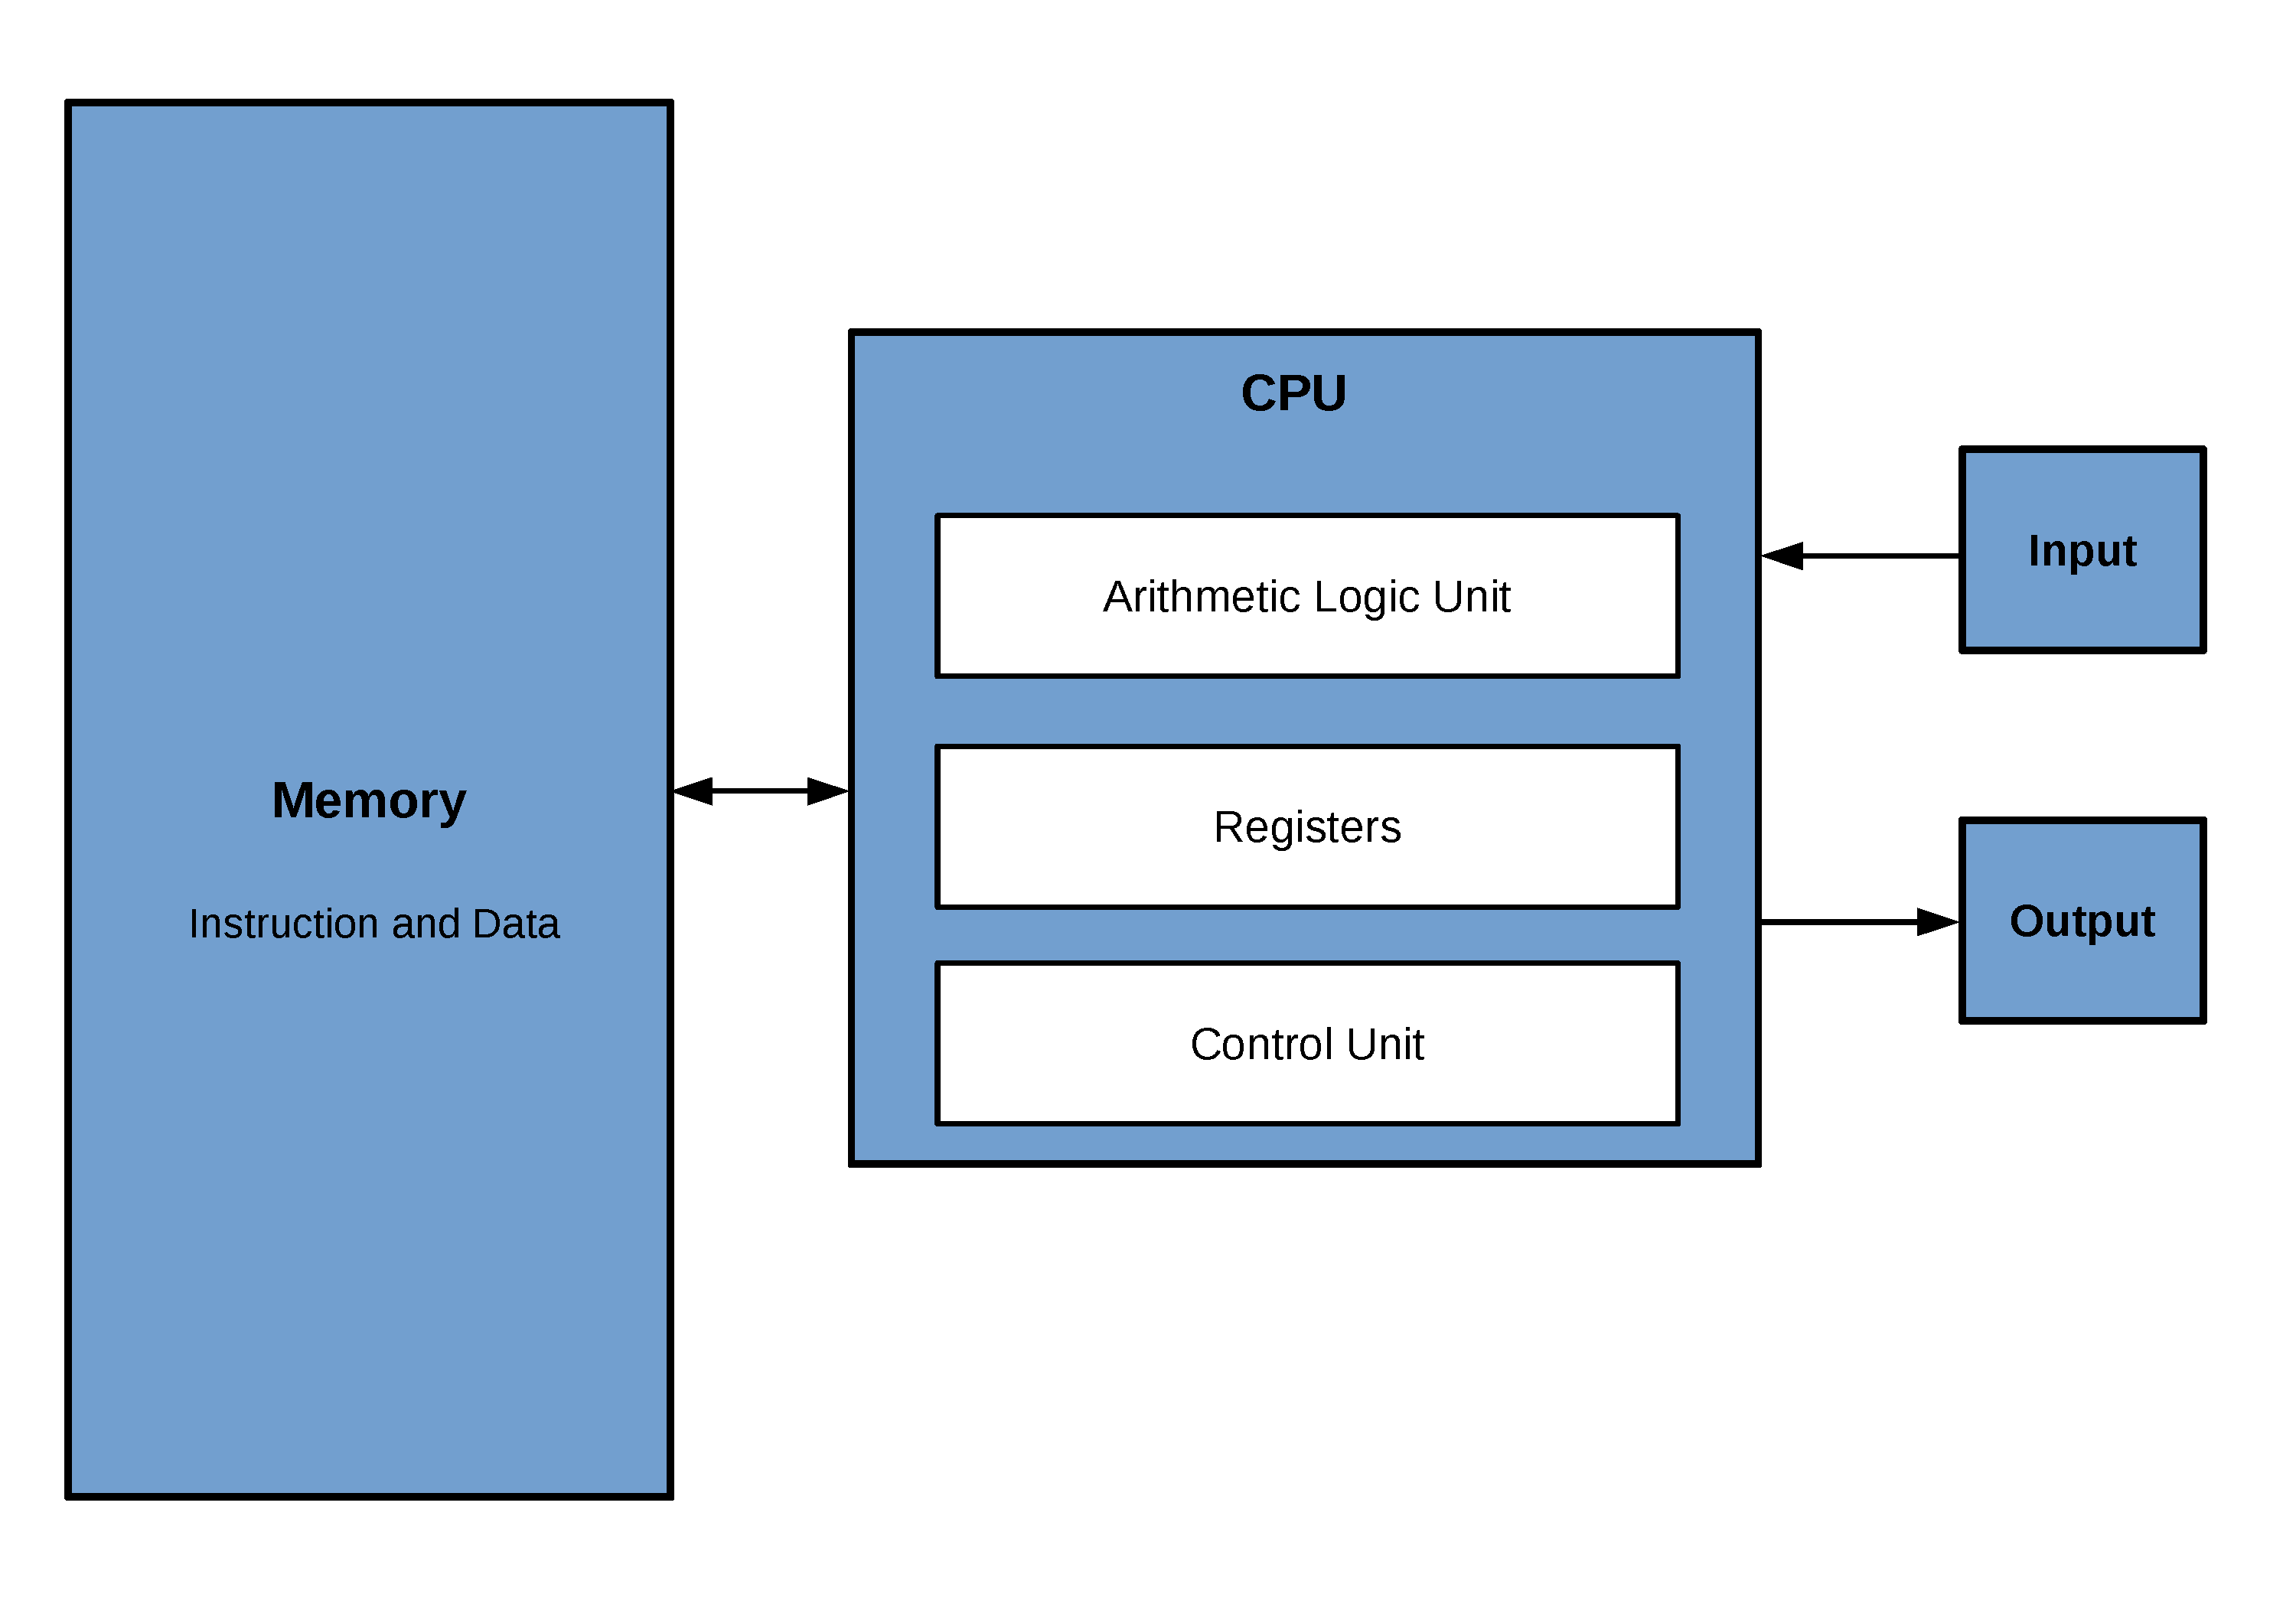
\includegraphics[width=10cm]{von_neumann.pdf}
\end{center}

\end{frame}

\begin{frame}%[fragile]
\frametitle{The Von Neumann Model}

\vspace{-0.2cm}

\begin{center}
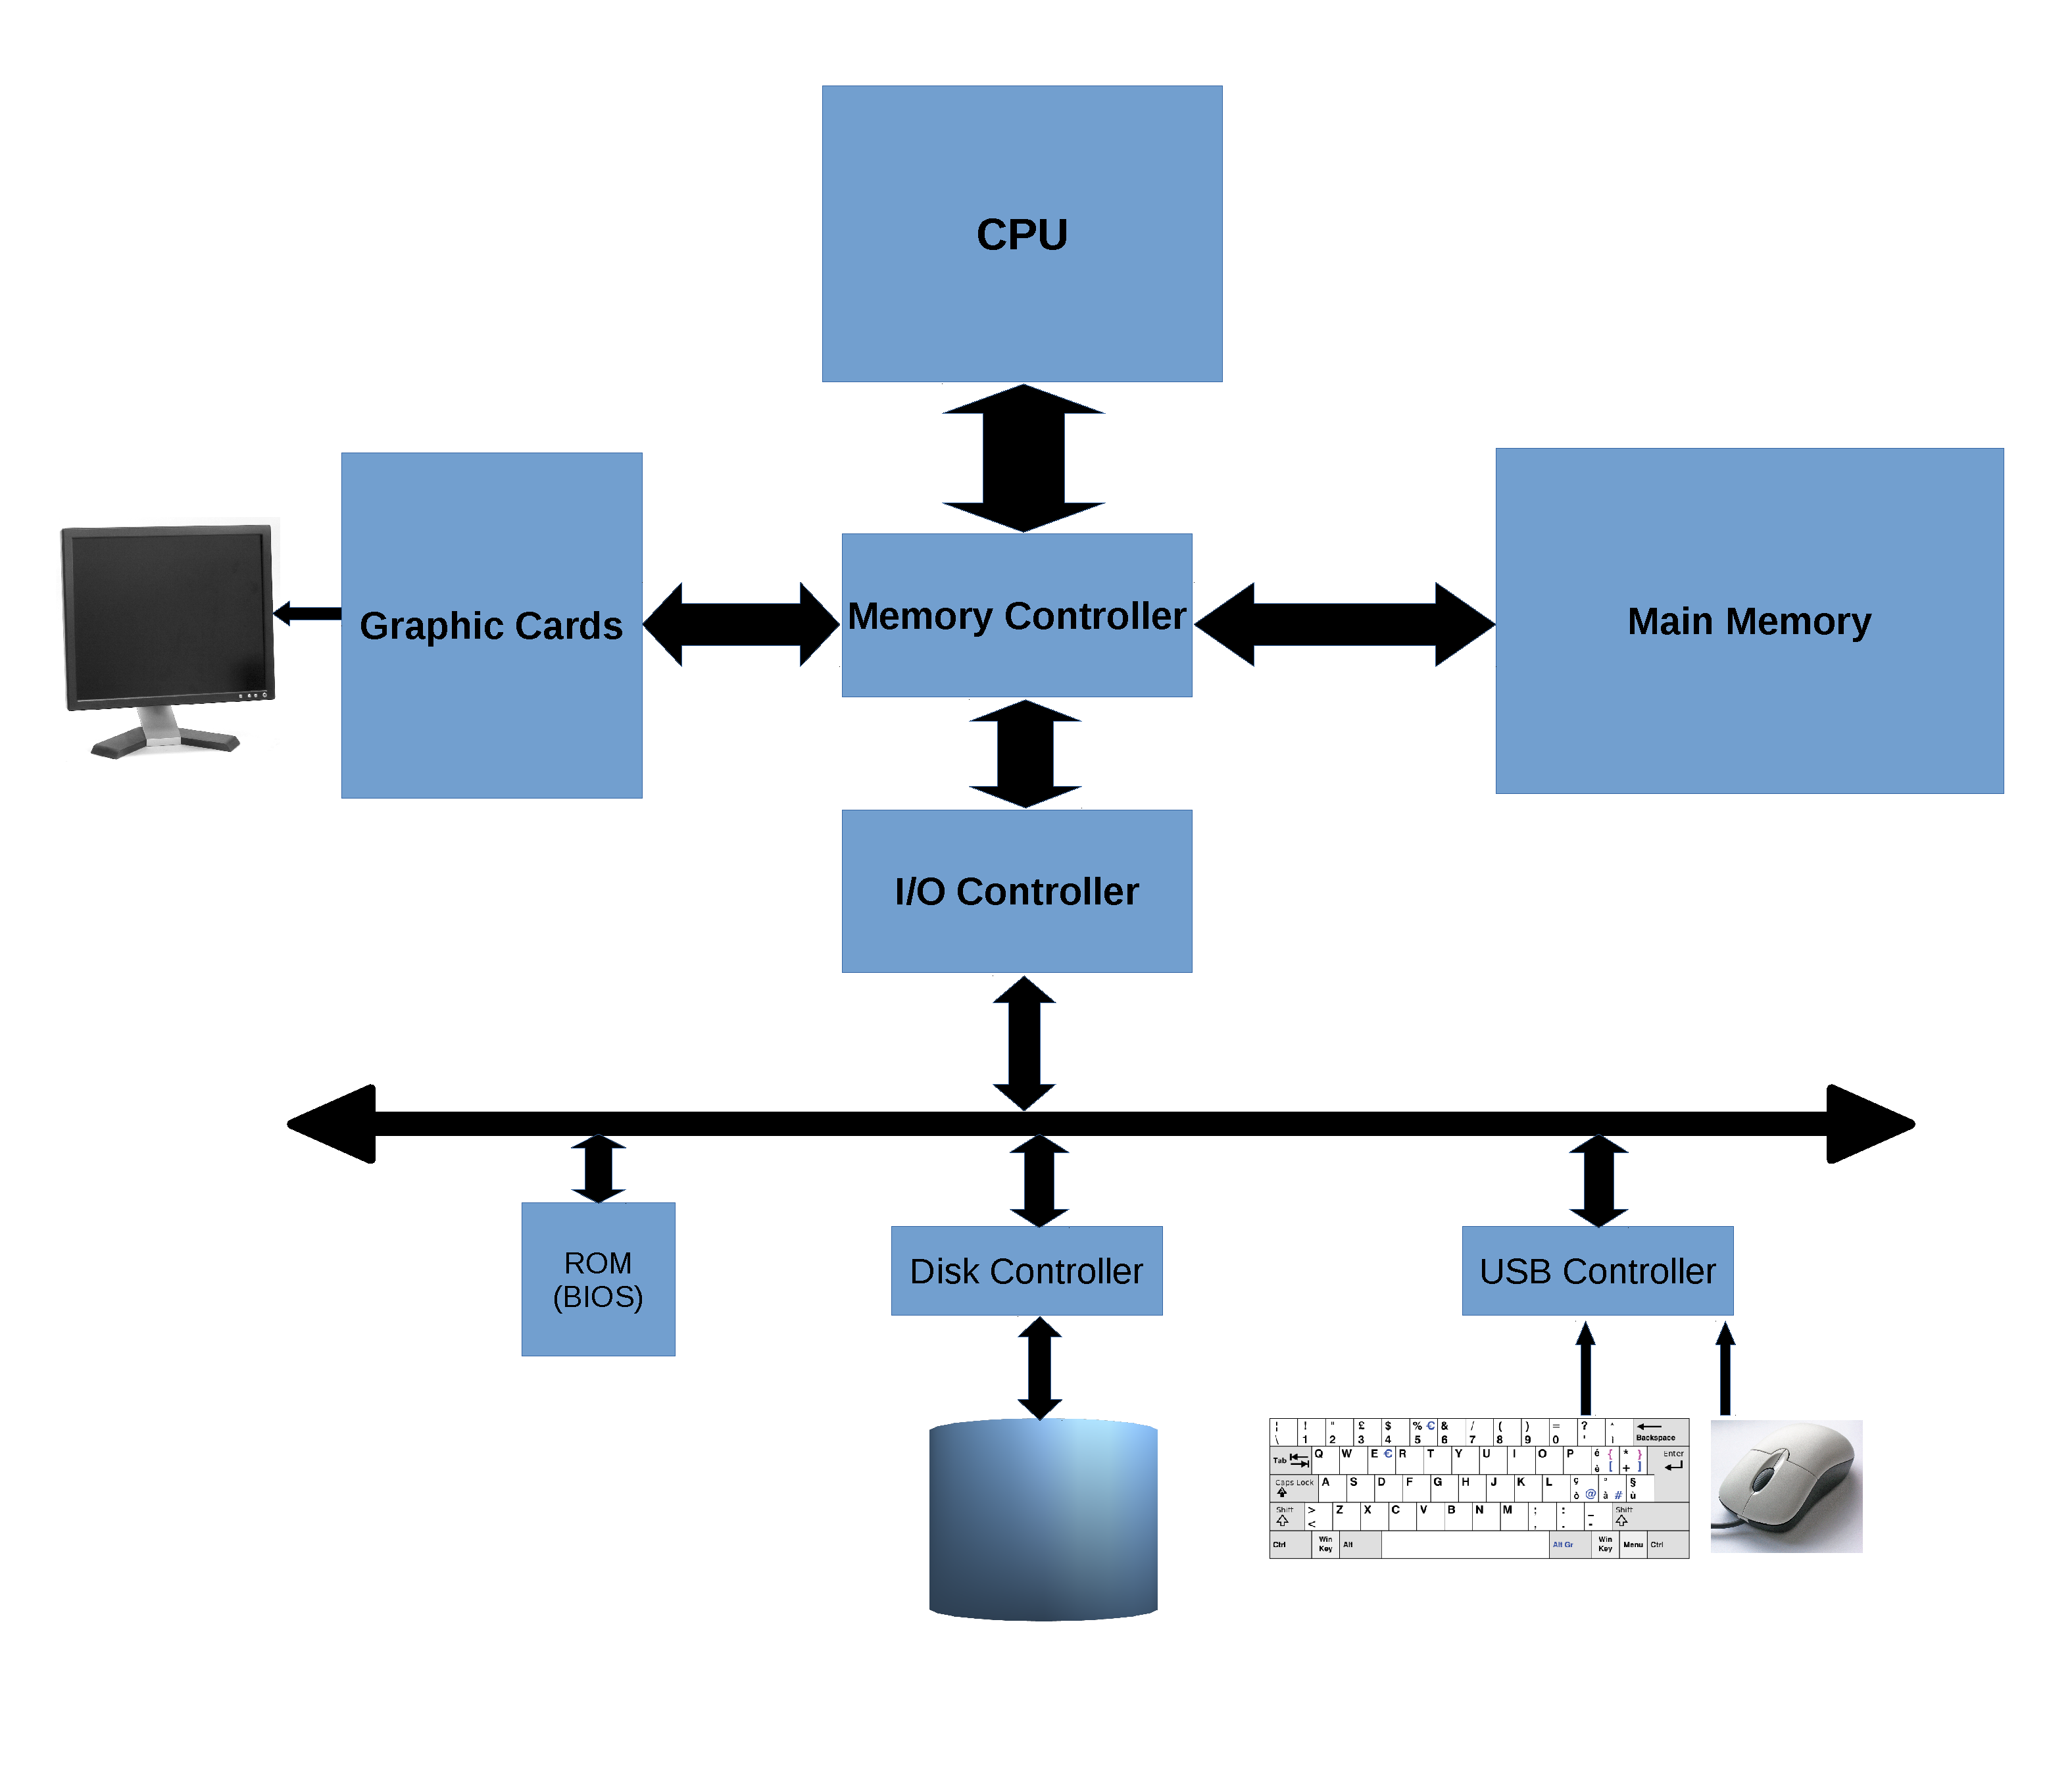
\includegraphics[width=8.5cm]{von_neumann2.pdf}
\end{center}

\end{frame}

\begin{frame}%[fragile]
\frametitle{Real Machine}

\vspace{-0.2cm}

\begin{center}
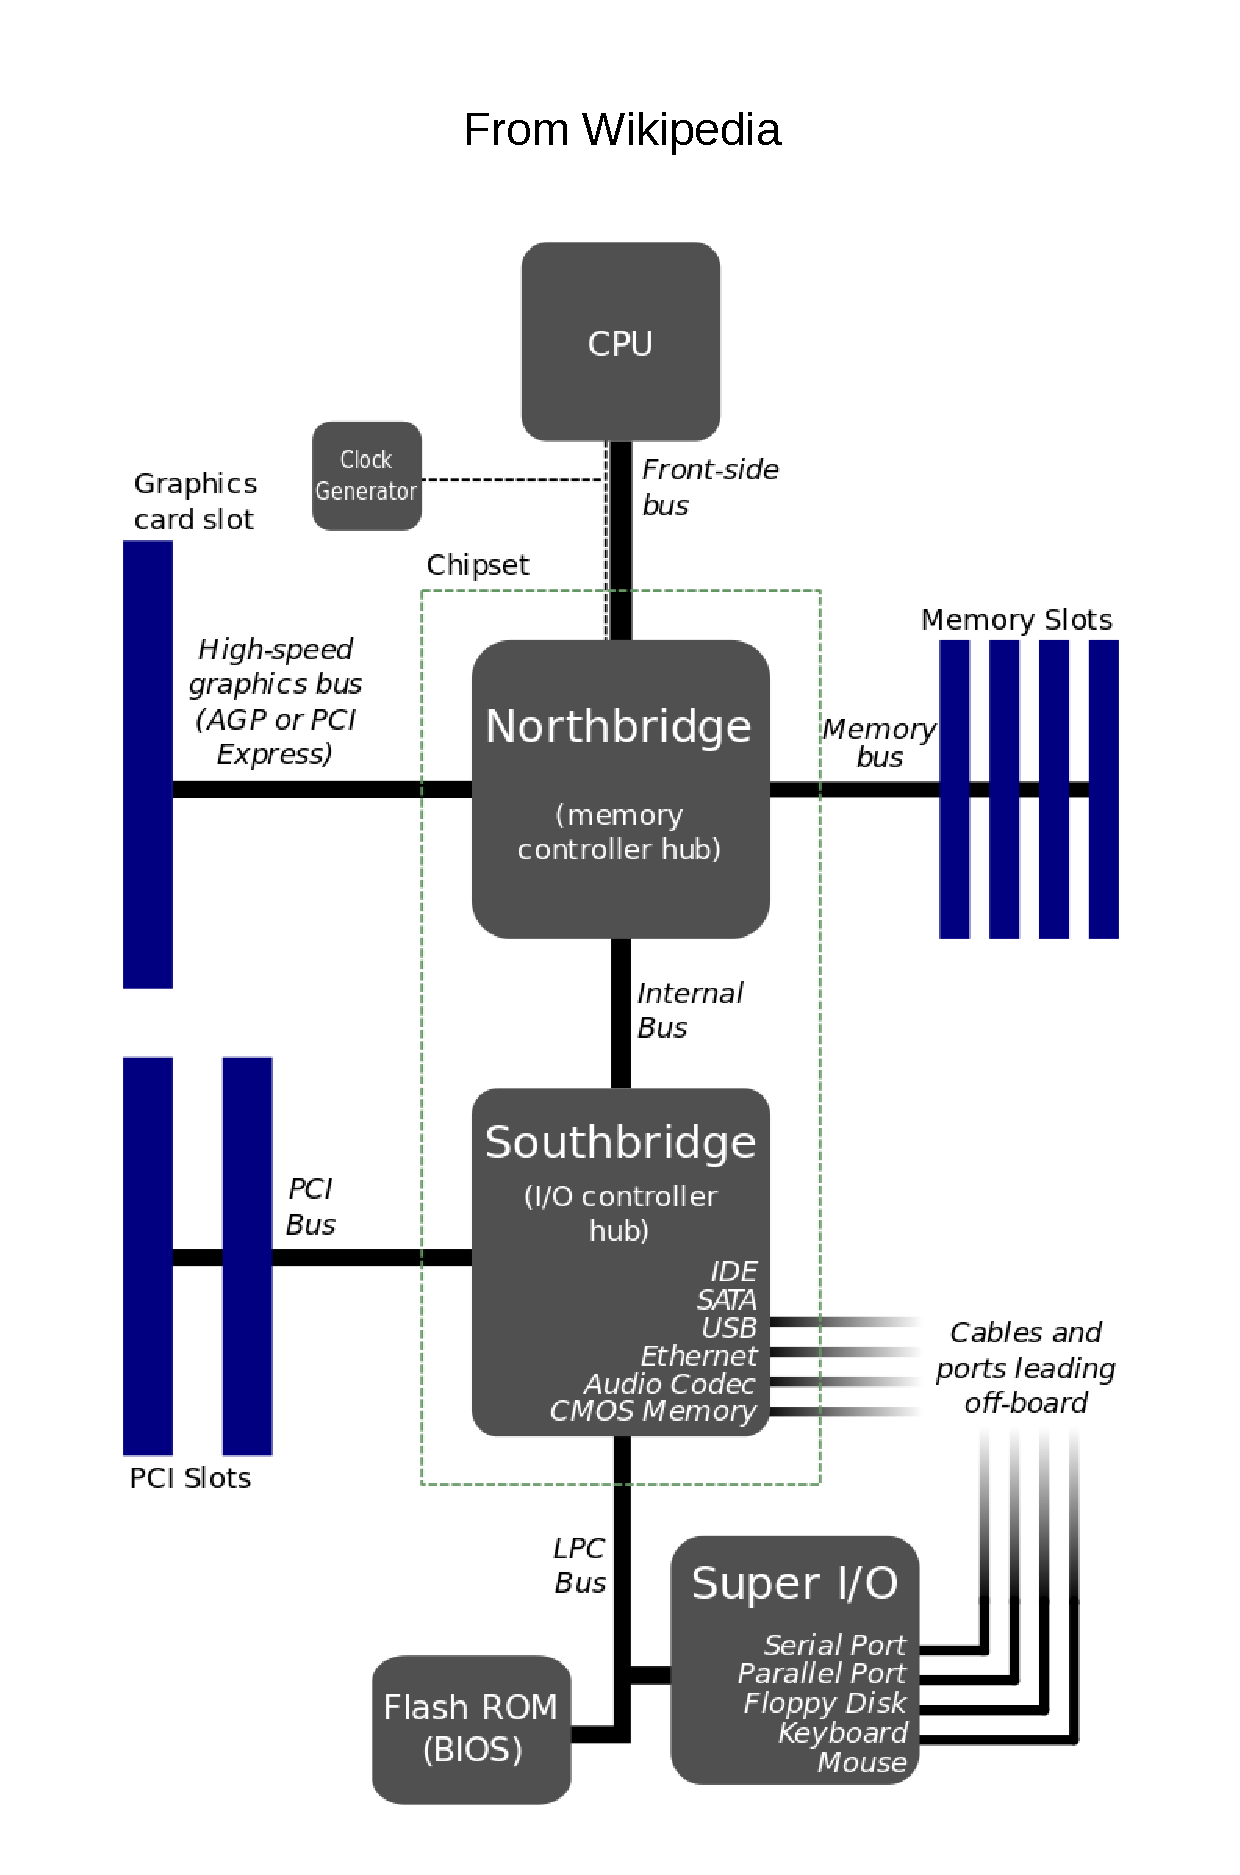
\includegraphics[width=4.7cm]{motherboard.pdf}
\end{center}

\end{frame}

\begin{frame}%[fragile]
\frametitle{Intel Kaby Lake Die}

\vspace{-0.2cm}

\begin{center}
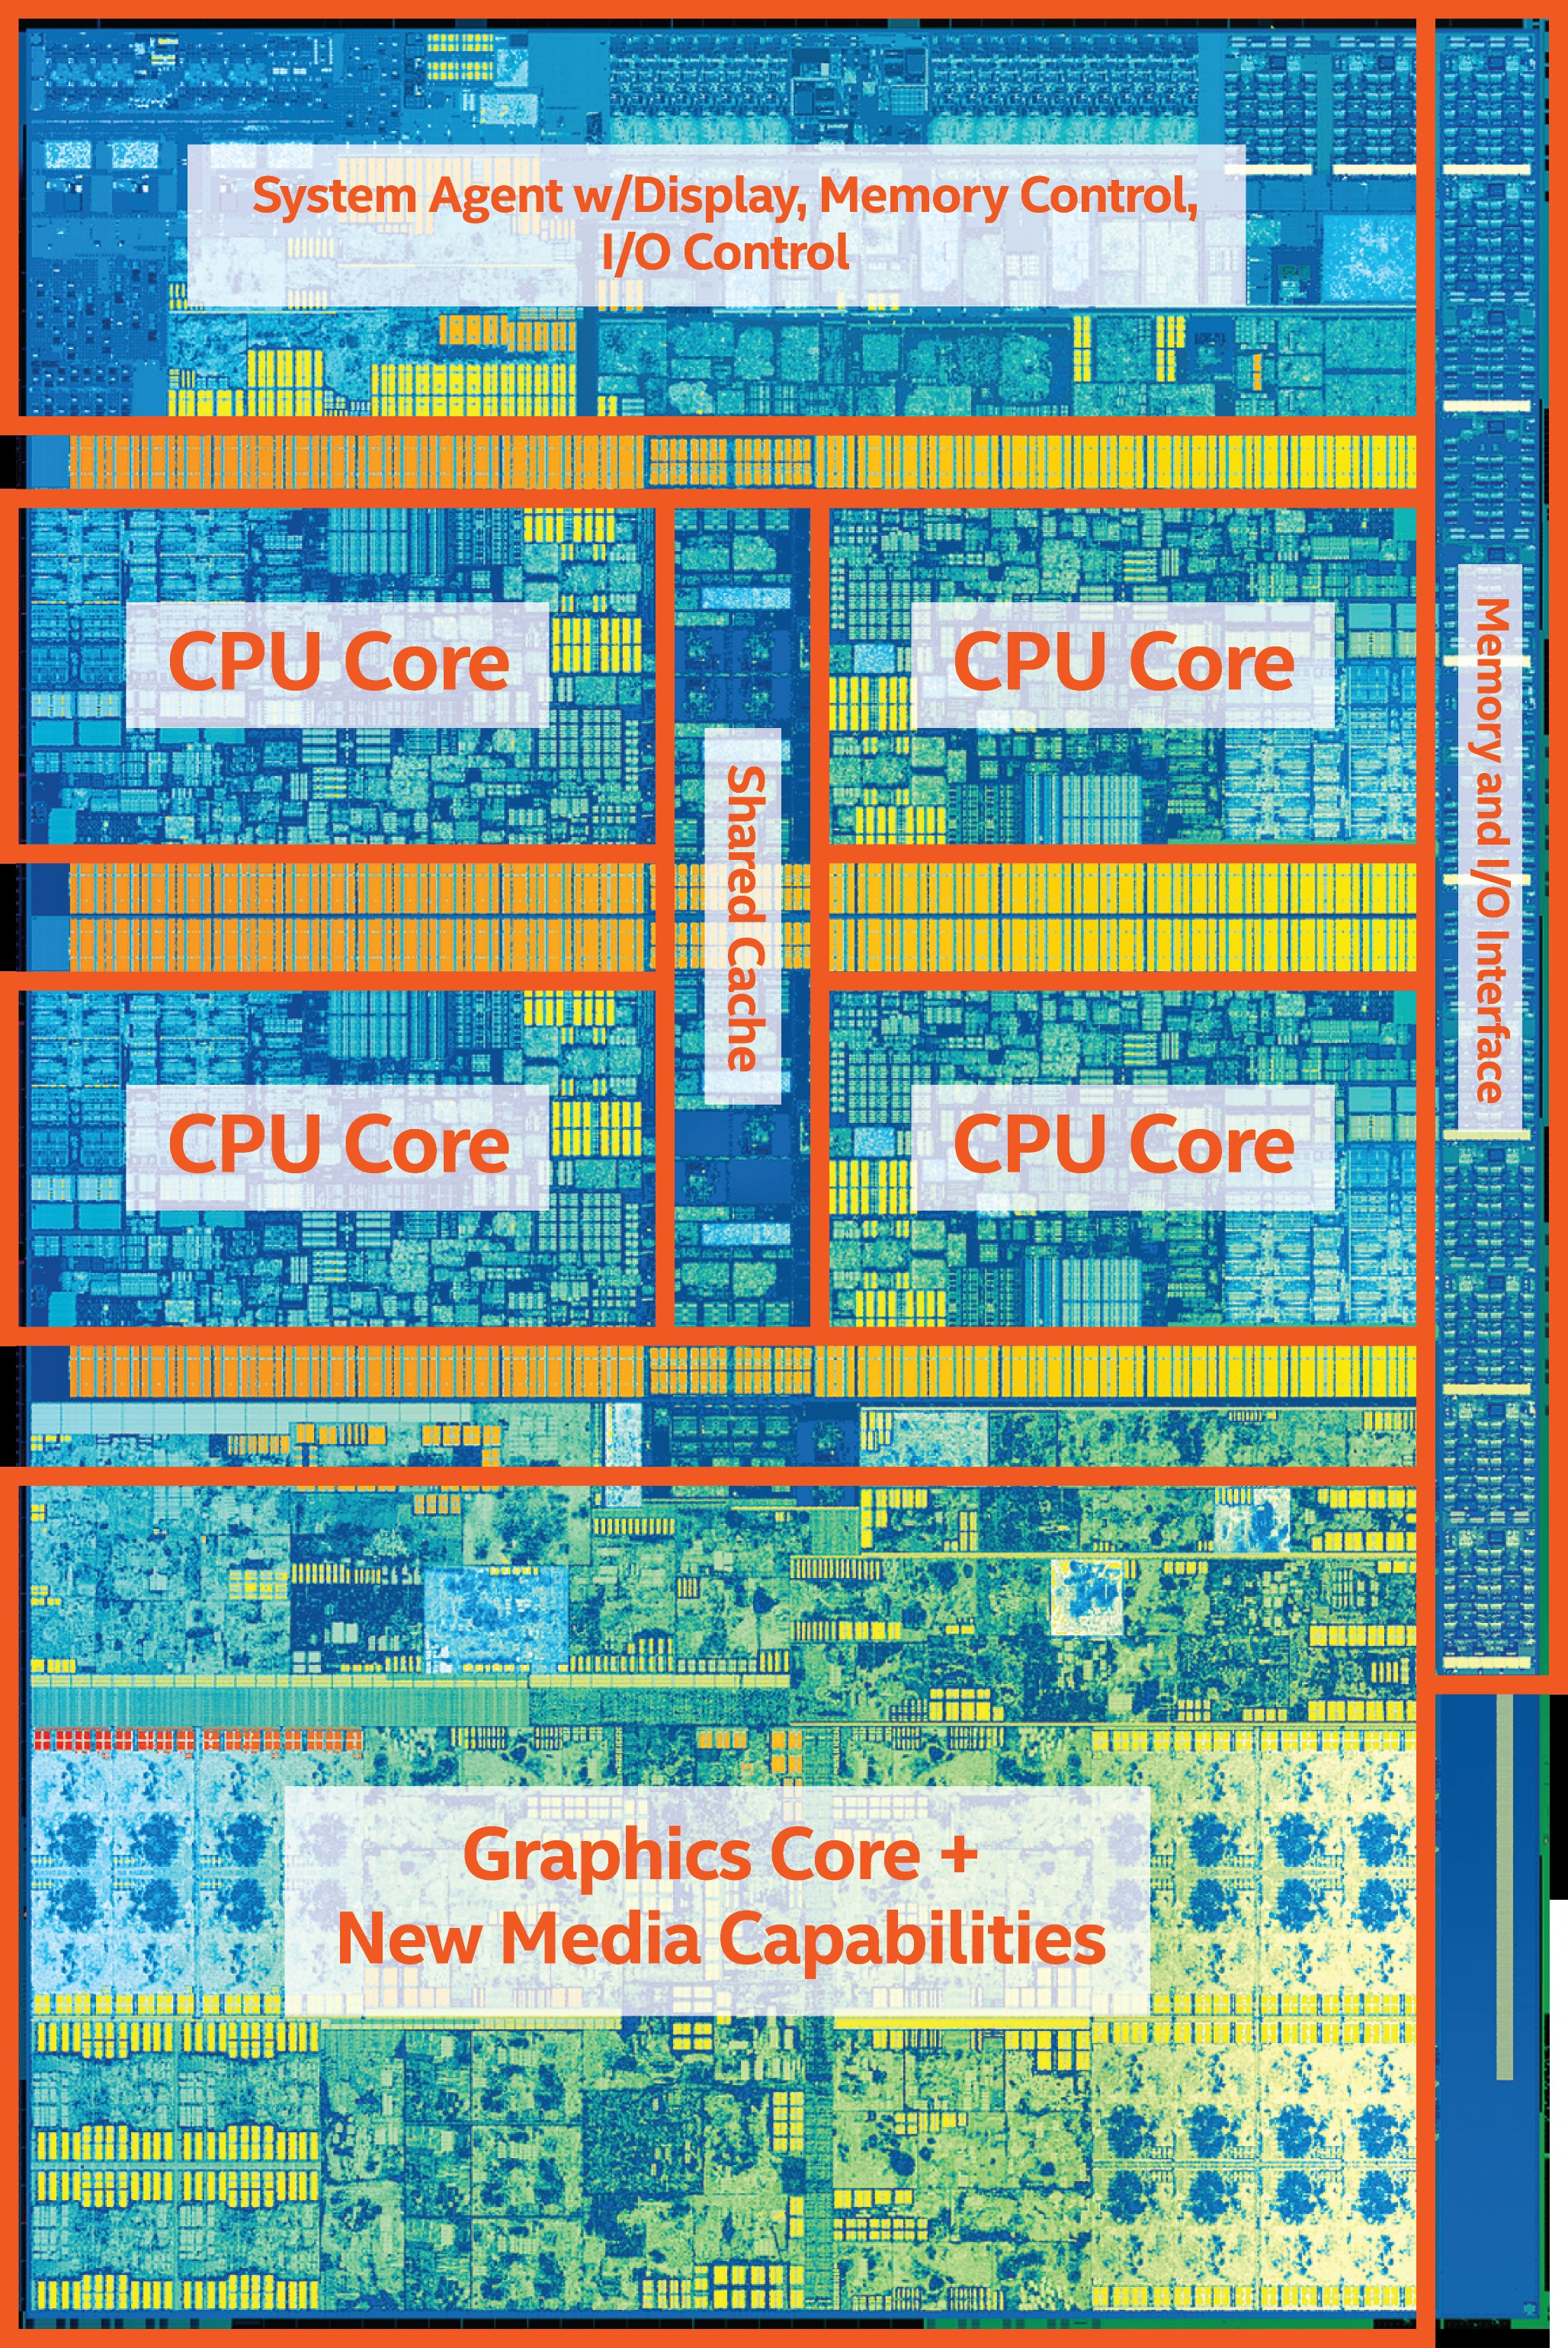
\includegraphics[width=4.7cm]{kabylakedie.jpg}
\end{center}

\end{frame}


\begin{frame}%[fragile]
\frametitle{Intel Kaby Lake Core}

\vspace{-0.2cm}

\begin{center}
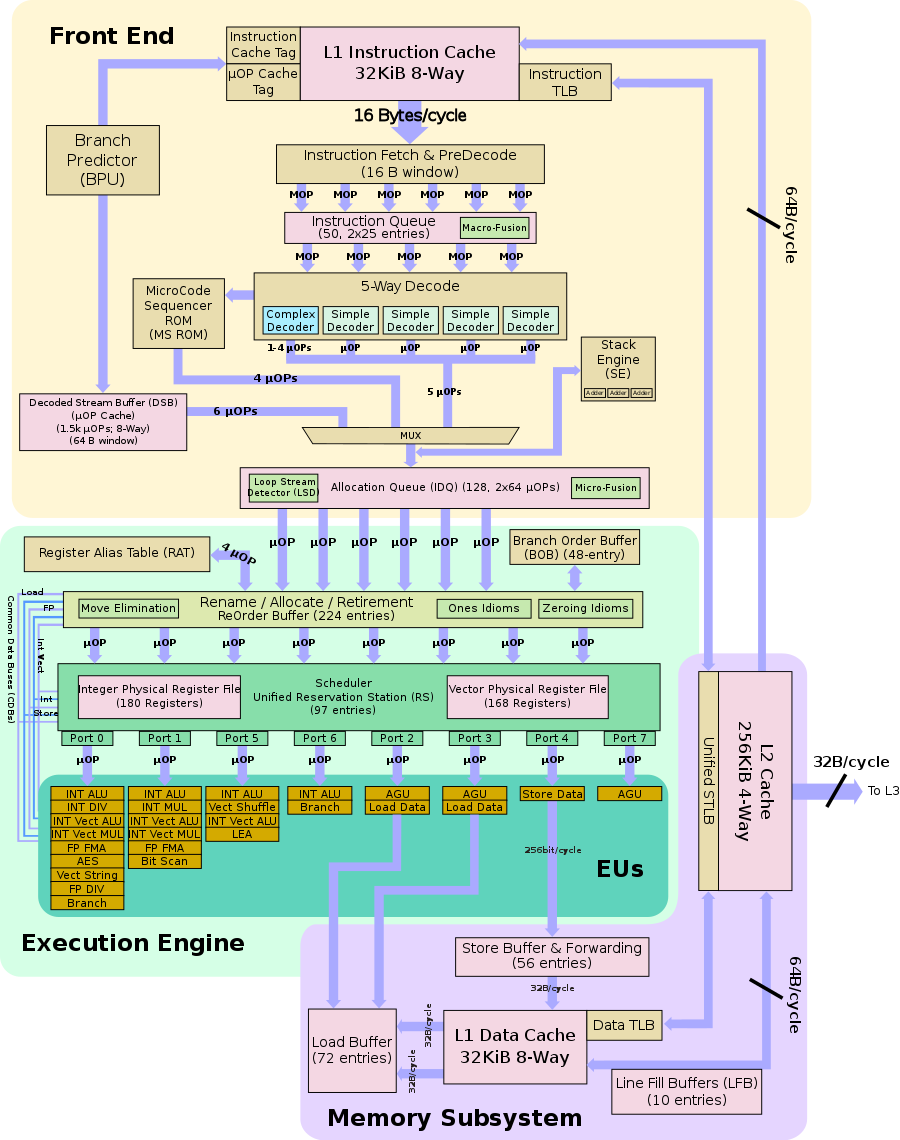
\includegraphics[width=5.5cm]{kabylake.png}
\end{center}

\end{frame}

\begin{frame}%[fragile]
\frametitle{ISA and Microarchitecture}

\begin{itemize}

\item Instruction Set Architecture: The interface between the software and hardware. It provides
  all the information needed for a programmer to write a program in machine language.
  \begin{itemize}
  \item Instruction set.
  \item Registers.
  \item Memory addressing.
  \item Memory ordering.
  \item \ldots
  \end{itemize}

  \vspace{0.5cm}

\item Microarchitecture: Implementation of the architecture.
  \begin{itemize}
  \item Number of caches.
  \item Cache sizes.
  \item Number of cores.
  \item Clock frequency.
  \item \ldots
  \end{itemize}
\end{itemize}

\end{frame}

\begin{frame}%[fragile]
\frametitle{UltimateRISC: Single Instruction Machine}

\begin{itemize}

\item Only one instruction!

\vspace{0.35cm}

\item \texttt{urisc A, B, JUMP}
  \begin{itemize}
  \item \texttt{A}, \texttt{B} and \texttt{JUMP} are memory addresses.
  \item \texttt{*A} $\leftarrow$ \texttt{*A}\ $-$\ \texttt{*B}.
  \item If result is $<0$ the program counter is set to \texttt{JUMP}, otherwise the
    program counter is incremented.
  \end{itemize}

  \vspace{0.35cm}

\item Memory addresses are $10$ bits wide.

  \vspace{0.35cm}

\item Integers are represented in $30$ bits two's complement.
\end{itemize}

\end{frame}

\begin{frame}[fragile]
\frametitle{UltimateRISC: Single Instruction Machine}

We can simulate \texttt{\textcolor{blue}{mov} A, B} which computes \texttt{*A} $\leftarrow$ \texttt{*B} with\\

\begin{Verbatim}[commandchars=\\\{\}]
0: \textcolor{blue}{urisc} A, A, 1
1: \textcolor{blue}{urisc} C, C, 2
2: \textcolor{blue}{urisc} C, B, 3
3: \textcolor{blue}{urisc} A, C, 4

with C a memory address > 3
     C: don't care
\end{Verbatim}

\end{frame}

\begin{frame}%[fragile]
\frametitle{\exo}

Simulate the instruction\\
\vspace{0.3cm}
\hspace{1cm} \texttt{\textcolor{blue}{add} A, B}\\
\vspace{0.3cm}
which computes\\
\vspace{0.3cm}
\hspace{1cm} \texttt{*A} $\leftarrow$ \texttt{*A}\ $+$\ \texttt{*B}.

\end{frame}

\ifanswers

\begin{frame}[fragile]
\frametitle{Solution}

\begin{Verbatim}[commandchars=\\\{\}]
0: \textcolor{blue}{urisc} C, C, 1
1: \textcolor{blue}{urisc} C, B, 2
2: \textcolor{blue}{urisc} A, C, 3

with C a memory address > 2
     C: don't care
\end{Verbatim}

\end{frame}

\fi

\begin{frame}%[fragile]
\frametitle{UltimateRISC}

\vspace{-0.2cm}

\begin{center}
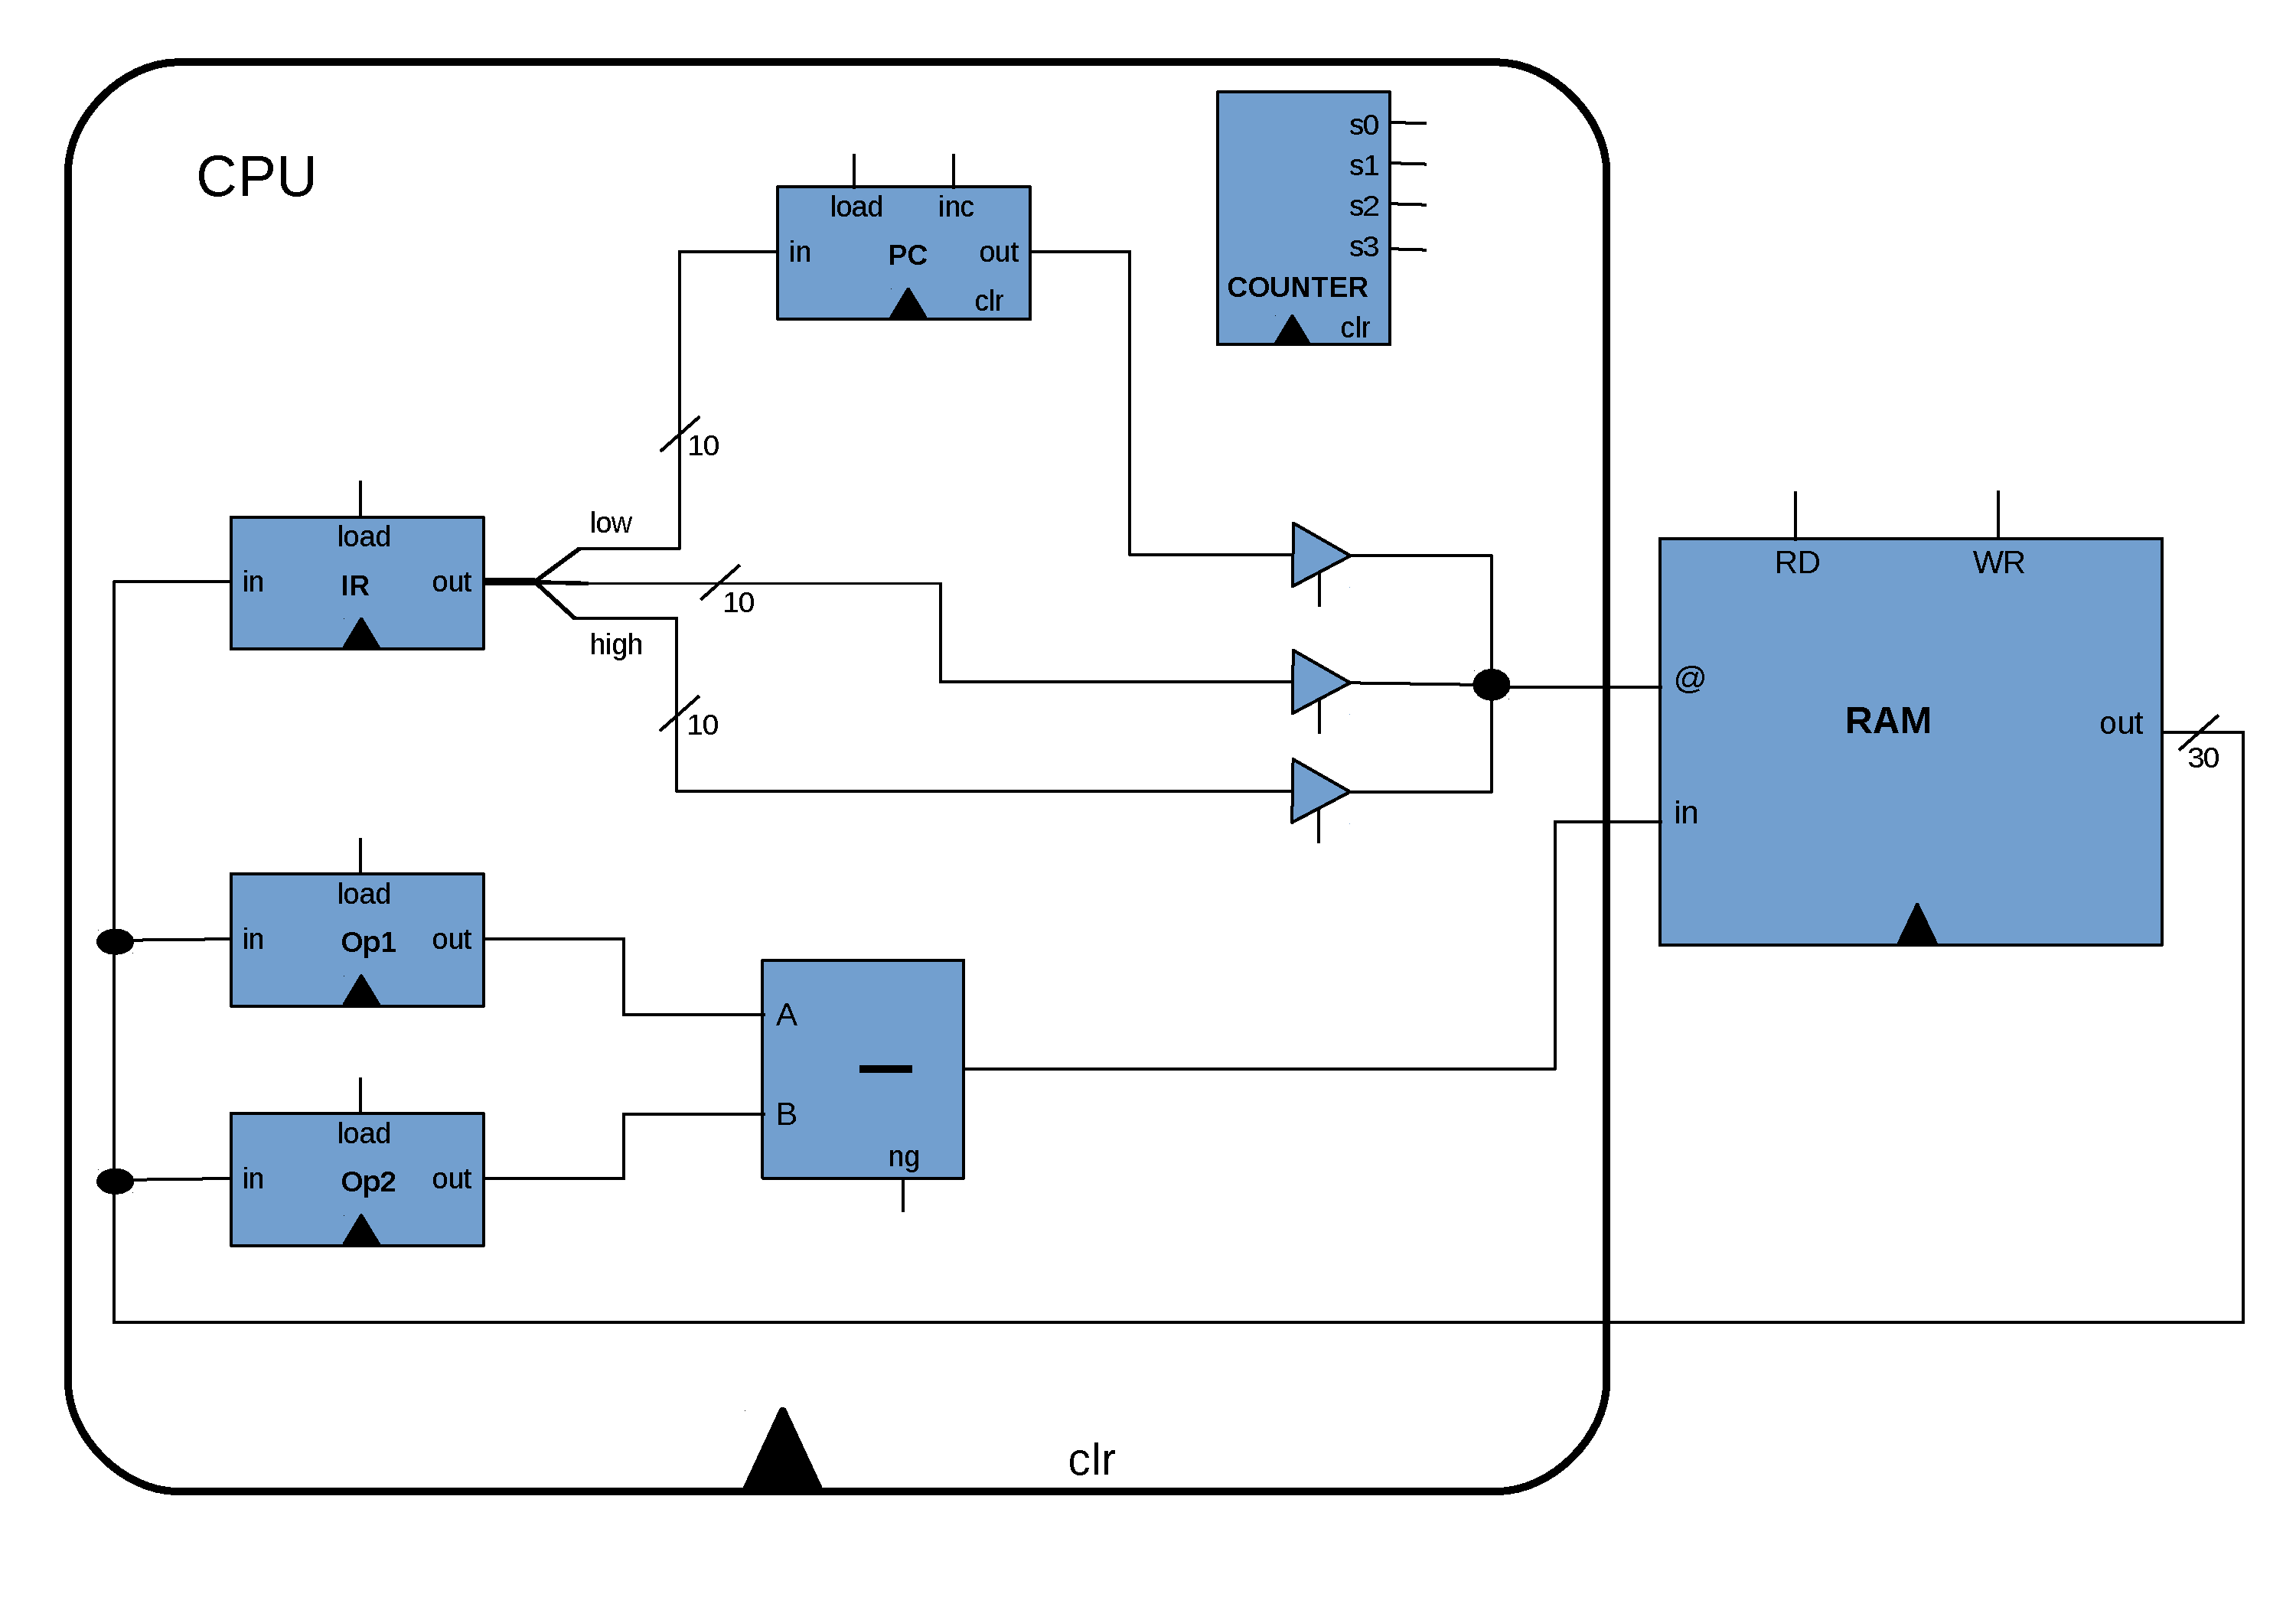
\includegraphics[width=10.8cm]{urisc.pdf}
\end{center}

\end{frame}

\begin{frame}%[fragile]
\frametitle{UltimateRISC}

\vspace{-0.2cm}

\begin{center}
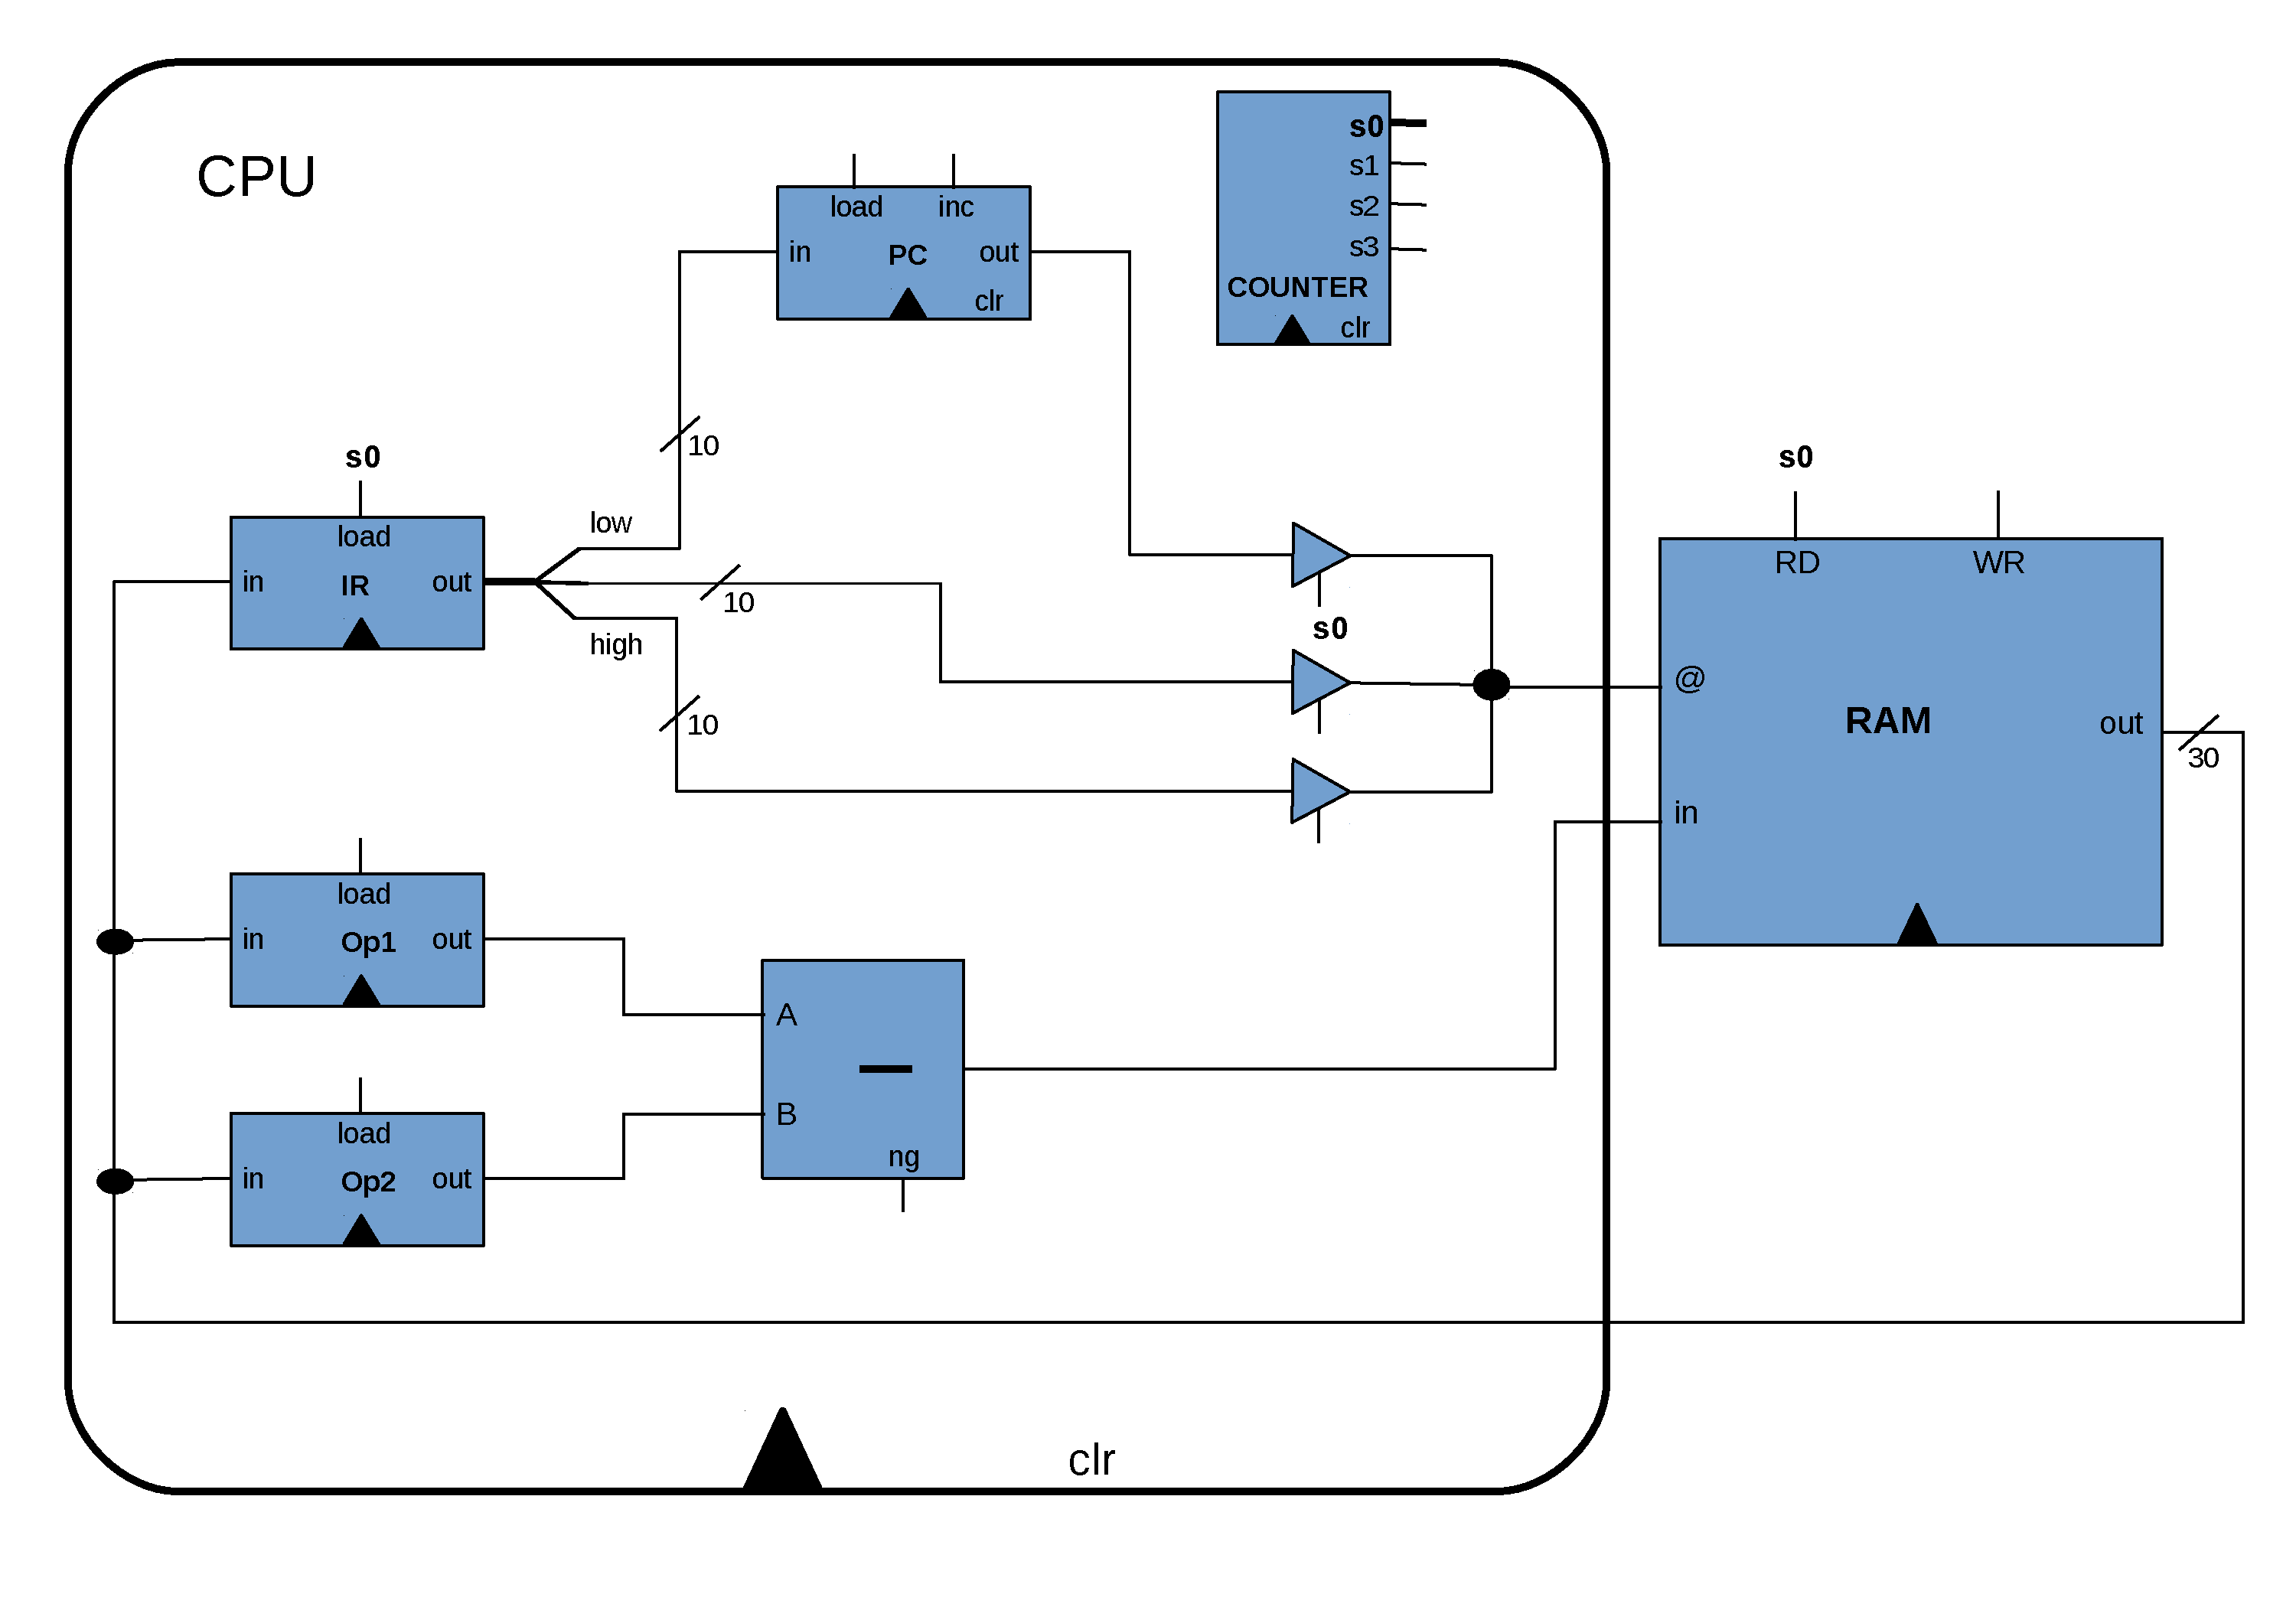
\includegraphics[width=10.8cm]{urisc1.pdf}
\end{center}

\end{frame}

\begin{frame}%[fragile]
\frametitle{UltimateRISC}

\vspace{-0.2cm}

\begin{center}
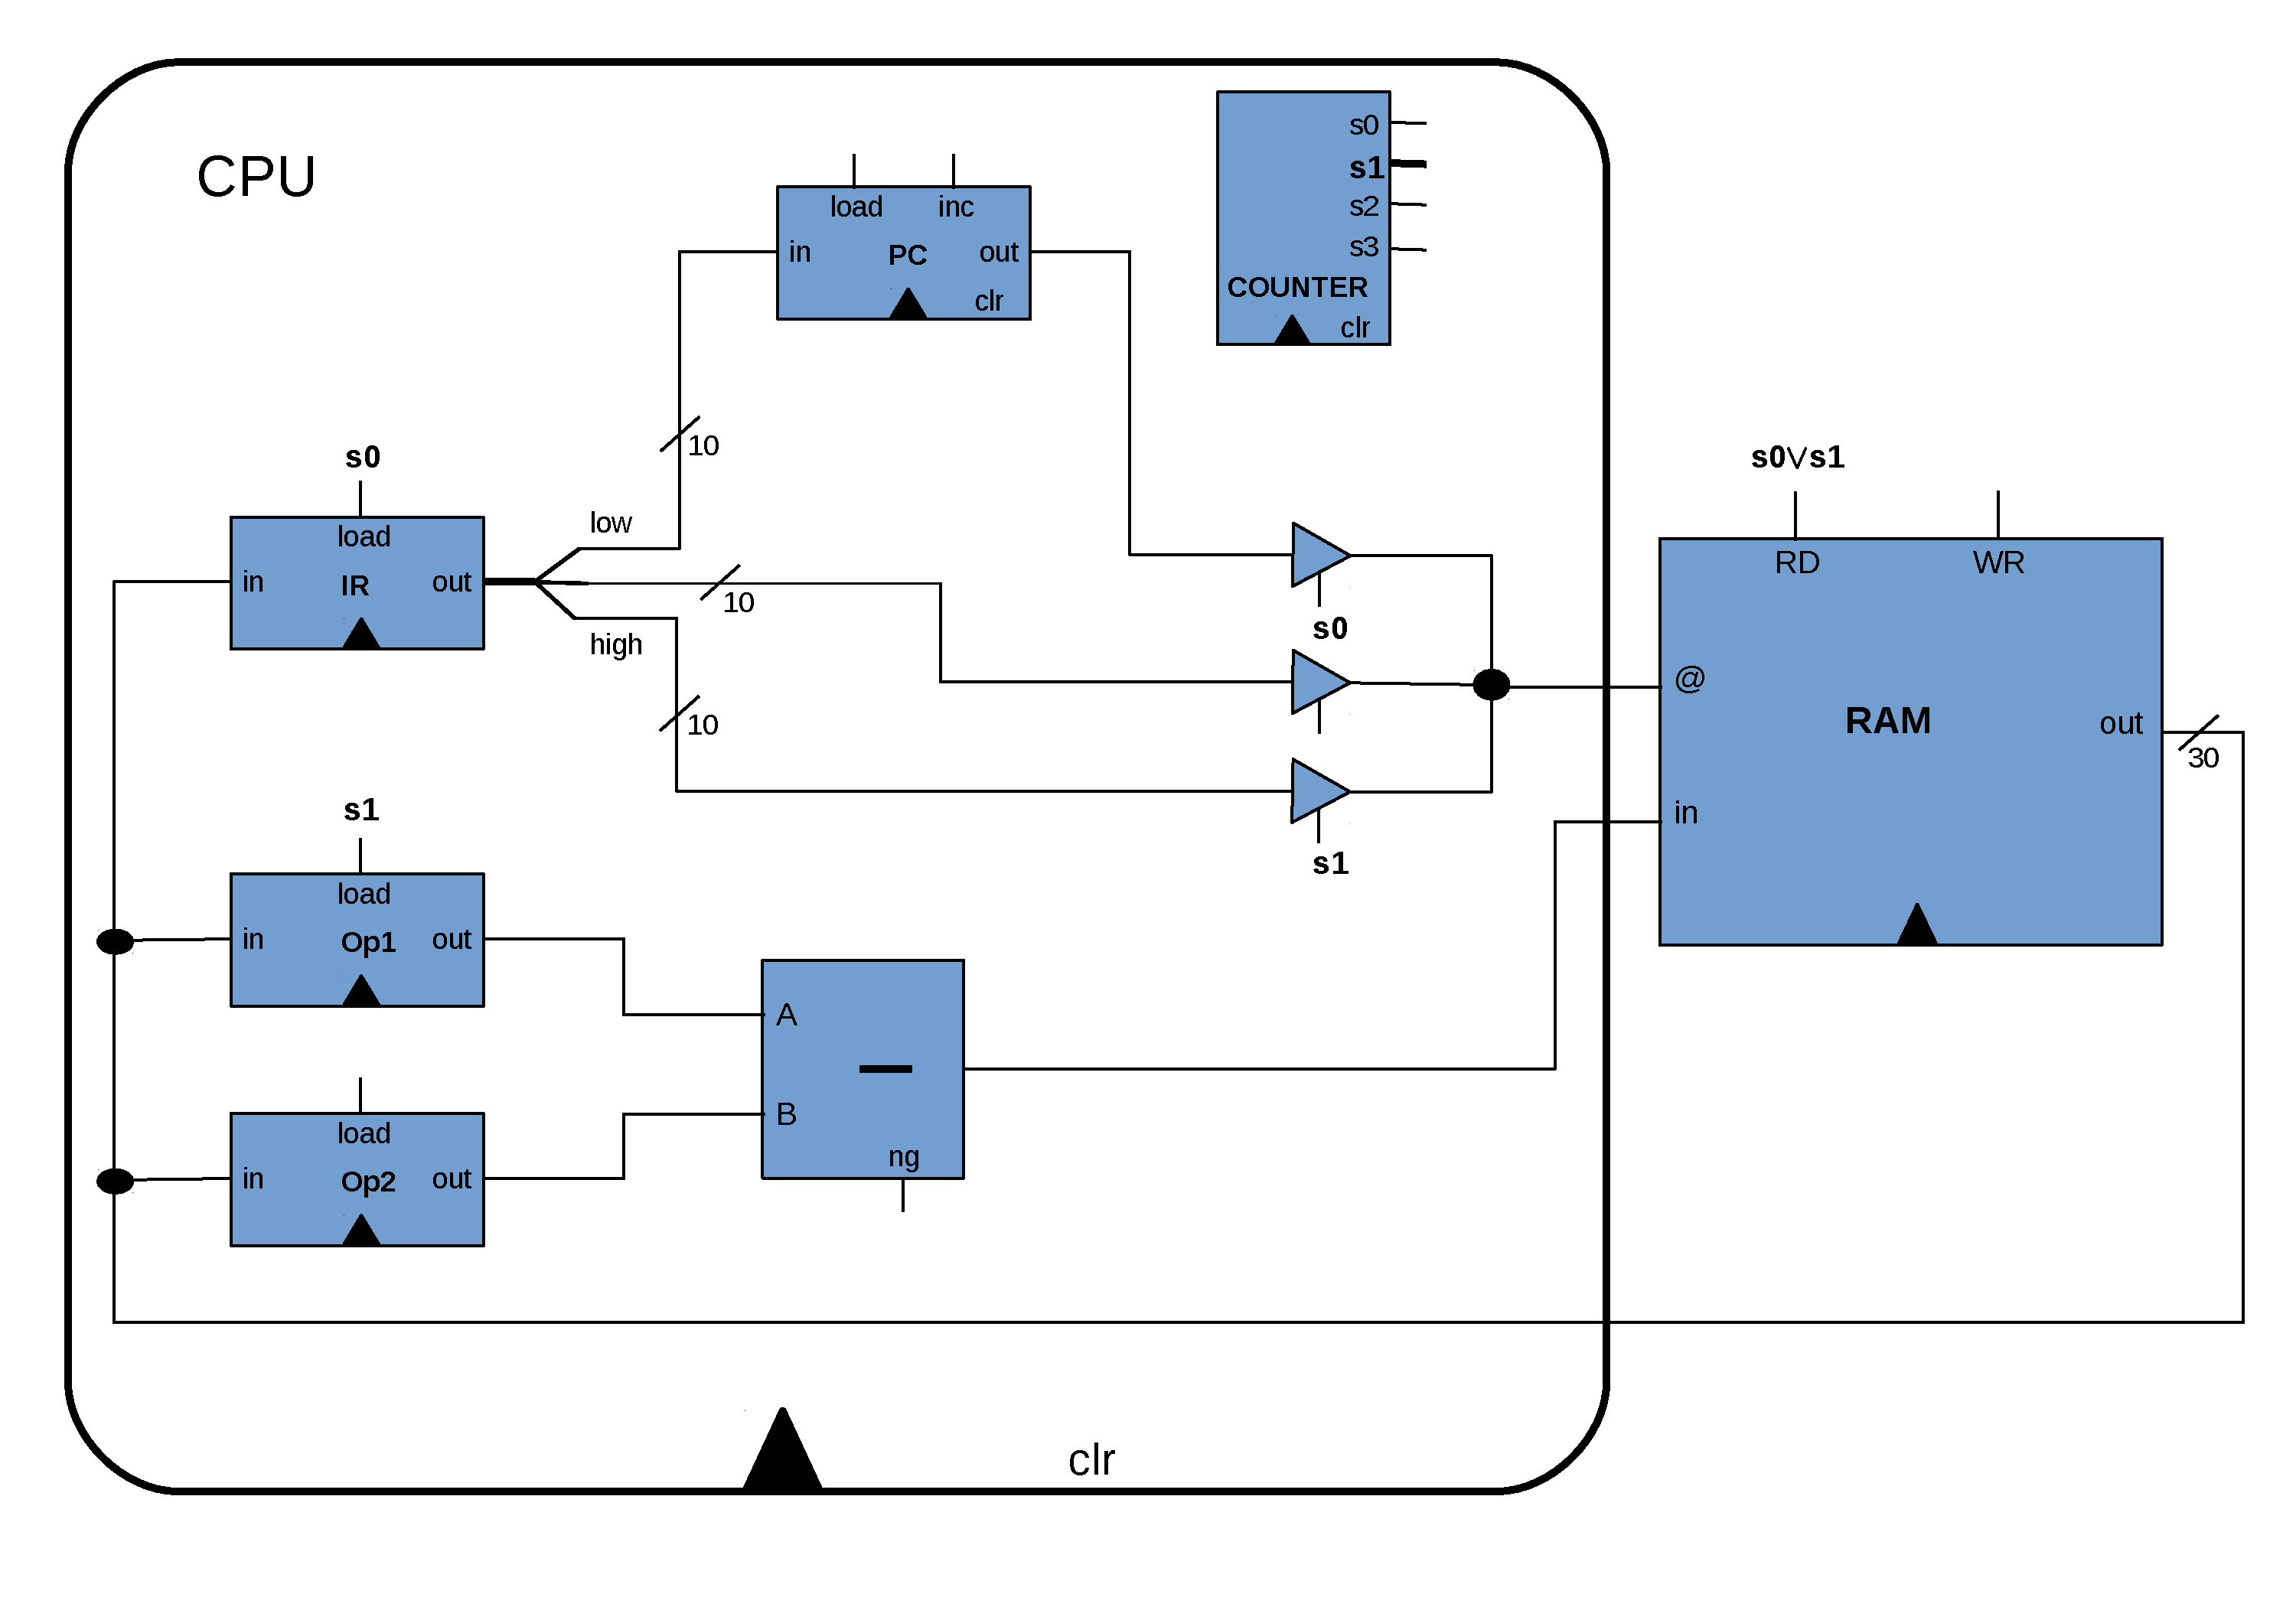
\includegraphics[width=10.8cm]{urisc2.pdf}
\end{center}

\end{frame}

\begin{frame}%[fragile]
\frametitle{UltimateRISC}

\vspace{-0.2cm}

\begin{center}
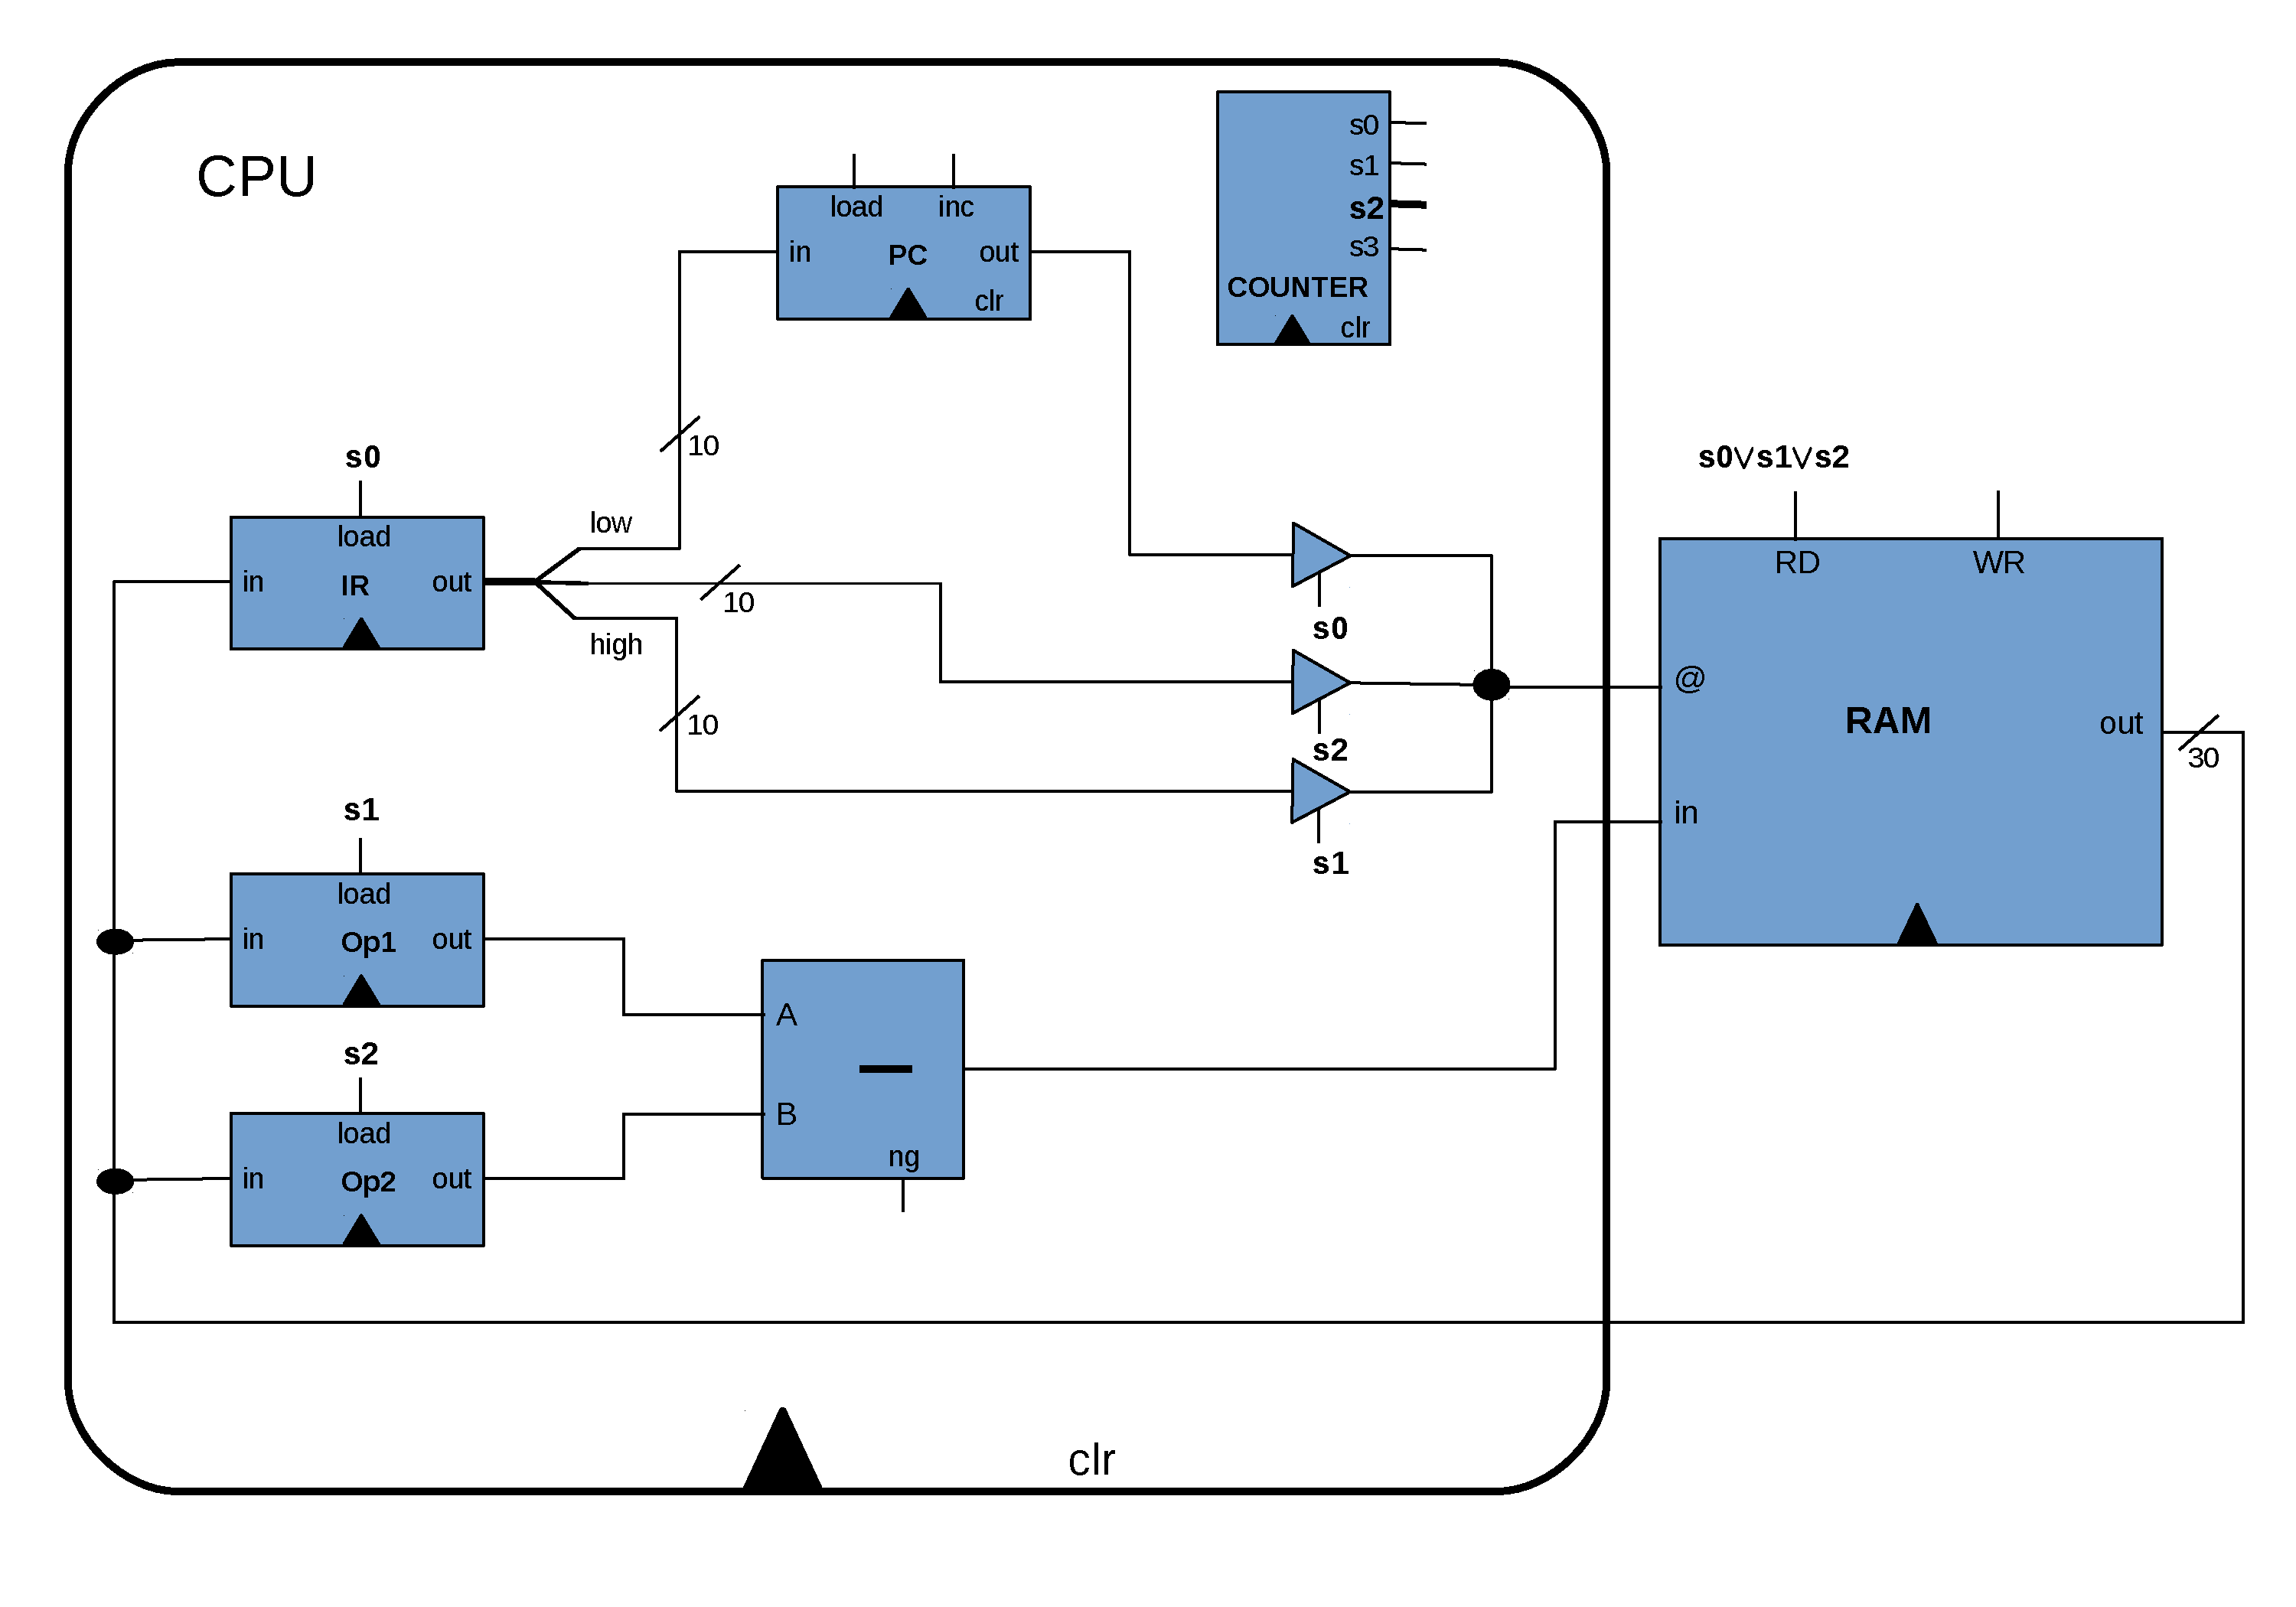
\includegraphics[width=10.8cm]{urisc3.pdf}
\end{center}

\end{frame}

\begin{frame}%[fragile]
\frametitle{UltimateRISC}

\vspace{-0.2cm}

\begin{center}
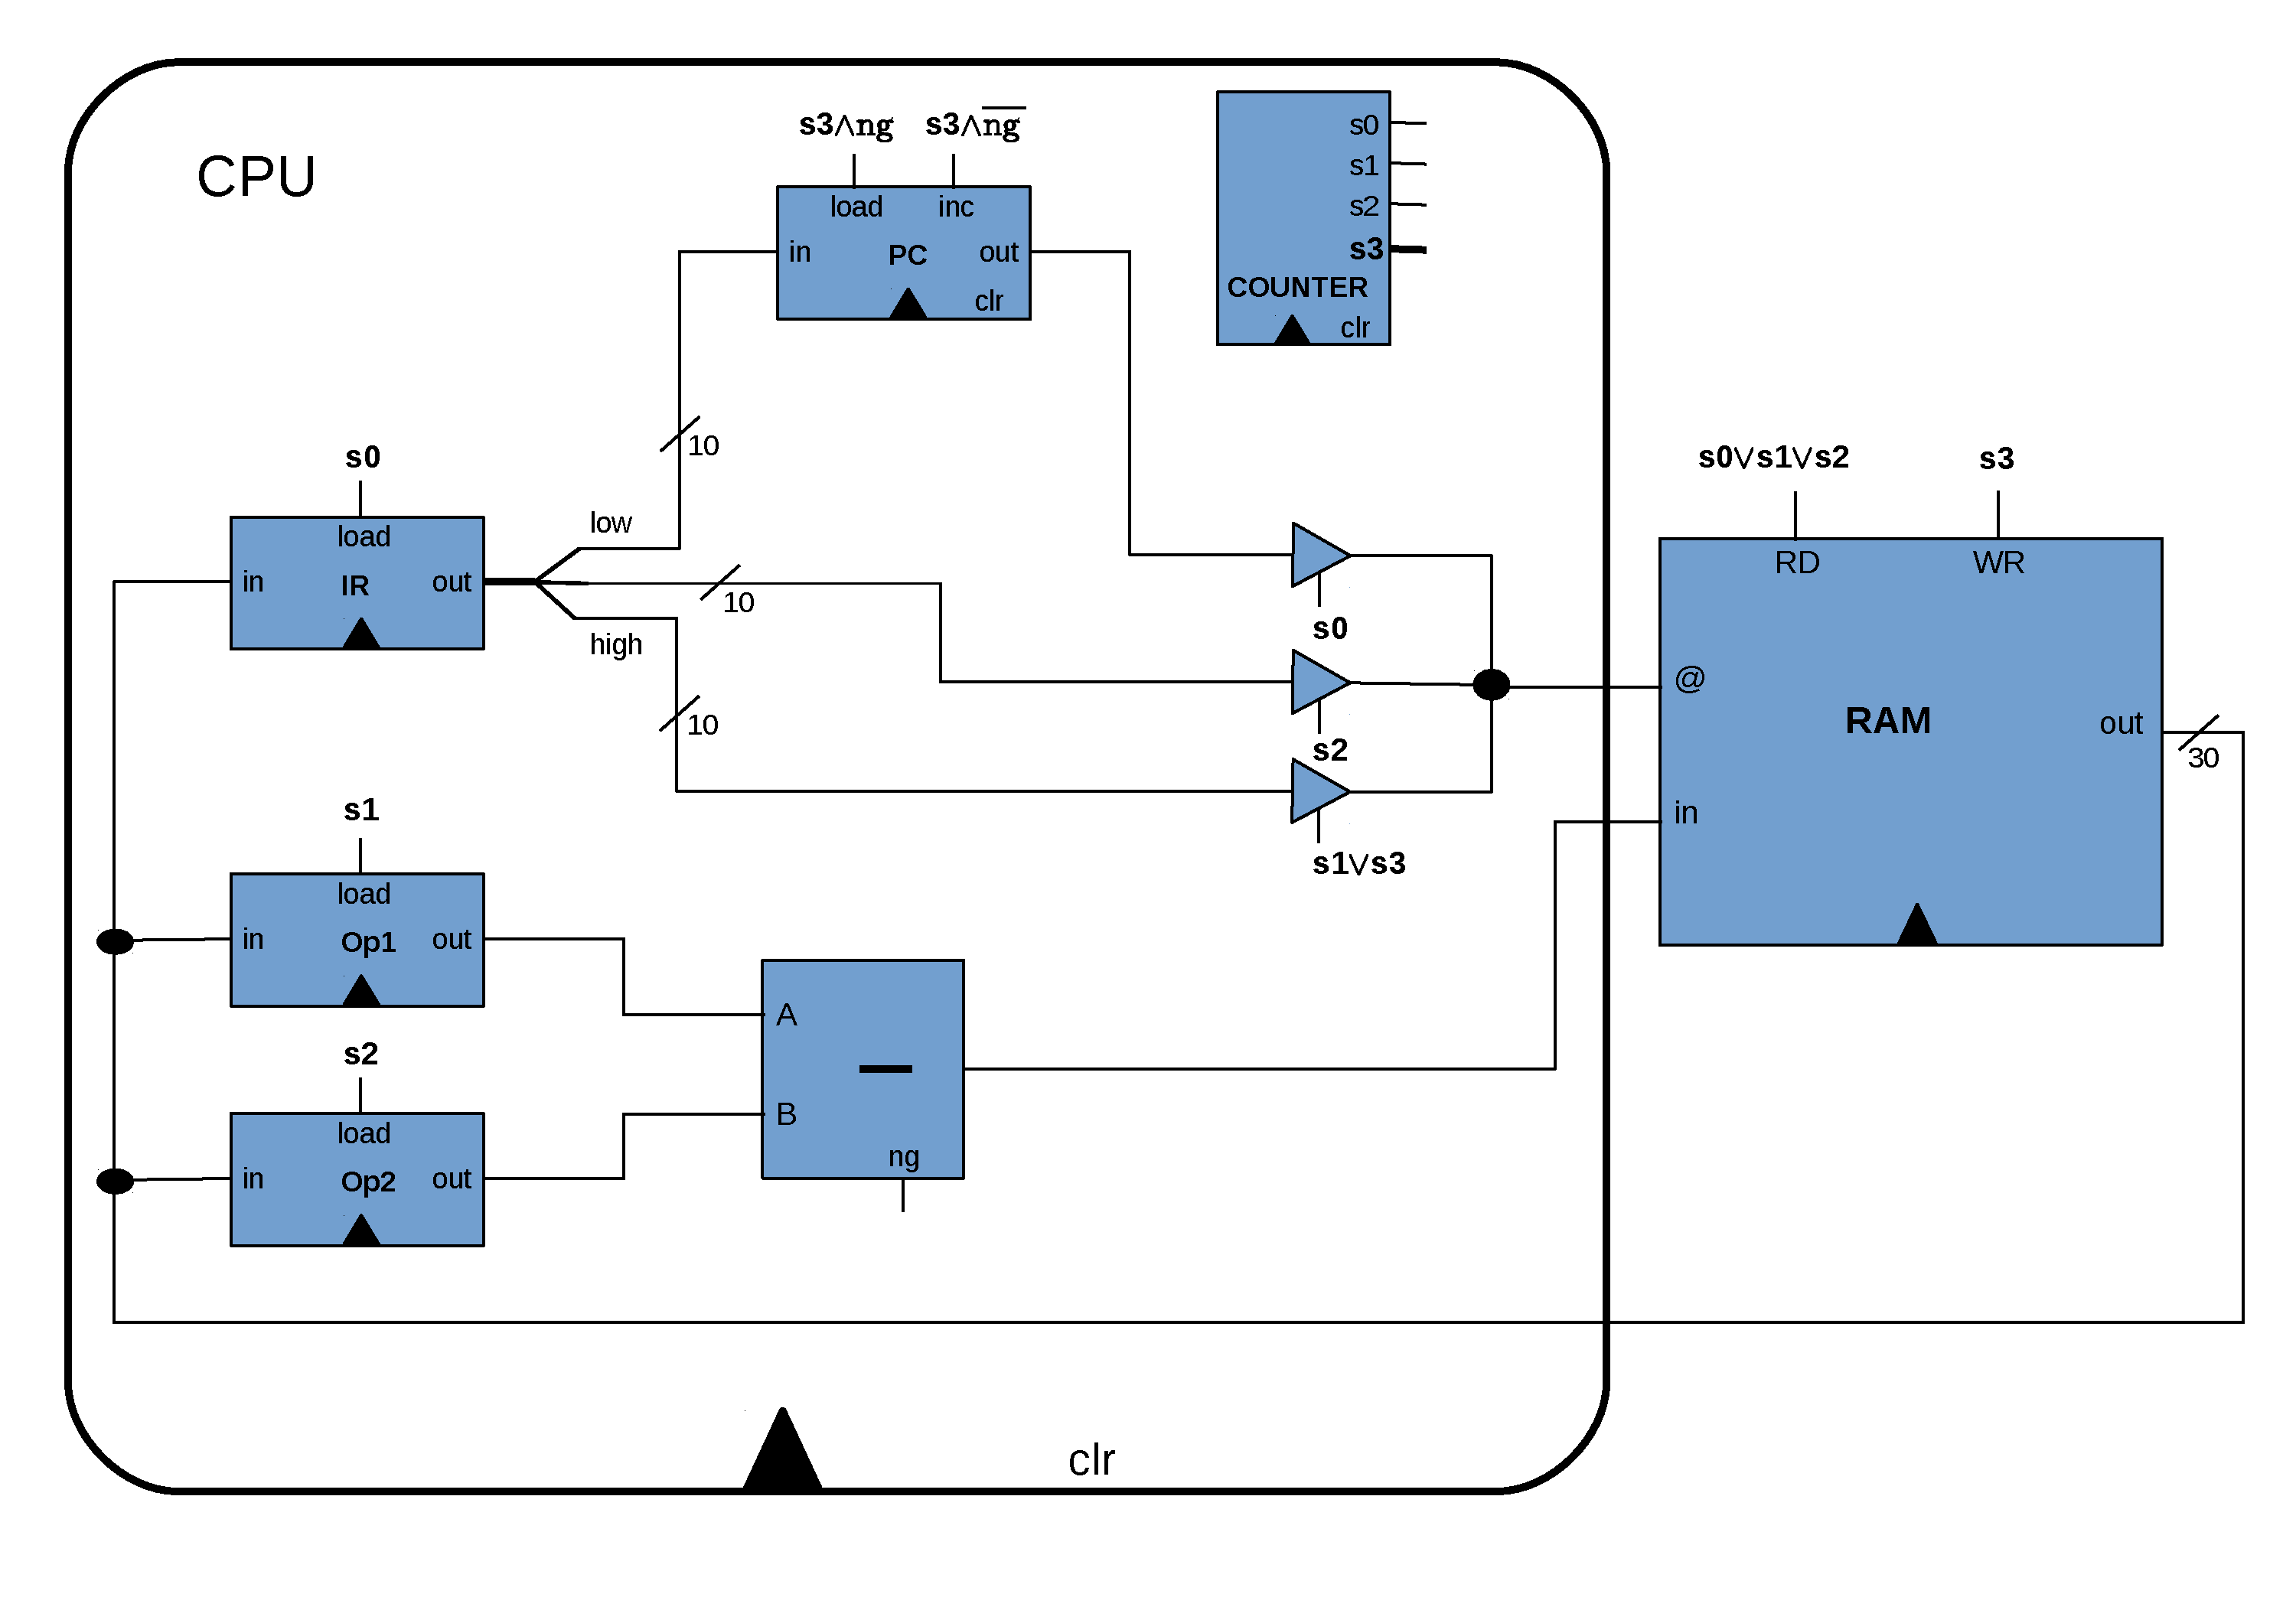
\includegraphics[width=10.8cm]{urisc4.pdf}
\end{center}

\end{frame}

\begin{frame}%[fragile]
\frametitle{MIPS32 with Logisim}

\vspace{-0.2cm}

\begin{center}
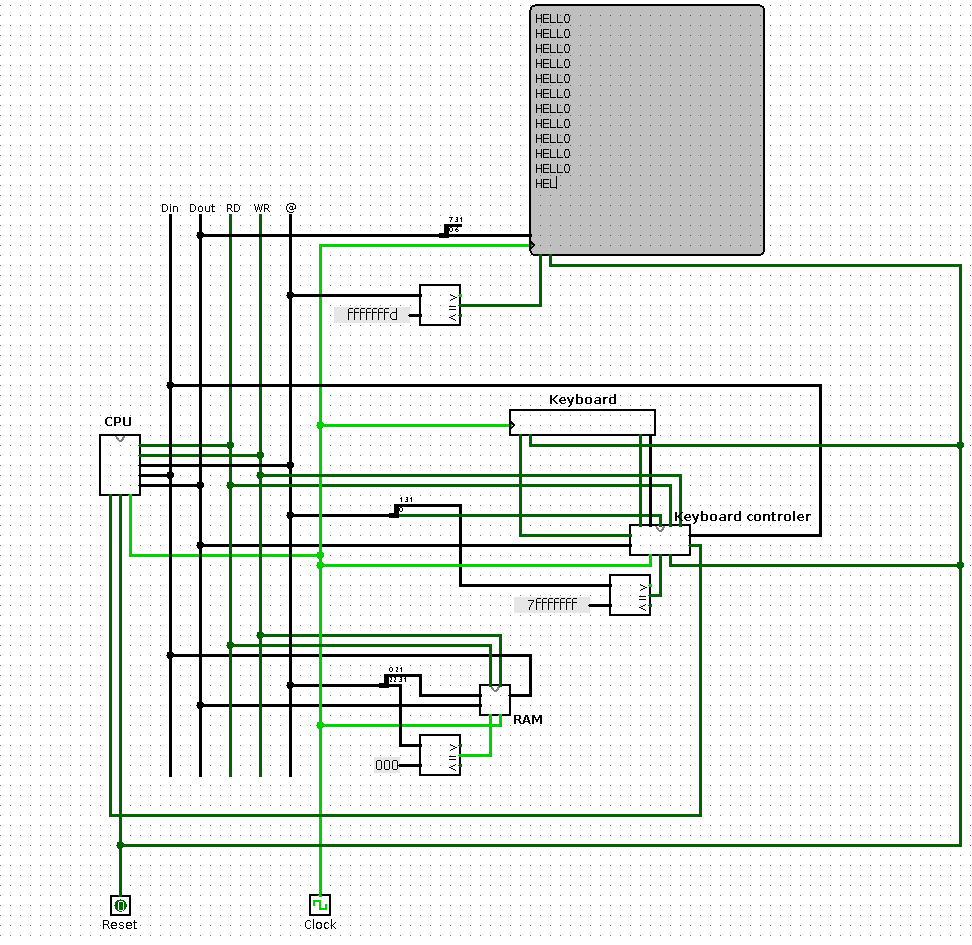
\includegraphics[width=7.2cm]{mips32_logisim.png}
\end{center}

\end{frame}

\section{Unsigned, Signed, Float}

\subsection{Unsigned}

\begin{frame}%[fragile]
\frametitle{Unsigned}

\scriptsize

\begin{itemize}

\item The range of values of an \textcolor{blue}{$n$}-bits unsigned integer is: $0$ to $2^{\textcolor{blue}{n}} - 1$.

  \begin{itemize}
    \scriptsize
  \item for $n = 8$, the maximum value is $2^{8} - 1 = 255$.
  \item for $n = 16$, the maximum value is $2^{16} - 1 = 65535$.
  \item for $n = 32$, the maximum value is $2^{32} - 1 = 4\ 294\ 967\ 295$.
  \item for $n = 64$, the maximum value is $2^{64} - 1 = 18\ 446\ 744\ 073\ 709\ 551\ 615$.\\
  \end{itemize}

  \vspace{0.4cm}

\item \texttt{C} unsigned data types\\
\end{itemize}

\begin{center}
\begin{tabular}{|c|c|c|}
    \hline
    Type & Max value (\textcolor{red}{\textbf{at least}}) & Size (in bytes) on \\
    & (as defined by the \textbf{C11} norm) & \texttt{x86-64}\\
    \hline
    \hline
    \lstinline{unsigned char} & $2^8 - 1 = 255$ & $1$ \bigstrut \\
    \hline
    \lstinline{unsigned short} & $2^{16} - 1 = 65535$ & $2$ \bigstrut\\
    \hline
    \lstinline{unsigned int} & $2^{16} - 1 = 65535$ & $4$ \bigstrut\\
    \hline
    \lstinline{unsigned long int} & $2^{32} - 1 = 4294967295$ & $8$ \bigstrut\\
    \hline
    \lstinline{unsigned long long int} & $2^{64} - 1 = 18446744073709551615$ & $8$ \bigstrut\\
    \hline
  \end{tabular}
\end{center}

\end{frame}

\begin{frame}[fragile]
\frametitle{Unsigned Addition, Substraction, Multiplication}
\scriptsize

For $n$-bits unsigned numbers, the operation ($+$, $-$, $*$) is done \textcolor{red}{modulo $2^n$}.

\vspace{0.2cm}

\begin{lstlisting}
#include <stdio.h>
int main(int argc, char *argv[]) {
  unsigned char n1 = 128;
  unsigned char n2 = 10;
  printf("%3hhu + %3hhu = %hhu\n", n1, n1, n1 + n1);
  printf("%3hhu - %3hhu = %hhu\n", n2, n1, n2 - n1);
  printf("%3hhu * %3hhu = %hhu\n", n1, n2, n1 * n2);
  printf("-%hhu = %hhu\n", n1, -n1);
  printf("  -1 = %hhu\n", -1);
  return 0;
}
// gcc -O3 unsigned.c -o unsigned && ./unsigned
// output:
//         128 + 128 = 0
//          10 - 128 = 138
//         128 *  10 = 0
//         -128 = 128
//           -1 = 255
\end{lstlisting}

\end{frame}

\begin{frame}[fragile]
\frametitle{Bit Manipulation}

\begin{itemize}

\item We can check if the $\mathbf{j}$-th bit of an integer \verb+S+ is on with\\
\begin{center}
\textcolor{blue}{\texttt{S \& (1 << j) != 0}}.
\end{center}

\vspace{0.3cm}

\item For example, if \verb+S+ $= 50$ and \verb+j+ $= 3$,
\vspace{0.1cm}

\begin{center}
\begin{Verbatim}[commandchars=@\[\]]
                         bit number
                        5|4|3|2|1|0
     50            =    1 1 @fvtextcolor[blue][0] 0 1 0
     (1 << 3)      =    0 0 @fvtextcolor[blue][1] 0 0 0
                       -------------
     50 & (1 << 3) =    0 0 @fvtextcolor[blue][0] 0 0 0
\end{Verbatim}
\end{center}

\end{itemize}

\end{frame}

\begin{frame}[fragile]
\frametitle{Bit Manipulation}

\scriptsize

\begin{itemize}

\item To turn on the $\mathbf{j}$-th bit of \verb+S+ we do: \textcolor{blue}{\texttt{S |= (1 << j)}}.

\vspace{0.1cm}

\item For example, if \verb+S+ $= 50$ and \verb+j+ $= 3$,

\begin{center}
\begin{Verbatim}[commandchars=@\[\]]
                         bit number
                        5|4|3|2|1|0
     S             =    1 1 @fvtextcolor[blue][0] 0 1 0
     (1 << 3)      =    0 0 @fvtextcolor[blue][1] 0 0 0
                       -------------
     S |= (1 << 3) =    1 1 @fvtextcolor[blue][1] 0 1 0
\end{Verbatim}
\end{center}

\vspace{0.3cm}

\item To turn off the $\mathbf{j}$-th bit of \verb+S+ we do: \textcolor{blue}{\texttt{S \&= \textasciitilde(1 << j)}}.

\vspace{0.1cm}

\item For example, if \verb+S+ $= 58$ and \verb+j+ $= 3$,

\begin{center}
\begin{Verbatim}[commandchars=@\[\]]
                          bit number
                         5|4|3|2|1|0
     S              =    1 1 @fvtextcolor[blue][1] 0 1 0
     ~(1 << 3)      =    1 1 @fvtextcolor[blue][0] 1 1 1
                        -------------
     S &= ~(1 << 3) =    1 1 @fvtextcolor[blue][0] 0 1 0
\end{Verbatim}
\end{center}

\end{itemize}

\end{frame}


\begin{frame}[fragile]
\frametitle{Bit Manipulation}

\scriptsize

\begin{itemize}

\item To toggle the $\mathbf{j}$-th bit of \verb+S+ we do: \textcolor{blue}{\texttt{S \textasciicircum= (1 << j)}}.

\vspace{0.1cm}

\item For example, if \verb+S+ $= 50$ and \verb+j+ $= 3$,

\begin{center}
\begin{Verbatim}[commandchars=@\[\]]
                         bit number
                        5|4|3|2|1|0
     S             =    1 1 @fvtextcolor[blue][0] 0 1 0
     (1 << 3)      =    0 0 @fvtextcolor[blue][1] 0 0 0
                       -------------
     S ^= (1 << 3) =    1 1 @fvtextcolor[blue][1] 0 1 0
\end{Verbatim}
\end{center}

\vspace{0.1cm}

\item For example, if \verb+S+ $= 58$ and \verb+j+ $= 3$,

\begin{center}
\begin{Verbatim}[commandchars=@\[\]]
                         bit number
                        5|4|3|2|1|0
     50            =    1 1 @fvtextcolor[blue][1] 0 1 0
     (1 << 3)      =    0 0 @fvtextcolor[blue][1] 0 0 0
                       -------------
     S ^= (1 << 3) =    1 1 @fvtextcolor[blue][0] 0 1 0
\end{Verbatim}
\end{center}

\end{itemize}

\end{frame}

\begin{frame}[fragile]
\frametitle{Bit Manipulation}

\begin{itemize}

\item To turn on all bits in a set of size $\mathbf{n}$ we do
\begin{center}
\textcolor{blue}{\texttt{(1 << n) - 1}}.
\end{center}

\vspace{0.3cm}

\item For example, if \verb+n+ $= 5$,
\vspace{0.1cm}

\begin{center}
\begin{Verbatim}[commandchars=@\[\]]
                         bit number
                        5|4|3|2|1|0
     (1 << 5)      =    1 0 0 0 0 0
            1      =    0 0 0 0 0 1
                       -------------
     (1 << 5) - 1  =    0 1 1 1 1 1
\end{Verbatim}
\end{center}

\end{itemize}

\end{frame}

\begin{frame}[fragile]
\frametitle{\exo}

\footnotesize

Write the function\\

\begin{lstlisting}
void print_subsets(const string& set)
\end{lstlisting}

which print all the subsets
of the string \lstinline{set}. Your function must be non-recursive. We suppose that \lstinline{set.size()} $\le 30$.\\

\vspace{0.3cm}

For example, \lstinline{print_subsets("abc")} gives (any order is good)

\begin{center}
\begin{verbatim}
   { }
   { a }
   { b }
   { a b }
   { c }
   { a c }
   { b c }
   { a b c }
\end{verbatim}
\end{center}

\end{frame}

\ifanswers

\begin{frame}[containsverbatim]
\frametitle{Solution Implementation}

\scriptsize

\begin{lstlisting}[mathescape]
void print_subsets(const string& set)
{
  for (unsigned int subset = 0; subset < (1U << set.size()); ++subset)
  {
    cout << "{";
    for (unsigned int j = 0; j < set.size(); ++j)
    {
      if (subset & (1 << j)) cout << " " << set[j];
    }
    cout << " }" << endl;
  }
}

int main(int argc, char *argv[])
{
  print_subsets("abc");
  return 0;
}
\end{lstlisting}

\end{frame}

\fi

\begin{frame}%[fragile]
\frametitle{Byte Ordering}

\begin{itemize}

\item Memory is byte oriented.
\vspace{0.3cm}
\item How do we store multi-bytes values?
\vspace{0.3cm}
\item Two main conventions
  \begin{itemize}
  \item Big Endian: Least significant byte has highest address (Sun, Internet for example).
    \vspace{0.1cm}
  \item Little Endian: Least significant byte has lowest address (Intel for example).
  \end{itemize}

\end{itemize}

\end{frame}

\begin{frame}%[fragile]
\frametitle{Byte Ordering}

\begin{center}
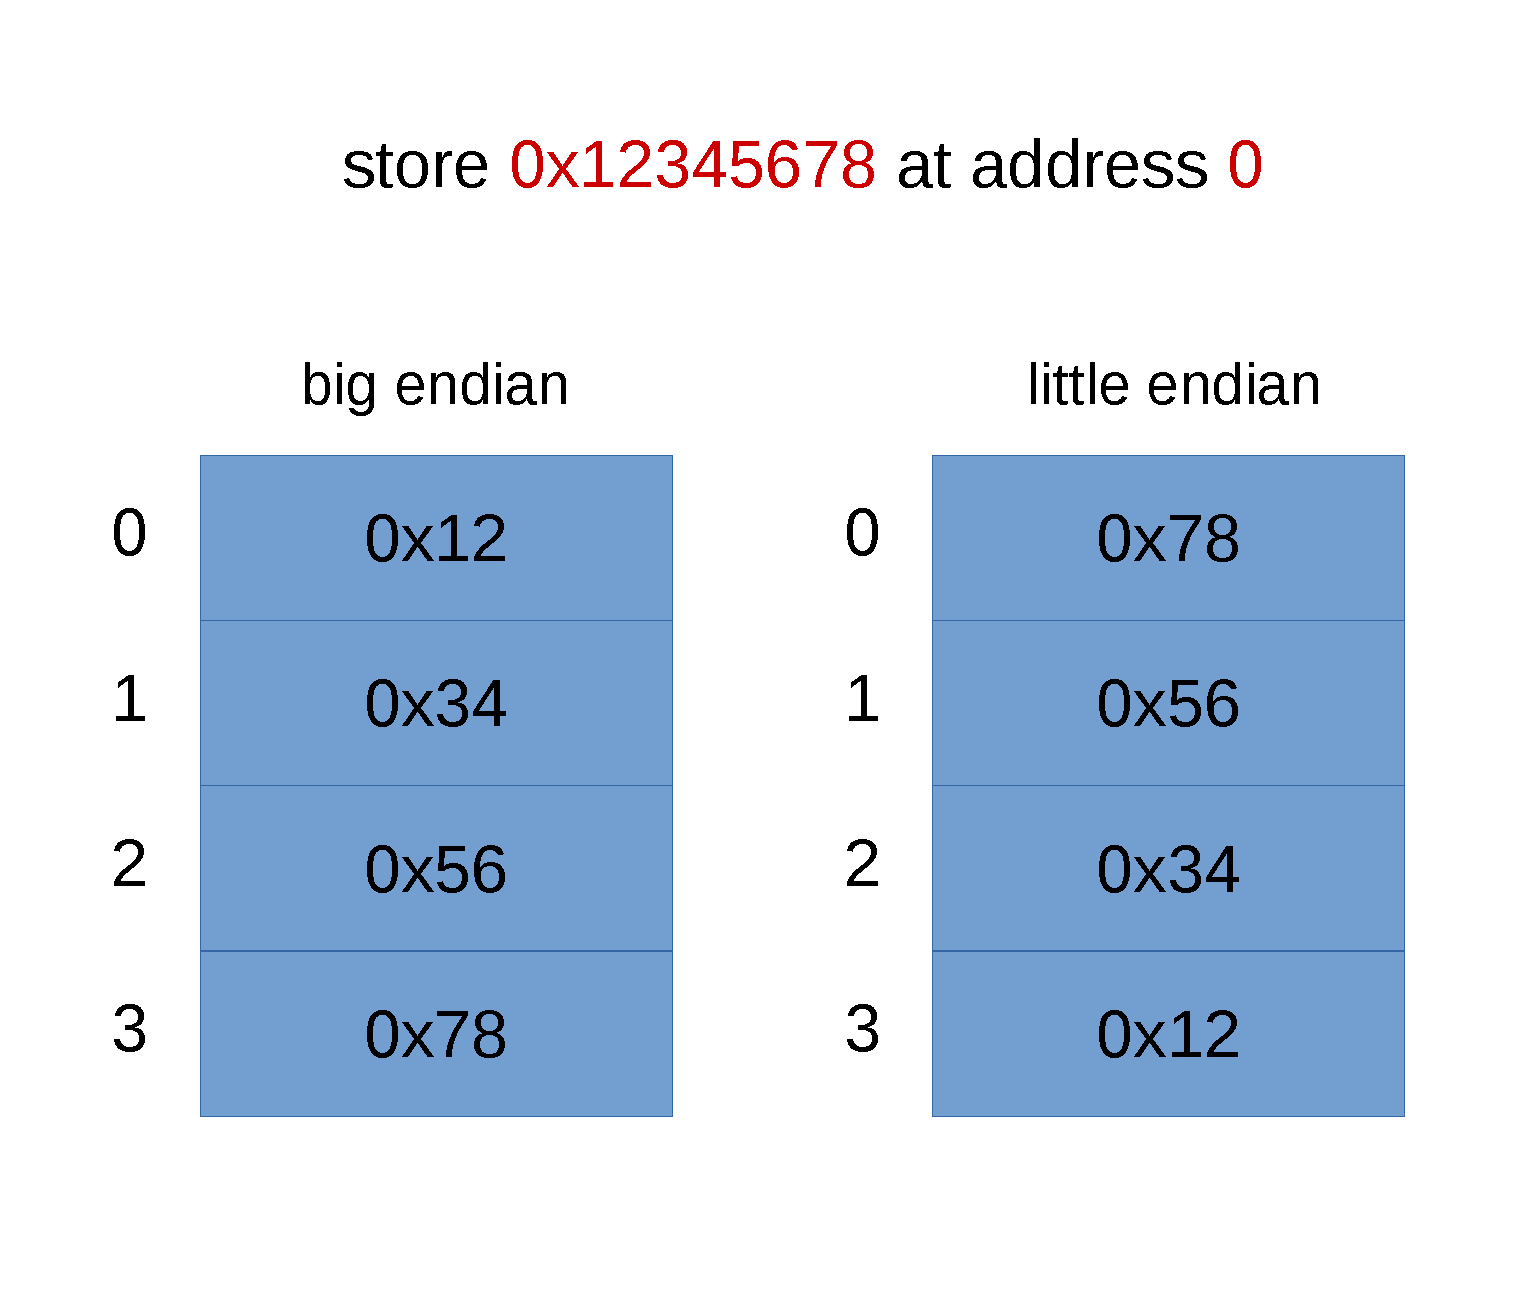
\includegraphics[width=8.5cm]{endian.pdf}
\end{center}

\end{frame}

\begin{frame}[fragile]
\frametitle{Endianness Example}
\scriptsize
\begin{lstlisting}
char chars[] = { 0, 1, 2, 3, 4, 5, 6, 7 };
int  ints[] =  { 0x00112233, 0x44556677, 0x8899aabb, 0xccddeeff };

int main() {}


// gcc endianness.c -o endianness
// objdump -sj .data endianness
// ...
// 201010 @\textcolor{red}{33221100 77665544 bbaa9988 ffeeddcc}@
// 201020 @\textcolor{red}{00010203 04050607}@
\end{lstlisting}

\end{frame}

\begin{frame}[fragile]
\frametitle{\exo}

Write a program to test the endianness of your computer.

\end{frame}

\ifanswers

\begin{frame}[fragile]
\frametitle{Solution}
\scriptsize

\begin{lstlisting}
#include <stdio.h>

int little_endian()
{
  int i = 1;
  char *p = (char *)&i;
  return p[0] == 1;
}

int main()
{
  if (little_endian())
    printf("little endian\n");
  else
    printf("big endian\n");
  return 0;
}
\end{lstlisting}

\end{frame}

\fi

\begin{frame}[fragile]
\frametitle{Looping Downward with Unsigned}

\begin{lstlisting}
unsigned int count = /* number of elements */;
for (unsigned int i = count - 2; i >= 0; --i)
{
  a[i] += a[i + 1];
}
\end{lstlisting}

\vspace{0.5cm}
Where is the bug in this code?
\end{frame}

\begin{frame}[fragile]
\frametitle{Looping Downward with Unsigned}

\begin{lstlisting}
unsigned int count = /* number of elements */;
for (unsigned int i = count - 2; i @\textcolor{red}{< count}@; --i)
{
  a[i] += a[i + 1];
}
\end{lstlisting}

\end{frame}

\subsection{Signed}

\begin{frame}%[fragile]
\frametitle{Signed}

\scriptsize

\begin{itemize}

\item Two's complement representation.

\item Let $b$ be a binary string of length $n$, the value of $b$ in the two's complement representation is
  $$
  -b_{n-1}\times2^{n-1} + \sum_{i=0}^{n - 2}b_i\times2^i
  $$

\item For example, for $n = 8$ and $b = 10010011$, we have
  $$b = -2^7 + 2^4 + 2 + 1 = -109$$

\item The range of values of an \textcolor{blue}{$n$}-bits signed integer is: $-2^{\textcolor{blue}{n-1}}$ to $2^{\textcolor{blue}{n-1}} - 1$.

  \begin{itemize}
    \scriptsize
  \item for $n = 8$, the range is $[-2^7, 2^{7} - 1] = [-128, 127]$.
  \item for $n = 16$, the range is $[-2^{15}, 2^{15} - 1] = [-32768, 32767]$.
  \item for $n = 32$, the maximum value is
    $$[-2^{31}, 2^{31} - 1] = [-2147483648, 2147483647]$$
  \item for $n = 64$, the maximum value is
    $$[-2^{63}, 2^{63} - 1] = [-9223372036854775808, 9223372036854775807]$$
  \end{itemize}

\end{itemize}

\end{frame}

\begin{frame}%[fragile]
\frametitle{\texttt{C} Language Signed Data Types}

\scriptsize

\begin{center}
\begin{tabular}{|c|c|c|}
    \hline
    Type & Range (\textcolor{red}{\textbf{at least}}) & Size (in bytes) on \\
    & (as defined by the \textbf{C11} norm) & \texttt{x86-64}\\
    \hline
    \hline
    \lstinline{char} & $[-(2^7 - 1), 2^7 - 1]$ & $1$\bigstrut\\
    \hline
    \lstinline{short} & $[-(2^{15} - 1), 2^{15} - 1]$ & $2$\bigstrut\\
    \hline
    \lstinline{int} & $[-(2^{15} - 1), 2^{15} - 1]$ & $4$\bigstrut\\
    \hline
    \lstinline{long int} & $[-(2^{31} - 1), 2^{31} - 1]$ & $8$\bigstrut\\
    \hline
    \lstinline{long long int} & $[-(2^{63} - 1), 2^{63} - 1]$ & $8$\bigstrut\\
    \hline
  \end{tabular}
\end{center}

\textbf{Note:} Even if the standard does not enforce it, compilers use two's complement (range $[-2^{n-1}, 2^{n - 1} - 1]$).

\end{frame}

\begin{frame}[fragile]
\frametitle{Signed Addition, Substraction, Multiplication and Shift}

\scriptsize

\begin{itemize}

\item Addition, substraction, multiplication and left shift are the same
operations on bit level as their unsigned counterparts.

\vspace{0.2cm}

\item Right shift propagates the sign bit.

\end{itemize}

\begin{lstlisting}
#include <stdio.h>

int main()
{
  int n1 = -1234;
  int n2 = 654321;
  int res = (int)((unsigned)n1 + (unsigned)n2);
  printf("%10d = %d\n", n1 + n2, res); //     653087 = 653087
  res = (int)((unsigned)n1 - (unsigned)n2);
  printf("%10d = %d\n", n1 - n2, res); //    -655555 = -655555
  res = (int)((unsigned)n1 * (unsigned)n2);
  printf("%10d = %d\n", n1 * n2, res); // -807432114 = -807432114
  printf("-1 >> 1 = %d\n", -1 >> 1);   // -1 >> 1 = -1
  return 0;
}
\end{lstlisting}

\end{frame}

\begin{frame}[fragile]
\frametitle{Negative Values}

\scriptsize

\begin{itemize}

\item To get the negative value of a two's complement number,
  \begin{itemize}
    \scriptsize
  \item We invert all the bits of the number.
  \item We add one to the resulting number.
  \end{itemize}

  \vspace{0.2cm}

\item Example with an $8$-bit number,
  \begin{itemize}
    \scriptsize
  \item $127 = (01111111)_2$.
  \item We invert all the bits and we get: $(10000000)_2$.
  \item Finally, we add one to get: $(10000001)_2 = -127$.
  \end{itemize}

  \vspace{0.2cm}

\item Why does it work?
  \begin{itemize}
    \scriptsize
  \item Let \textcolor{blue}{$x$} be an $8$-bit two's complement number. Let's say that \textcolor{blue}{$x = 100$}.
  \item $-\textcolor{blue}{x} = 1 + (-1 - \textcolor{blue}{x})$.
  \item All bits are set to $1$ in the two's complement representation of $-1$. So we have,
    \begin{center}
      \begin{Verbatim}[commandchars=@\[\]]
        1 1 1 1 1 1 1 1     = -1
     -  @fvtextcolor[blue][0 1 1 0 0 1 0 0]     = 100
     --------------------
        1 0 0 1 1 0 1 1     = -101
      \end{Verbatim}
    \end{center}
  \item Because all bits are set to $1$ in the two's complement representation of $-1$, the substraction flips bits in the two's complement
    representation of $x$.
  \end{itemize}

\end{itemize}

\end{frame}

\begin{frame}%[fragile]
\frametitle{Detecting Overflow}

\begin{center}
\begin{tabular}{|c|c|c|c|}
\hline
Operation & A & B & Overflow iff the result is\\
\hline
\hline
$A+B$ & $\ge 0$ & $\ge 0$ & $< 0$\\
\hline
$A+B$ & $< 0$ & $< 0$ & $\ge 0$\\
\hline
$A-B$ & $\ge 0$ & $< 0$ & $< 0$\\
\hline
$A-B$ & $< 0$ & $\ge 0$ & $\ge 0$\\
\hline
\end{tabular}

\end{center}

\end{frame}

\begin{frame}%[fragile]
\frametitle{Conversion from Signed to Unsigned}

\begin{itemize}

\item We just need to reinterpret the bit pattern.

\vspace{0.3cm}

\item If sign bit is $0$, the number is the same in both representation.

\vspace{0.3cm}

\item If sign bit is $1$, we add $2^{n}$ from signed to unsigned and substract
  $2^{n}$ from unsigned to signed.

\vspace{0.3cm}

  \begin{tabular}{|c|c|c|}
    \hline
    Bit pattern & Unsigned & Signed\\
    \hline
    \hline
    \texttt{01111111} & $127$ & $127$\\
    \hline
    \texttt{10000001} & $129$ & $129 - 2^8 = -127$\\
    \hline
    \texttt{11111111} & $-1 + 2^8 = 255$ & $-1$\\
    \hline
  \end{tabular}
\end{itemize}

\end{frame}

\begin{frame}%[fragile]
\frametitle{Conversion from Signed to Signed with Different Sizes}

\begin{itemize}

\item To convert a $n$-bits signed integer to a larger $m$-bits integer, you
  propagate the sign bit ($\textrm{bit}_{n-1}$). The value is unchanged.
  \begin{itemize}
  \item $8$-bits $\texttt{11111110} = -2$ to $16$-bits $\texttt{1111111111111110} = -2$.
  \item $8$-bits $\texttt{00000111} = 7$ to $16$-bits $\texttt{0000000000000111} = 7$.
  \end{itemize}

\vspace{0.5cm}

\item To convert a $n$-bits signed integer to a smaller $m$-bits integer, you
  cut the $(n - m)$ higher bits. The value can be changed.
  \begin{itemize}
  \item $16$-bits $\scriptsize{\texttt{1000000000000000}} = -32768$ to $8$-bits $\small{\texttt{00000000}} = 0$.
  \end{itemize}

\end{itemize}

\end{frame}

\begin{frame}[fragile]
\frametitle{Expression Containing Signed and Unsigned}

\scriptsize

If there is a mix of unsigned and signed in an expression, some conversions are applied. The \texttt{C11} norm says that
\begin{itemize}

\item ``The rank of any unsigned integer type shall equal the rank of the corresponding signed integer type, if any''.

\vspace{0.2cm}

\item ``If the operand that has unsigned integer type has rank greater than or equal to the rank of the type of the other operand, the operand with signed integer type is converted to the type of the operand with unsigned integer type''.

\end{itemize}

\vspace{0.2cm}

\begin{lstlisting}
#include <stdio.h>
int main() {
  printf("%d\n", -1 > 0U);
  // -1 is an int and 0U an unsigned int
  // output: ?
  printf("%d\n", -1L > 0U);
  // -1L is a long int and 0U an unsigned int
  // output: ?
}
\end{lstlisting}

\end{frame}

\subsection{Floating Point Numbers}

\begin{frame}%[fragile]
\frametitle{Floating Point Numbers}
\tiny
(Based on \texttt{http://www.toves.org/books/float/})
\scriptsize

\begin{itemize}
\item Based on scientific notation.

  \begin{itemize}
    \scriptsize
  \item $9.625_{(10)} = 1001.101_{(2)}$ and $1001.101_{(2)} = 1.001101 \times 2^3$ in scientific notation.
  \item $1.001101$ is called the \textcolor{blue}{\textbf{mantissa}}, and $3$ is called the \textcolor{blue}{\textbf{exponent}}.
  \end{itemize}

\item Let's illustrate the floating point encoding with an $8$-bits number.
\begin{center}
  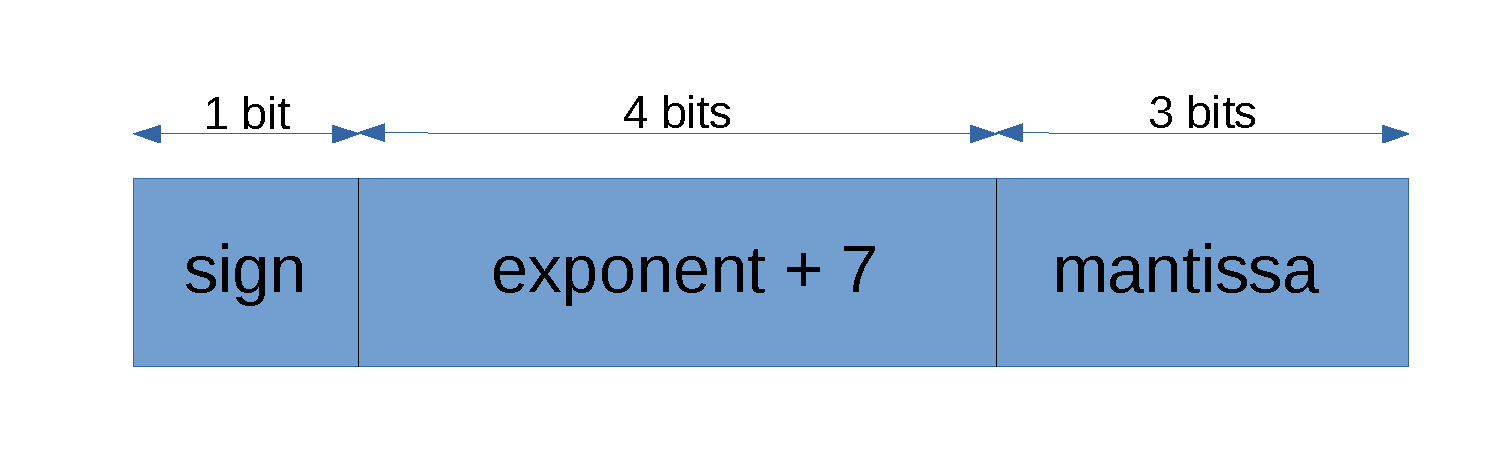
\includegraphics[width=6cm]{float1.pdf}
\end{center}

\item For $-5.5_{(10)}$ we have
  \begin{itemize}
    \scriptsize
  \item $-5.5_{(10)} = -101.1_{(2)} = -1.011\times 2^2$.
  \item We choose \texttt{1} for the \textcolor{blue}{sign bit}, because $-5.5$ is negative.
  \item We add $7$ to the exponent, we get $9_{(10)} = 1001_{(2)}$ for the \textcolor{blue}{exponent} part.
  \item The three bit of the \textcolor{blue}{mantissa} are the ones following the leading $1$. We get \texttt{011}.
  \item The final encoding is \texttt{11001011}.
  \end{itemize}

\end{itemize}

\end{frame}

\begin{frame}%[fragile]
\frametitle{\exo}

Encode \textcolor{blue}{$-0.171875$} and \textcolor{blue}{$42$} in our $8$-bits floating point format.

\end{frame}

\ifanswers
\begin{frame}%[fragile]
\frametitle{Solution}

\begin{itemize}

\item \textcolor{blue}{$-0.171875$}
  \begin{itemize}
  \item $-0.171875 = -(\frac{1}{8} + \frac{1}{32} + \frac{1}{64}) = -0.001011_{(2)}$.
  \item $-0.001011 = -1.011 \times 2^{-3}$.
  \item Final encoding: $1 0100 011$.
  \end{itemize}

\item \textcolor{blue}{$42$}
  \begin{itemize}
  \item $42 = 32 + 8 + 2 = 101010_{(2)}$.
  \item $101010 = 1.01010 \times 2^5$.
  \item We need to round to the nearest.
    \begin{itemize}
    \item But here, we have two choices: $1.010$ or $1.011$.
    \item To avoid cumulating errors, we round ties to even and so we get $1.010$.
    \end{itemize}
  \item Final encoding: $0 1100 010$.
  \end{itemize}

\end{itemize}

\end{frame}
\fi

\begin{frame}%[fragile]
\frametitle{Precision}
\tiny
(Based on \texttt{http://fabiensanglard.net/floating\_point\_visually\_explained/})

\begin{center}
  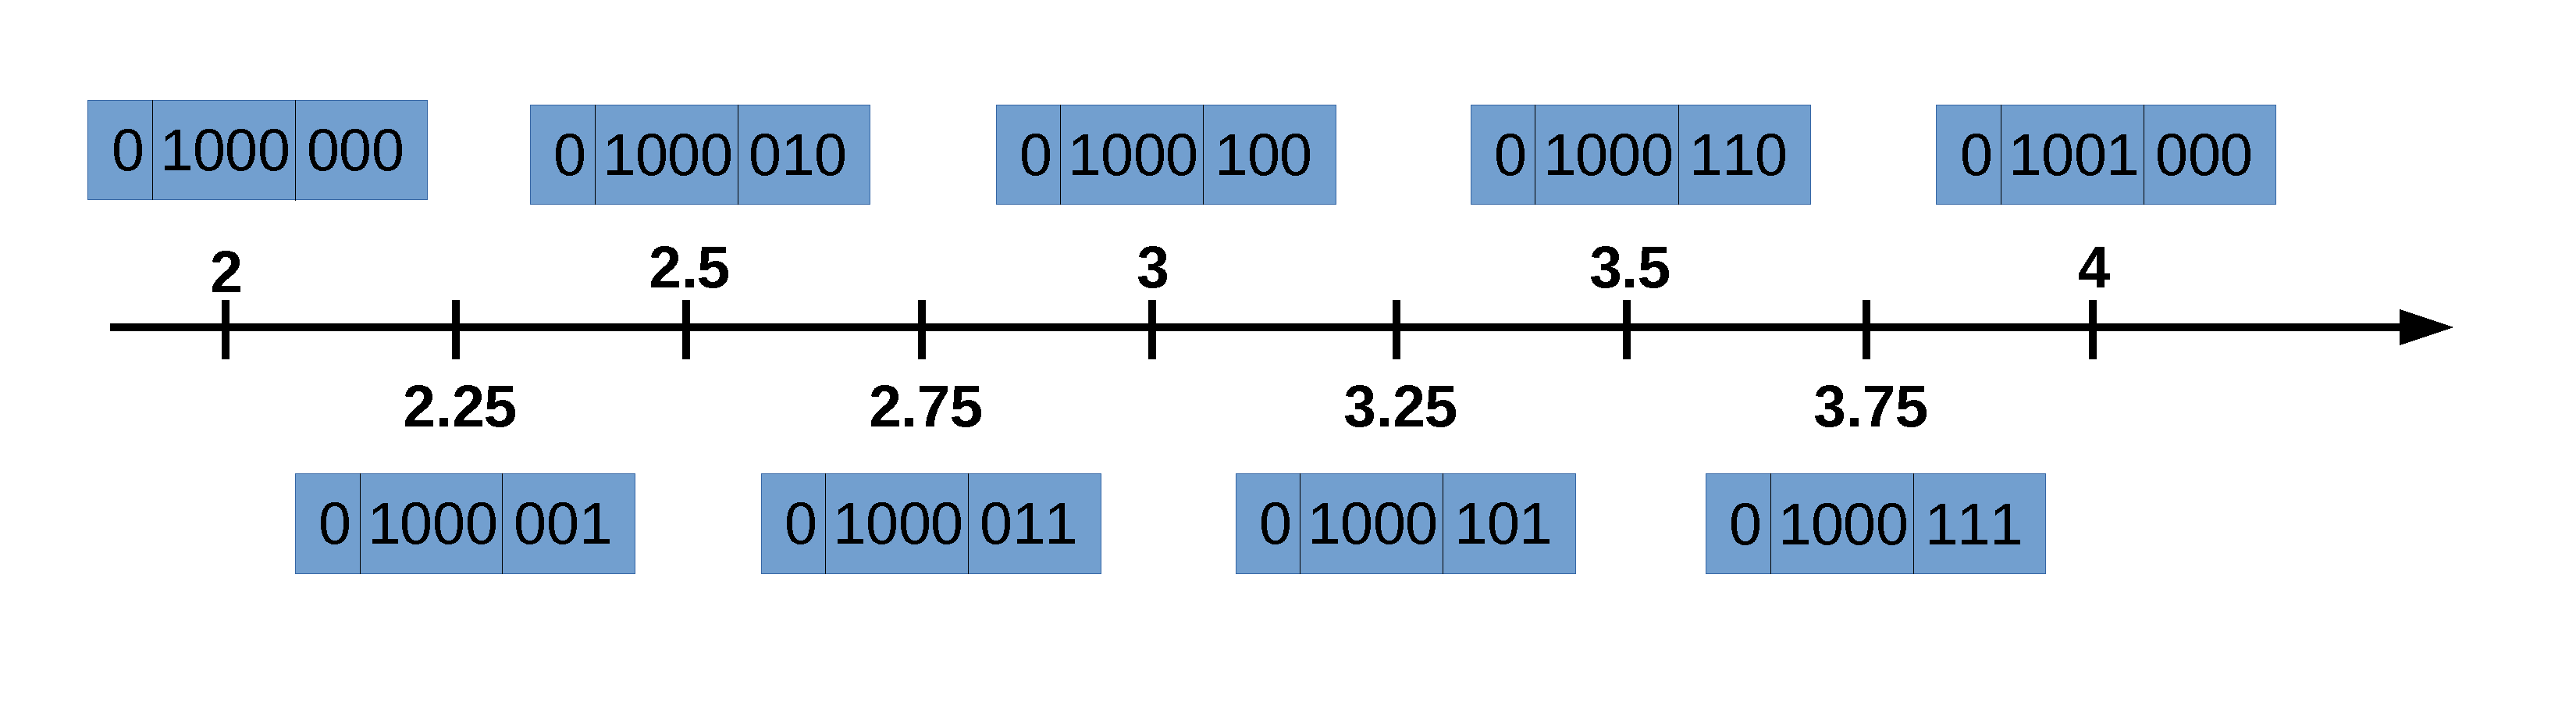
\includegraphics[width=12cm]{float2.pdf}
\end{center}

\end{frame}

\begin{frame}%[fragile]
\frametitle{Precision}

\scriptsize

\begin{itemize}

\item Consider the $8$-bits floating point numbers of the form \texttt{00110xxx}.
  \begin{itemize}
    \scriptsize
  \item The exponent is $2^{-1}$. Those numbers are in the range $[0.5, 1)$, \texttt{0\textcolor{red}{0110}000}
    to \texttt{0\textcolor{red}{0111}000}.
  \item This range is divided in $8$ steps of length $\frac{1 - 0.5}{8} = 0.0625$
    ($0.5$, $0.5625$, $0.625$, $0.6875$, $0.75$, $0.8125$, $0.875$, $0.9375$).
  \end{itemize}

\vspace{0.3cm}

\item For the $8$-bits floating point numbers of the form \texttt{01110xxx}, now we have
  \begin{itemize}
    \scriptsize
  \item The exponent is $2^{8}$. Those numbers are in the range $[128, 256)$, \texttt{0\textcolor{red}{1110}000}
    to \texttt{0\textcolor{red}{1111}000}.
  \item This range is divided in $8$ steps of length $\frac{256 - 128}{8} = 16$.
  \end{itemize}

  \vspace{0.3cm}

\item We can see that as the exponent grows, the floating points are farther apart from one another.

\end{itemize}


\end{frame}

\lstset{language=Python}

\begin{frame}[fragile]
\frametitle{Precision}

\tiny

\begin{lstlisting}
import numpy as np
import matplotlib.pyplot as plt
def sign(i):
    return -1 if i & 0x80 else 1
def exponent(i):
    return ((i & 0x78) >> 3) - 7
def mantissa(i):
    return i & 7
def to_8bit_float(i):
    return sign(i) * (1 + mantissa(i) * 0.125) * 2**exponent(i)

for i in range(0x80, 0xff + 1):
    plt.plot((to_8bit_float(i), to_8bit_float(i)), (0, 3), c='brown', linewidth=0.75, aa=False)
for i in range(0, 0x7f + 1):
    plt.plot((to_8bit_float(i), to_8bit_float(i)), (0, 3), c='blue', linewidth=0.75, aa=False)

plt.axis([-520, 520, 0, 5])
plt.xticks(np.arange(-520, 520, 40))
plt.show()
\end{lstlisting}

\begin{center}
  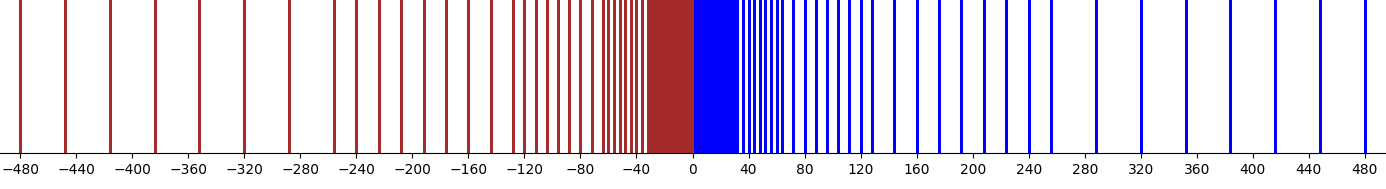
\includegraphics[width=11.5cm]{float_range1.png}
\end{center}


\end{frame}

\begin{frame}[fragile]
\frametitle{Precision}

\tiny

\begin{lstlisting}[linebackgroundcolor={\lstcolorlines{12,13,14,15,16,17,18}}]
import numpy as np
import matplotlib.pyplot as plt
def sign(i):
    return -1 if i & 0x80 else 1
def exponent(i):
    return ((i & 0x78) >> 3) - 7
def mantissa(i):
    return i & 7
def to_8bit_float(i):
    return sign(i) * (1 + mantissa(i) * 0.125) * 2**exponent(i)

for i in range(0x80, 0xdf):
    plt.plot((to_8bit_float(i), to_8bit_float(i)), (0, 3), c='brown', linewidth=0.75, aa=False)
for i in range(0, 0x5f):
    plt.plot((to_8bit_float(i), to_8bit_float(i)), (0, 3), c='blue', linewidth=0.75, aa=False)

plt.axis([-2.25, 2.25, 0, 5])
plt.xticks(np.arange(-2.25, 2.25, 0.25))
plt.show()
\end{lstlisting}

\begin{center}
  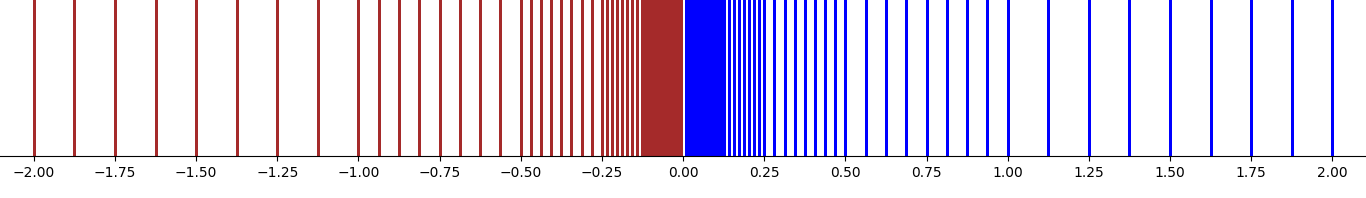
\includegraphics[width=11.5cm]{float_range2.png}
\end{center}

\end{frame}


\begin{frame}[fragile]
\frametitle{Precision}

\tiny

\begin{lstlisting}
# ...
for i in range(0x80, 0x8f):
    plt.plot((to_8bit_float(i), to_8bit_float(i)), (0, 3), c='brown', linewidth=0.75, aa=False)
for i in range(0, 0x0f):
    plt.plot((to_8bit_float(i), to_8bit_float(i)), (0, 3), c='blue', linewidth=0.75, aa=False)

plt.axis([-0.03, 0.03, 0, 5])
plt.xticks(np.arange(-0.02734375, 0.027348, 2**-8))
locs, _ = plt.xticks()
labels = ['%.8f' % v for v in locs]
plt.xticks(locs, labels)

plt.show()
\end{lstlisting}

\begin{center}
  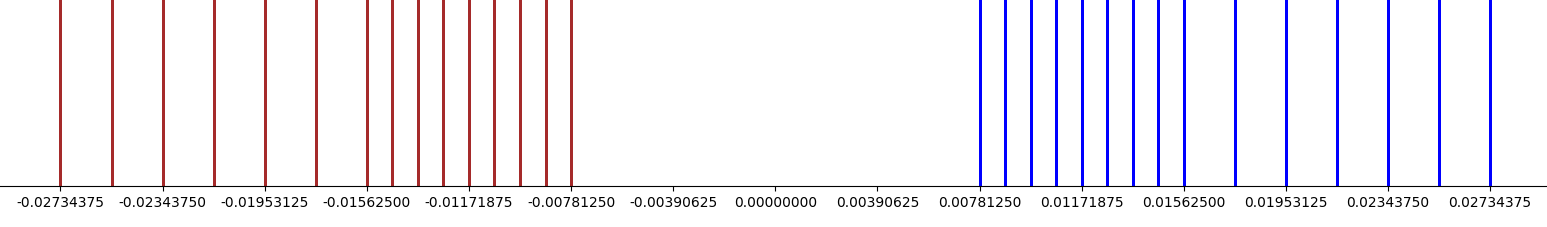
\includegraphics[width=11.5cm]{float_near_zero1.png}
\end{center}

\scriptsize

There's a large gap between $-0.0078125$ and $0.0078125$ and we can't represent zero!

\end{frame}

\begin{frame}[fragile]
\frametitle{Denormalized Floating Point Numbers}

\begin{itemize}

\item When the exponent is $0$, the number is in denormalized form and,
\begin{itemize}
\item We only subtract $6$ and not $7$.
\item The mantissa is not un its normal form, the $1$ to the left of the decimal point
  is replaced by a $0$.
\end{itemize}

\vspace{0.3cm}

\item We use $-6$ for the exponent, to make a smooth transition with the normalized numbers.
  \begin{itemize}
  \item The smallest positive normalized number is \textcolor{blue}{\texttt{0\textcolor{red}{0001}000}} which is $2^{-6} = 0.015625$.
  \item The biggest positive normalized number is \textcolor{blue}{\texttt{0\textcolor{red}{0000}111}} which is $2^{-6} \times (0.5 + 0.25 + 0.125) = 0.013671875$.
  \end{itemize}

  \vspace{0.3cm}

\item We have two zeroes, \textcolor{blue}{\texttt{00000000}} ($0$) and \textcolor{blue}{\texttt{10000000}} ($-0$).

\end{itemize}

\end{frame}


\begin{frame}[fragile]
\frametitle{Denormalized Floating Point Numbers}
\tiny

\begin{lstlisting}[linebackgroundcolor={\lstcolorlines{5,6,7,8,9,10,13,14,15}}]
import numpy as np
import matplotlib.pyplot as plt
def sign(i):
    return -1 if i & 0x80 else 1
def exponent(i):
    e = (i & 0x78) >> 3
    if e == 0:
        return -6, True
    else:
        return e - 7, False
def mantissa(i):
    return i & 7
def to_8bit_float(i):
    e, denormalized = exponent(i)
    return sign(i) * ((0 if denormalized else 1) + mantissa(i) * 0.125) * 2**e
n = 20
for i in range(0x80, 0x8f):
    plt.plot((to_8bit_float(i), to_8bit_float(i)), (0, 3), c='brown', linewidth=0.75, aa=False)
for i in range(0, 0x0f):
    plt.plot((to_8bit_float(i), to_8bit_float(i)), (0, 3), c='blue', linewidth=0.75, aa=False)
plt.axis([-0.03, 0.03, 0, 5])
plt.xticks(np.arange(-0.02734375, 0.027348, 2**-8))
locs, _ = plt.xticks()
labels = ['%.8f' % v for v in locs]
plt.xticks(locs, labels)
plt.show()
\end{lstlisting}

\end{frame}


\begin{frame}%[fragile]
\frametitle{Denormalized Floating Point Numbers}

\begin{center}
  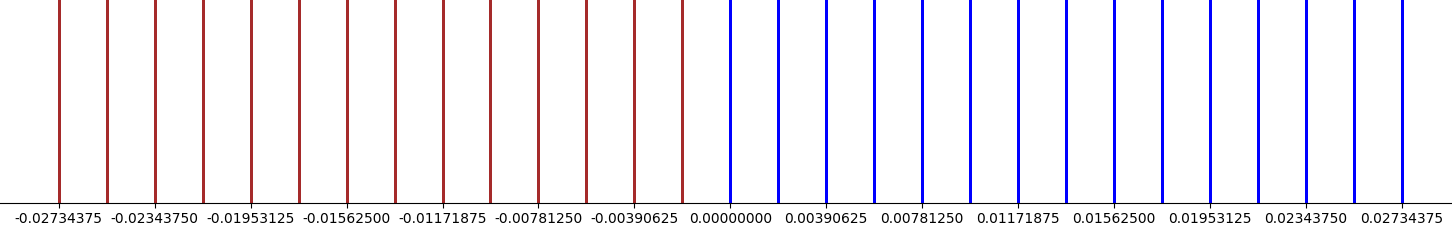
\includegraphics[width=11.5cm]{denormalized.png}
\end{center}

\end{frame}

\begin{frame}%[fragile]
\frametitle{Special Floating Point Numbers}

\begin{itemize}

\item If the exponent is all ones and the mantissa is all zeroes, then the number represents infinity or negative infinity, depending on the sign bit.
  This value results from an overflow. For example,
  \begin{itemize}
  \item \lstinline+float v = 1.0 / pow(2, -128);+
  \item \lstinline+float v = pow(2, 128);+
  \item $1.0 / 0.0$.
  \end{itemize}

\vspace{0.5cm}

\item If the exponent is all ones, and the mantissa has some non-zero bits, then the number represents ``not a number'', written as \texttt{NaN}.
  For example,
  \begin{itemize}
  \item $0.0 / 0.0$.
  \item $\infty - \infty$.
  \item $\infty / \infty$.
  \end{itemize}

\end{itemize}

\end{frame}

\begin{frame}%[fragile]
\frametitle{IEEE 754 Format}

\begin{tabular}{|l|c|c|c|c|c|}
  \hline
  Format & sign & exponent & mantissa & exponent excess\\
  \hline
  \hline
  Our $8$-bit & 1 & 4 & 3 & 7\\
  \hline
  IEEE $32$-bit & 1 & 8 & 23 & 127\\
  \hline
  IEEE $64$-bit & 1 & 11 & 52 & 1023\\
  \hline
  IEEE $128$-bit & 1 & 15 & 112 & 16383\\
  \hline
\end{tabular}

\end{frame}

\begin{frame}%[fragile]
\frametitle{\exo}

\begin{enumerate}
\item What's the biggest number (different from $\infty$) we can represent with the IEEE $64$-bit format?
  \vspace{0.5cm}
\item What's the smallest positive number we can represent with the IEEE $64$-bit format?
\end{enumerate}

\end{frame}

\ifanswers
\begin{frame}%[fragile]
\frametitle{Solution}

\scriptsize

\begin{enumerate}
\item The biggest number is\\
  \vspace{0.2cm}
  \begin{tabular}{|c|c|c|}
    \hline
    0 & 11111111110 & 1111111111111111111111111111111111111111111111111111\\
    \hline
  \end{tabular}
  $$
  \begin{array}{l l}
    = & 2^{2046 - 1023}\times(\sum_{i = 0}^{52} 2^{-i})\\
    = & 2^{1023}\times\frac{1-2^{-53}}{1-2^{-1}}\\
    \simeq & 1.79769313486232\mathrm{e}{+308}\\
  \end{array}
  $$
\item The smallest positive number is\\
    \vspace{0.2cm}
  \begin{tabular}{|c|c|c|}
    \hline
    0 & 00000000000 & 0000000000000000000000000000000000000000000000000001\\
    \hline
  \end{tabular}
  $$
  \begin{array}{l l}
    = & 2^{-1022}\times 2^{-52}\\
    \simeq & 4.94065645841247\mathrm{e}{-324}\\
  \end{array}
  $$
\end{enumerate}

\end{frame}
\fi

%% \begin{frame}%[fragile]
%% \frametitle{Floating Point Multiplication}


%% \end{frame}


\begin{frame}%[fragile]
\frametitle{Floating Point Addition}
\tiny
(From \texttt{David Goldberg, Computer Arithmetic})
\vspace{0.5cm}

\scriptsize

Let $a_1$ and $a_2$ be the two numbers to be added. The notations $e_i$
and $s_i$ are used for the exponent and significand of the addends $a_i$.
This means that the floating-point inputs have been unpacked and that $s_i$
has an explicit leading bit. To add $a_1$ and $a_2$, perform these eight steps:

\begin{enumerate}

\item If $e_1 < e_2$ swap the operands. This ensures that the difference of the exponents
  satisfies $d = e_1 - e_2 \ge 0$. Tentatively, set the exponent of the result to $e_1$.\\

\item If the signs of $a_1$ and $a_2$ differ, replace $s_2$ by its two's complement.\\

\item Place $s_2$ in a $p$-bit register (where $p$ is the number of bits of $s_2$)
  and shift it $d = e_1 - e2$ places to the right (shifting in
1's if $s_2$ was complemented in the previous step). From the bits shifted out, set $g$ (guard)
to the most-significant bit, set $r$ (round) to the next most-significant bit, and set $s$ (sticky) to
the OR of the rest.

\item Compute a preliminary significand $S = s_1 + s_2$ by adding $s_1$ to the $p$-bit register
containing $s_2$. If the signs of $a_1$ and $a_2$ are different, the most-significant bit of $S$
is $1$, and there was no carry-out, then $S$ is negative. Replace $S$ with its two's
complement. This can only happen when $d = 0$.

\end{enumerate}

\end{frame}

\begin{frame}%[fragile]
\frametitle{Floating Point Addition}

\scriptsize

\begin{enumerate}
\setcounter{enumi}{4}
\item Shift $S$ as follows. If the signs of $a_1$ and $a_2$ are the same and there was a carryout
  in step 4, shift $S$ right by one, filling in the high-order position with 1 (the carry-out).
  Otherwise, shift it left until it is normalized. When left-shifting, on the first
shift fill in the low-order position with the $g$ bit. After that, shift in zeros. Adjust
the exponent of the result accordingly.

\item Adjust $r$ and $s$. If $S$ was shifted right in step 5, set $s := g \vee r \vee s$ and set $r :=$ low-order bit of $S$ before
  shifting. If there was no shift, set $r := g$, $s := r \vee s$.
  If there was a single left shift, don't change $r$ and $s$. If there were two or more left
shifts, $r := 0$, $s := 0$.

\item Round $S$: Let $p_0$ the low order bit of $S$. Add $1$ to $S$ iff $((r \wedge p_0) \vee (r \wedge s))$.
  If rounding causes carry-out, shift $S$ right and adjust the exponent. This is the significand of the result.

\item Compute the sign of the result with the following table, where the \emph{swap} column refers to swapping the operands
  in step 1, while the \emph{compl} column refers to performing a two's complement in step 4, Blanks are ``don't care'':
  \tiny
%  \vspace{0.15cm}
  \begin{center}
  \begin{tabular}{|c|c|c|c|c|}
    \hline
    \textbf{swap} & \textbf{compl} & \textbf{sign($a_1$)} & \textbf{sign($a_2$)} & \textbf{sign(result)}\\
    \hline
        &     & s & s & s\\
    Yes &     & + & - & -\\
    Yes &     & - & + & +\\
    No  & No  & + & - & +\\
    No  & No  & - & + & -\\
    No  & Yes & + & - & -\\
    No  & Yes & - & + & +\\
    \hline
  \end{tabular}
  \end{center}
\end{enumerate}

\end{frame}

\begin{frame}[fragile]
\frametitle{Floating Point Addition Example}

\scriptsize

We follow the preeceding algorithm to compute the sum
$$
\textcolor{blue}{(-1.001_2\times 2^{-2}) + (-1.111_2\times 2^{0})}.
$$
We have $s_1 = 1.001$, $e_1 = -2$, $s_2 = 1.111$ and $e_2 = 0$.\\

\begin{enumerate}

\item $e_1 < e_2$ so swap, $d = 2$, tentative $exp = 0$.\\

\item Signs of both operands negative, don't negate $s_2$.\\

\item Shift $s2$ ($1.001$ after swap) right by $d = 2$, giving $s_2 = 0.010$, $g = 0$, $r = 1$, $s = 0$.\\

\item
  \begin{center}
    \begin{Verbatim}[commandchars=@\[\]]
        1.111
     +  0.010
      --------
     (1)0.001
    \end{Verbatim}
  \end{center} $S = 0.001$, with a carry-out.\\

\item Carry-out, so shift $S$ right, $S = 1.000$, $exp := exp + 1 = 1$.\\

\item $s := g \vee r \vee s = 0 \vee 1 \vee 0 = 1$. $r =$ low order bit of sum $= 1$.\\

\item $r \wedge s = true$, so round up, $S := S + 1 = 1.001$.\\

\item Both signs are negative, so sign of result is negative. Final result: $\textcolor{blue}{-1.001_2\times 2^1}$.

\end{enumerate}

\end{frame}

\begin{frame}[fragile]
\frametitle{Floating Point Addition Example}

\scriptsize

We follow the preeceding algorithm to compute the sum
$$
\textcolor{blue}{-1.010_2 + 1.100_2}.
$$
We have $s_1 = 1.010$, $e_1 = 0$, $s_2 = 1.100$ and $e_2 = 0$.\\

\begin{enumerate}

\item No swap, $d = 0$, tentative $exp = 0$.\\

\item Signs differ, replace $s_2$ with $0.100$ (two's complement of $1.100$).\\

\item $d = 0$ so no shift. $g = r = s = 0$.\\

\item
  \begin{center}
    \begin{Verbatim}[commandchars=@\[\]]
        1.010
     +  0.100
      --------
        1.110
    \end{Verbatim}
  \end{center} Signs are different, most-significant bit is $1$, no carry-out, so must two's complement sum, giving $S = 0.010$.\\

\item Shift left twice, so $S = 1.000$, $exp := exp - 2 = -2$.\\

\item Two left shifts, so $r = g = s = 0$.\\

\item No addition required for rounding.\\

\item Final result is $sign \times S\times 2^{exp}$ or $sign \times 1.000 \times 2^{-2}$.
  Since complement but no swap and $sign(a_1)$ is $-$, the sign of the sum is $+$.
  Final result: $\textcolor{blue}{1.000_2\times 2^{-2}}$.

\end{enumerate}

\end{frame}

\lstset{language = c++, frameround = fttt, frame=trBL}

\begin{frame}[fragile]
\frametitle{\exo}

Compute the addition: \lstinline{100'000'001 + 1}.\\
Then, show why the following \lstinline{for} loops forever.\\
\vspace{0.5cm}
\scriptsize
\begin{lstlisting}
int main(int argc, char *argv[])
{
  for (float x = 100'000'001; x <= 100'000'010; x += 1.0)
    {
    }
  return 0;
}
\end{lstlisting}

\end{frame}


\section{From C to Binary}

\begin{frame}[fragile]
\frametitle{From C to Binary}

\scriptsize

\begin{itemize}

\item We have three files: \texttt{\textcolor{blue}{maths.h}}, \texttt{\textcolor{blue}{maths.c}} and \texttt{\textcolor{blue}{main.c}}

  \vspace{0.5cm}

\item We create two object files, \texttt{\textcolor{blue}{maths.o}} and \texttt{\textcolor{blue}{main.o}} with
  \begin{Verbatim}
    $ gcc -c maths.c
    $ gcc -c main.c
  \end{Verbatim}

  \vspace{0.5cm}

\item We link these two object files into an executable \texttt{\textcolor{blue}{main}} with
  \begin{Verbatim}
    $ gcc maths.o main.o -o main
  \end{Verbatim}
  \vspace{0.5cm}

\item We execute it with
    \begin{Verbatim}
      $ ./main
    \end{Verbatim}
  \vspace{0.1cm}

    and the \texttt{\textcolor{blue}{shell}} will call the \texttt{\textcolor{blue}{execve}} system call to ask the linux kernel to
    execute it. You can see this with
    \begin{Verbatim}
      $ strace ./main
      execve("./main", ["./main"], 0x7ffeba26bf70 /* 62 vars */) = 0
      ...
    \end{Verbatim}

\end{itemize}

\end{frame}

\lstset{language = c++, frameround = fttt, frame=trBL}

\begin{frame}[fragile]
\frametitle{Header File}
\scriptsize
\begin{lstlisting}
// maths.h
#pragma once

extern double PI;

int gcd(int a, int b);

long factorial(int n);
\end{lstlisting}

\end{frame}

\begin{frame}[fragile]
\frametitle{Source File}
\scriptsize
\begin{lstlisting}
// maths.c
#include "maths.h"

double PI = 3.141592653589793;

int gcd(int a, int b)
{
  return b == 0 ? a : gcd(b, a % b);
}

long factorial(int n)
{
  if (n < 2) return 1;
  return n * factorial(n - 1);
}

\end{lstlisting}

\end{frame}

\begin{frame}[fragile]
\frametitle{Main Source File}
\scriptsize
\begin{lstlisting}
// main.c
#include <stdio.h>
#include "maths.h"

int main(int argc, char *argv[])
{
  long f = factorial(25);
  int g = gcd(24, 42);
  printf("f = %ld, g = %d, PI = %.8lf\n", f, g, PI);
  return 0;
}
\end{lstlisting}

\end{frame}

\begin{frame}[fragile]
\frametitle{Preprocessing}
\scriptsize
\begin{verbatim}
$ gcc -H -c main.c
\end{verbatim}
\tiny
\begin{verbatim}
. /usr/include/stdio.h
.. /usr/include/x86_64-linux-gnu/bits/libc-header-start.h
... /usr/include/features.h
.... /usr/include/x86_64-linux-gnu/sys/cdefs.h
..... /usr/include/x86_64-linux-gnu/bits/wordsize.h
..... /usr/include/x86_64-linux-gnu/bits/long-double.h
.... /usr/include/x86_64-linux-gnu/gnu/stubs.h
..... /usr/include/x86_64-linux-gnu/gnu/stubs-64.h
.. /usr/lib/gcc/x86_64-linux-gnu/7/include/stddef.h
.. /usr/include/x86_64-linux-gnu/bits/types.h
... /usr/include/x86_64-linux-gnu/bits/wordsize.h
... /usr/include/x86_64-linux-gnu/bits/typesizes.h
.. /usr/include/x86_64-linux-gnu/bits/types/__FILE.h
.. /usr/include/x86_64-linux-gnu/bits/types/FILE.h
.. /usr/include/x86_64-linux-gnu/bits/libio.h
... /usr/include/x86_64-linux-gnu/bits/_G_config.h
.... /usr/lib/gcc/x86_64-linux-gnu/7/include/stddef.h
.... /usr/include/x86_64-linux-gnu/bits/types/__mbstate_t.h
... /usr/lib/gcc/x86_64-linux-gnu/7/include/stdarg.h
.. /usr/include/x86_64-linux-gnu/bits/stdio_lim.h
.. /usr/include/x86_64-linux-gnu/bits/sys_errlist.h
. maths.h
\end{verbatim}

\end{frame}

\begin{frame}[fragile]
\frametitle{Object Files}
\tiny
\begin{verbatim}
$ gcc -c maths.c
$ objdump -dr maths.o
\end{verbatim}
\begin{lstlisting}[numbers=none]
maths.o:     @\textcolor{red}{file format elf64-x86-64}@
Disassembly of section .text:

0000000000000037 <gcd>:
  37:	55                      push   %rbp
  38:	48 89 e5                mov    %rsp,%rbp
  3b:	48 83 ec 10             sub    $0x10,%rsp
  3f:	89 7d fc                mov    %edi,-0x4(%rbp)
  42:	89 75 f8                mov    %esi,-0x8(%rbp)
  45:	83 7d f8 00             cmpl   $0x0,-0x8(%rbp)
  49:	74 15                   je     60 <gcd+0x29>
  4b:	8b 45 fc                mov    -0x4(%rbp),%eax
  4e:	99                      cltd
  4f:	f7 7d f8                idivl  -0x8(%rbp)
  52:	8b 45 f8                mov    -0x8(%rbp),%eax
  55:	89 d6                   mov    %edx,%esi
  57:	89 c7                   mov    %eax,%edi
  59:	e8 @\textcolor{red}{00 00 00 00}@          callq  5e <gcd+0x27>
                        @\textcolor{red}{5a: R\_X86\_64\_PC32}@	gcd-0x4
  5e:	eb 03                   jmp    63 <gcd+0x2c>
  60:	8b 45 fc                mov    -0x4(%rbp),%eax
  63:	c9                      leaveq
  64:	c3                      retq
\end{lstlisting}

\end{frame}

\begin{frame}[fragile]
\frametitle{Object Files}
\tiny
\begin{lstlisting}[numbers=none]
0000000000000000 <factorial>:
   0:	55                      push   %rbp
   1:	48 89 e5                mov    %rsp,%rbp
   4:	53                      push   %rbx
   5:	48 83 ec 18             sub    $0x18,%rsp
   9:	89 7d ec                mov    %edi,-0x14(%rbp)
   c:	83 7d ec 01             cmpl   $0x1,-0x14(%rbp)
  10:	7f 07                   jg     19 <factorial+0x19>
  12:	b8 01 00 00 00          mov    $0x1,%eax
  17:	eb 17                   jmp    30 <factorial+0x30>
  19:	8b 45 ec                mov    -0x14(%rbp),%eax
  1c:	48 63 d8                movslq %eax,%rbx
  1f:	8b 45 ec                mov    -0x14(%rbp),%eax
  22:	83 e8 01                sub    $0x1,%eax
  25:	89 c7                   mov    %eax,%edi
  27:	e8 @\textcolor{red}{00 00 00 00}@          callq  2c <factorial+0x2c>
                        @\textcolor{red}{28: R\_X86\_64\_PC32}@	factorial-0x4
  2c:	48 0f af c3             imul   %rbx,%rax
  30:	48 83 c4 18             add    $0x18,%rsp
  34:	5b                      pop    %rbx
  35:	5d                      pop    %rbp
  36:	c3                      retq
\end{lstlisting}

\end{frame}

\begin{frame}[fragile]
\frametitle{Object Files}
\scriptsize
\begin{verbatim}
$ objdump -sj .data maths.o
\end{verbatim}

\begin{lstlisting}[numbers=none]
maths.o:     file format elf64-x86-64

Contents of section .data:
 0000 @\textcolor{red}{182d4454 fb210940}@
\end{lstlisting}
\end{frame}

\begin{frame}[fragile]
\frametitle{Object Files}
\scriptsize
\begin{verbatim}
$ gcc -c main.c
$ objdump -dr main.o
\end{verbatim}
\tiny
\begin{lstlisting}[numbers=none]
main.o:     file format elf64-x86-64

Disassembly of section .text:

0000000000000000 <main>:
   0:   55                      push   %rbp
   1:   48 89 e5                mov    %rsp,%rbp
   4:   48 83 ec 30             sub    $0x30,%rsp
   8:   89 7d ec                mov    %edi,-0x14(%rbp)
   b:   48 89 75 e0             mov    %rsi,-0x20(%rbp)
   f:   bf 19 00 00 00          mov    $0x19,%edi
  14:   e8 @\textcolor{red}{00 00 00 00}@          callq  19 <main+0x19>
                        @\textcolor{red}{15: R\_X86\_64\_PLT32}@      factorial-0x4
  19:   48 89 45 f8             mov    %rax,-0x8(%rbp)
  1d:   be 2a 00 00 00          mov    $0x2a,%esi
  22:   bf 18 00 00 00          mov    $0x18,%edi
  27:   e8 @\textcolor{red}{00 00 00 00}@          callq  2c <main+0x2c>
                        @\textcolor{red}{28: R\_X86\_64\_PLT32}@      gcd-0x4
\end{lstlisting}


\end{frame}

\begin{frame}[fragile]
\frametitle{Object Files}
\tiny
\begin{lstlisting}[numbers=none]
  2c:   89 45 f4                mov    %eax,-0xc(%rbp)
  2f:   48 8b 0d @\textcolor{red}{00 00 00 00}@    mov    0x0(%rip),%rcx        # 36 <main+0x36>
                        @\textcolor{red}{32: R\_X86\_64\_PC32}@       PI-0x4
  36:   8b 55 f4                mov    -0xc(%rbp),%edx
  39:   48 8b 45 f8             mov    -0x8(%rbp),%rax
  3d:   48 89 4d d8             mov    %rcx,-0x28(%rbp)
  41:   f2 0f 10 45 d8          movsd  -0x28(%rbp),%xmm0
  46:   48 89 c6                mov    %rax,%rsi
  49:   48 8d 3d @\textcolor{red}{00 00 00 00}@    lea    0x0(%rip),%rdi        # 50 <main+0x50>
                        @\textcolor{red}{4c: R\_X86\_64\_PC32}@       .rodata-0x4
  50:   b8 01 00 00 00          mov    $0x1,%eax
  55:   e8 @\textcolor{red}{00 00 00 00}@          callq  5a <main+0x5a>
                        @\textcolor{red}{56: R\_X86\_64\_PLT32}@      printf-0x4
  5a:   b8 00 00 00 00          mov    $0x0,%eax
  5f:   c9                      leaveq
  60:   c3                      retq
\end{lstlisting}

\end{frame}

\begin{frame}[fragile]
\frametitle{Object Files}
\scriptsize
\begin{verbatim}
$ objdump -sj .rodata main.o
\end{verbatim}

\begin{lstlisting}[numbers=none]
main.o:     file format elf64-x86-64

Contents of section .rodata:
 0000 @\textcolor{red}{66203d20 256c642c 2067203d 2025642c}@  f = %ld, g = %d,
 0010 @\textcolor{red}{20504920 3d20252e 386c660a 00}@         PI = %.8lf..
\end{lstlisting}

\end{frame}

\begin{frame}[fragile]
\frametitle{Executable File}
\tiny
\begin{verbatim}
$ gcc maths.o main.o -o main && objdump -dr main
\end{verbatim}
\vspace{-0.2cm}
\begin{lstlisting}[numbers=none, escapechar={~}]
00000000000006af <main>:
 6af:   55                      push   %rbp
 6b0:   48 89 e5                mov    %rsp,%rbp
 6b3:   48 83 ec 30             sub    $0x30,%rsp
 6b7:   89 7d ec                mov    %edi,-0x14(%rbp)
 6ba:   48 89 75 e0             mov    %rsi,-0x20(%rbp)
 6be:   bf 19 00 00 00          mov    $0x19,%edi
 6c3:   e8 ~\textcolor{red}{82 ff ff ff}~          callq  ~\textcolor{red}{64a}~ <factorial>
 6c8:   48 89 45 f8             mov    %rax,-0x8(%rbp)
 6cc:   be 2a 00 00 00          mov    $0x2a,%esi
 6d1:   bf 18 00 00 00          mov    $0x18,%edi
 6d6:   e8 ~\textcolor{red}{a6 ff ff ff}~          callq  ~\textcolor{red}{681}~ <gcd>
 6db:   89 45 f4                mov    %eax,-0xc(%rbp)
 6de:   48 8b ~\textcolor{red}{0d 2b 09 20 00}~    mov    ~\textcolor{red}{0x20092b(\%rip),\%rcx}~    # 201010 <PI>
 6e5:   8b 55 f4                mov    -0xc(%rbp),%edx
 6e8:   48 8b 45 f8             mov    -0x8(%rbp),%rax
 6ec:   48 89 4d d8             mov    %rcx,-0x28(%rbp)
 6f0:   f2 0f 10 45 d8          movsd  -0x28(%rbp),%xmm0
 6f5:   48 89 c6                mov    %rax,%rsi
 6f8:   48 8d 3d 95 00 00 00    lea    0x95(%rip),%rdi        # 794 <_IO_stdin_used+0x4>
 6ff:   b8 01 00 00 00          mov    $0x1,%eax
 704:   e8 ~\textcolor{red}{17 fe ff ff}~          callq  ~\textcolor{red}{520}~ <printf@plt>
 709:   b8 00 00 00 00          mov    $0x0,%eax
 70e:   c9                      leaveq
 70f:   c3                      retq
\end{lstlisting}

\end{frame}

\begin{frame}[fragile]
\frametitle{Memory Mapping}
\tiny
\begin{lstlisting}[language = pascal, numbers=none]
$ gdb main
(gdb) start
(gdb) breakpoint exit
(gdb) continue
(gdb) !cat /proc/`pgrep main`/maps
@\textcolor{red}{555555554000-555555555000 r-xp 00000000 08:11 9326247                    main}@
@\textcolor{red}{555555754000-555555755000 r--p 00000000 08:11 9326247                    main}@
@\textcolor{red}{555555755000-555555756000 rw-p 00001000 08:11 9326247                    main}@
@\textcolor{red}{555555756000-555555777000 rw-p 00000000 00:00 0                          [heap]}@
7ffff79e4000-7ffff7bcb000 r-xp 00000000 08:13 3936890                    libc-2.27.so
7ffff7bcb000-7ffff7dcb000 ---p 001e7000 08:13 3936890                    libc-2.27.so
7ffff7dcb000-7ffff7dcf000 r--p 001e7000 08:13 3936890                    libc-2.27.so
7ffff7dcf000-7ffff7dd1000 rw-p 001eb000 08:13 3936890                    libc-2.27.so
7ffff7dd1000-7ffff7dd5000 rw-p 00000000 00:00 0
7ffff7dd5000-7ffff7dfc000 r-xp 00000000 08:13 3936862                    ld-2.27.so
7ffff7fcf000-7ffff7fd1000 rw-p 00000000 00:00 0
7ffff7ff7000-7ffff7ffa000 r--p 00000000 00:00 0                          [vvar]
7ffff7ffa000-7ffff7ffc000 r-xp 00000000 00:00 0                          [vdso]
7ffff7ffc000-7ffff7ffd000 r--p 00027000 08:13 3936862                    ld-2.27.so
7ffff7ffd000-7ffff7ffe000 rw-p 00028000 08:13 3936862                    ld-2.27.so
7ffff7ffe000-7ffff7fff000 rw-p 00000000 00:00 0
@\textcolor{red}{7ffffffde000-7ffffffff000 rw-p 00000000 00:00 0                          [stack]}@
ffffffffff600000-ffffffffff601000 r-xp 00000000 00:00 0                  [vsyscall]
\end{lstlisting}

\end{frame}

\section{MIPS}

\subsection{RISC}

\begin{frame}%[fragile]
\frametitle{Reduced Instruction Set Architecture}

\begin{itemize}

\item \texttt{MIPS} is a \textbf{R}educed \textbf{I}nstruction \textbf{S}et \textbf{C}omputer architecture.
  \begin{itemize}
  \item Many complex instructions are never used in compiled code.
  \item Make the common case fast.
  \end{itemize}

  \vspace{0.3cm}

\item \textbf{M}icroprocessor without \textbf{I}nterlocked \textbf{P}ipelined \textbf{S}tages was founded
  in 1984 by Hennessey and others to build a commercial RISC processor.

  \vspace{0.3cm}

\item As of 2017, MIPS processors are mainly used in embedded systems.
  \begin{itemize}
  \item Used in Nintendo64, Sony Playstation, Sony Playstation 2, PSP.
  \item Currently used in super computers in China.
  \end{itemize}

\end{itemize}

\end{frame}

\subsection{MIPS ISA}

\lstset{language=[mips]Assembler}

\begin{frame}%[fragile]
\frametitle{MIPS Instruction Set Architecture}

  We use a simplified \texttt{MIPS32} instruction set architecture,

  \begin{itemize}
  \item Thirty two $32$-bit registers.
  \item $32$-bit memory addresses.
  \item Byte addressable memory. Big-endian.
  \item Three instruction formats
    \begin{itemize}
    \item \textcolor{red}{R-type} instructions: Operate on three registers. We use a subset of them: \lstinline{add}, \lstinline{sub}, \lstinline{or}, \lstinline{and}, \lstinline{slt}.
      \vspace{0.2cm}
    \item \textcolor{red}{I-type} instructions: Operate on two registers and a $16$-bit immediate. We use a subset of them: \lstinline{lw}, \lstinline{sw}, \lstinline{addi}, \lstinline{beq}.
      \vspace{0.2cm}
    \item \textcolor{red}{J-type} instructions: jumps that operate on a $26$-bit immediate. We only use one of them: \lstinline{j}.
    \end{itemize}
  \end{itemize}

\end{frame}

\begin{frame}%[fragile]
\frametitle{Registers}

\begin{center}
\begin{tabular}{|c|c|l|}
  \hline
  Name & Number & \multicolumn{1}{|c|}{Usage}\\
  \hline
  \hline
  \textcolor{blue}{\lstinline{$0}} & $0$ & The constant value zero\\
  \hline
  \textcolor{blue}{\lstinline{$at}} & $1$ & Assembler temporary\\
  \hline
  \textcolor{blue}{\lstinline{$v0}}-\textcolor{blue}{\lstinline{$v1}} & $2$-$3$ & Function return value\\
  \hline
  \textcolor{blue}{\lstinline{$a0}}-\textcolor{blue}{\lstinline{$a3}} & $4$-$7$ & Function arguments\\
  \hline
  \textcolor{blue}{\lstinline{$t0}}-\textcolor{blue}{\lstinline{$t7}} & $8$-$15$ & Temporary variables\\
  \hline
  \textcolor{blue}{\lstinline{$s0}}-\textcolor{blue}{\lstinline{$s7}} & $16$-$23$ & Saved variables\\
  \hline
  \textcolor{blue}{\lstinline{$t8}}-\textcolor{blue}{\lstinline{$t9}} & $24$-$25$ & Temporary variables\\
  \hline
  \textcolor{blue}{\lstinline{$k0}}-\textcolor{blue}{\lstinline{$k1}} & $26$-$27$ & Operating system temporaries\\
  \hline
  \textcolor{blue}{\lstinline{$gp}} & $28$ & Global pointer\\
  \hline
  \textcolor{blue}{\lstinline{$sp}} & $29$ & Stack pointer\\
  \hline
  \textcolor{blue}{\lstinline{$fp}} & $30$ & Frame pointer\\
  \hline
  \textcolor{blue}{\lstinline{$ra}} & $31$ & Function return address\\
  \hline
\end{tabular}
\end{center}
\end{frame}

\subsection{R-Type Instructions}

\begin{frame}%[fragile]
\frametitle{R(egister)-Type Instructions}

\begin{center}
  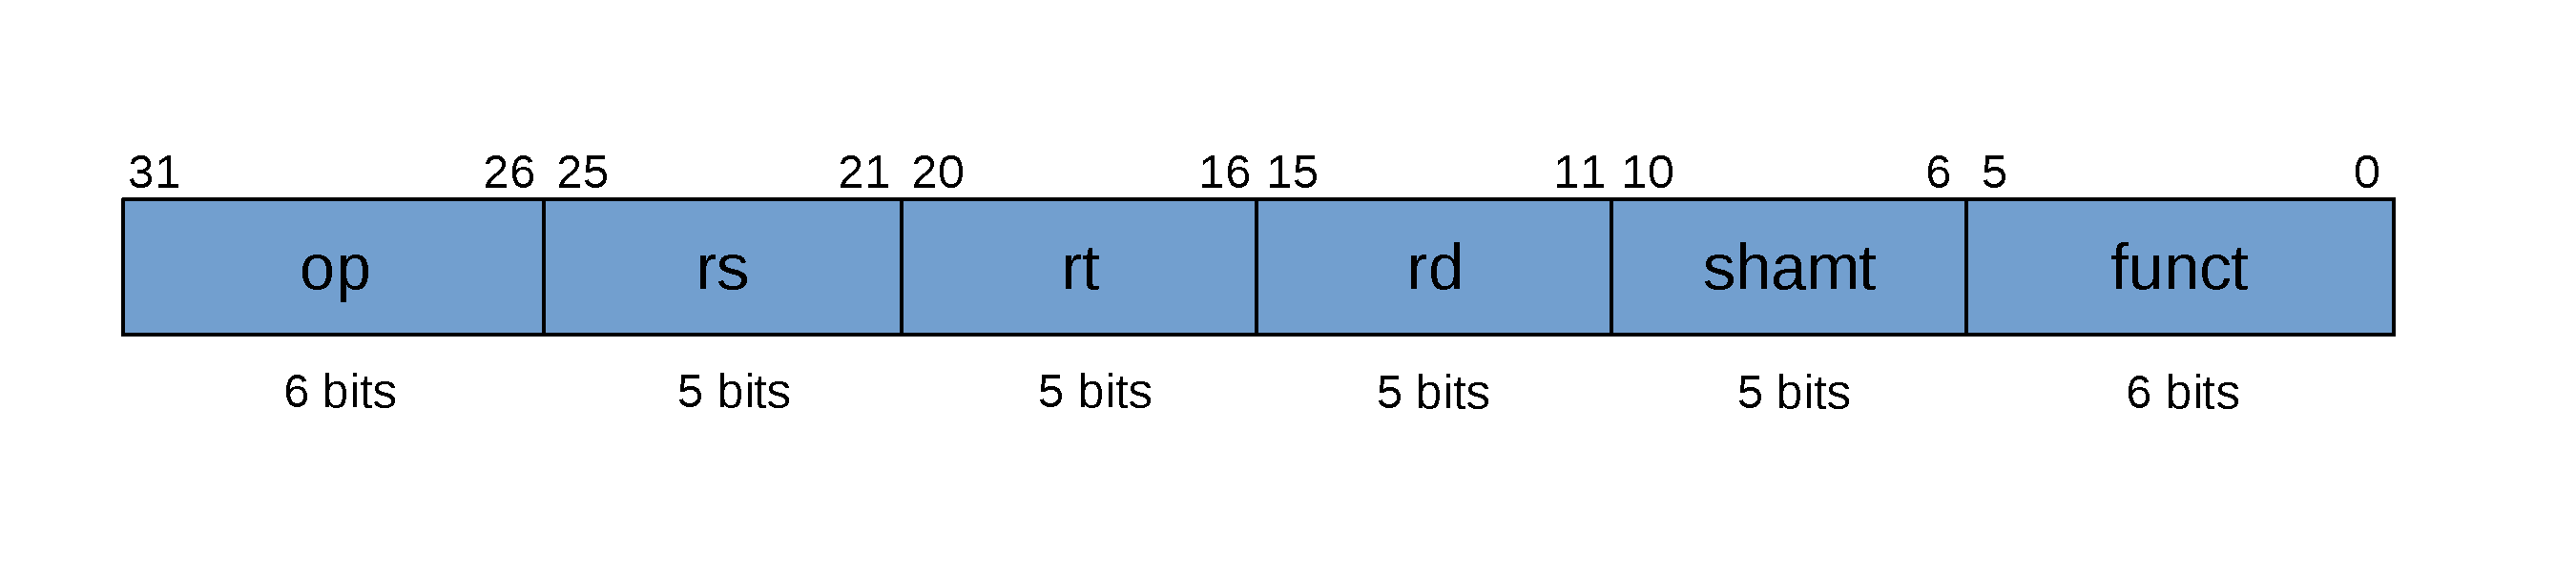
\includegraphics[width=10cm]{rtype.pdf}
\end{center}

\scriptsize

\vspace{-0.3cm}

\begin{itemize}
\item \textcolor{red}{op}: Opcode of the instruction, \texttt{op} $=$ \texttt{000000} for all R-type instructions.
\vspace{0.1cm}
\item \textcolor{red}{rs}: First source operand.
\vspace{0.1cm}
\item \textcolor{red}{rt}: Second source operand.
\vspace{0.1cm}
\item \textcolor{red}{rd}: Destination.
\vspace{0.1cm}
\item \textcolor{red}{shamt}: Shift amount. It is only used in shift operations (so it is \texttt{00000} for us).
\vspace{0.1cm}
\item \textcolor{red}{funct}: Specify the function to use.
  \begin{itemize}
    \scriptsize
  \item \lstinline{add} has \texttt{funct = 100000}.
  \item \lstinline{sub} has \texttt{funct = 100010}.
  \item \lstinline{and} has \texttt{funct = 100100}.
  \item \lstinline{or}\texttt{ }  has \texttt{funct = 100101}.
  \item \lstinline{slt} has \texttt{funct = 101010}.
  \end{itemize}

\end{itemize}

\end{frame}

\begin{frame}[fragile]
\frametitle{R-Type Example}

\scriptsize

\begin{lstlisting}
  add $t1, $t0, $0  # $t1 @\textcolor{darkgreen}{$\leftarrow$}@ $t0 + 0
  sub $t2, $t3, $t1 # $t2 @\textcolor{darkgreen}{$\leftarrow$}@ $t3 - $t1
  slt $t4, $t4, $t2 # $t4 @\textcolor{darkgreen}{$\leftarrow$}@ 1 if $t4 < $t2 else 0
\end{lstlisting}

\vspace{0.5cm}

The machine language representation of this code is\\
\vspace{0.2cm}

\begin{center}
\begin{tabular}{|l|c|c|c|c|c|c|}
  \hline
  \multicolumn{1}{|c|}{Instruction} & op & rs & rt & rd & shamt & funct\\
  \hline
  \hline
  \lstinline!add $t1, $t0, $0! & 000000 & 01000 & 00000 & 01001 & 00000 & 100000\\
  \hline
  \lstinline!sub $t2, $t3, $t1! & 000000 & 01011 & 01001 & 01010 & 00000 & 100010\\
  \hline
  \lstinline!slt $t4, $t4, $t2! & 000000 & 01100 & 01010 & 01100 & 00000 & 101010\\
  \hline
\end{tabular}
\end{center}

\end{frame}

\subsection{I-Type Instructions}

\begin{frame}%[fragile]
\frametitle{I(mmediate)-Type Instructions}

\begin{center}
  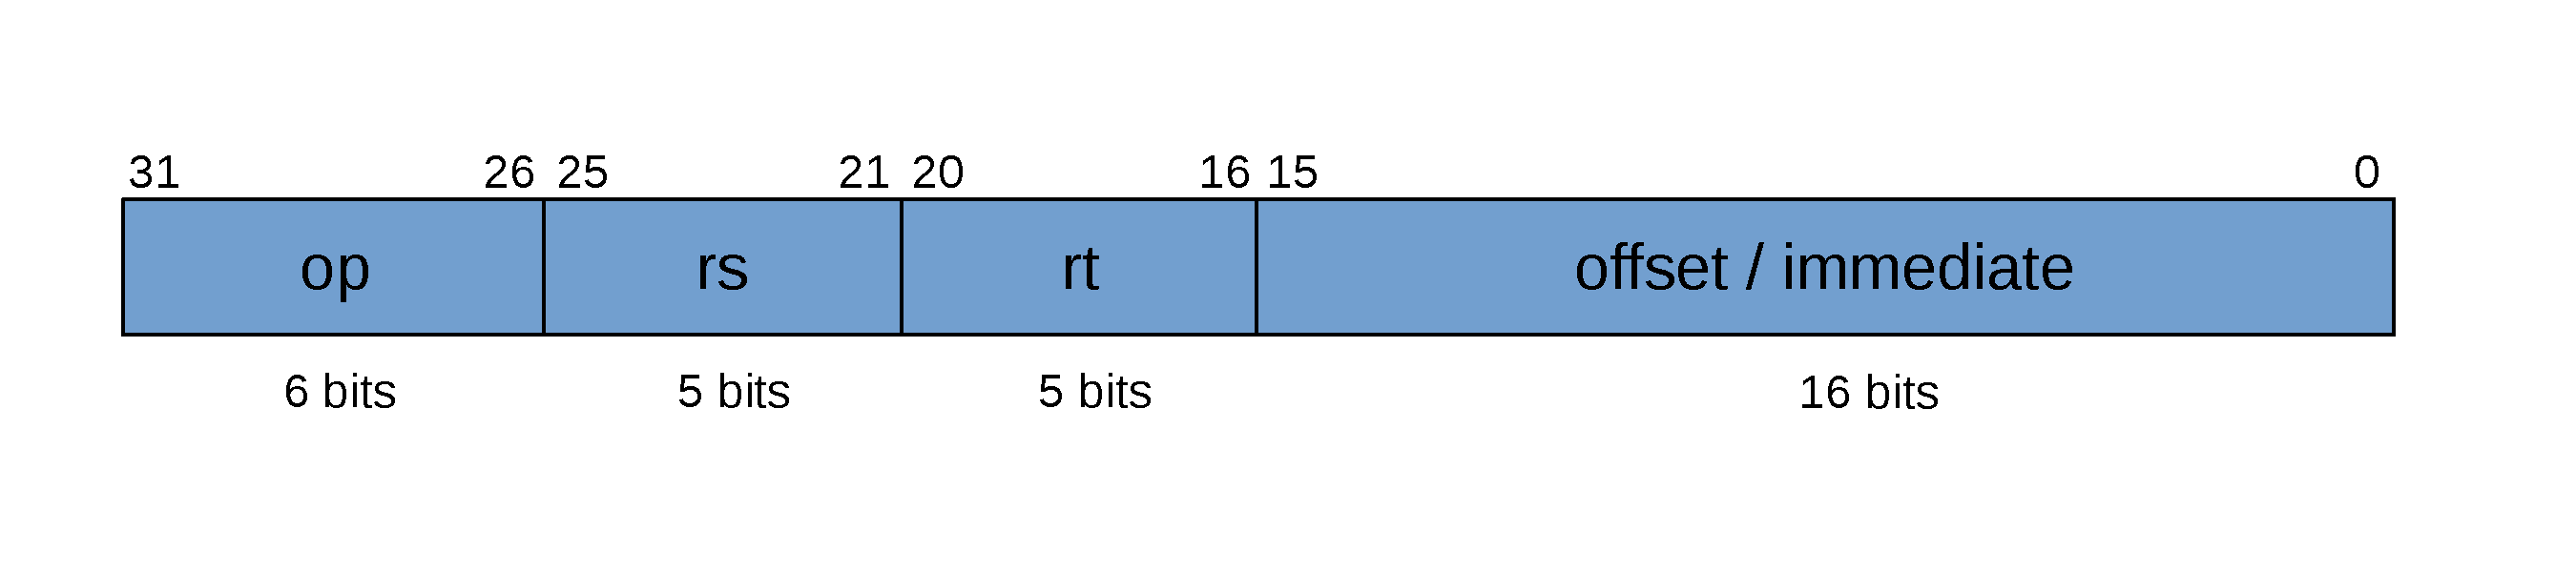
\includegraphics[width=10cm]{itype.pdf}
\end{center}

\vspace{-0.3cm}

\scriptsize

\begin{itemize}
\item \textcolor{red}{op}: Opcode of the instruction,
  \begin{itemize}
    \scriptsize
  \item \lstinline{lw}\texttt{  } has \texttt{op = 100011}.
  \item \lstinline{sw}\texttt{  } has \texttt{op = 101011}.
  \item \lstinline{addi} has \texttt{op = 001000}.
  \item \lstinline{beq}\texttt{ }  has \texttt{op = 000100}.
  \end{itemize}
\vspace{0.1cm}
\item \textcolor{red}{rs}: Register containing the base address for \lstinline{lw} and \lstinline{sw}, and a source operand for
  \lstinline{addi} and \lstinline{beq}.
\vspace{0.1cm}
\item \textcolor{red}{rt}: Destination register for \lstinline{addi} and \lstinline{lw}, source register for \lstinline{sw} and second
  operand for \lstinline{beq}.
\vspace{0.1cm}
\item \textcolor{red}{offset/immediate}: Byte address offset for \lstinline{lw} and \lstinline{sw}, immediate field for \lstinline{addi} and
  word address offset with respect to \textcolor{red}{\texttt{PC} $+\ 4$} for \lstinline{beq}. This value is sign extended to a $32$-bit value.

\end{itemize}

\end{frame}

\begin{frame}[fragile]
\frametitle{I-Type Example}

\scriptsize

\begin{lstlisting}
  lw   $t1, 32($s0)   # $t1 @\textcolor{darkgreen}{$\leftarrow$}@ Memory[$s0 + 32]
  addi $t1, $t1, 1975 # $t1 @\textcolor{darkgreen}{$\leftarrow$}@ $t1 + 1975
  beq  $t2, $t1, end  # if $t2 = $t1 goto end
  addi $t1, $t1, 1    # $t1 @\textcolor{darkgreen}{$\leftarrow$}@ $t1 + 1
end:
  sw   $t1, 32($s0)   # Memory[$s0 + 32] @\textcolor{darkgreen}{$\leftarrow$}@ $t1
\end{lstlisting}

\vspace{0.5cm}

The machine language representation of this code is\\
\vspace{0.2cm}

\begin{center}
\begin{tabular}{|l|c|c|c|c|}
  \hline
  \multicolumn{1}{|c|}{Instruction} & op & rs & rt & offset/immediate\\
  \hline
  \hline
  \lstinline!lw $t1, 32($s0)! & 100011 & 10000 & 01001 & 0000000000100000 \\
  \hline
  \lstinline!addi $t1, $t1, 1975! & 001000 & 01001 & 01001 & 0000011110110111\\
  \hline
  \lstinline!beq $t2, $t1, end! & 000100 & 01010 & 01001 & 0000000000000001\\
  \hline
  \lstinline!addi $t1, $t1, 1! & 001000 & 01001 & 01001 & 0000000000000001\\
  \hline
  \lstinline!sw $t1, 32($s0)! & 101011 & 10000 & 01001 & 0000000000100000\\
  \hline
\end{tabular}
\end{center}

\end{frame}

\subsection{J-Type Instructions}


\begin{frame}%[fragile]
\frametitle{J(ump)-Type Instructions}

\begin{center}
  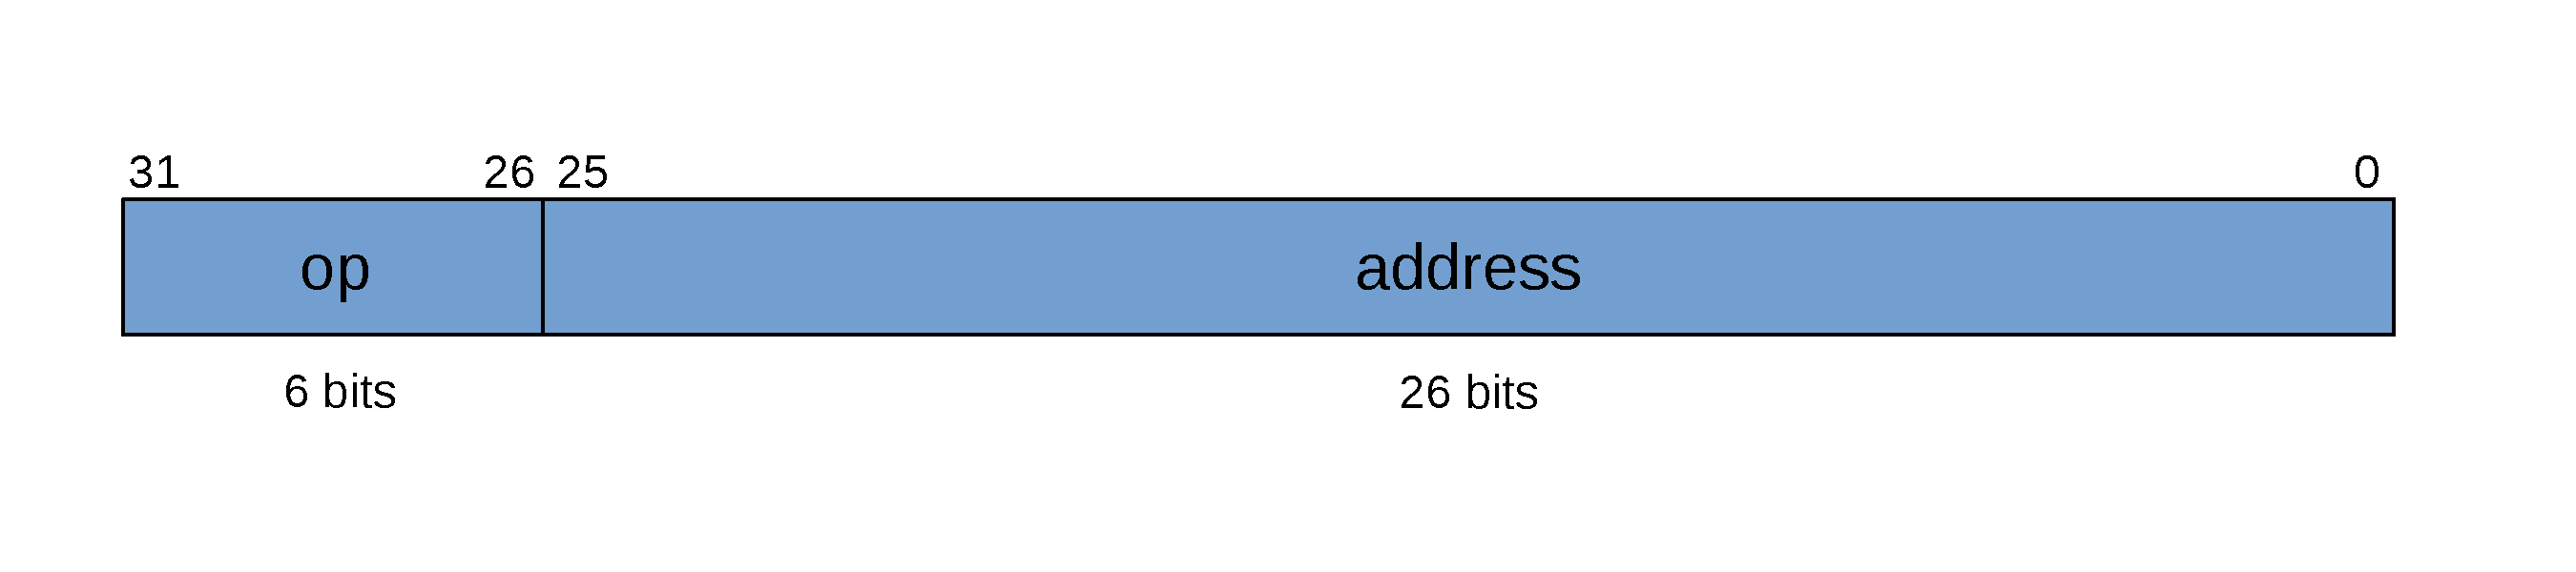
\includegraphics[width=10cm]{jtype.pdf}
\end{center}

\vspace{-0.3cm}

\begin{itemize}
\item \textcolor{red}{op}: Opcode of the instruction, \texttt{op = 000010}
\vspace{0.2cm}
\item \textcolor{red}{address}: word address of the instruction to jump to. To get a $32$-bit jump address,
  \begin{itemize}
  \item \textcolor{red}{address} is multiplied by $4$.
  \item The four high order bits are taken from the four high order bits of PC $+\ 4$.
  \end{itemize}
\item The jump is limited to the region \textcolor{blue}{$[$PC + 4$]_{31..28}[$\texttt{0x0000000}$]$} to \textcolor{blue}{$[$PC + 4$]_{31..28}[$\texttt{0xffffffc}$]$}.
\end{itemize}

\end{frame}

\begin{frame}[fragile]
\frametitle{J-Type Example}

\scriptsize

\begin{lstlisting}
0x00400000: beq $s3, $s4, else # if $s3 == $s4 goto else
0x00400004: add $s0, $s1, $s2  # $s0 @\textcolor{darkgreen}{$\leftarrow$}@ $s1 + $s2
0x00400008: j endif            # goto endif
else:
0x0040000d: sub $s0, $s1, $s2  # $s0 @\textcolor{darkgreen}{$\leftarrow$}@ $s1 - $s2
endif:
0x00400010:
\end{lstlisting}

\vspace{0.5cm}

The machine language representation of line $3$ is\\
\vspace{0.2cm}

\begin{center}
\begin{tabular}{|l|c|c|c|c|}
  \hline
  \multicolumn{1}{|c|}{Instruction} & op & address\\
  \hline
  \hline
  \lstinline!j endif! & 000010 & 00000100000000000000000100\\
  \hline
\end{tabular}
\end{center}

\end{frame}

\subsection{Program Example}

\begin{frame}[fragile]
\frametitle{Program Example}

To write a more interesting program, we add three more MIPS instructions (we don't use them in our simplified
version of MIPS):\\

\vspace{0.4cm}

\begin{itemize}
\item \lstinline{jal fct}: Call the function \lstinline{fct} and save in register \lstinline{$ra} the address of the next instruction (the one just
  after the \lstinline{jal} instruction).
 \vspace{0.2cm}

\item \lstinline{jr reg}: Jump to the address contained in register \lstinline{reg}.
  \vspace{0.2cm}

\item \lstinline{mul dst, src1, src2}: Multiplies register \lstinline{src1} with register \lstinline{src2} and puts the result in register \lstinline{reg}.
\end{itemize}

\end{frame}

\begin{frame}%[fragile]
\frametitle{Calling Convention (Simplified)}

\scriptsize

\begin{itemize}

\item The first four arguments are passed in registers: \textcolor{blue}{\lstinline!$a0!},
  \textcolor{blue}{\lstinline!$a1!}, \textcolor{blue}{\lstinline!$a2!} and \textcolor{blue}{\lstinline!$a3!}.

\vspace{0.2cm}

\item Additional arguments are passed on the stack before calling the function:
  \begin{itemize}
    \scriptsize
  \item $\texttt{arg}_n$ is pushed.
  \item Then, $\texttt{arg}_{n-1}$ is pushed.
  \item \ldots
  \item Then, $\texttt{arg}_5$ is pushed.
  \end{itemize}

\vspace{0.2cm}

\item The stack pointer (\textcolor{blue}{\lstinline!$sp!}) must be $4$-byte aligned before calling a function.

\vspace{0.2cm}

\item To reduce the effort to save and restore registers, we define two types of registers. A function
  must save and restore any of the preserved registers it uses. But it can change the nonpreserved registers freely.

  \begin{center}
  \begin{tabular}{|l|l|}
    \hline
    \multicolumn{1}{|c|}{Preserved} & \multicolumn{1}{|c|}{Nonpreserved}\\
    \hline
    \hline
    Saved registers: \textcolor{blue}{\lstinline!$s0-$s7!} & Temporary registers: \textcolor{blue}{\lstinline!$t0-$t9!}\\
    \hline
    Return address: \textcolor{blue}{\lstinline!$ra!} & Argument registers: \textcolor{blue}{\lstinline!$a0-$a3!}\\
    \hline
    Stack pointer: \textcolor{blue}{\lstinline!$sp!} & Return value registers: \textcolor{blue}{\lstinline!$v0-$v1!}\\
    \hline
    Stack \textcolor{blue}{above} the stack pointer & Stack \textcolor{blue}{below} the stack pointer\\
    \hline
  \end{tabular}
\end{center}

\end{itemize}

\end{frame}

\begin{frame}[fragile]
\frametitle{Recursive Factorial}

\scriptsize

\begin{lstlisting}
factorial:
# from Digital Design and Computer Architecture
        addi $sp, $sp, -8  # make room on stack for two 4 bytes values
        sw   $a0, 4($sp)   # store $a0
        sw   $ra, 0($sp)   # store $ra
        addi $t0, $0, 2    # $t0 @\textcolor{darkgreen}{$\leftarrow$}@ 2
        slt  $t0, $a0, $t0 # n @\textcolor{darkgreen}{$\le$}@ 1 ?
        beq  $t0, $0, else # no: goto else
        addi $v0, $0, 1
        addi $sp, $sp, 8   # restore $sp
        jr   $ra           # return 1
else:
        addi $a0, $a0, -1  # n @\textcolor{darkgreen}{$\leftarrow$}@ n - 1
        jal  factorial     # recursive call
        lw   $ra, 0($sp)   # restore $ra
        lw   $a0, 4($sp)   # restore $a0
        addi $sp, $sp, 8   # restore $sp
        mul  $v0, $a0, $v0
        jr   $ra           # return n * factorial(n - 1)
\end{lstlisting}


\end{frame}

\begin{frame}[fragile]
\frametitle{Recursive Factorial}

\scriptsize

\begin{lstlisting}
main:
        addi $a0, $0, 5
        jal  factorial     # factorial(5)
        add  $a0, $v0, $0
        addi $v0, $0, 1    # 1 is syscall number for print_int
        syscall            # print_int
        addi $v0, $0, 10   # 10 is syscall number for exit
        syscall            # exit

# spim -file factorial.s
# output: 120
\end{lstlisting}

\end{frame}

\lstset{language=C}

\begin{frame}[fragile]
\frametitle{\exo}

Translate the following \texttt{C} function in MIPS assembly.

\vspace{1cm}

\begin{lstlisting}
int fibonacci(int n)
{
  if (n < 2) return n;
  return fibonacci(n - 1) + fibonacci(n - 2);
}
\end{lstlisting}

\end{frame}

\lstset{language=[mips]Assembler}

\ifanswers
\begin{frame}[fragile]
\frametitle{Solution}
\scriptsize
\begin{lstlisting}
fibonacci:
        addi $t0, $0, 2    # $t0 = 2
        slt  $t0, $a0, $t0 # n @\textcolor{darkgreen}{$\le$}@ 1 ?
        beq  $t0, $0, else # no: goto else
        add  $v0, $a0, $0  # $v0 @\textcolor{darkgreen}{$\leftarrow$}@ n
        jr   $ra           # return n
else:
        addi $sp, $sp, -12 # make room on stack
        sw   $a0, 8($sp)   # store $a0
        sw   $ra, 4($sp)   # store $ra
        sw   $s0, 0($sp)   # store $s0
        addi $a0, $a0, -1  # n @\textcolor{darkgreen}{$\leftarrow$}@ n - 1
        jal  fibonacci
        add  $s0, $v0, $0  # $s0 @\textcolor{darkgreen}{$\leftarrow$}@ fibonacci(n - 1)
        addi $a0, $a0, -1  # n @\textcolor{darkgreen}{$\leftarrow$}@ n - 2
        jal  fibonacci
        add  $v0, $s0, $v0 # $v0 @\textcolor{darkgreen}{$\leftarrow$}@ fibonacci(n - 1) + fibonacci(n - 2)
\end{lstlisting}

\end{frame}

\begin{frame}[fragile]
\frametitle{Solution}
\scriptsize
\begin{lstlisting}
        lw   $s0, 0($sp)   # restore $s0
        lw   $ra, 4($sp)   # restore $ra
        lw   $a0, 8($sp)   # restore $a0
        addi $sp, $sp, 12  # restore $sp
        jr   $ra           # return

main:
        addi $a0, $0, 16
        jal  fibonacci     # fibonacci(16)
        add  $a0, $v0, $0
        addi $v0, $0, 1
        syscall            # print_int
        addi $v0, $0, 10
        syscall            # exit

# spim -file fibonacci.s
# output: 987
\end{lstlisting}

\end{frame}

\fi

\section{Single-Cycle Datapath}

\subsection{Overview}

\begin{frame}%[fragile]
\frametitle{Overview}

\begin{itemize}

\item We build a datapath for our simple \texttt{MIPS} processor.

\vspace{0.5cm}

\item Each instruction is executed in one clock cycle.

\vspace{0.5cm}

\item We use two separate memories, one for the instructions and one for the data.

\end{itemize}

\end{frame}

\begin{frame}[fragile]
\frametitle{Program Example}

We use the following program to demonstrate the datapath.

\vspace{0.5cm}

\scriptsize
\begin{lstlisting}
main:
        add  $t0, $0, $0
        addi $t1, $0, 1
        lw   $t2, 0($0)
        addi $t2, $t2, 1
loop:
        slt  $t3, $t1, $t2
        beq  $t3, $0, endloop
        add  $t0, $t0, $t1
        addi $t1, $t1, 1
        b loop
endloop:
        sw $t0, 4($0)
        b endloop
\end{lstlisting}

\end{frame}

\begin{frame}%[fragile]
\frametitle{\exo}

What does this program do?

\end{frame}

\subsection{Datapath Elements}

\begin{frame}%[fragile]
\frametitle{Elements Used to Build the Datapath}

\begin{itemize}

\item \textcolor{blue}{Instruction memory}.
  \begin{itemize}
  \item It contains the program.
  \item The output is the $4$ bytes starting at the specified address.
  \end{itemize}
  \vspace{0.2cm}

\item \textcolor{blue}{Data memory}.
  \begin{itemize}
  \item It contains the data.
  \item The output is the $4$ bytes starting at the specified address, when the \texttt{RD} pin is active.
  \item You write a $4$ bytes word in the memory, at the rising edge of the clock, by specifying the address and activating the
    \texttt{WR} pin.
  \end{itemize}
  \vspace{0.2cm}

\item \textcolor{blue}{Register file}.
  \begin{itemize}
  \item It contains the $32$ four bytes registers.
  \item You can read two registers at a time, by specifying their five bits number.
  \item You can write to a register, at the rising edge, by specifying a register number and the data to write to it.
  \end{itemize}

\end{itemize}

\end{frame}

\begin{frame}%[fragile]
\frametitle{Elements Used to Build the Datapath}

\begin{itemize}

\item \textcolor{blue}{Arithmetic and logic unit}.
  \begin{itemize}
  \item It performs the different arithmetic and logic computations (addition, substraction, and, or, nor, set and less than).
  \item It gives information about the result of the computation (negative, zero, overflow, carry bit).
  \end{itemize}

\vspace{0.5cm}

\item \textcolor{blue}{Program counter}.
  \begin{itemize}
  \item A register that contains the next instruction to fetch.
  \end{itemize}

\end{itemize}

\end{frame}

\begin{frame}%[fragile]
\frametitle{Abstract View of the Implementation}

\begin{center}
\hspace*{-1cm}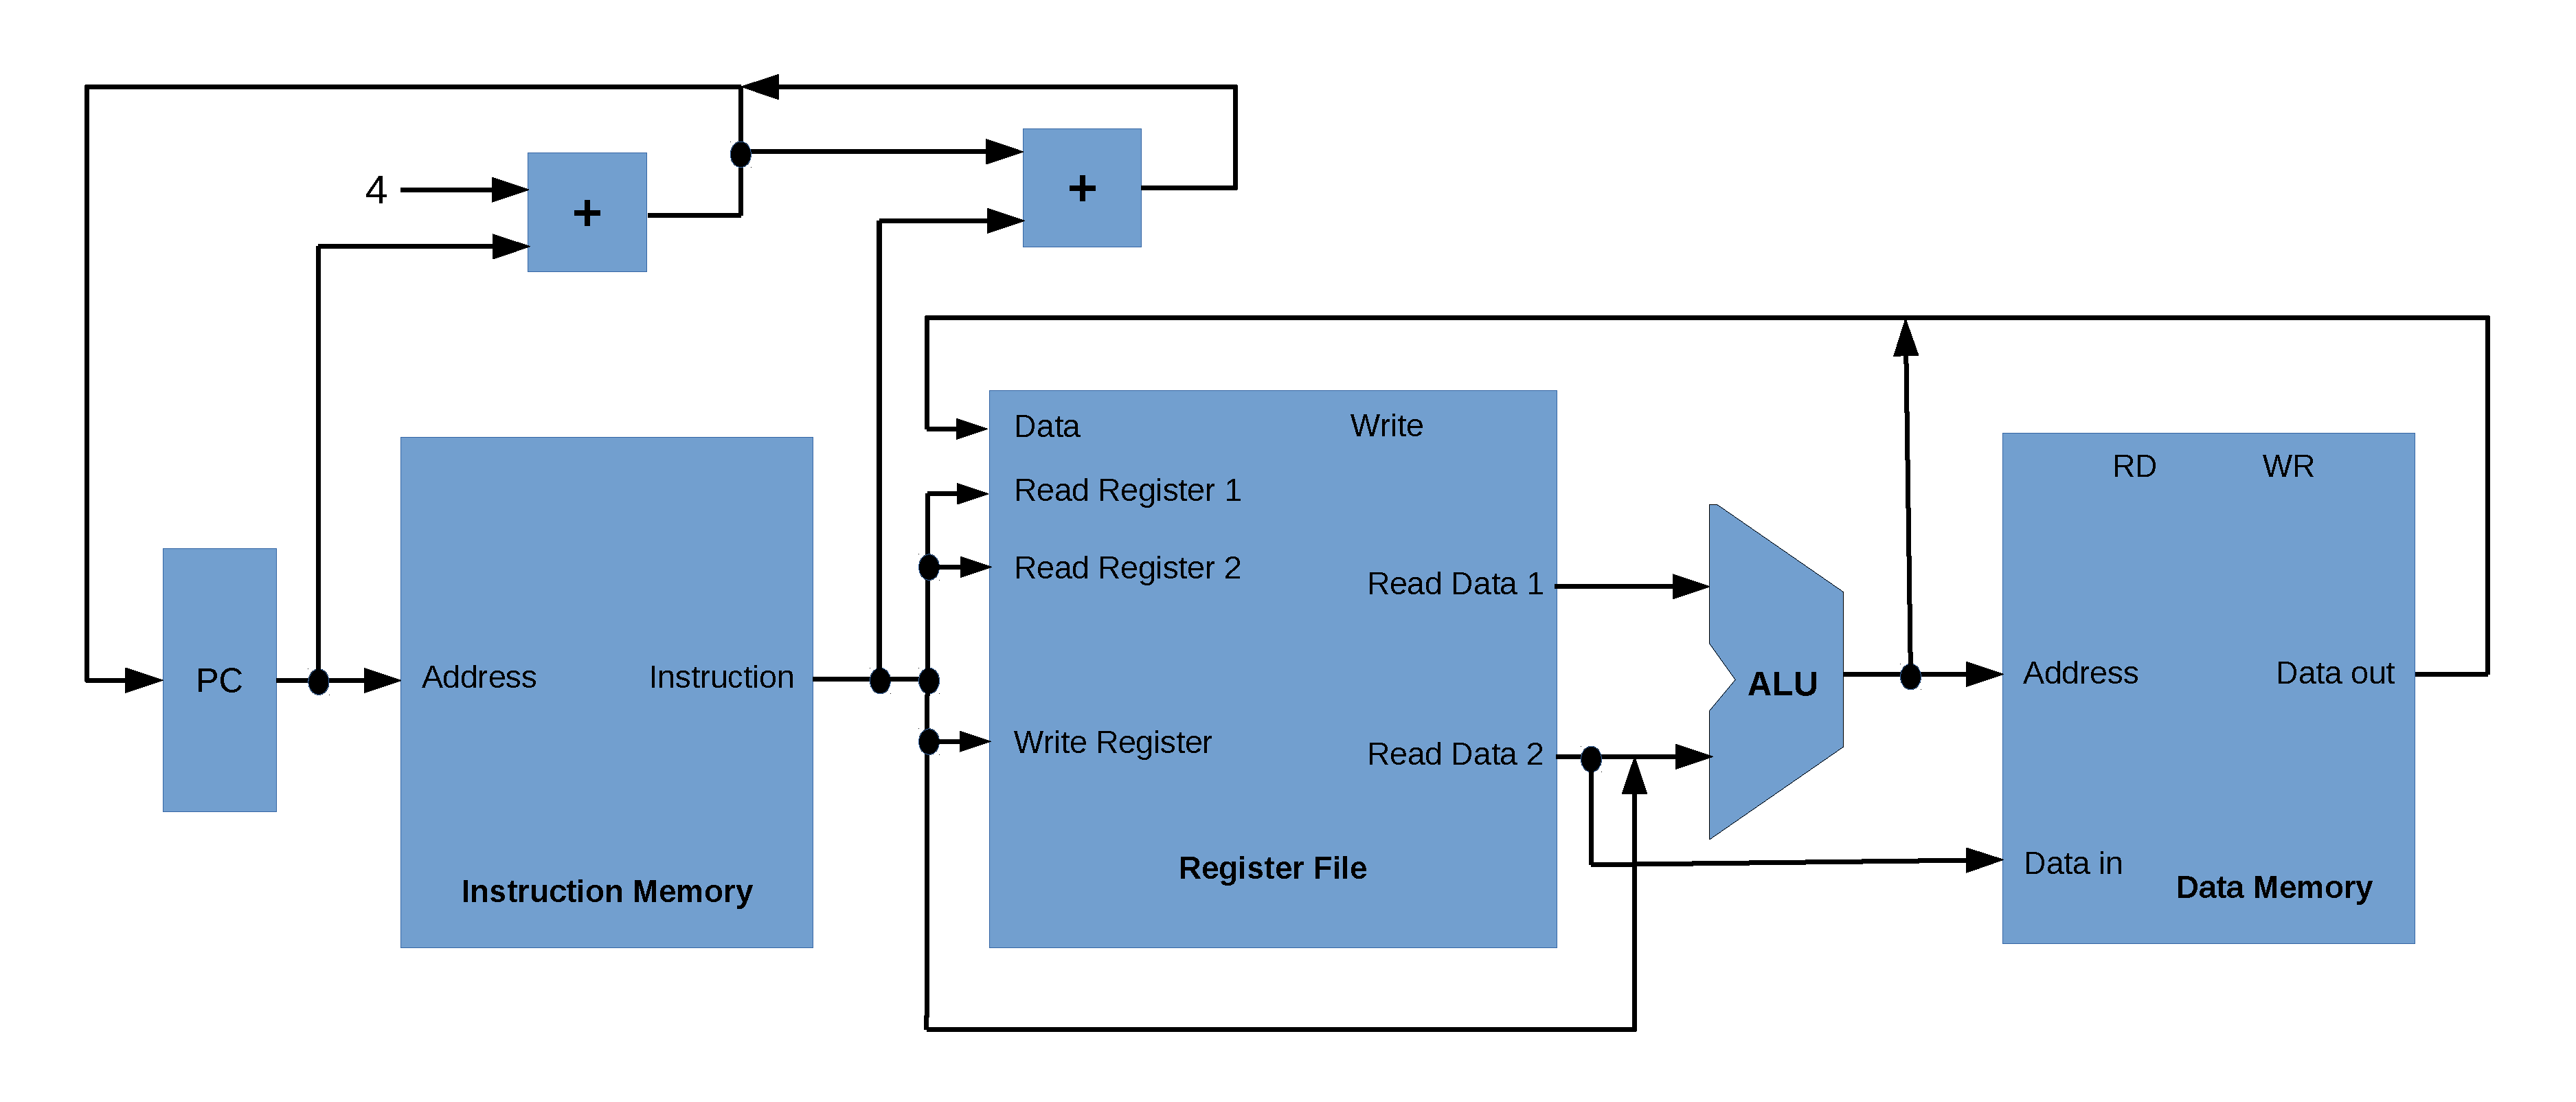
\includegraphics[width=12.5cm]{abstract_view.pdf}
\end{center}

\end{frame}

%% \begin{frame}%[fragile]
%% \frametitle{Instruction Memory and Program Counter}

%% \end{frame}

%% \begin{frame}%[fragile]
%% \frametitle{Data Memory}

%% \end{frame}

%% \begin{frame}%[fragile]
%% \frametitle{Program Counter}

%% \end{frame}

%% \begin{frame}%[fragile]
%% \frametitle{Register File}

%% \end{frame}

%% \begin{frame}%[fragile]
%% \frametitle{Arithmetic and Logic Unit}

%% \end{frame}

%% \begin{frame}%[fragile]
%% \frametitle{Adder, Shift, Sign-extend}

%% \end{frame}

\subsection{Datapath Implementation}

\begin{frame}%[fragile]
\frametitle{Instruction Memory and Fetching}

\end{frame}

\begin{frame}%[fragile]
\frametitle{J-Type Instruction}

\end{frame}

\begin{frame}%[fragile]
\frametitle{R-Type Instruction}

\end{frame}

\begin{frame}%[fragile]
\frametitle{I-Type Instruction}

\end{frame}

\begin{frame}%[fragile]
\frametitle{Complete Datapath}

\begin{center}
\hspace*{-1cm}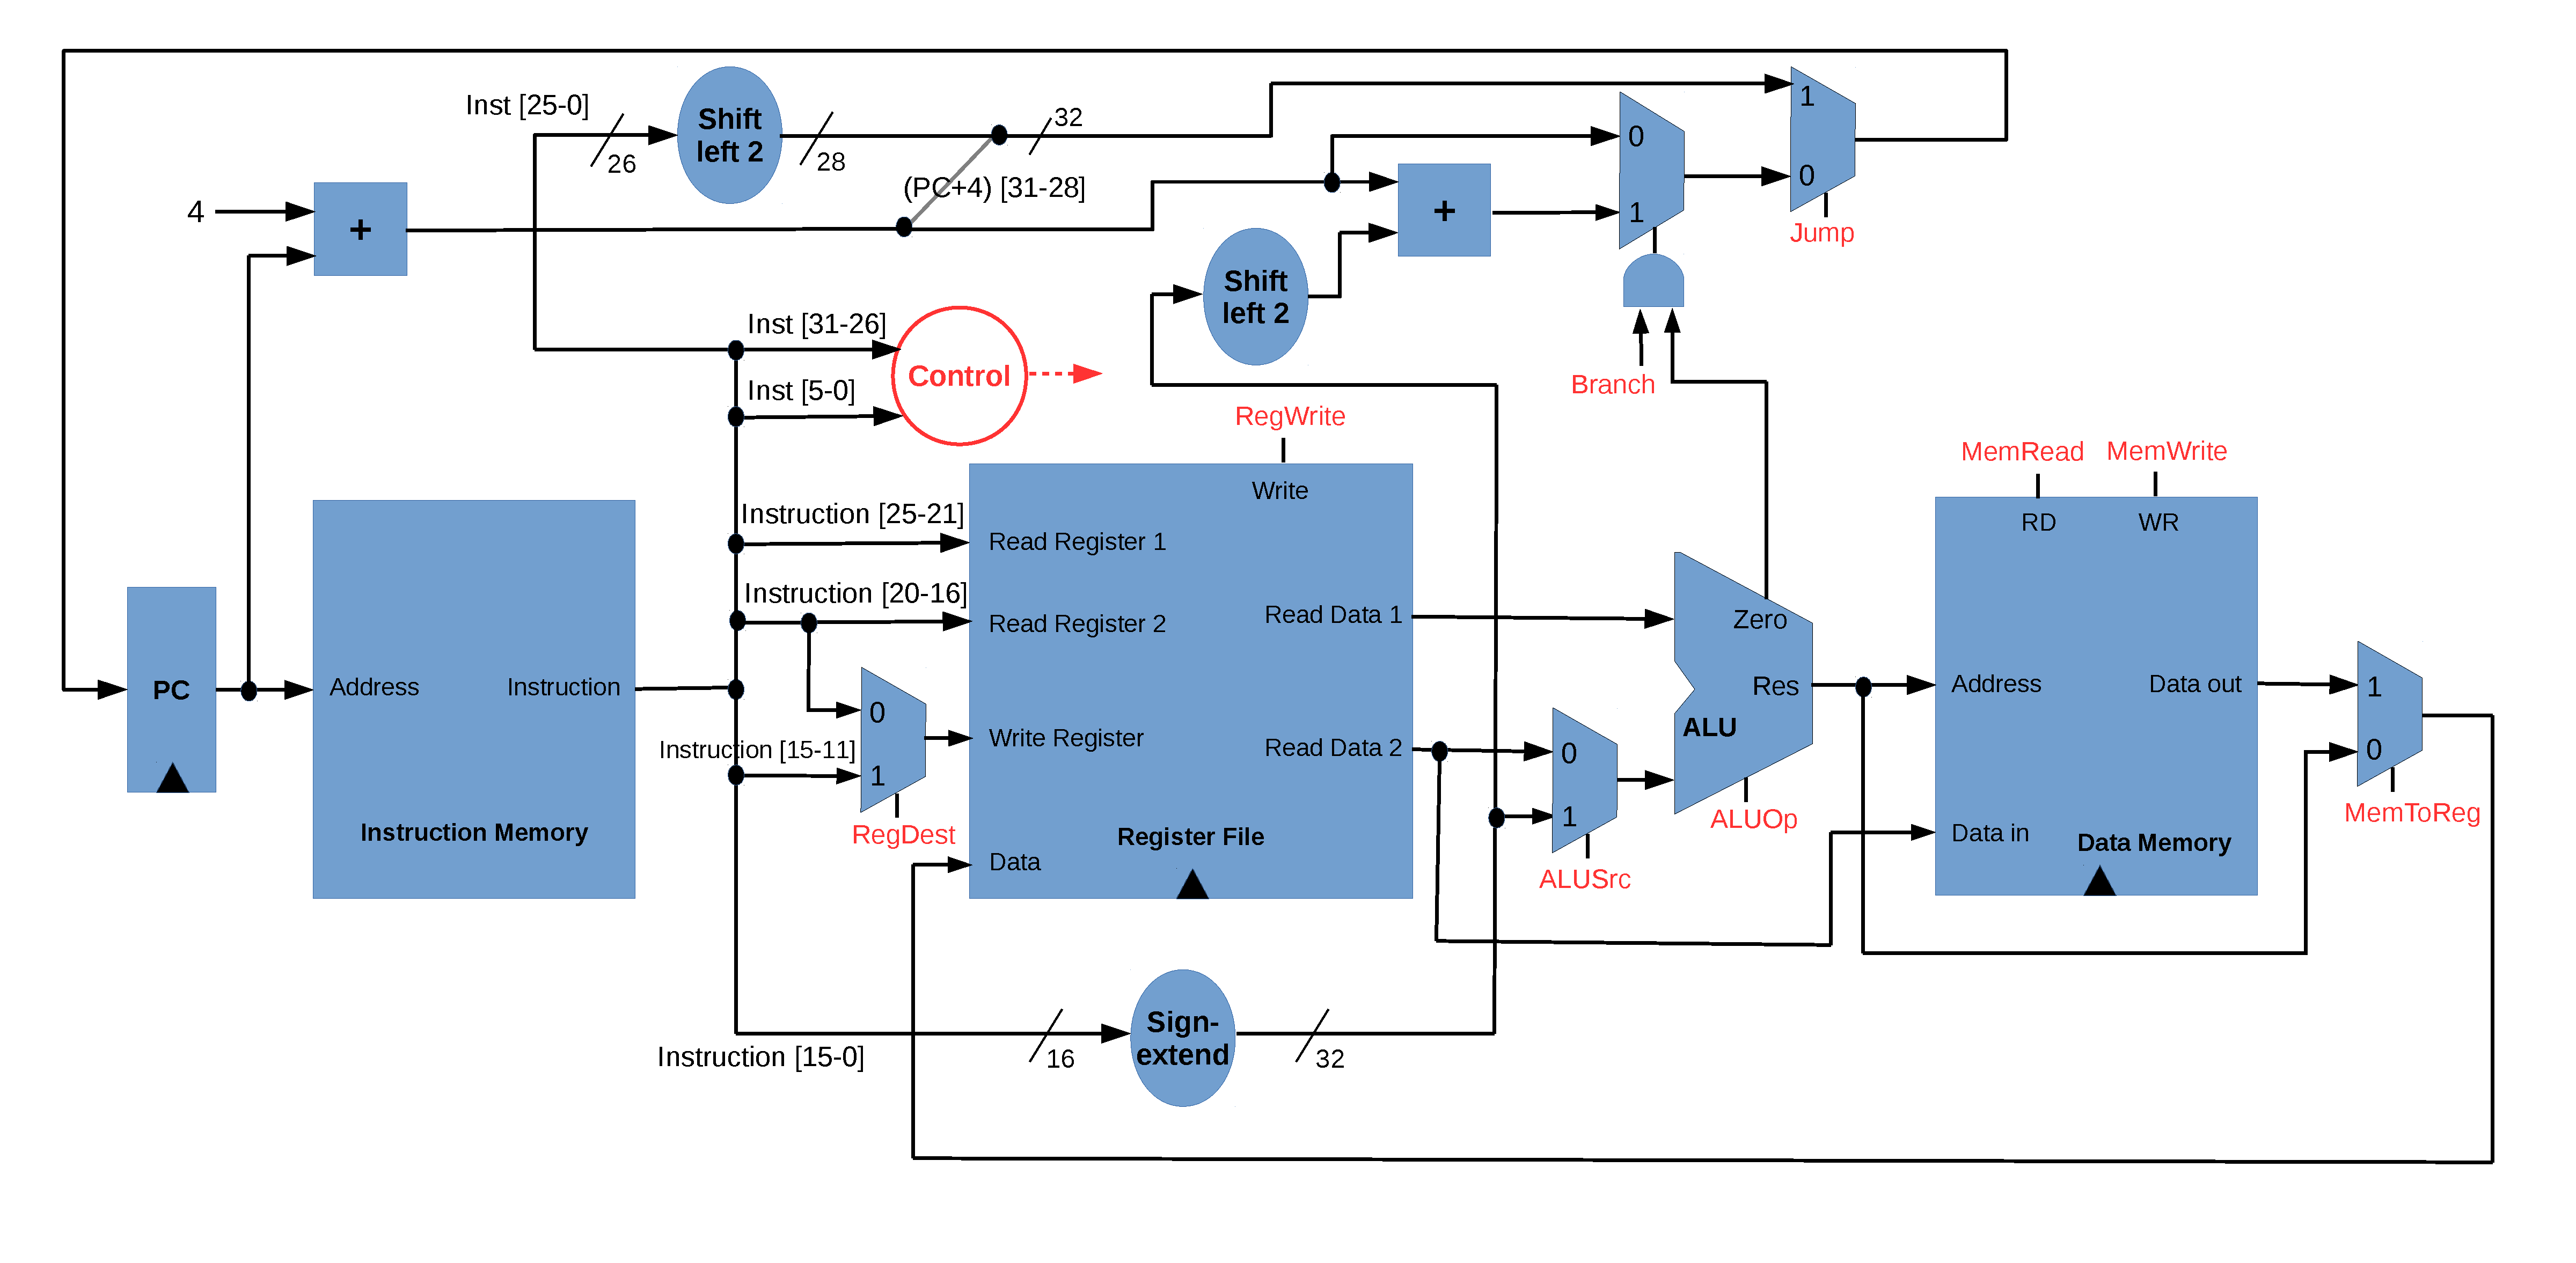
\includegraphics[width=13cm]{complete_single_cycle.pdf}
\end{center}

\end{frame}

\subsection{Running a Program}

\begin{frame}%[fragile]
\frametitle{Running a Program}

\end{frame}


\subsection{Inefficiency}

\begin{frame}%[fragile]
\frametitle{Inefficiency}

\end{frame}

\section{Multi-Cycle Datapath}

\subsection{Overview}

\begin{frame}%[fragile]
\frametitle{Overview}

\begin{itemize}

\item The single-cycle datapath executes each instructions in one clock cycle regardless
  of the complexity of the instructions.

  \vspace{0.2cm}

\item The key design point of the multi-cycle datapath is to divide the execution of an instruction
  into several small steps.

  \vspace{0.2cm}

\item Then we can use more cycles to execute complex instructions and use fewer cycles to execute simple
  instructions.

  \vspace{0.2cm}

\item An instruction is divided at most into the following five stages (an instruction can take less
  than five stages):
  \begin{itemize}
  \item Instruction fetch (\textcolor{blue}{IF}).
  \item Instruction decode and operand fetch (\textcolor{blue}{ID}).
  \item Execution (\textcolor{blue}{EXE}).
  \item Memory access (\textcolor{blue}{MEM}).
  \item Write back (\textcolor{blue}{WB}).
  \end{itemize}

\end{itemize}

\end{frame}

\begin{frame}%[fragile]
\frametitle{Abstract View of the Implementation}

\begin{center}
\hspace*{-0.75cm}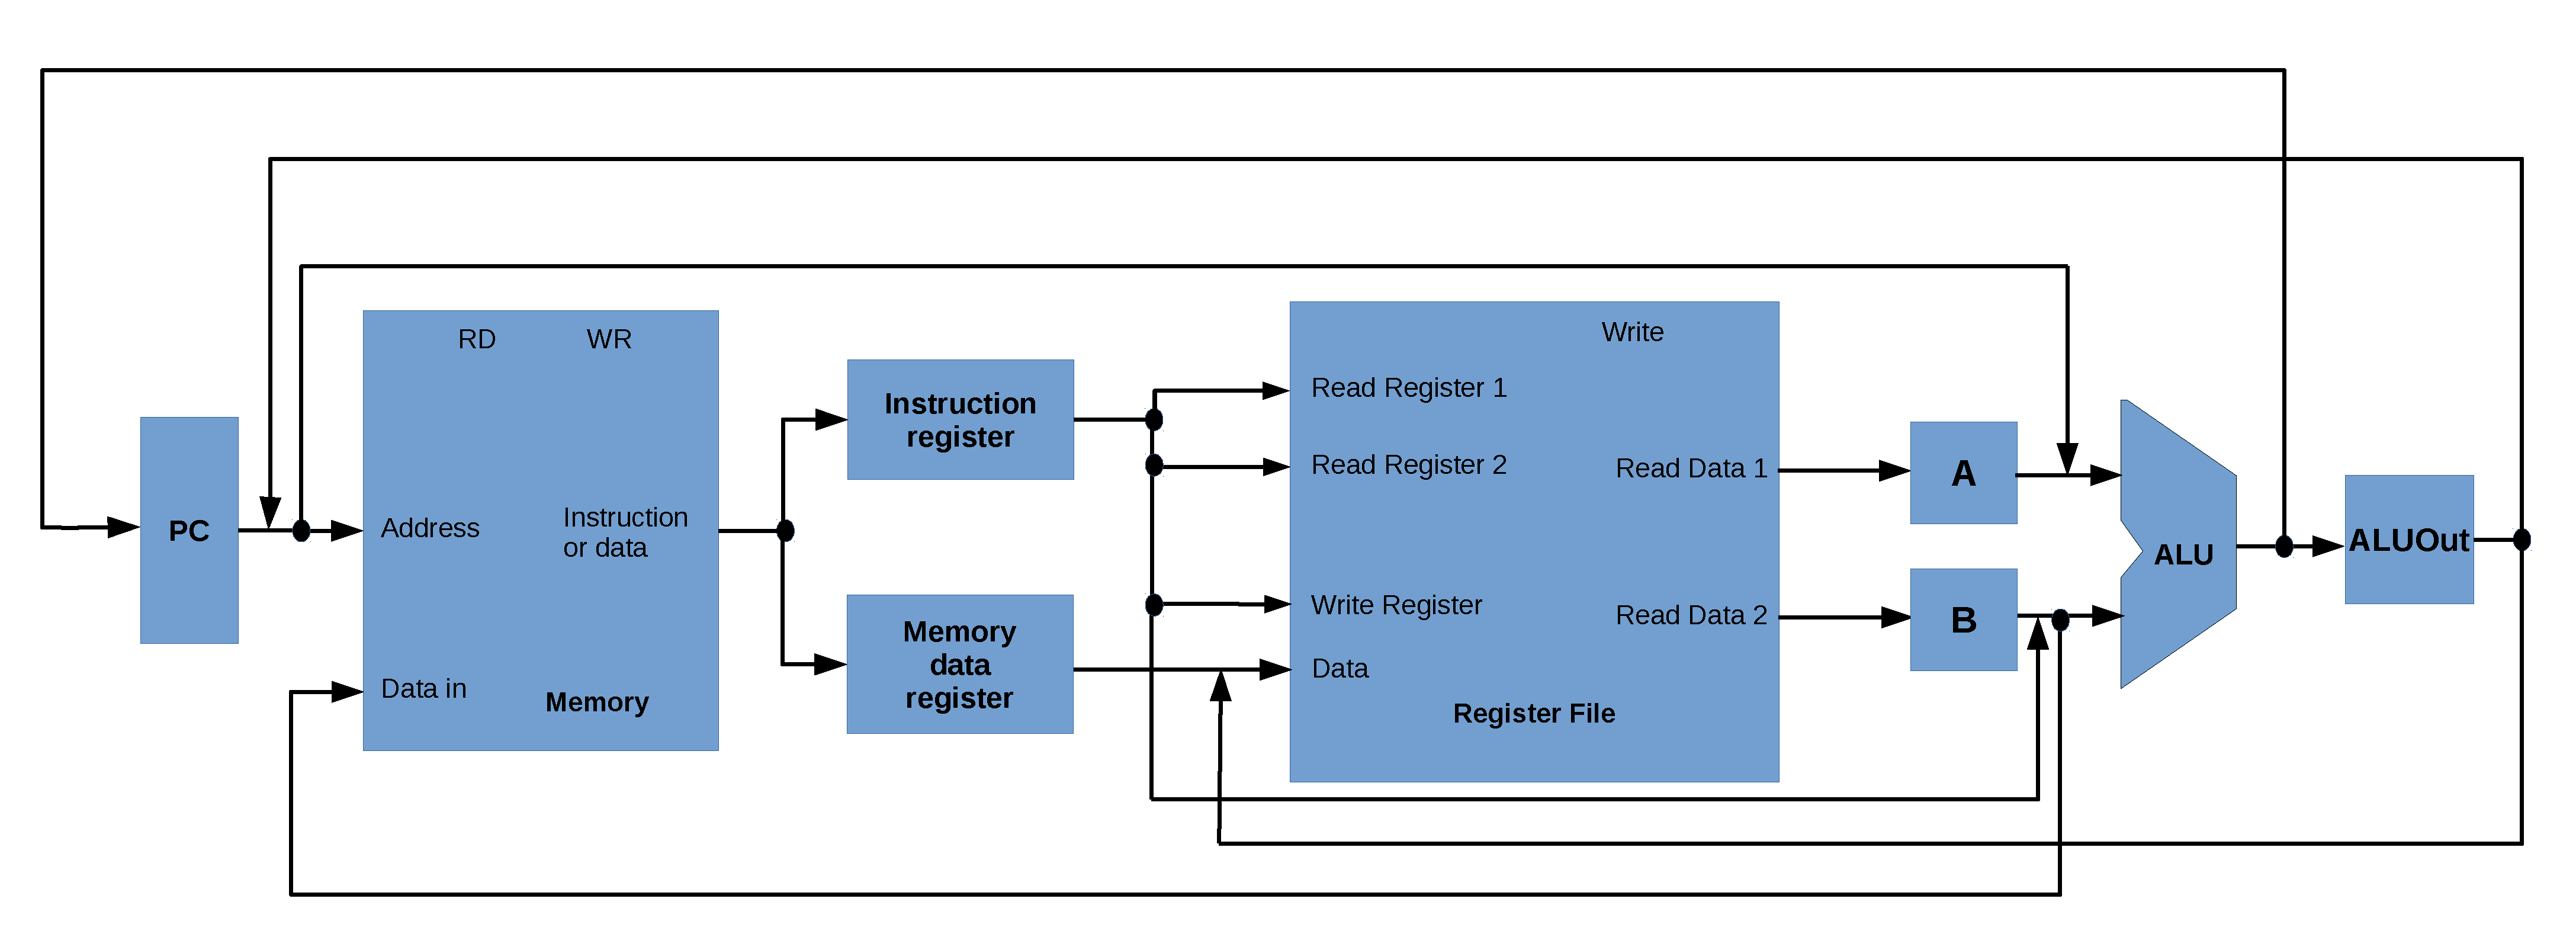
\includegraphics[width=12.5cm]{abstract_view_multi.pdf}
\end{center}

\end{frame}

\subsection{Datapath Implementation}

\begin{frame}%[fragile]
\frametitle{Complete Datapath}

\begin{center}
\hspace*{-1cm}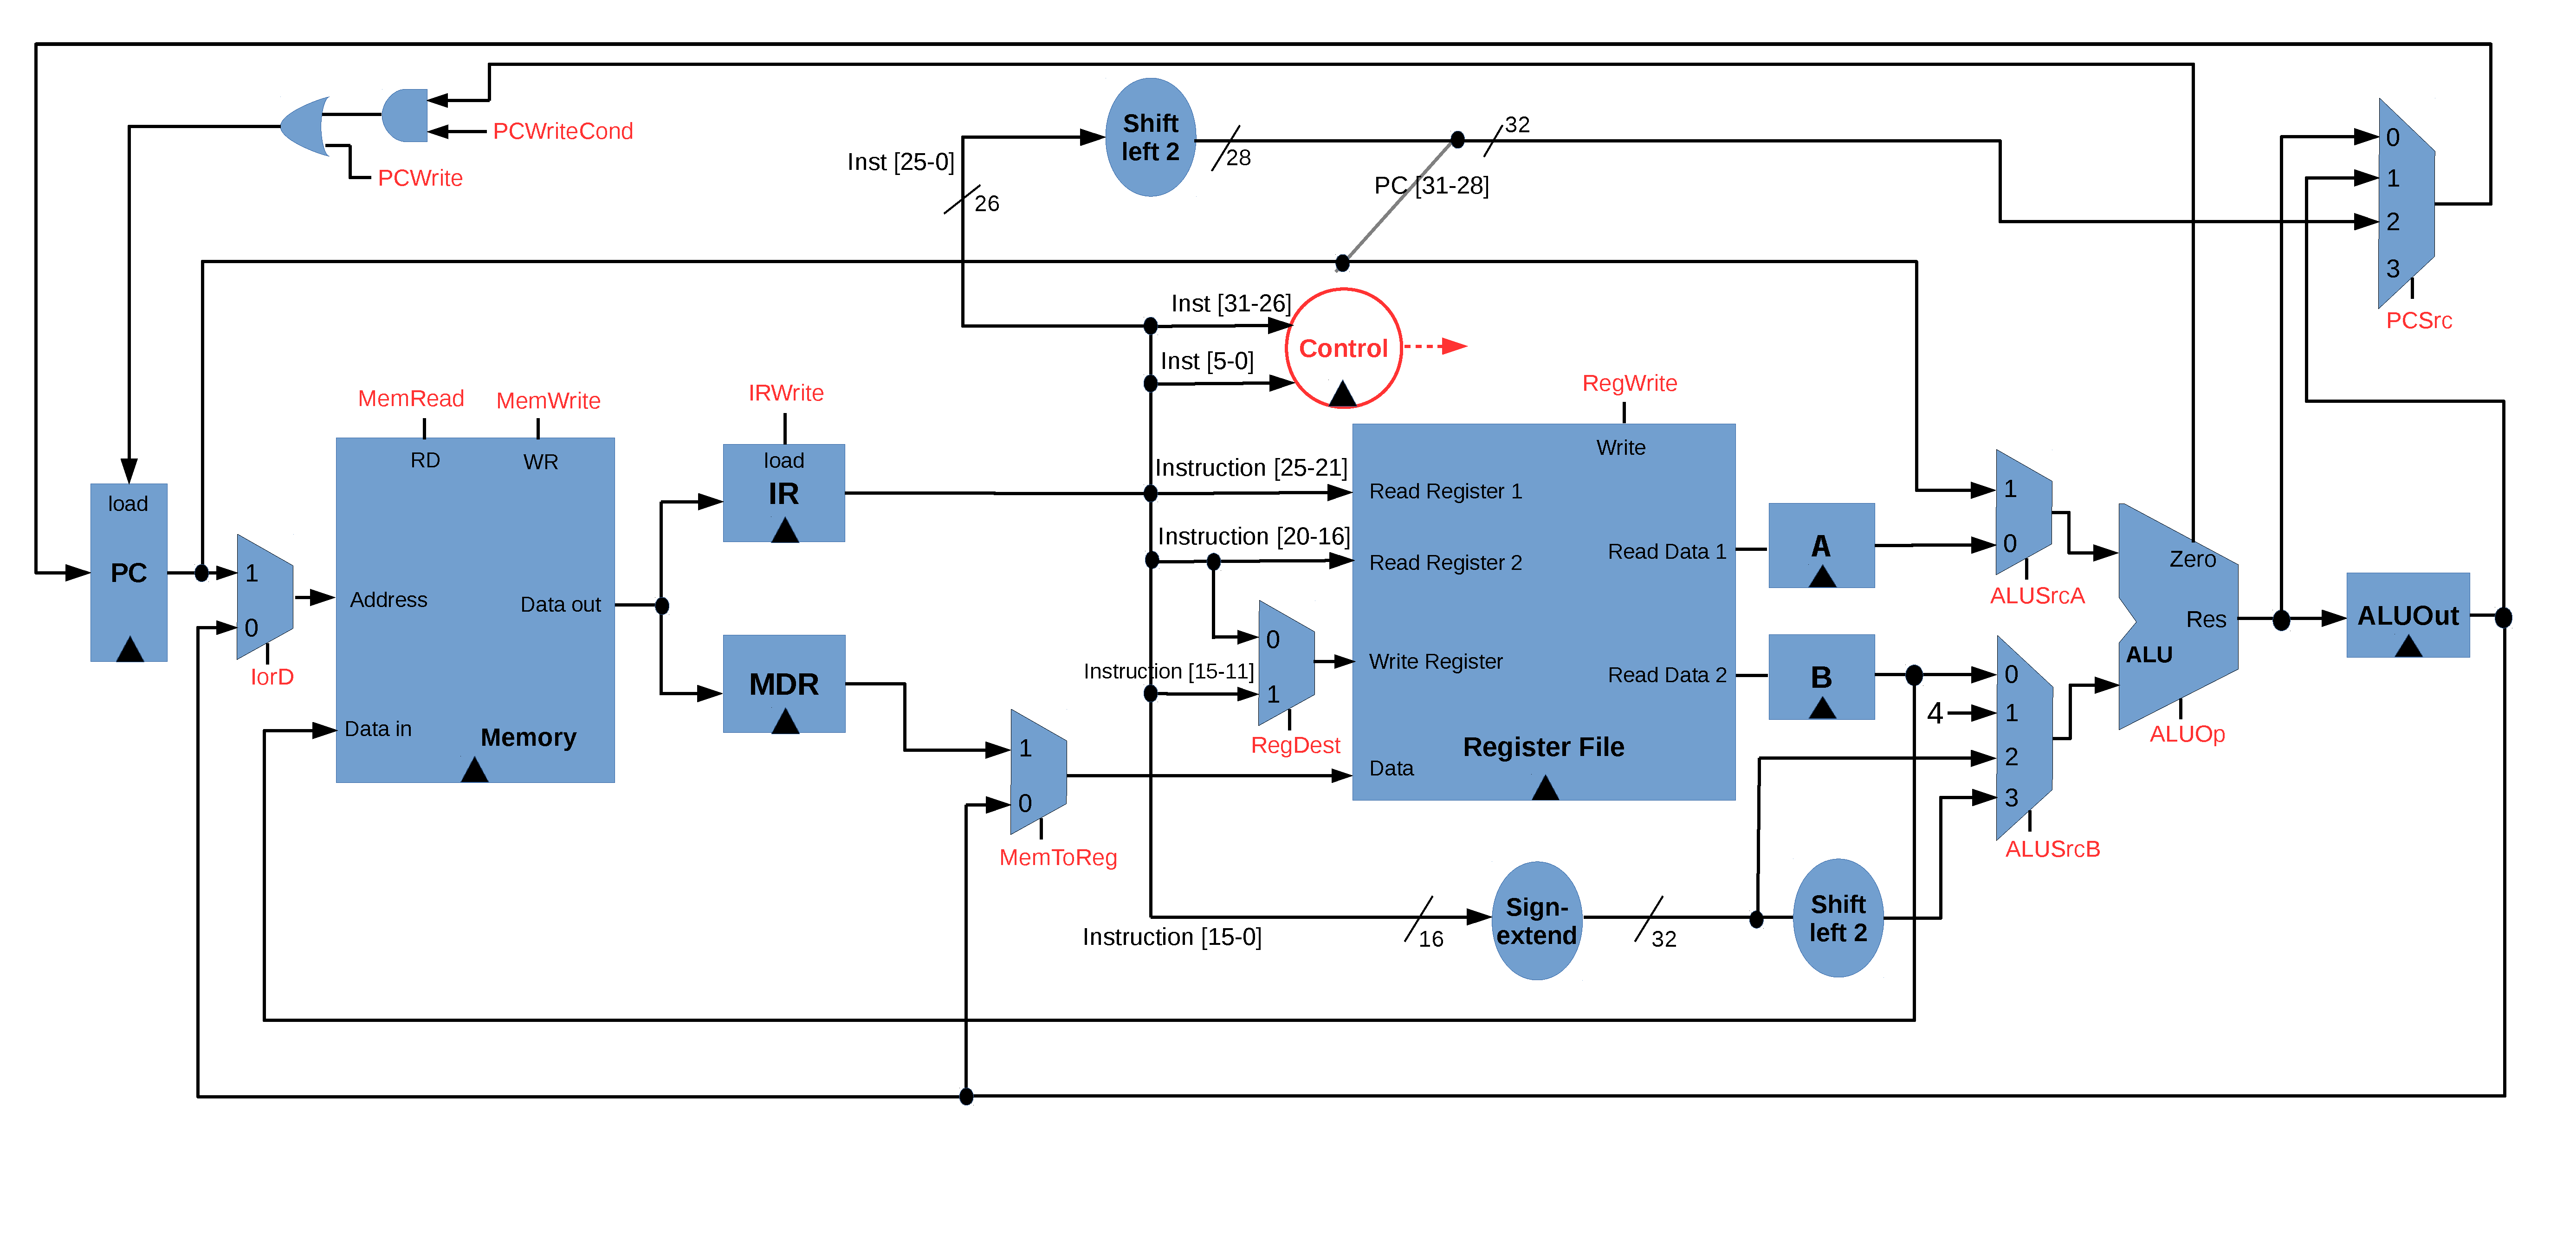
\includegraphics[width=13cm]{complete_multi_cycle.pdf}
\end{center}

\end{frame}

\begin{frame}%[fragile]
\frametitle{Instruction Fetch Stage}

\begin{center}
\hspace*{-1cm}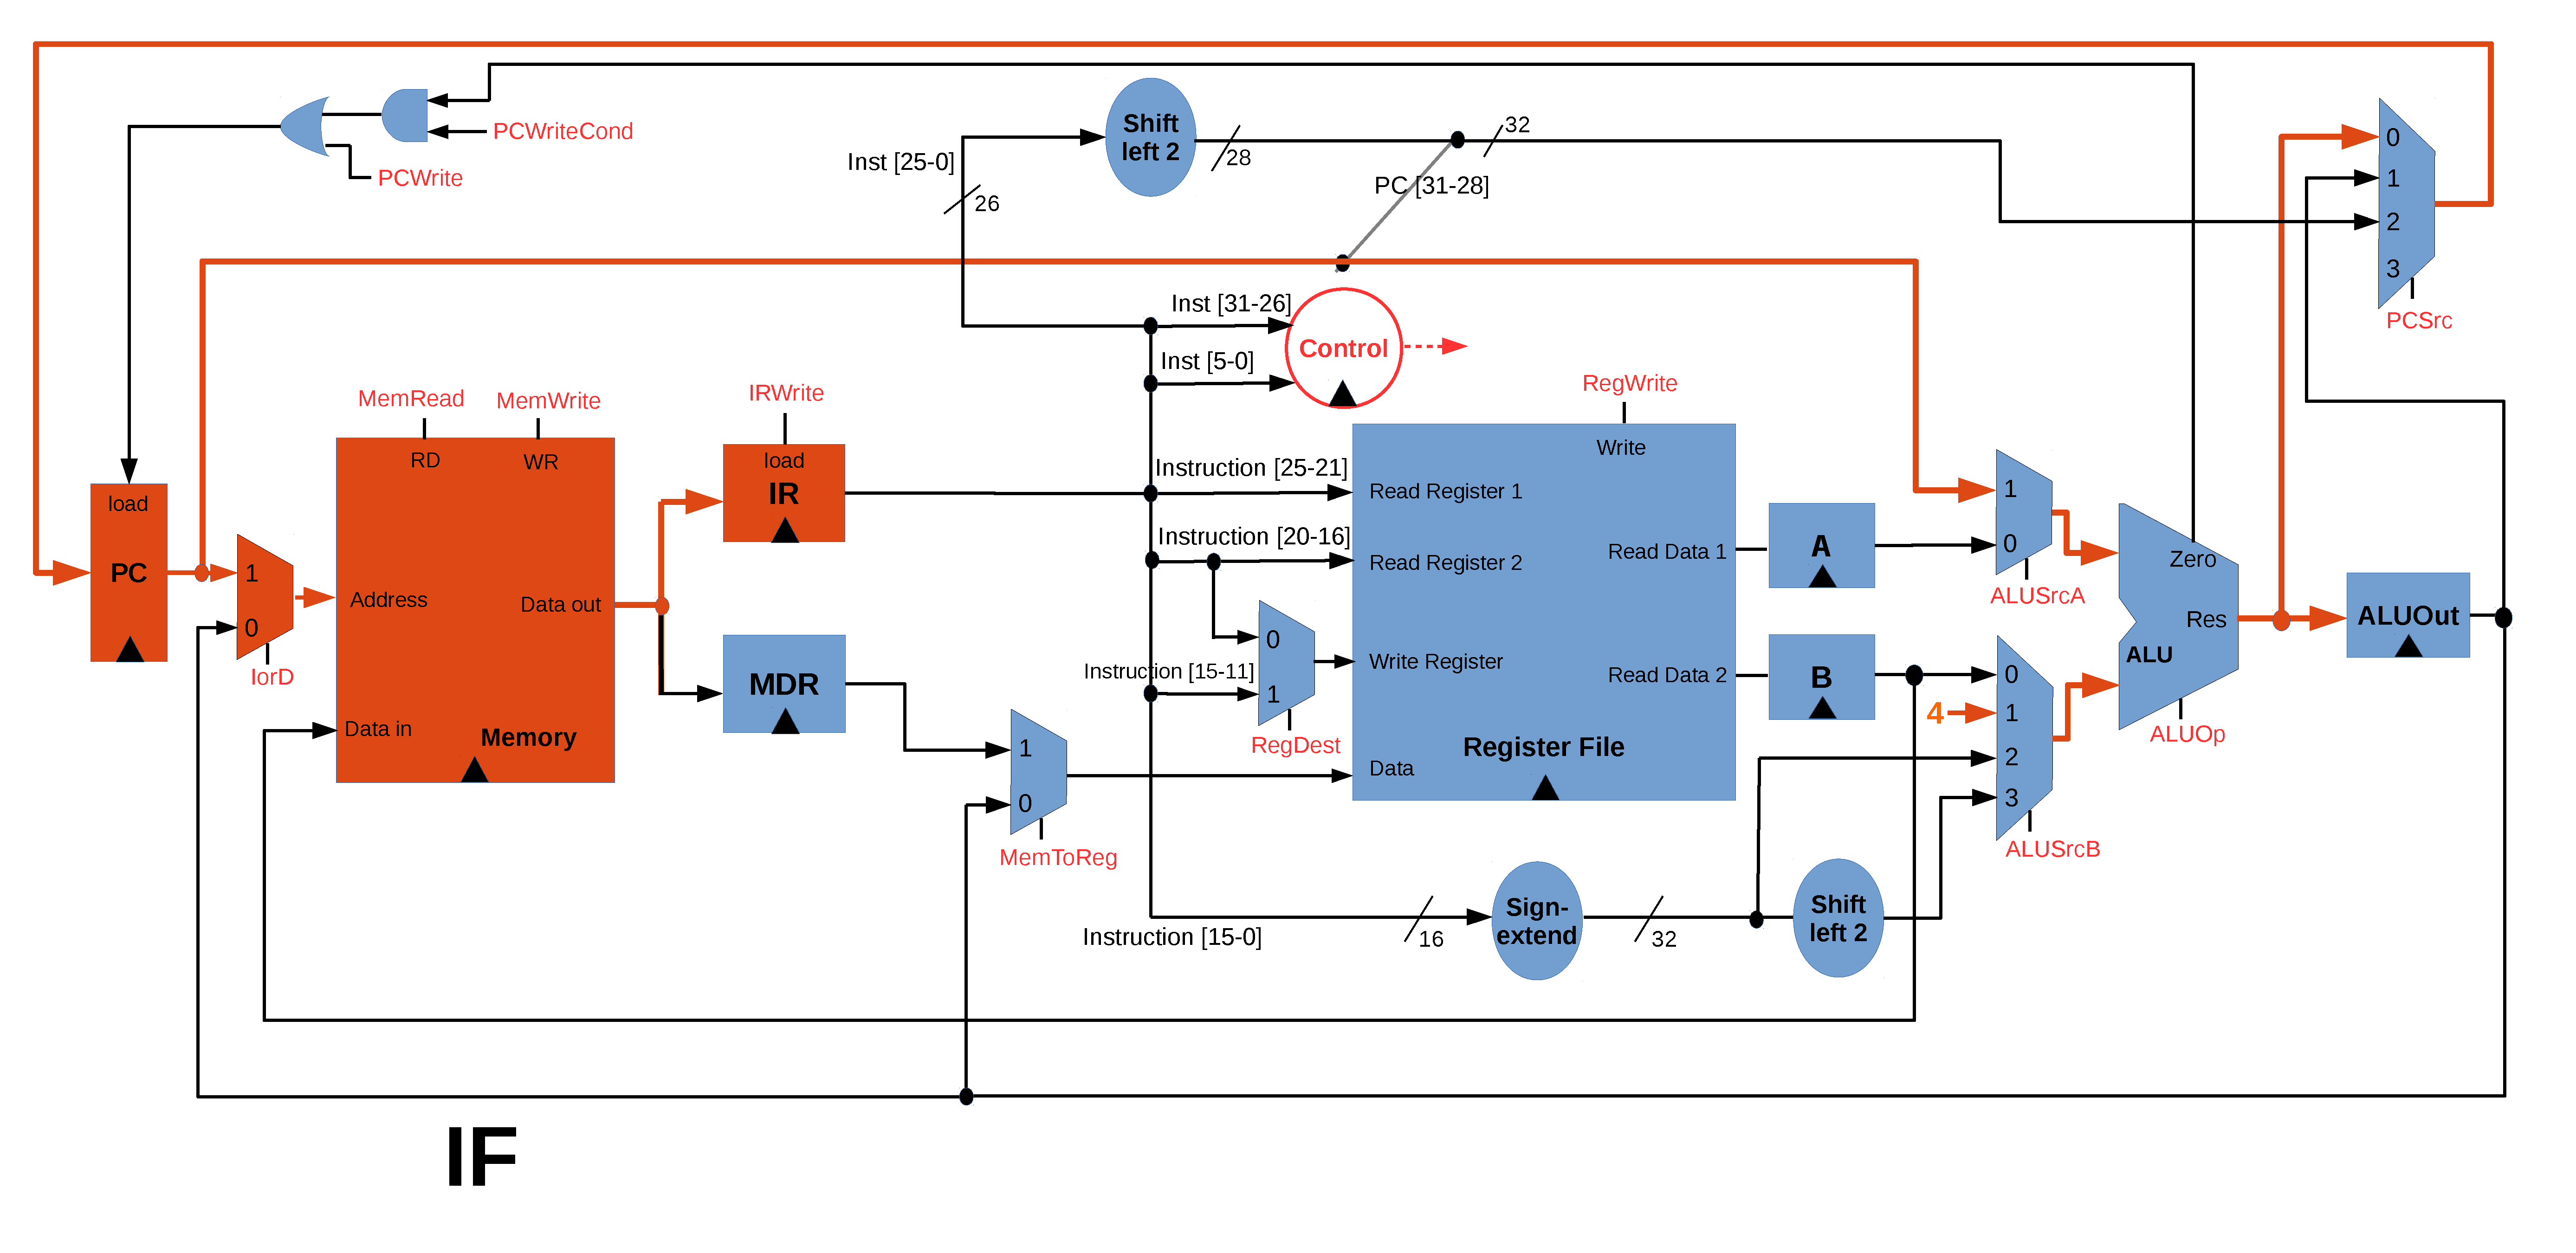
\includegraphics[width=13cm]{complete_multi_cycle_stage1.pdf}
\end{center}

\end{frame}

\begin{frame}%[fragile]
\frametitle{Instruction Decode Stage}

\begin{center}
\hspace*{-1cm}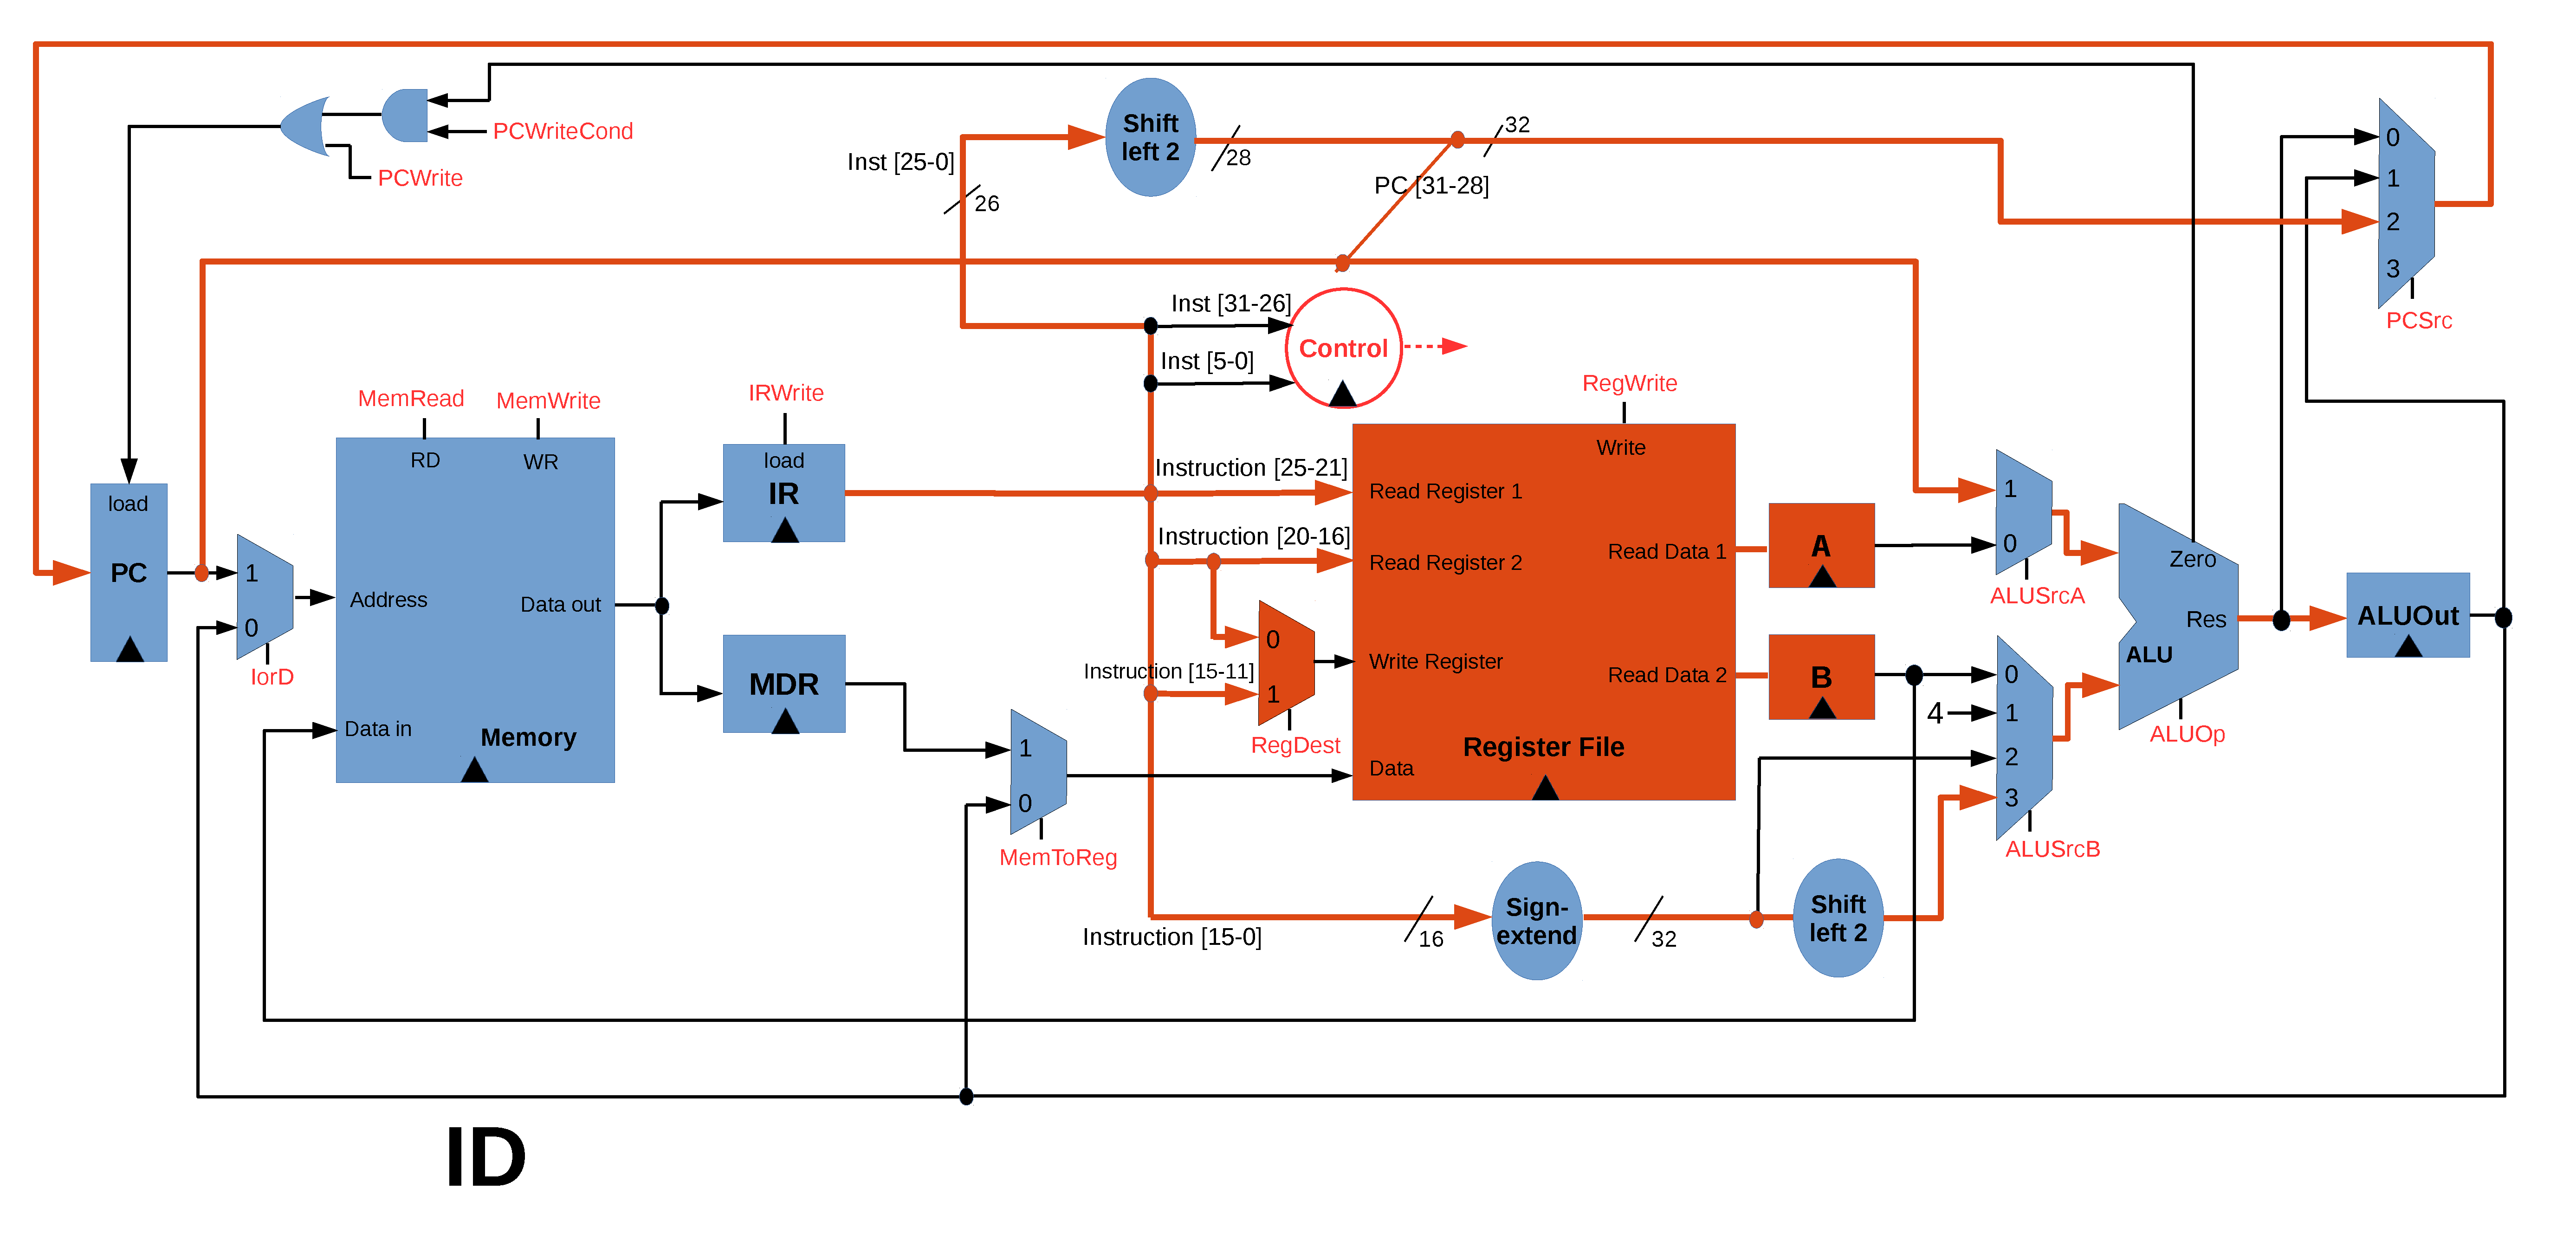
\includegraphics[width=13cm]{complete_multi_cycle_stage2.pdf}
\end{center}

\end{frame}

\begin{frame}%[fragile]
\frametitle{Execute Stage}

\begin{center}
\hspace*{-1cm}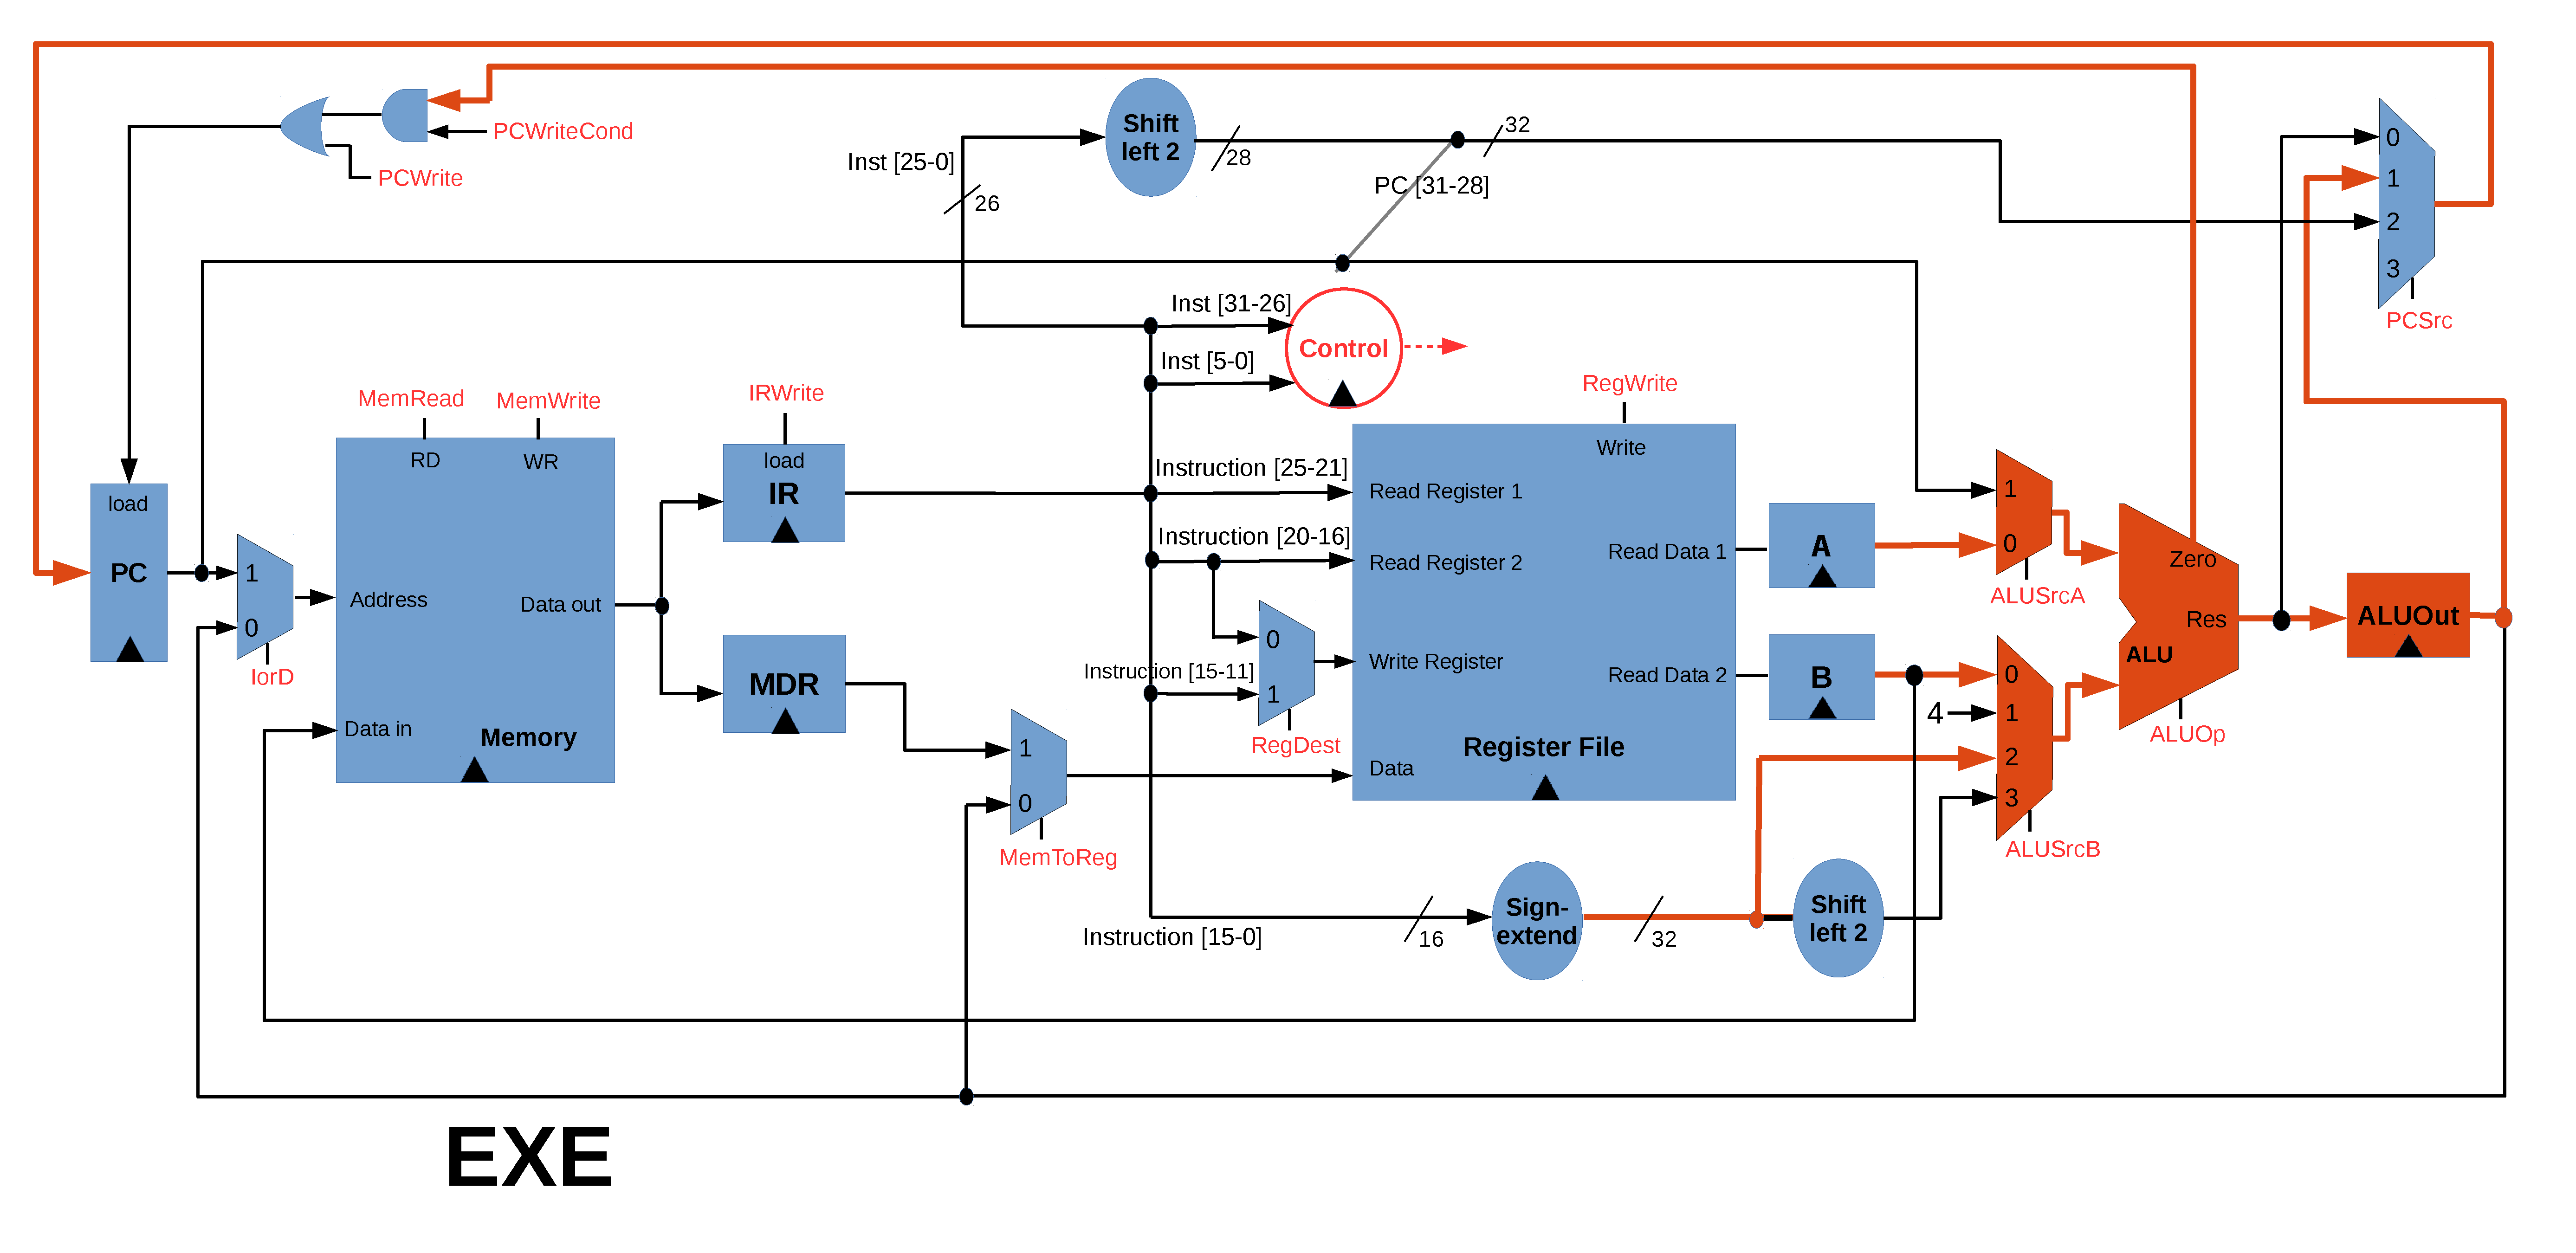
\includegraphics[width=13cm]{complete_multi_cycle_stage3.pdf}
\end{center}

\end{frame}

\begin{frame}%[fragile]
\frametitle{Memory Stage}

\begin{center}
\hspace*{-1cm}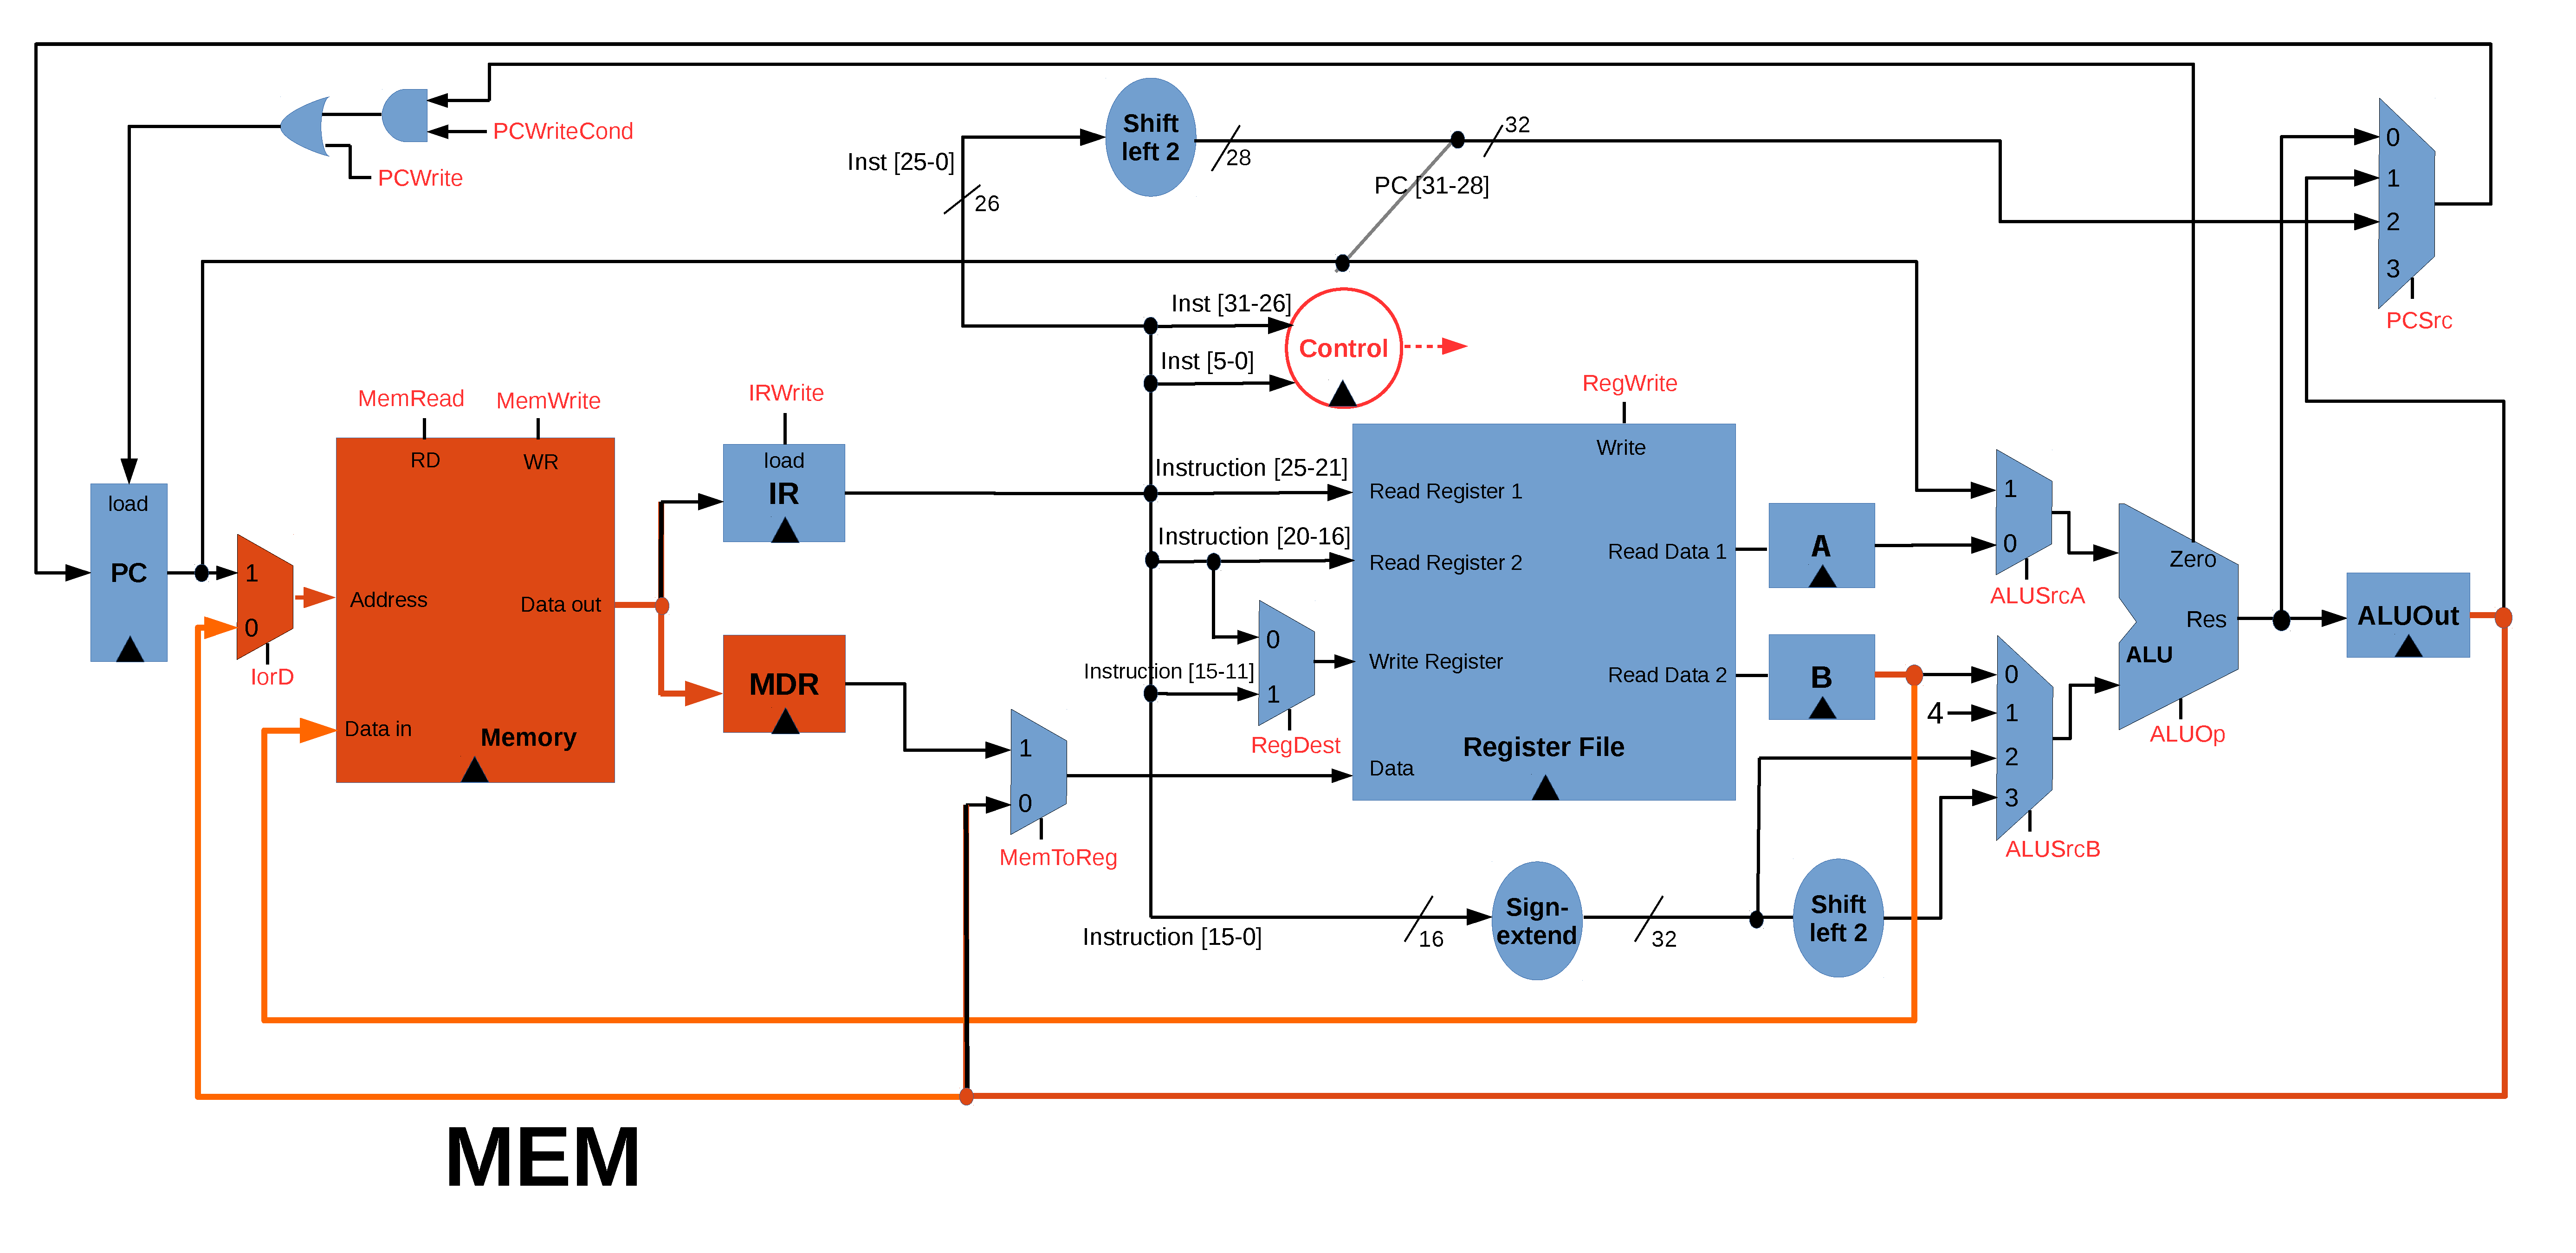
\includegraphics[width=13cm]{complete_multi_cycle_stage4.pdf}
\end{center}

\end{frame}

\begin{frame}%[fragile]
\frametitle{Write Back Stage}

\begin{center}
\hspace*{-1cm}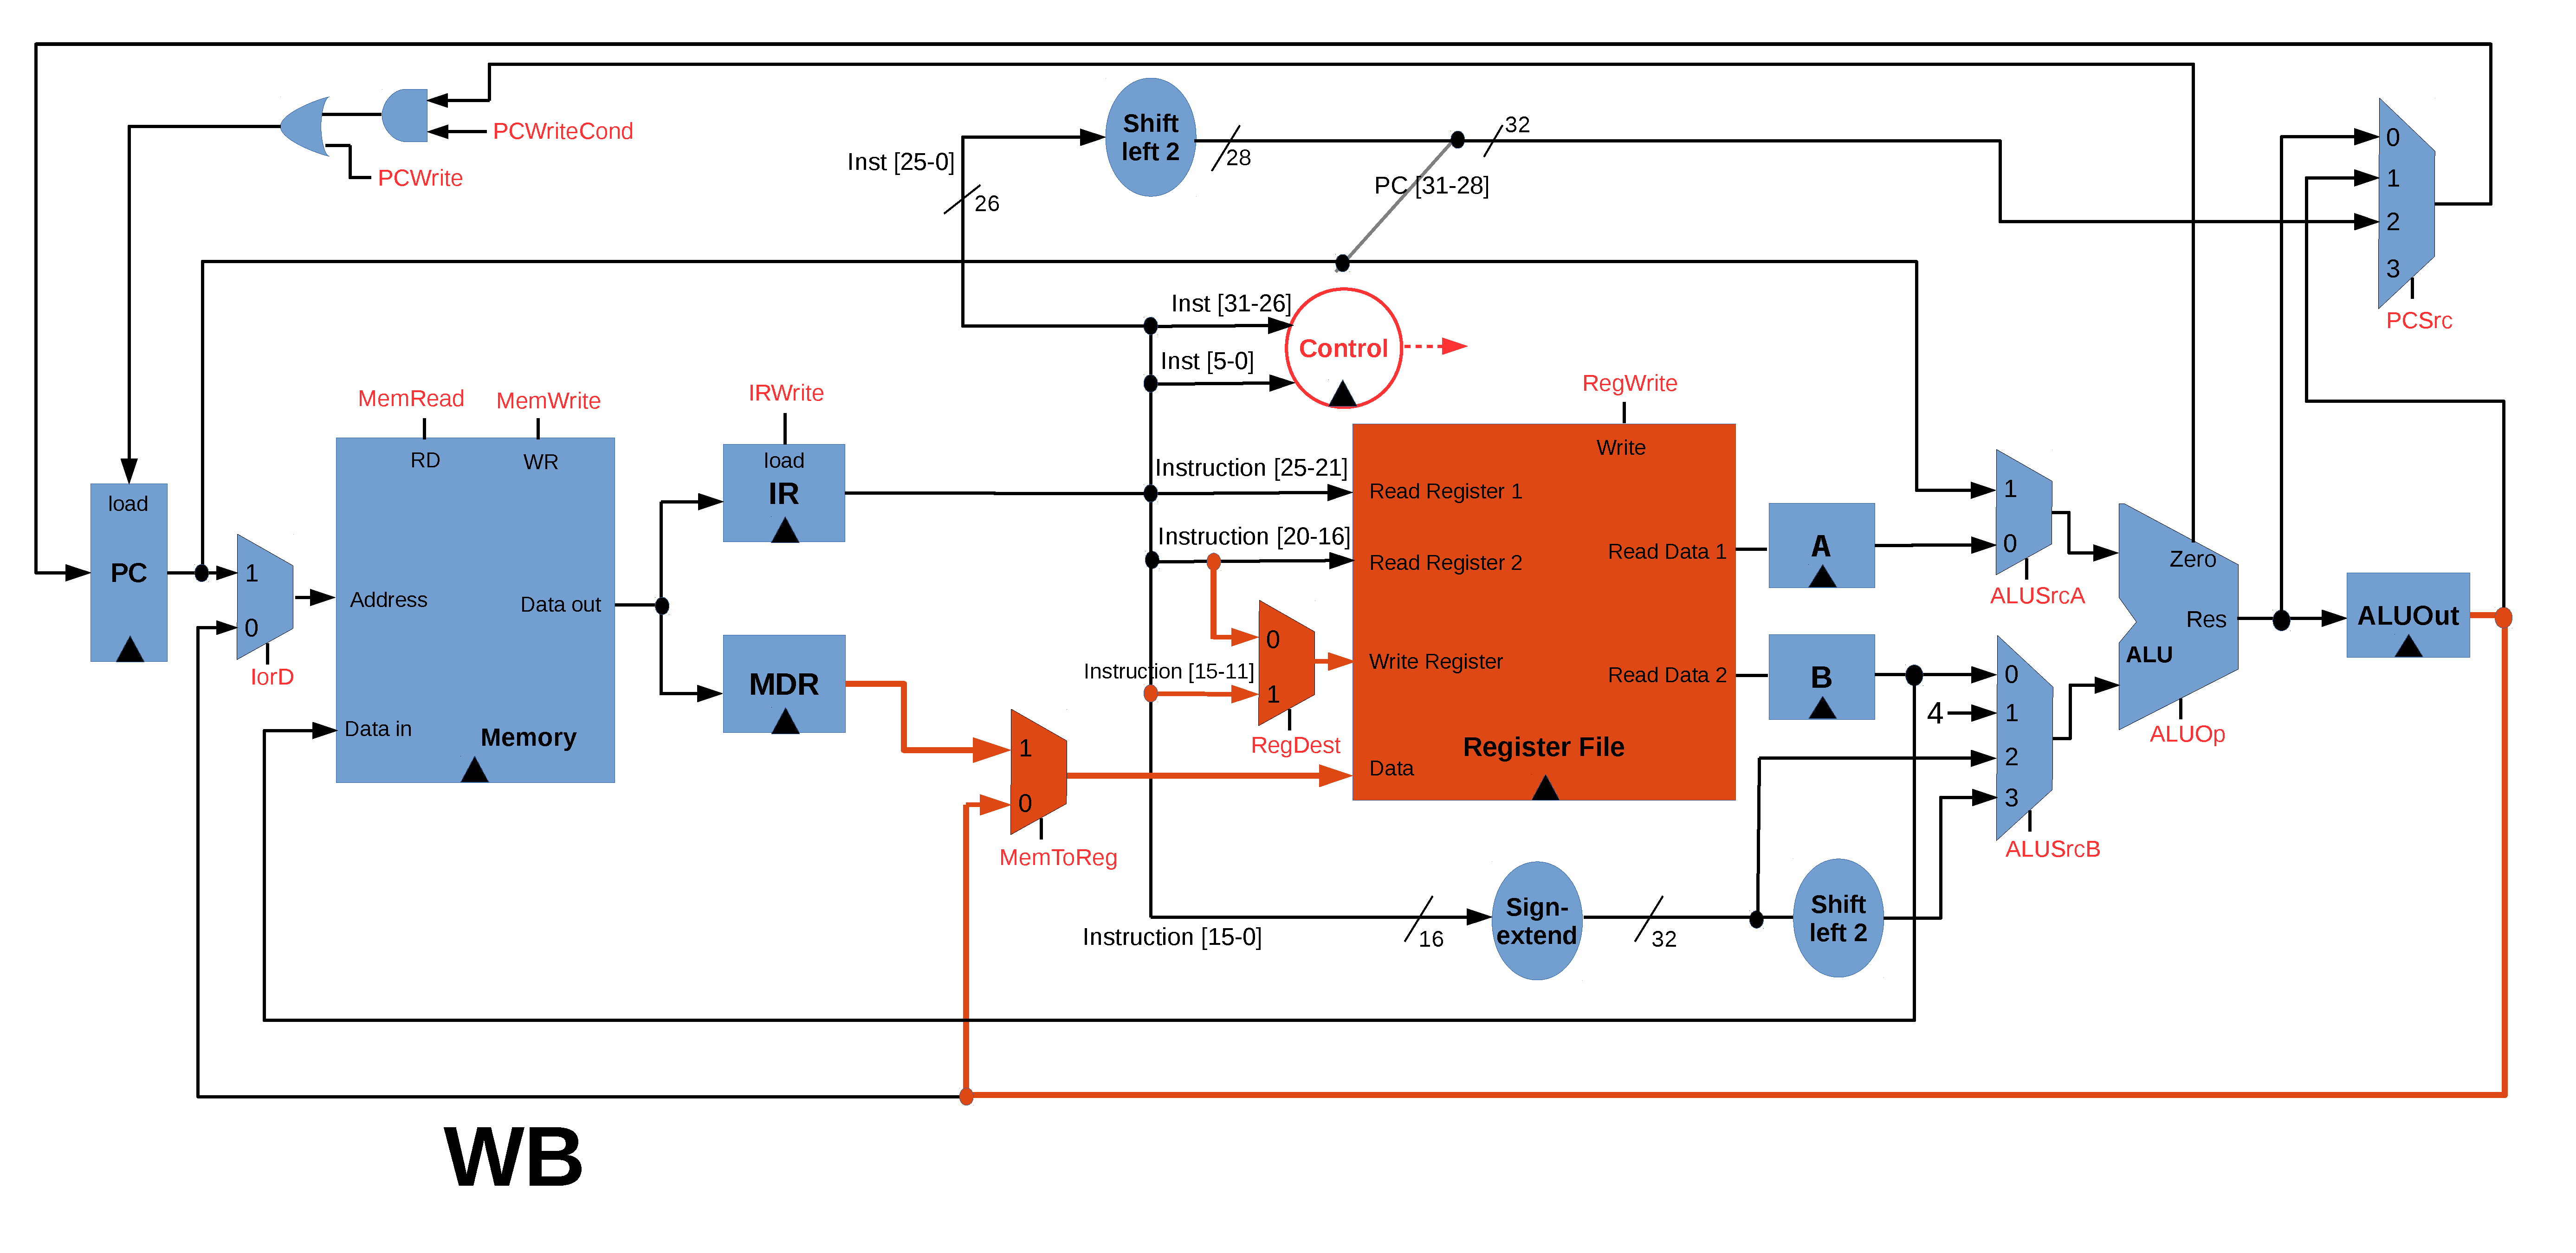
\includegraphics[width=13cm]{complete_multi_cycle_stage5.pdf}
\end{center}

\end{frame}


\section{Pipelining}

\subsection{Overview}

\begin{frame}%[fragile]
\frametitle{Pipelining}

\begin{itemize}

\item Pipelining is an implementation technique in which multiple instructions are overlapped in execution.

  \vspace{0.2cm}

\item It takes advantage of parallelism that exists among the actions needed to execute an instruction.

  \vspace{0.2cm}

\item It is a key technique to make fast CPUs.

  \vspace{0.2cm}

\item Each instruction will go through the five stages (\textcolor{blue}{IF}, \textcolor{blue}{ID}, \textcolor{blue}{EXE},
  \textcolor{blue}{MEM} and \textcolor{blue}{WB}). An instruction can do nothing in a stage.

  \vspace{0.2cm}

\item The key point is that one instruction can begin before the end of the preeceding one, contrary to the single or multi-cycle
  implementation.

\end{itemize}

\end{frame}

\begin{frame}%[fragile]
\frametitle{Laundry Example}

\tiny
(From Computer Organization and Design. Patterson and Hennessy)

\begin{center}
  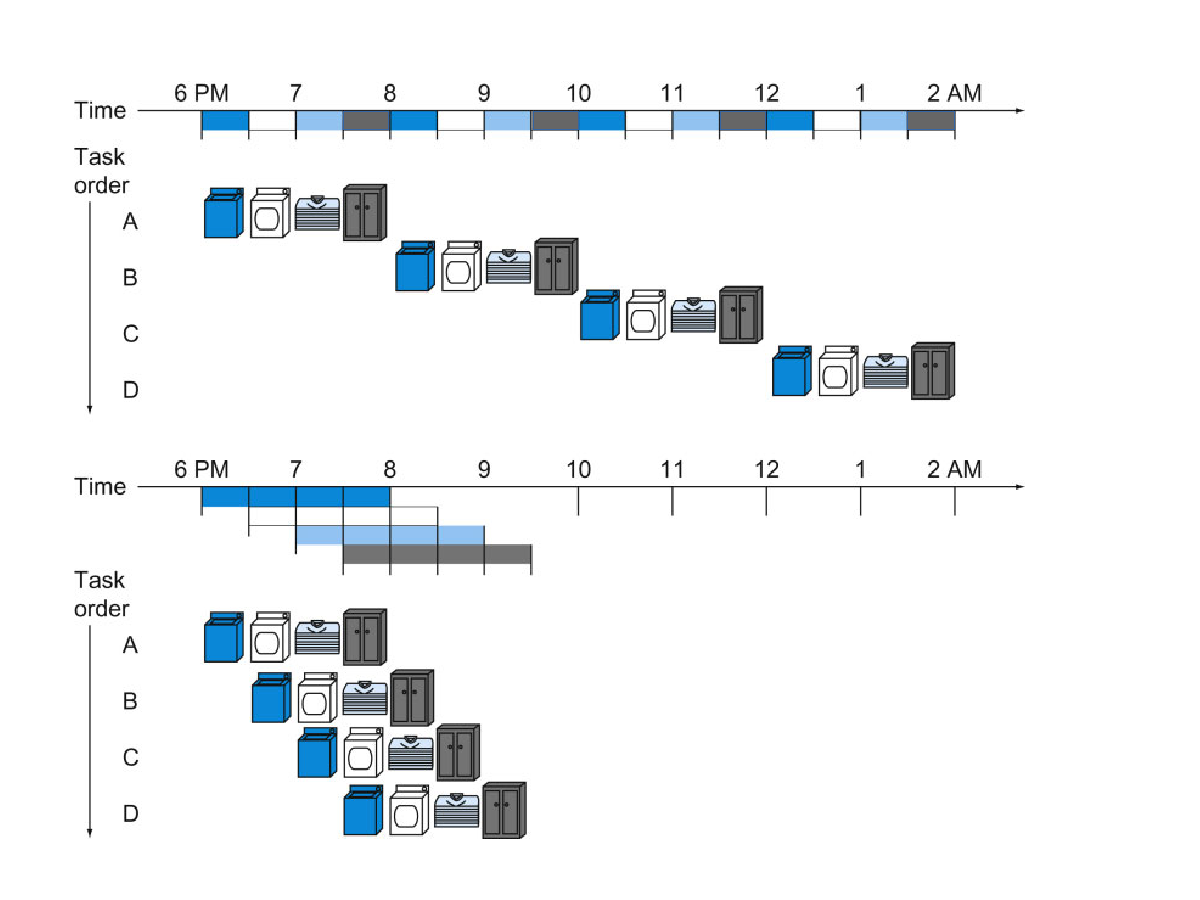
\includegraphics[width=9cm]{pipelining_laundry.pdf}
\end{center}

\end{frame}


\subsection{Timing Comparison}

\begin{frame}[fragile]
\frametitle{Comparing Single-Cycle, Multi-Cycle and Pipelining}

We will compare the behavior of the single-cycle, multi-cycle
and pipelining architecture on the following program:

\vspace{0.3cm}

\scriptsize

\begin{lstlisting}
main:
        lw  $t0,  0($s1)
        lw  $t1,  4($s1)
        lw  $t2,  8($s1)
        lw  $t3, 12($s1)
        add $t4, $t0, $t1
        add $t5, $t2, $t3
        add $t6, $t4, $t5
        sw  $t6, 16($s1)
        # ...
\end{lstlisting}

\end{frame}

\begin{frame}%[fragile]
\frametitle{Comparing Single-Cycle, Multi-Cycle and Pipelining}

\begin{center}
\hspace*{-1cm}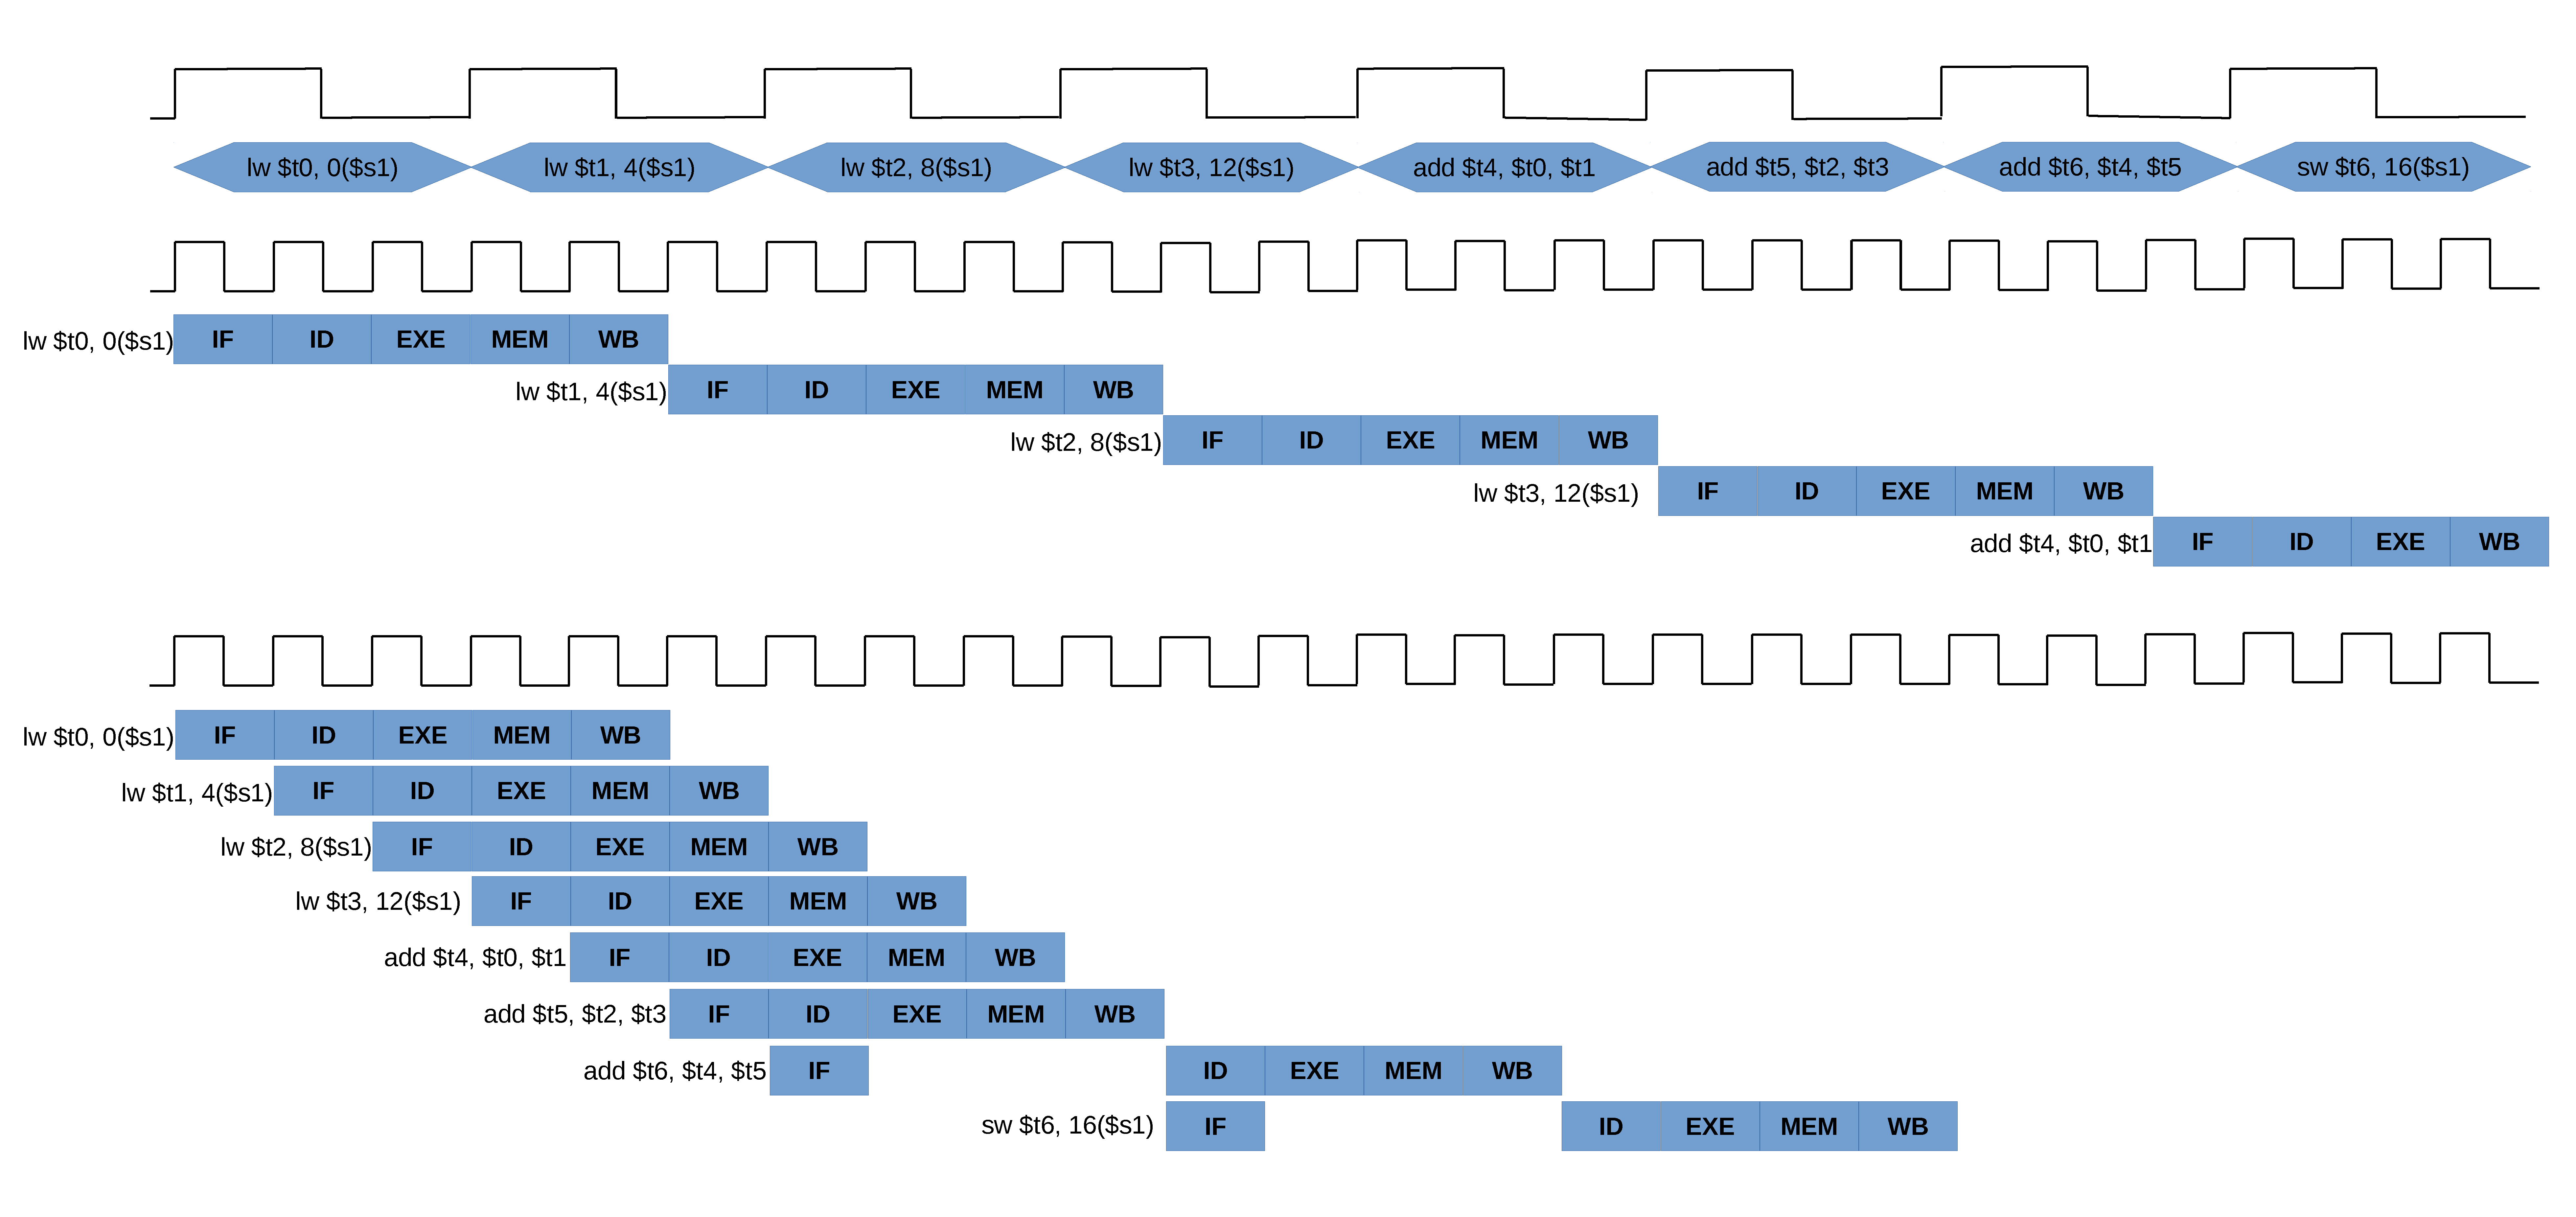
\includegraphics[width=12.8cm]{sc_mc_pipelining.pdf}
\end{center}

\end{frame}

\begin{frame}[fragile]
\frametitle{\exo}

\scriptsize

We add the following highlighted instructions to the program. Can you speed-up
the program by reordering instructions? How much do you gain?

\vspace{0.3cm}

\begin{lstlisting}[linebackgroundcolor={\lstcolorlines{10,11,12,13,14,15}}]
main:
        lw   $t0,  0($s1)
        lw   $t1,  4($s1)
        lw   $t2,  8($s1)
        lw   $t3, 12($s1)
        add  $t4, $t0, $t1
        add  $t5, $t2, $t3
        add  $t6, $t4, $t5
        sw   $t6, 16($s1)
        lw   $t0,  0($s2)
        lw   $t1,  4($s2)
        lw   $t2,  8($s2)
        addi $t0, $t9, 42
        addi $t1, $t9, 100
        addi $t2, $t9, 2017
        # ...
\end{lstlisting}

\end{frame}

\ifanswers

\begin{frame}[fragile]
\frametitle{Solution}

\begin{center}
\hspace*{-1cm}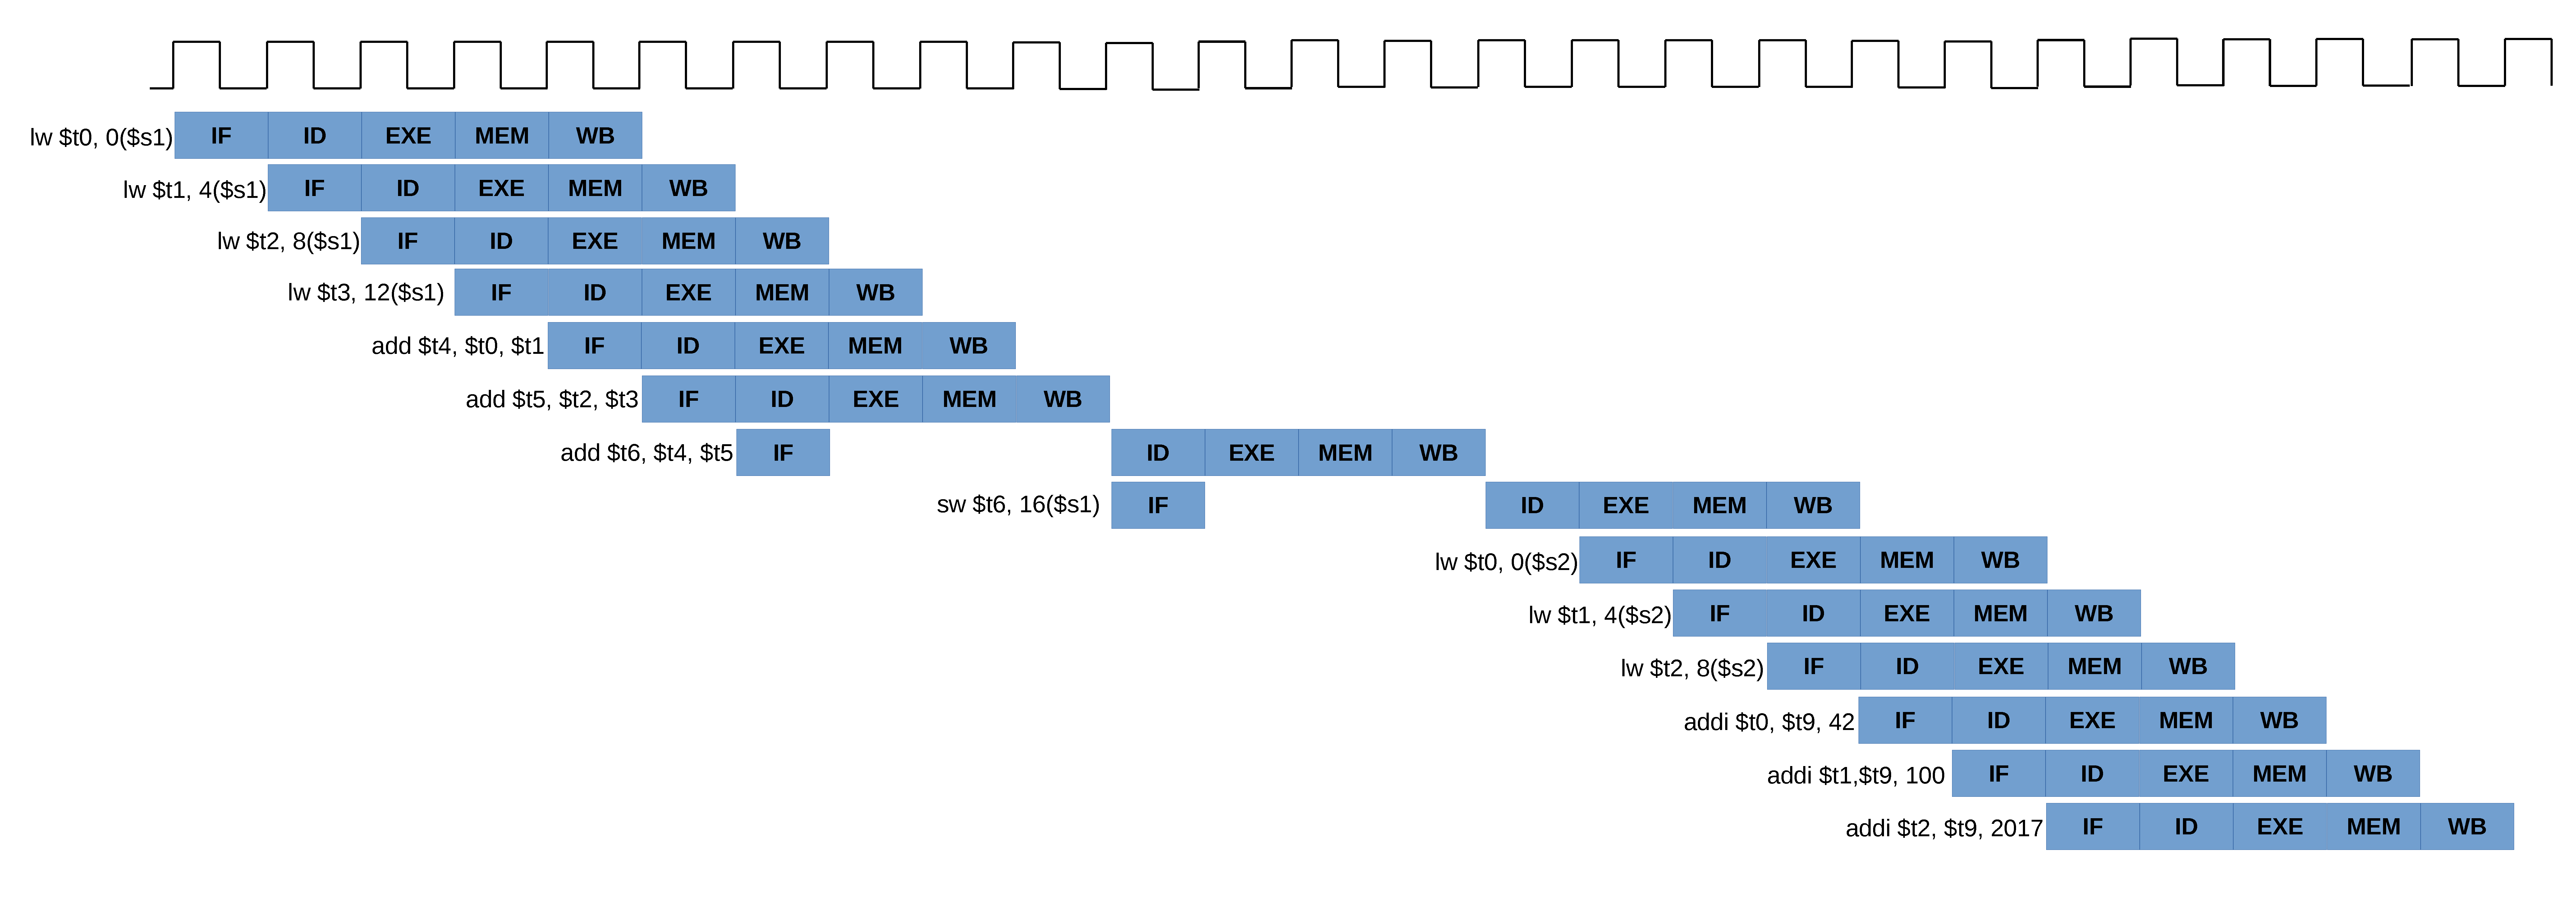
\includegraphics[width=12.8cm]{pipelining_reorder_exo1.pdf}
\end{center}

\end{frame}

\begin{frame}[fragile]
\frametitle{Solution}

\scriptsize

\begin{lstlisting}[linebackgroundcolor={\lstcolorlines{8,9,10,12,13,14}}]
main:
        lw   $t0,  0($s1)
        lw   $t1,  4($s1)
        lw   $t2,  8($s1)
        lw   $t3, 12($s1)
        add  $t4, $t0, $t1
        add  $t5, $t2, $t3
        lw   $t0,  0($s2)
        lw   $t1,  4($s2)
        lw   $t2,  8($s2)
        add  $t6, $t4, $t5
        addi $t0, $t9, 42
        addi $t1, $t9, 100
        addi $t2, $t9, 2017
        sw   $t6, 16($s1)
        # ...
\end{lstlisting}

\end{frame}

\begin{frame}[fragile]
\frametitle{Solution}

\begin{center}
\hspace*{-1cm}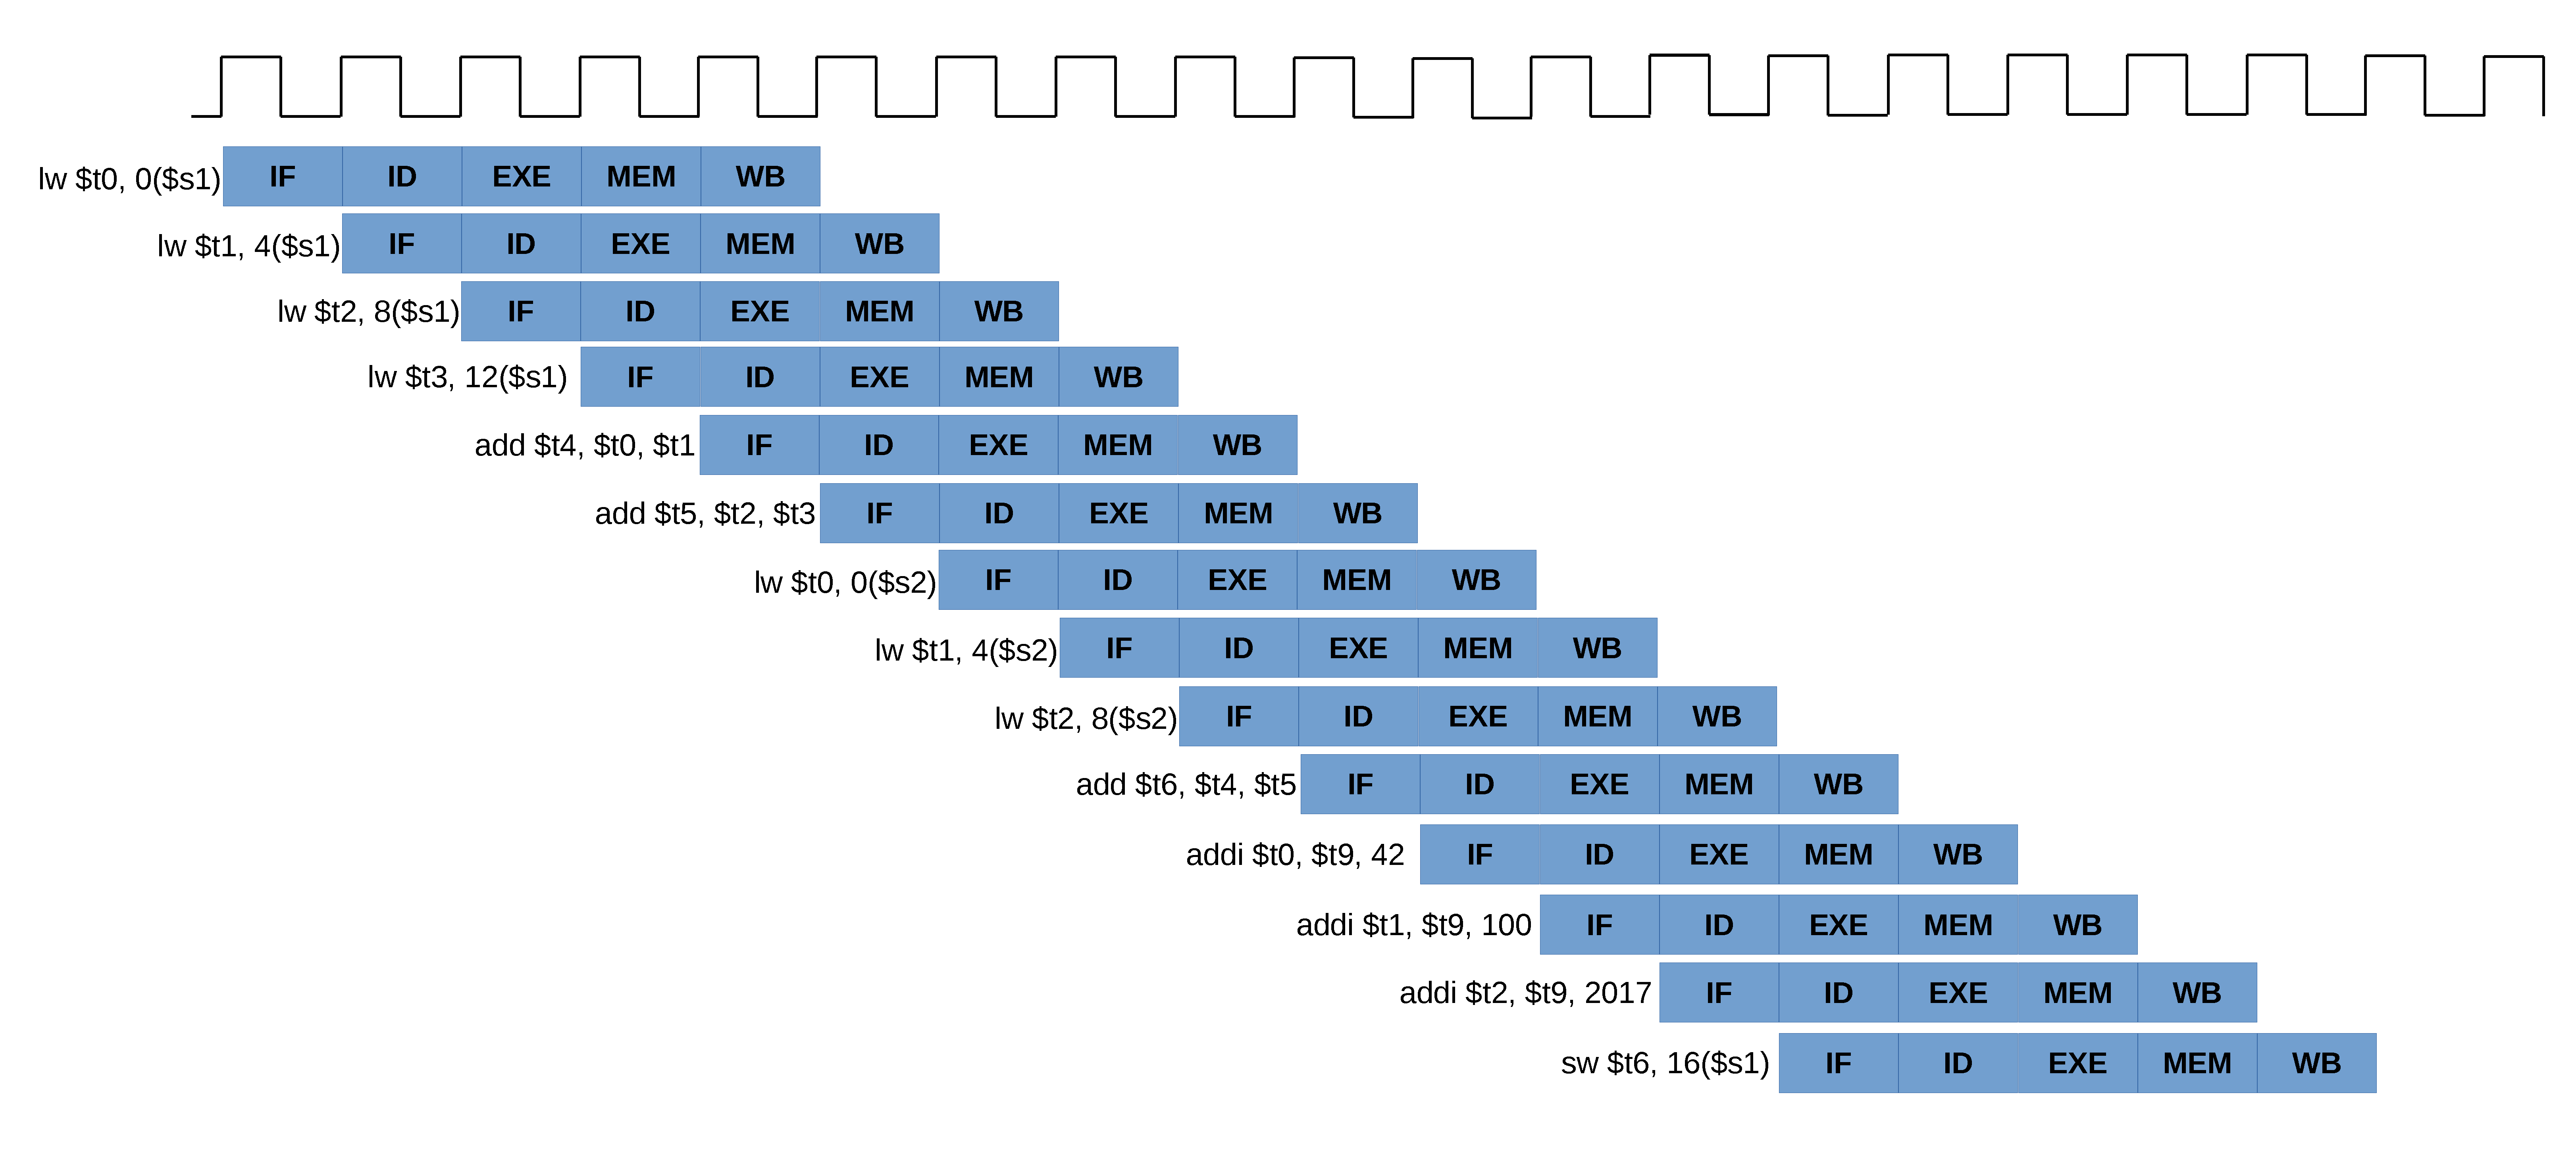
\includegraphics[width=12.8cm]{pipelining_reorder_exo2.pdf}
\end{center}

\end{frame}

\fi

\section{Interrupts}

\subsection{Interrupts and Exceptions}

\begin{frame}%[fragile]
\frametitle{Interrupts and Exceptions}


\end{frame}

\subsection{I/O Devices}

\begin{frame}%[fragile]
\frametitle{I/O Devices}

\vspace*{-0.2cm}
\begin{center}
  \hspace*{-1cm}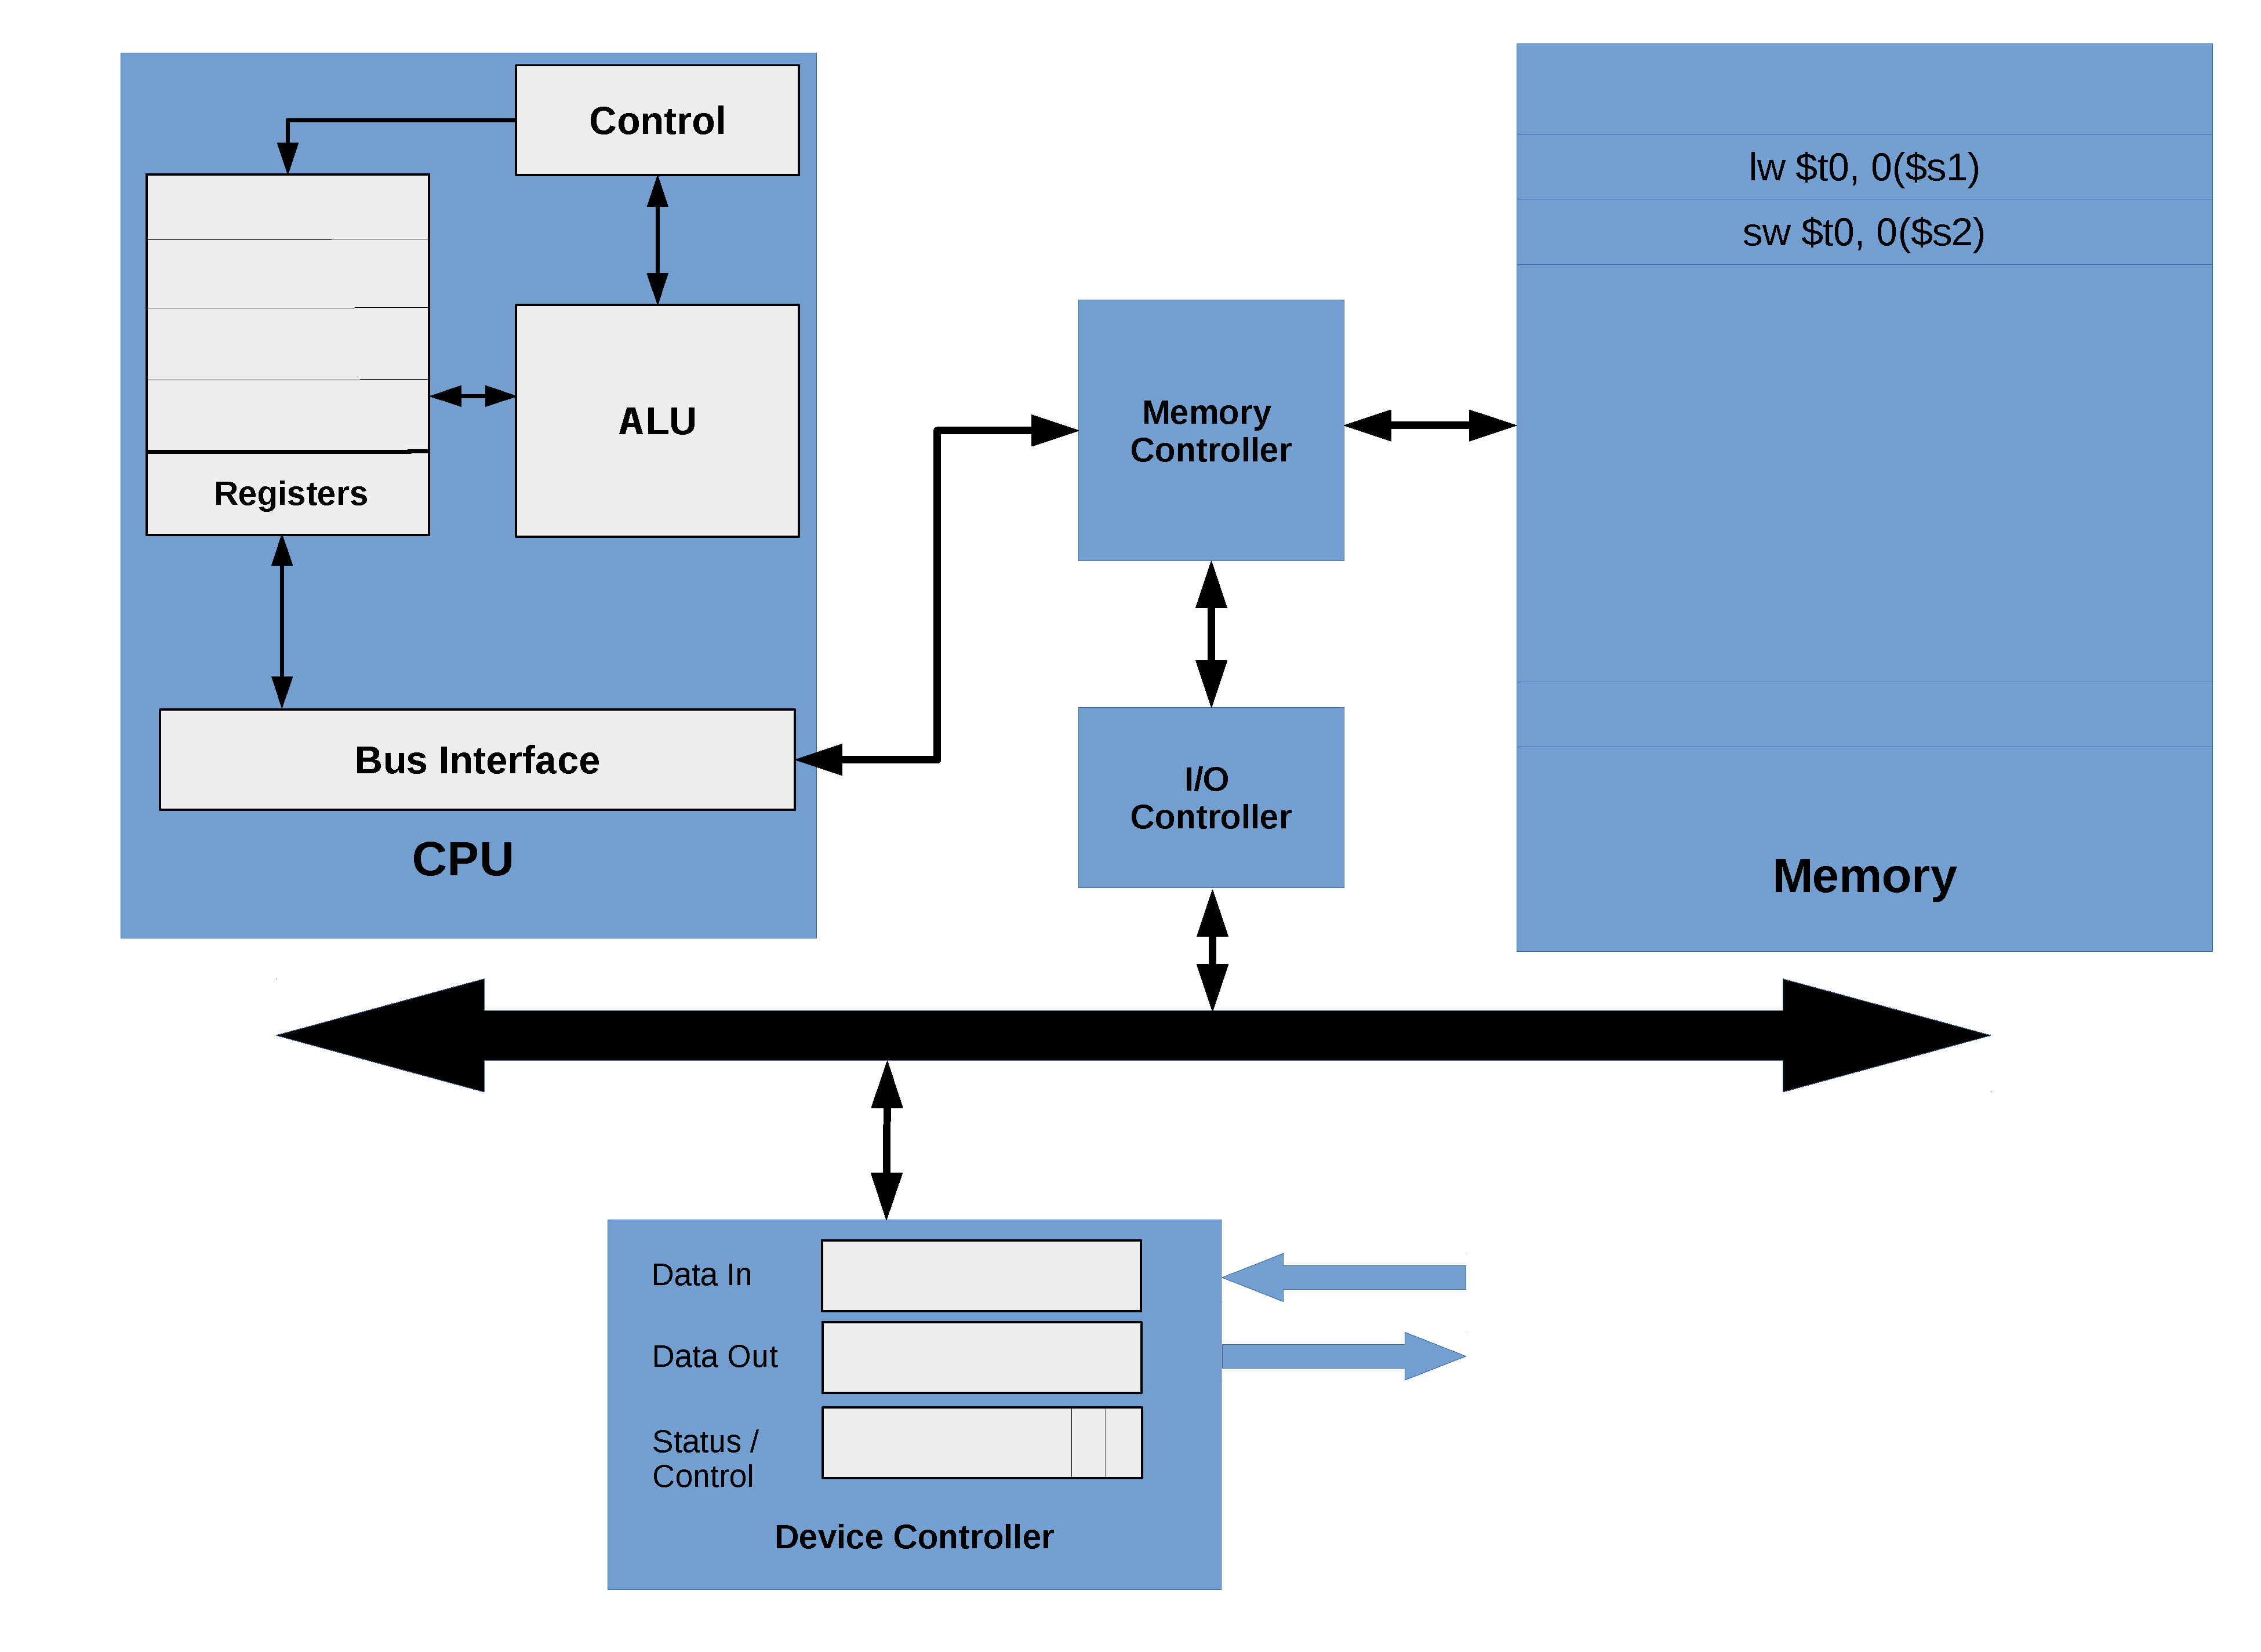
\includegraphics[width=10cm]{io_device1.pdf}
\end{center}

\end{frame}

\begin{frame}%[fragile]
\frametitle{I/O Devices}

\vspace*{-0.2cm}
\begin{center}
\hspace*{-1cm}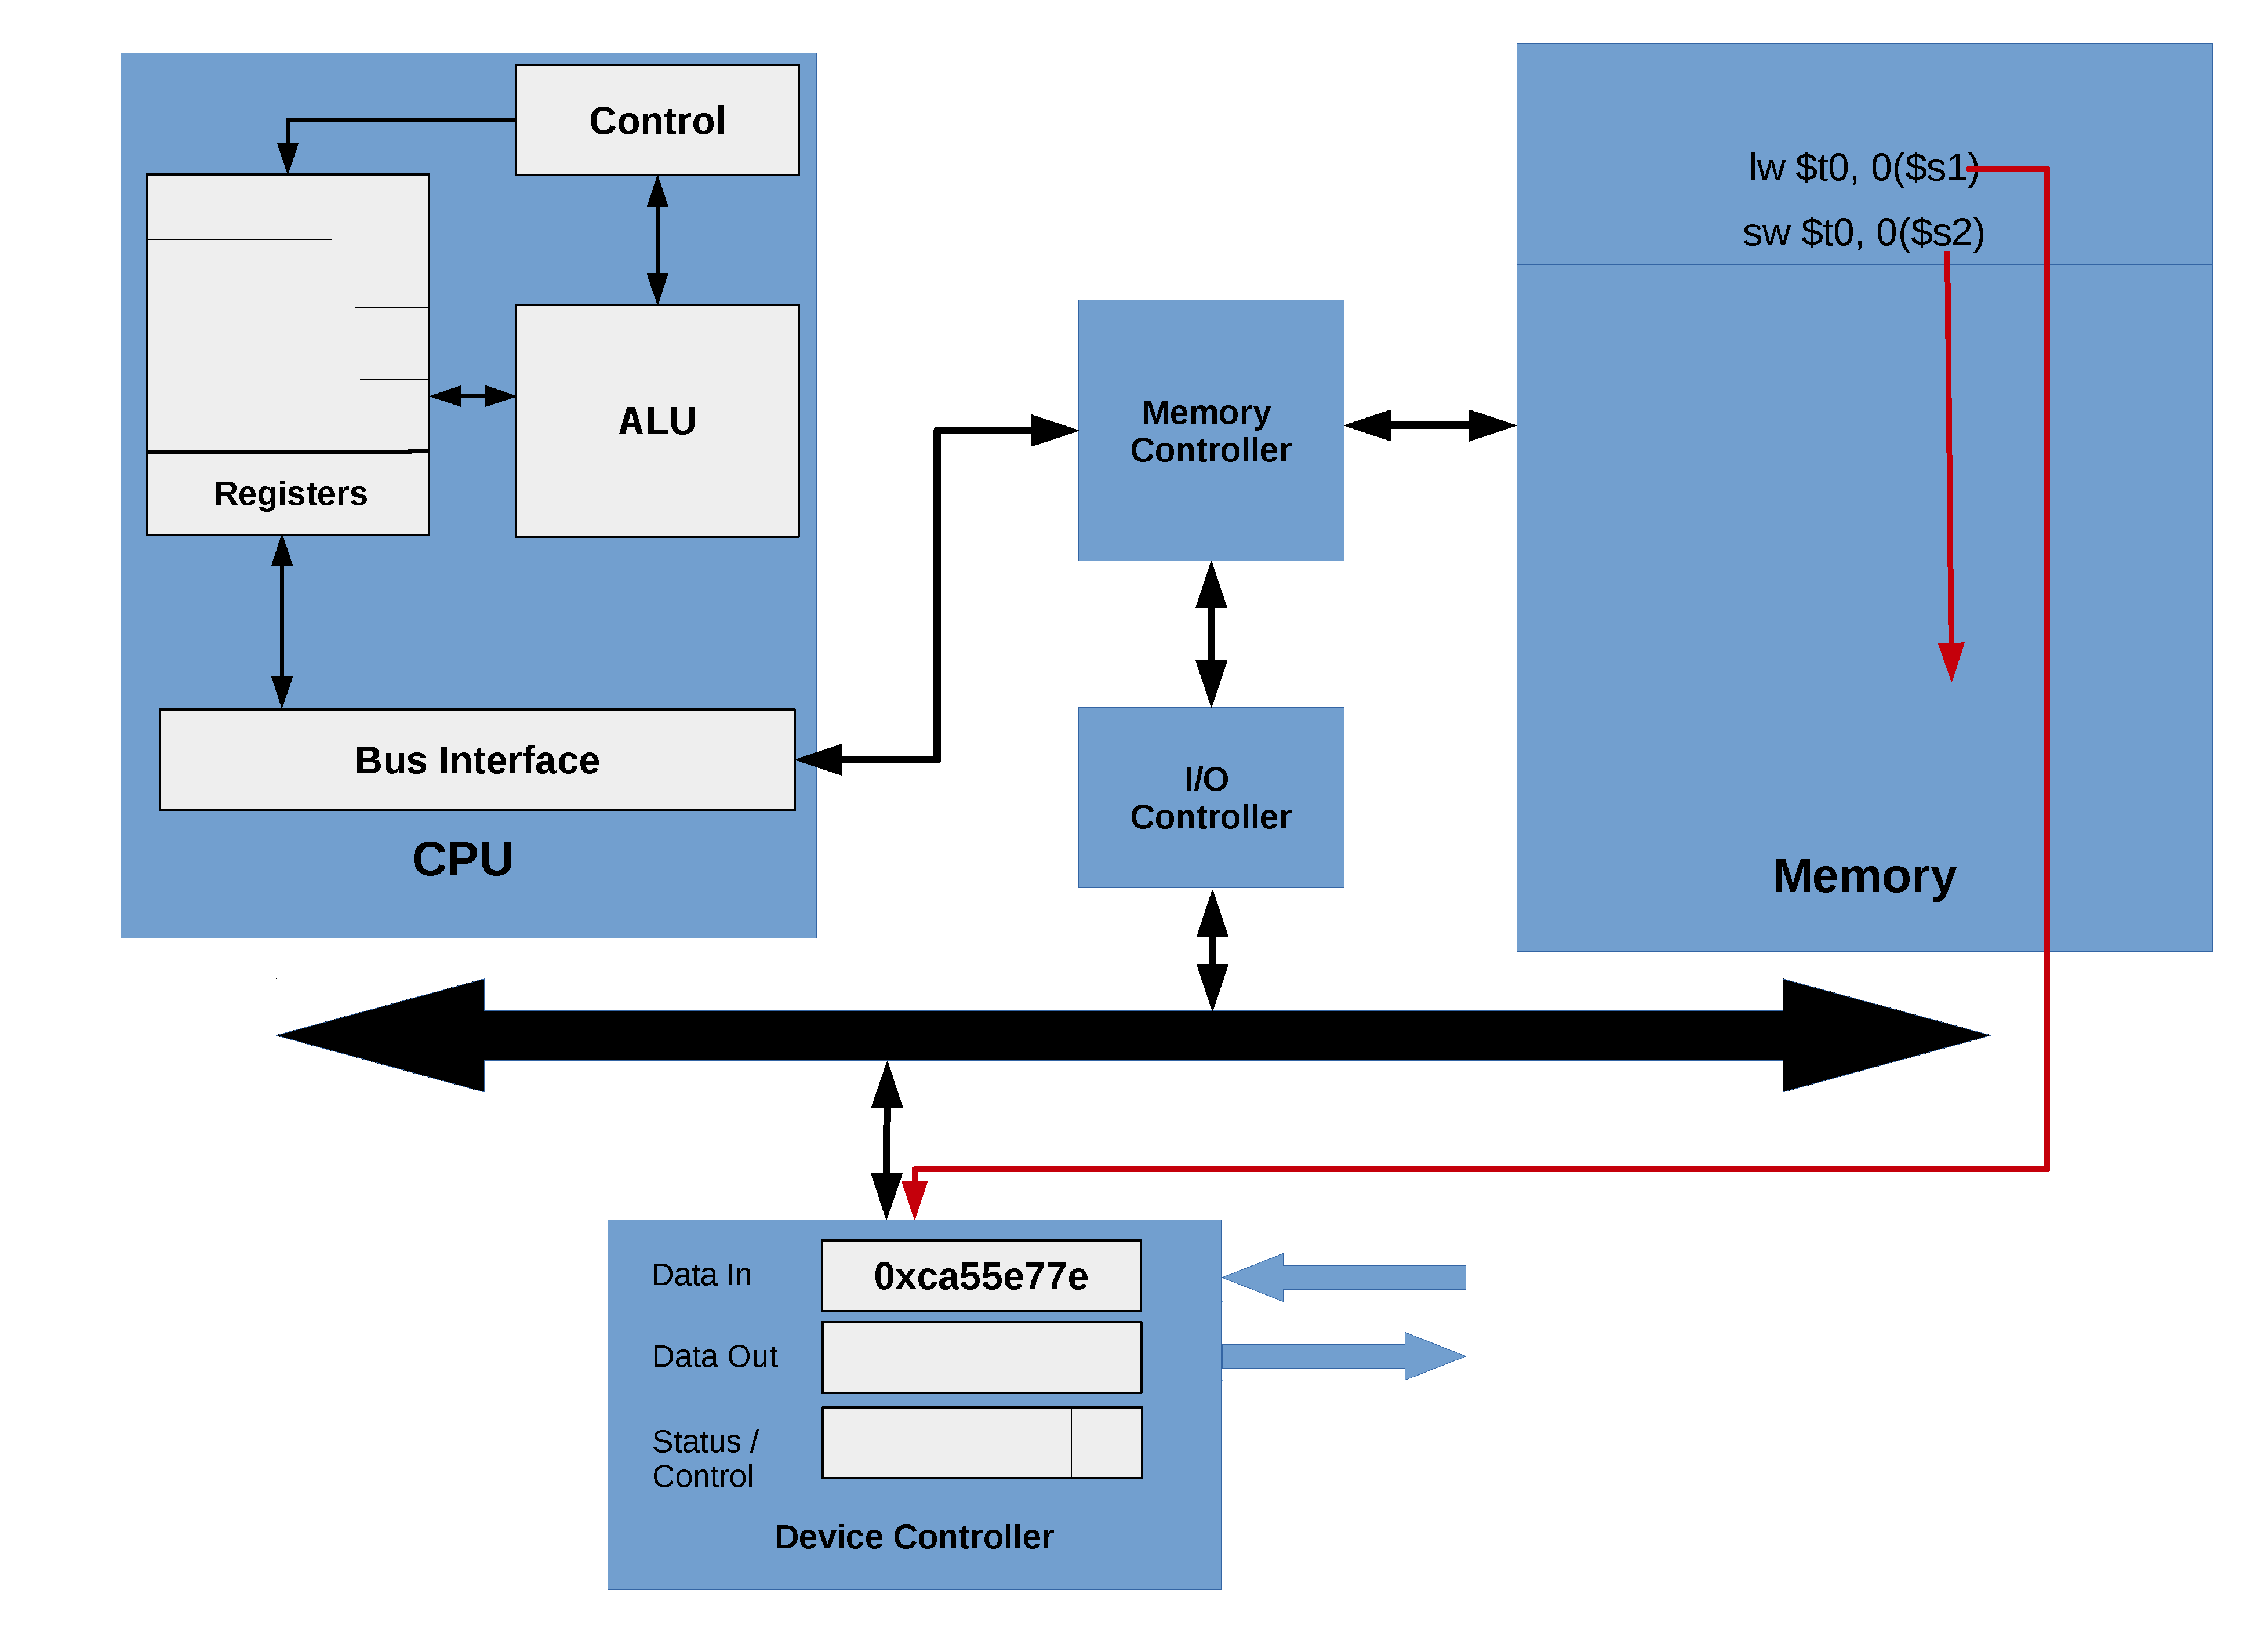
\includegraphics[width=10cm]{io_device2.pdf}
\end{center}

\end{frame}

\begin{frame}%[fragile]
\frametitle{I/O Devices}

\vspace*{-0.2cm}
\begin{center}
\hspace*{-1cm}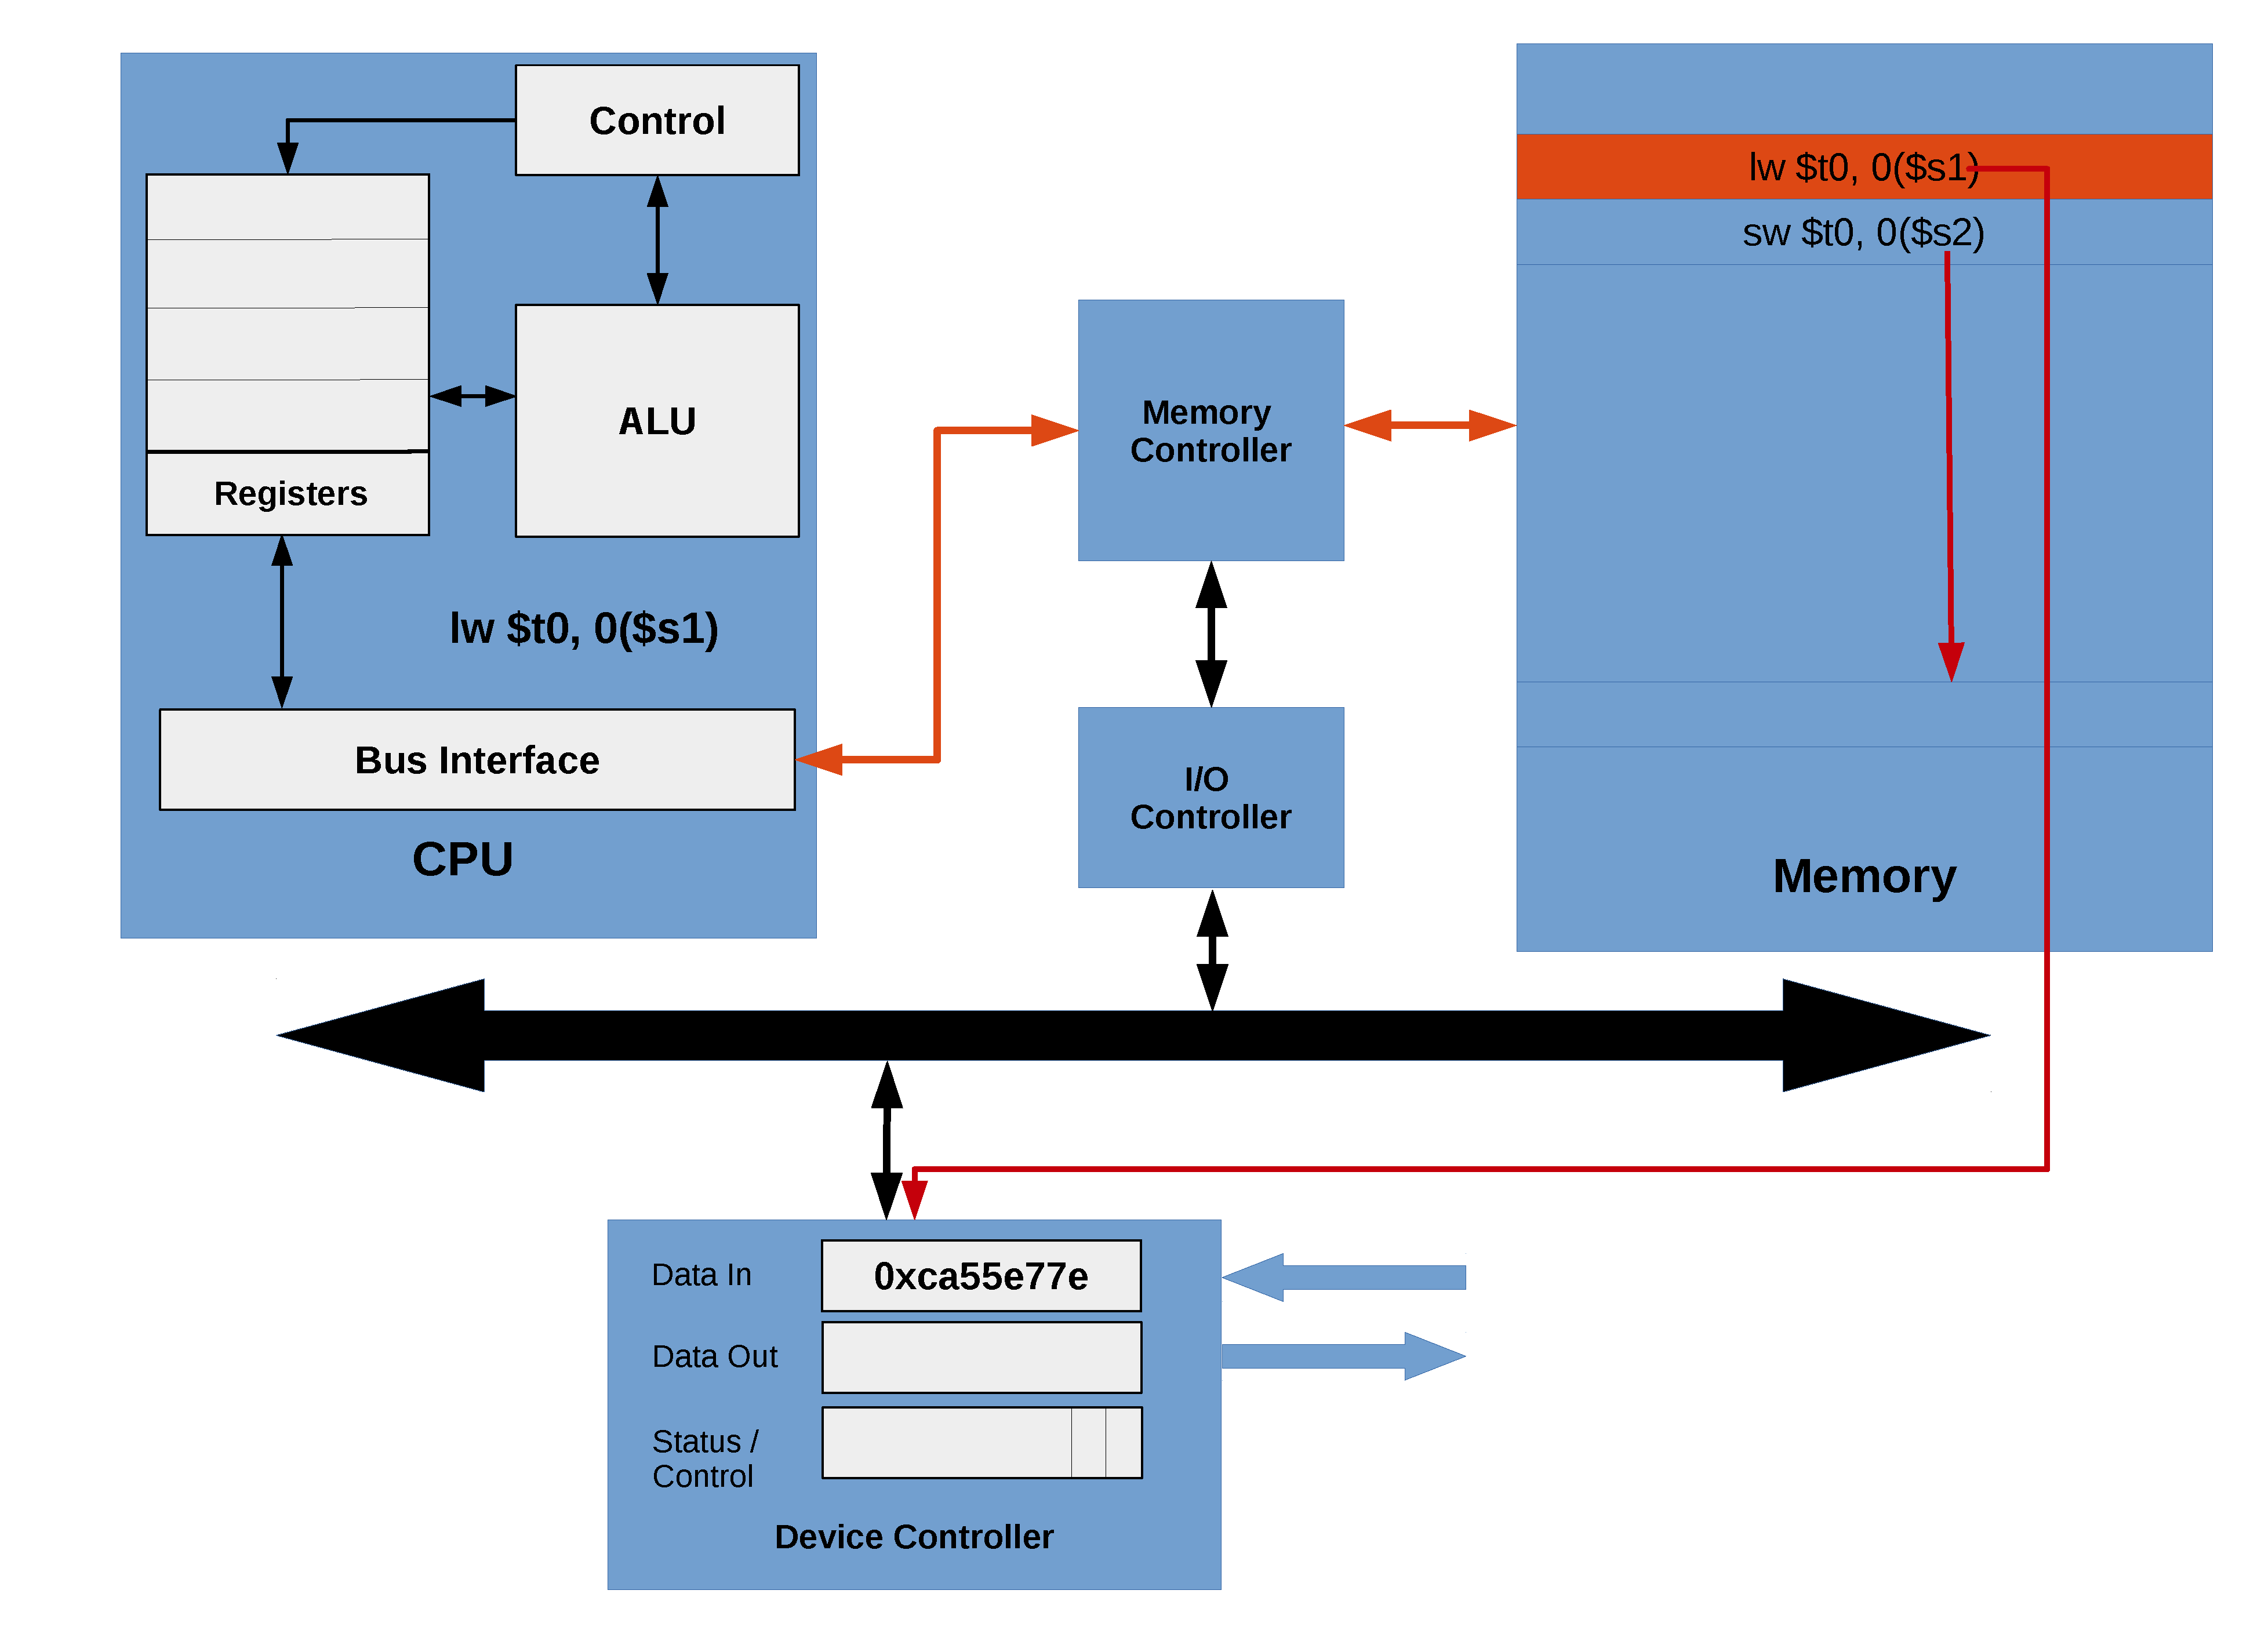
\includegraphics[width=10cm]{io_device3.pdf}
\end{center}

\end{frame}

\begin{frame}%[fragile]
\frametitle{I/O Devices}

\vspace*{-0.2cm}
\begin{center}
\hspace*{-1cm}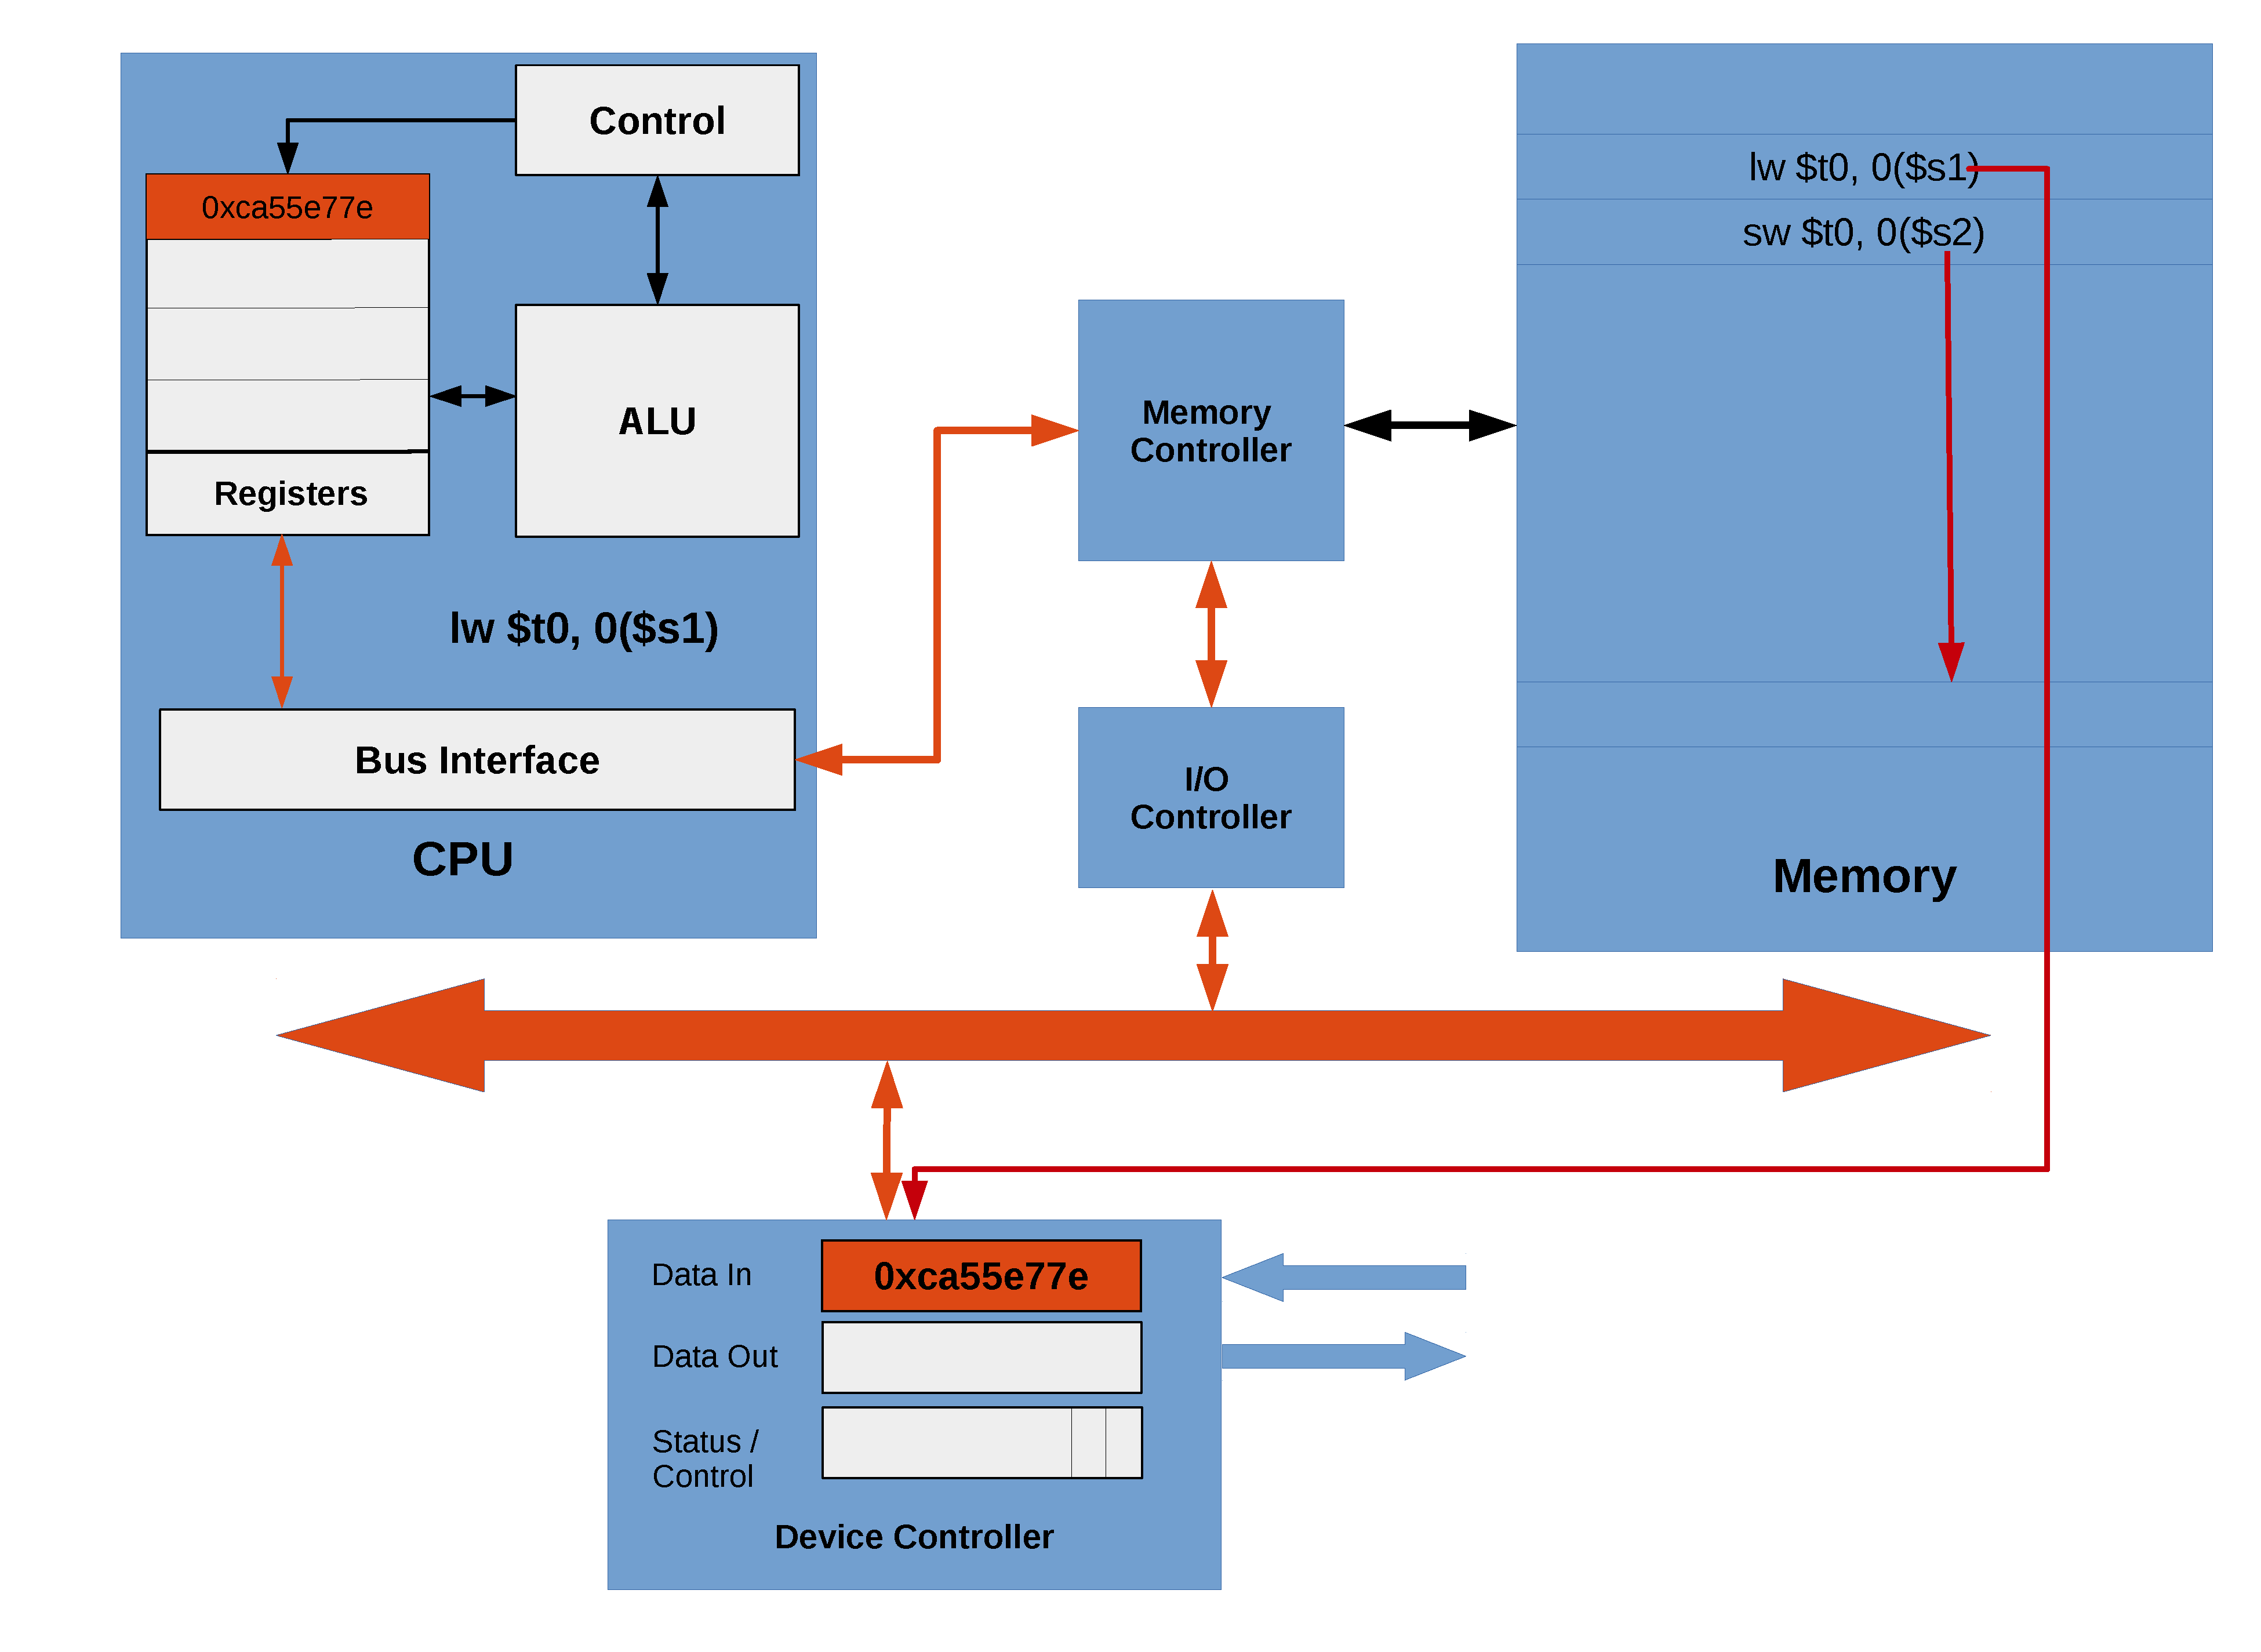
\includegraphics[width=10cm]{io_device4.pdf}
\end{center}

\end{frame}

\begin{frame}%[fragile]
\frametitle{I/O Devices}

\vspace*{-0.2cm}
\begin{center}
\hspace*{-1cm}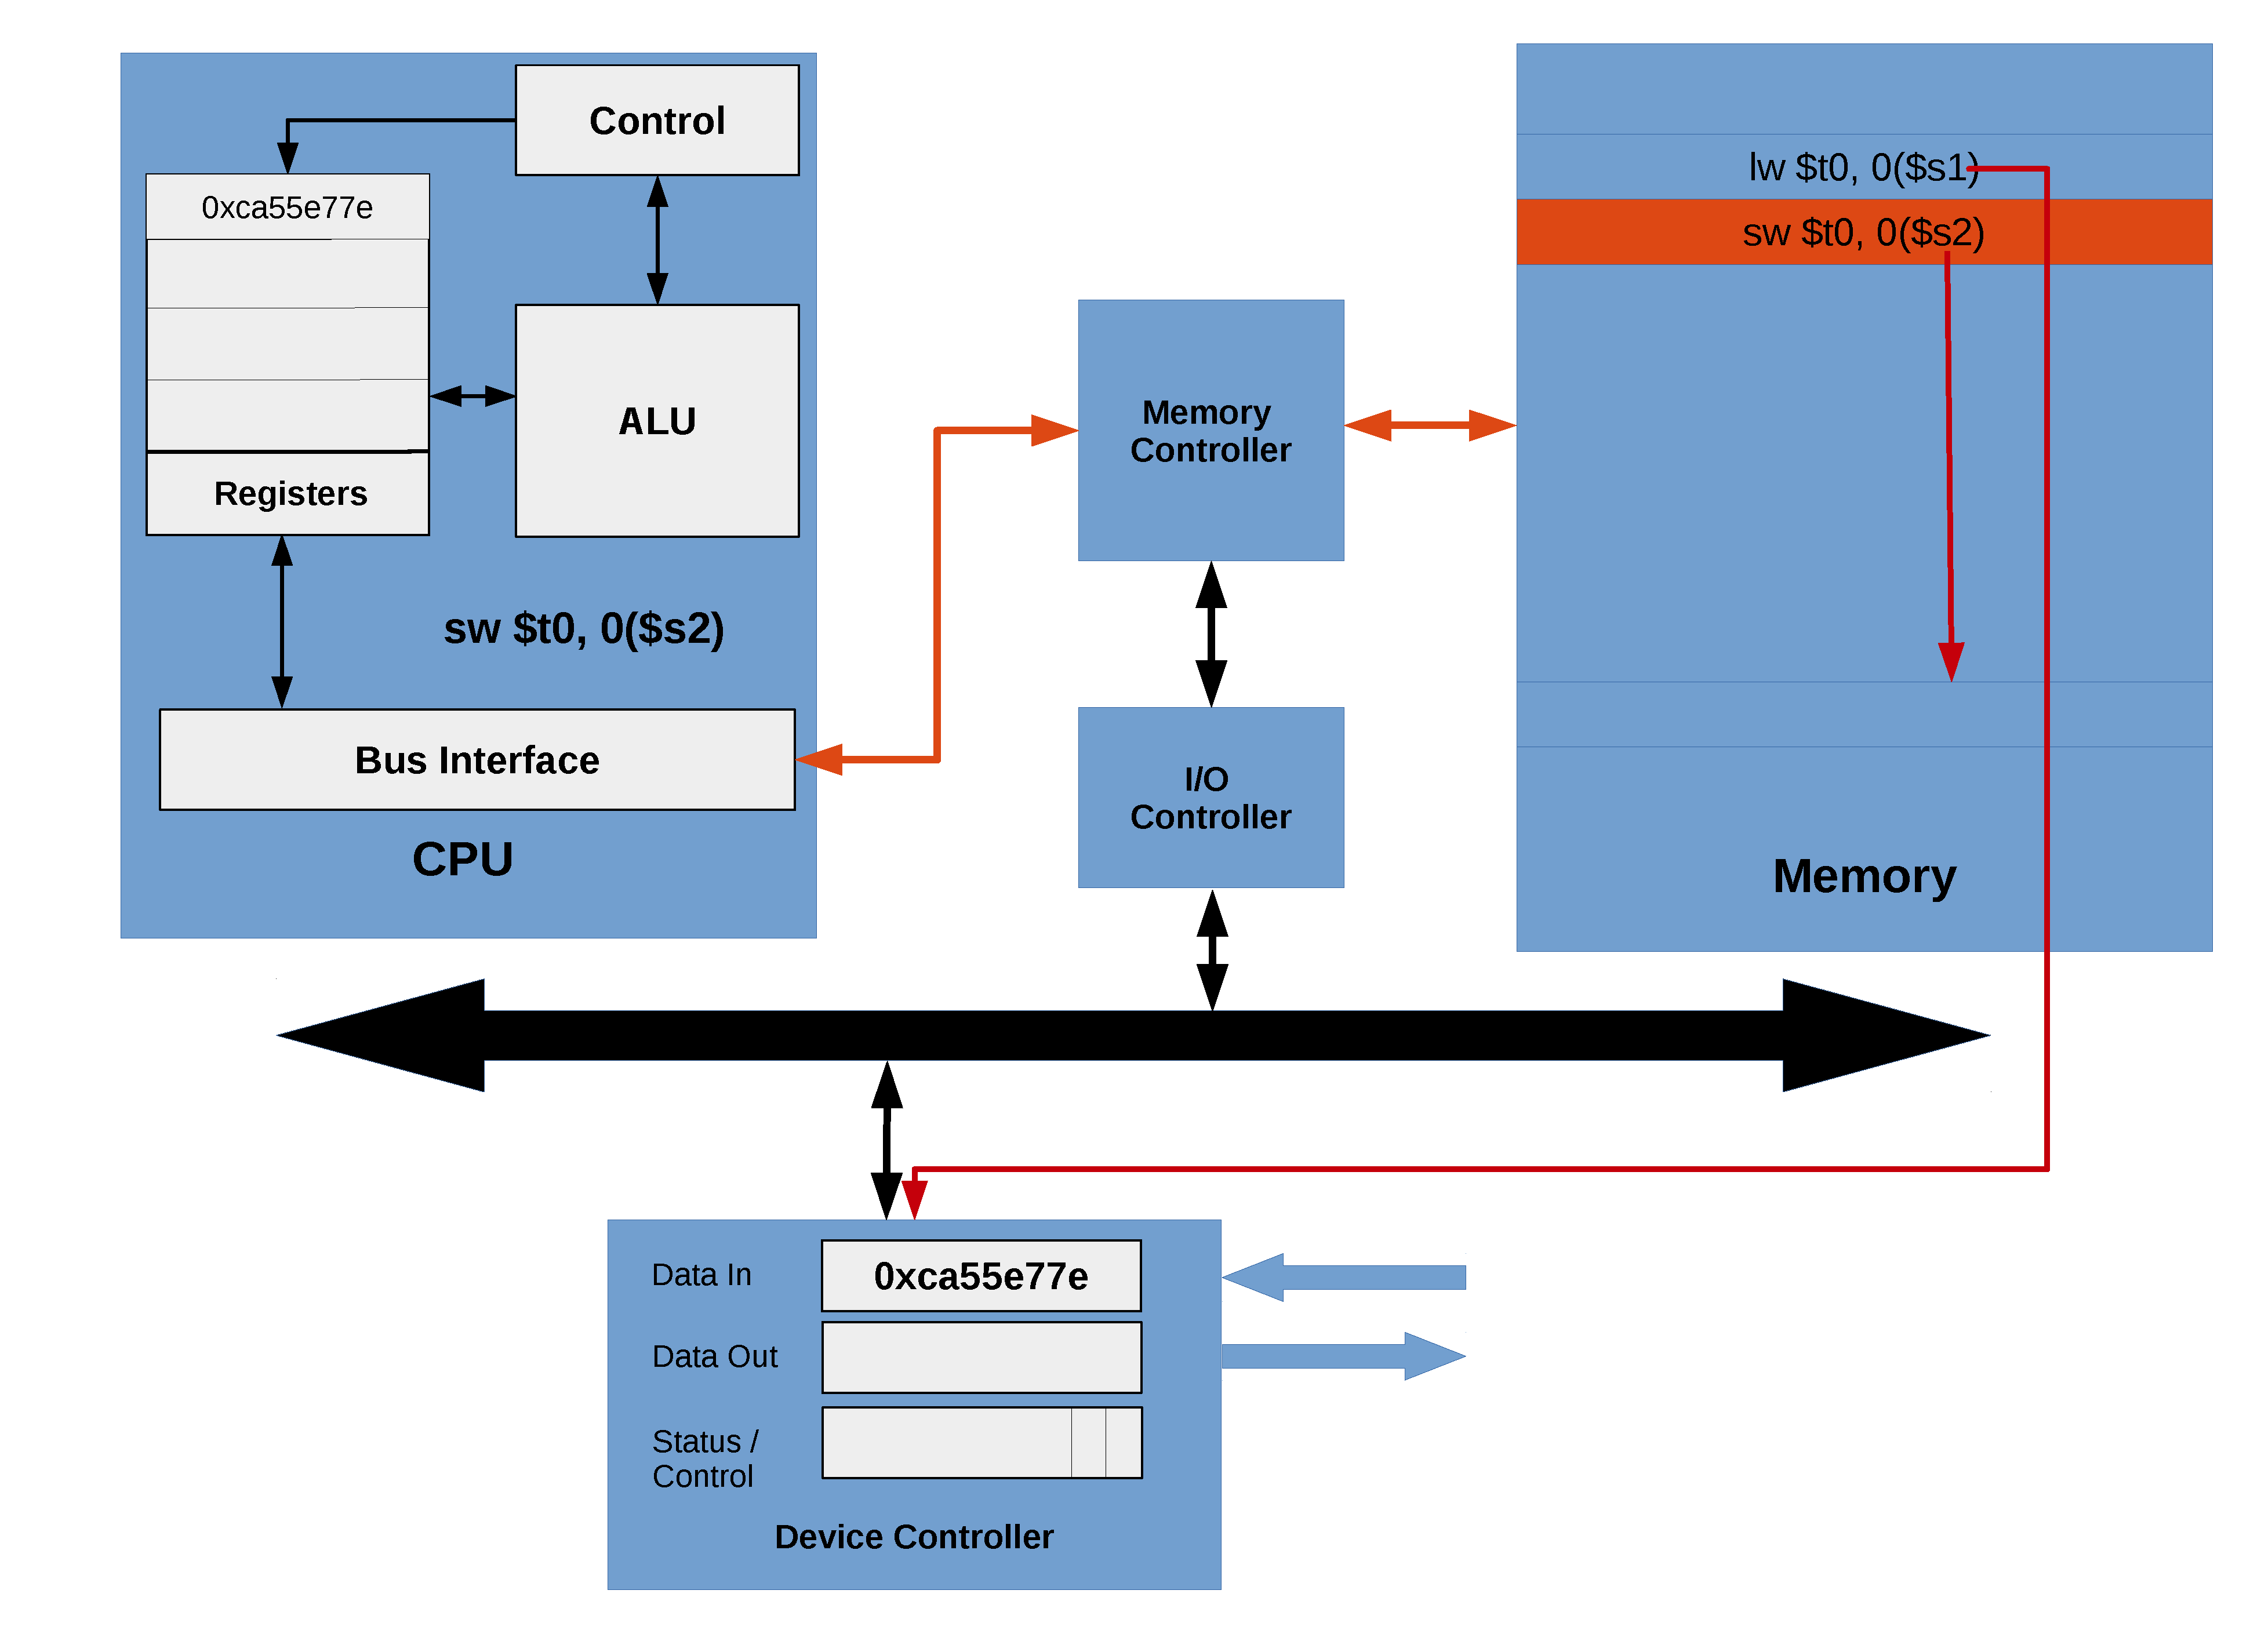
\includegraphics[width=10cm]{io_device5.pdf}
\end{center}

\end{frame}

\begin{frame}%[fragile]
\frametitle{I/O Devices}

\vspace*{-0.2cm}
\begin{center}
\hspace*{-1cm}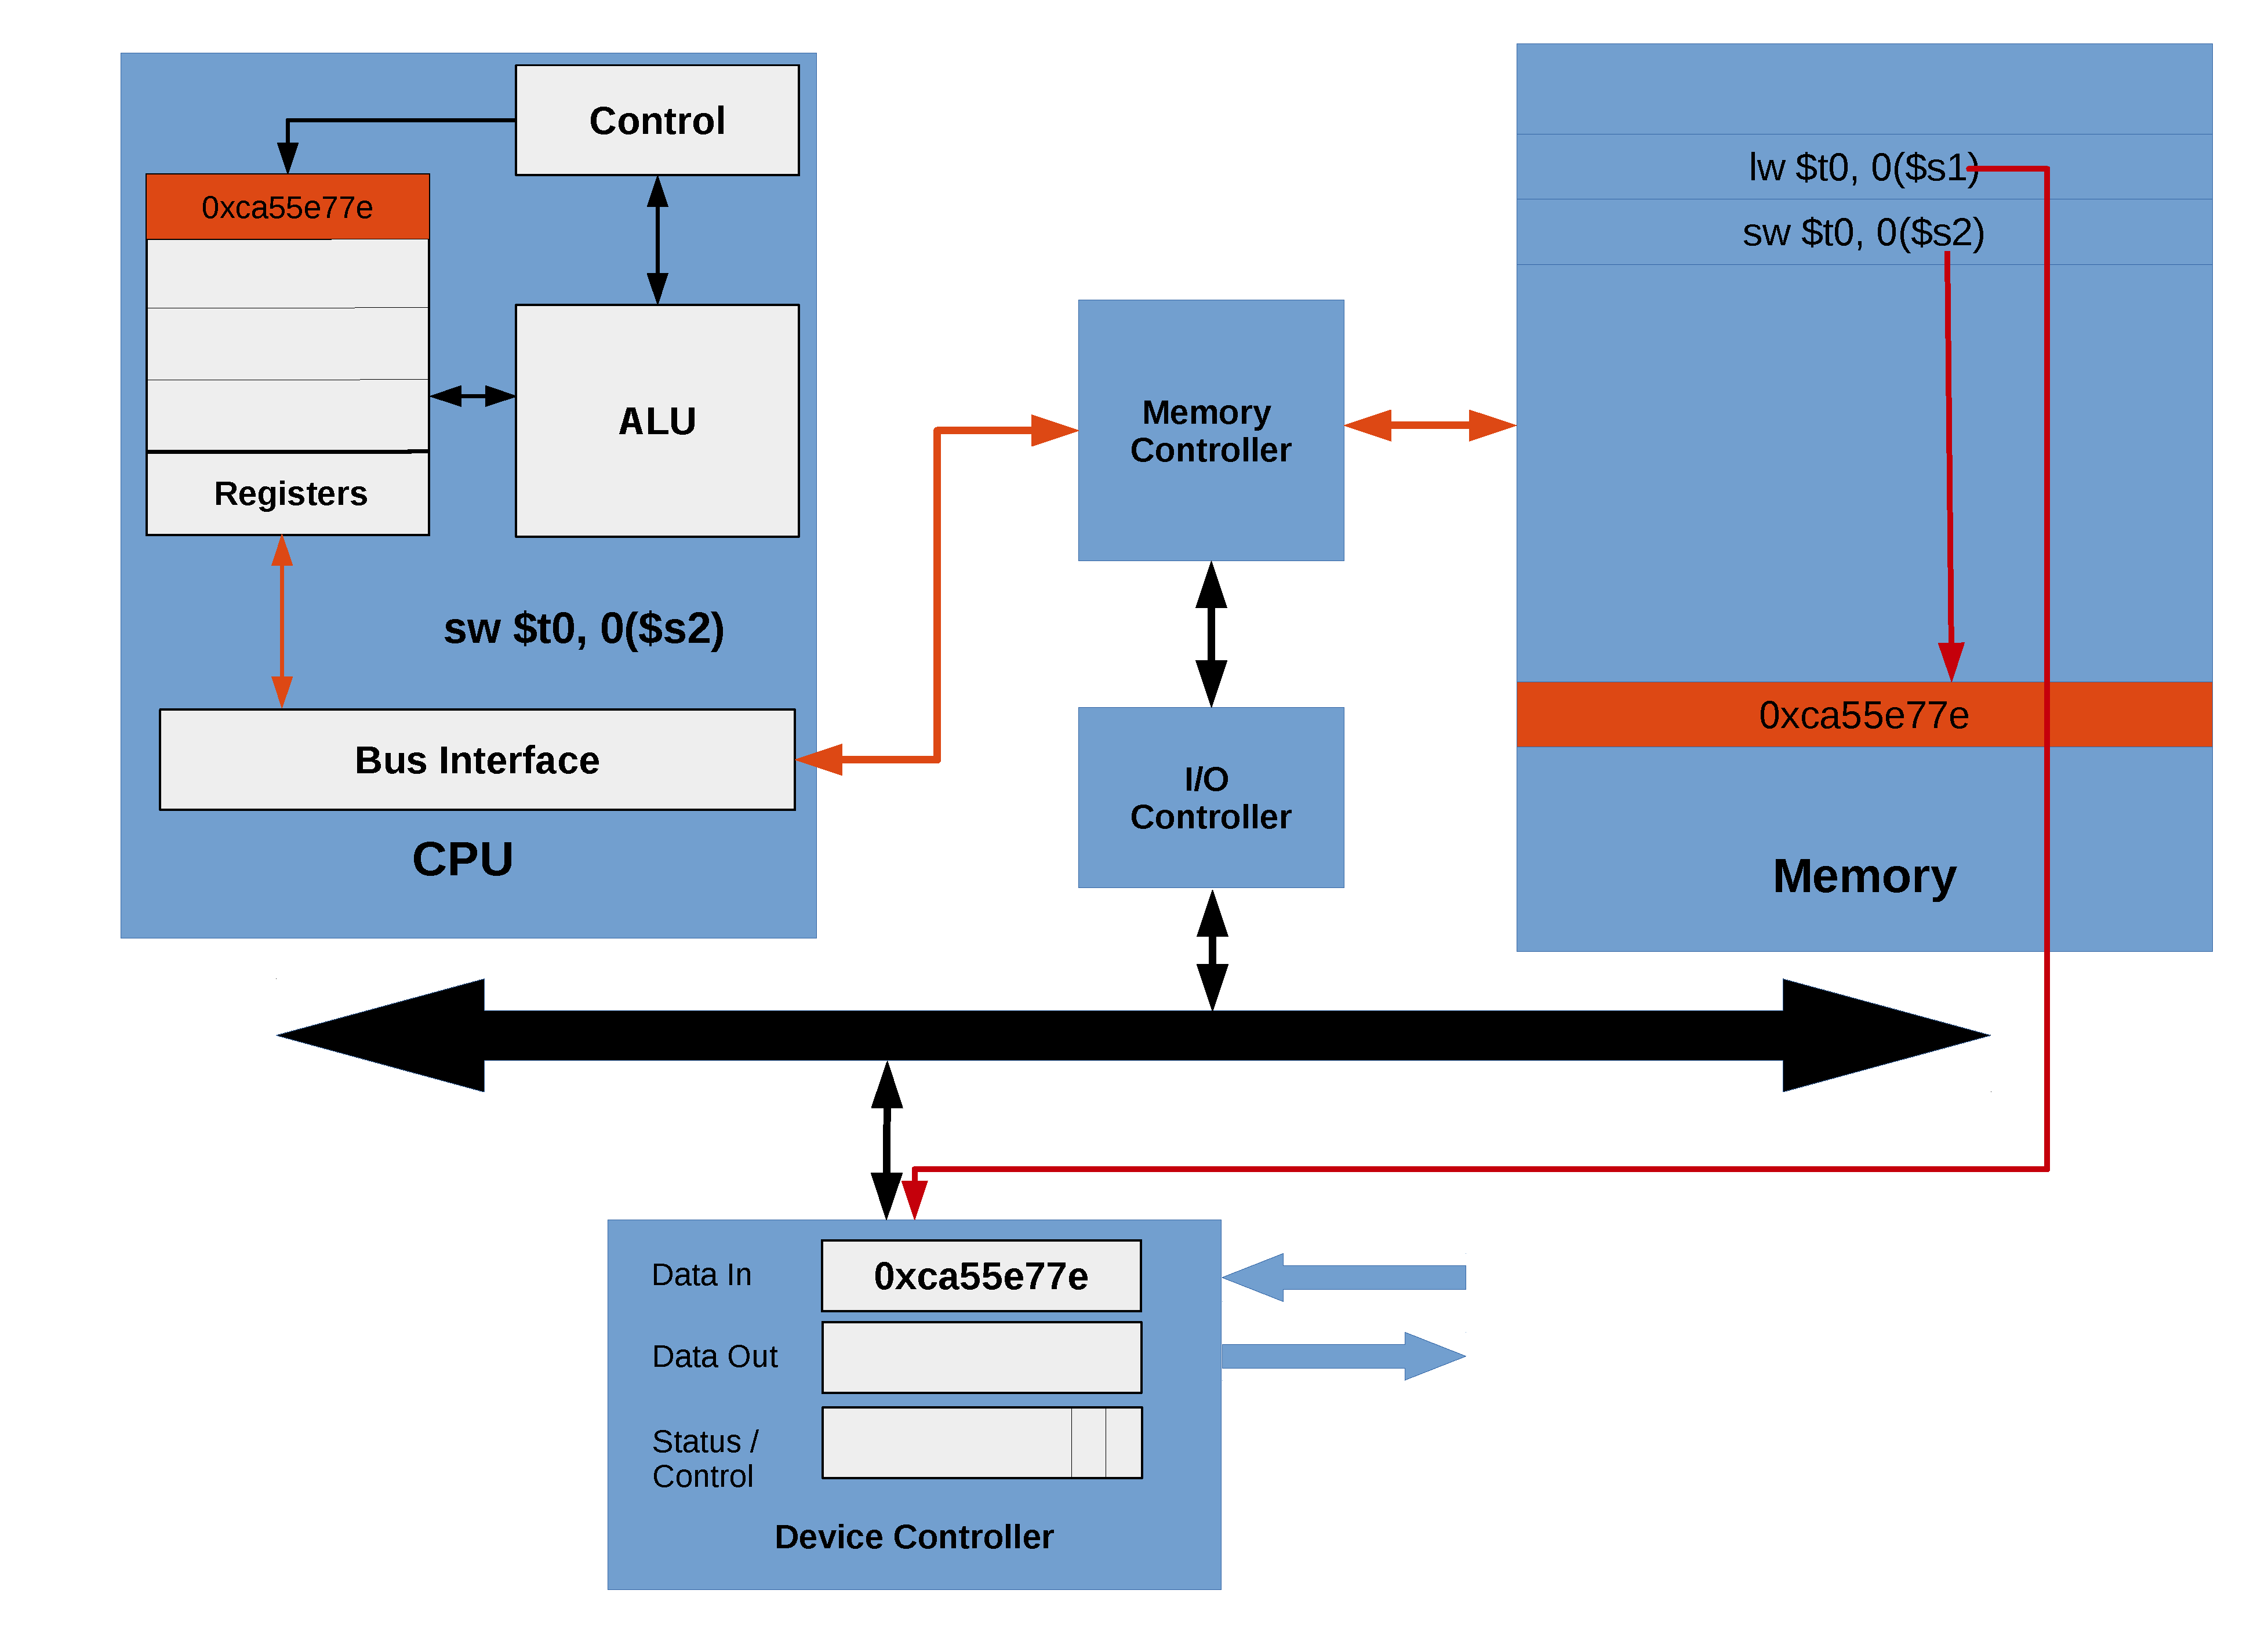
\includegraphics[width=10cm]{io_device6.pdf}
\end{center}

\end{frame}

\subsection{Waiting for I/O Devices}

\begin{frame}%[fragile]
\frametitle{Waiting for I/O Devices}

\end{frame}

\begin{frame}%[fragile]
\frametitle{Busy Waiting}

\vspace*{-0.2cm}
\begin{center}
\hspace*{-1cm}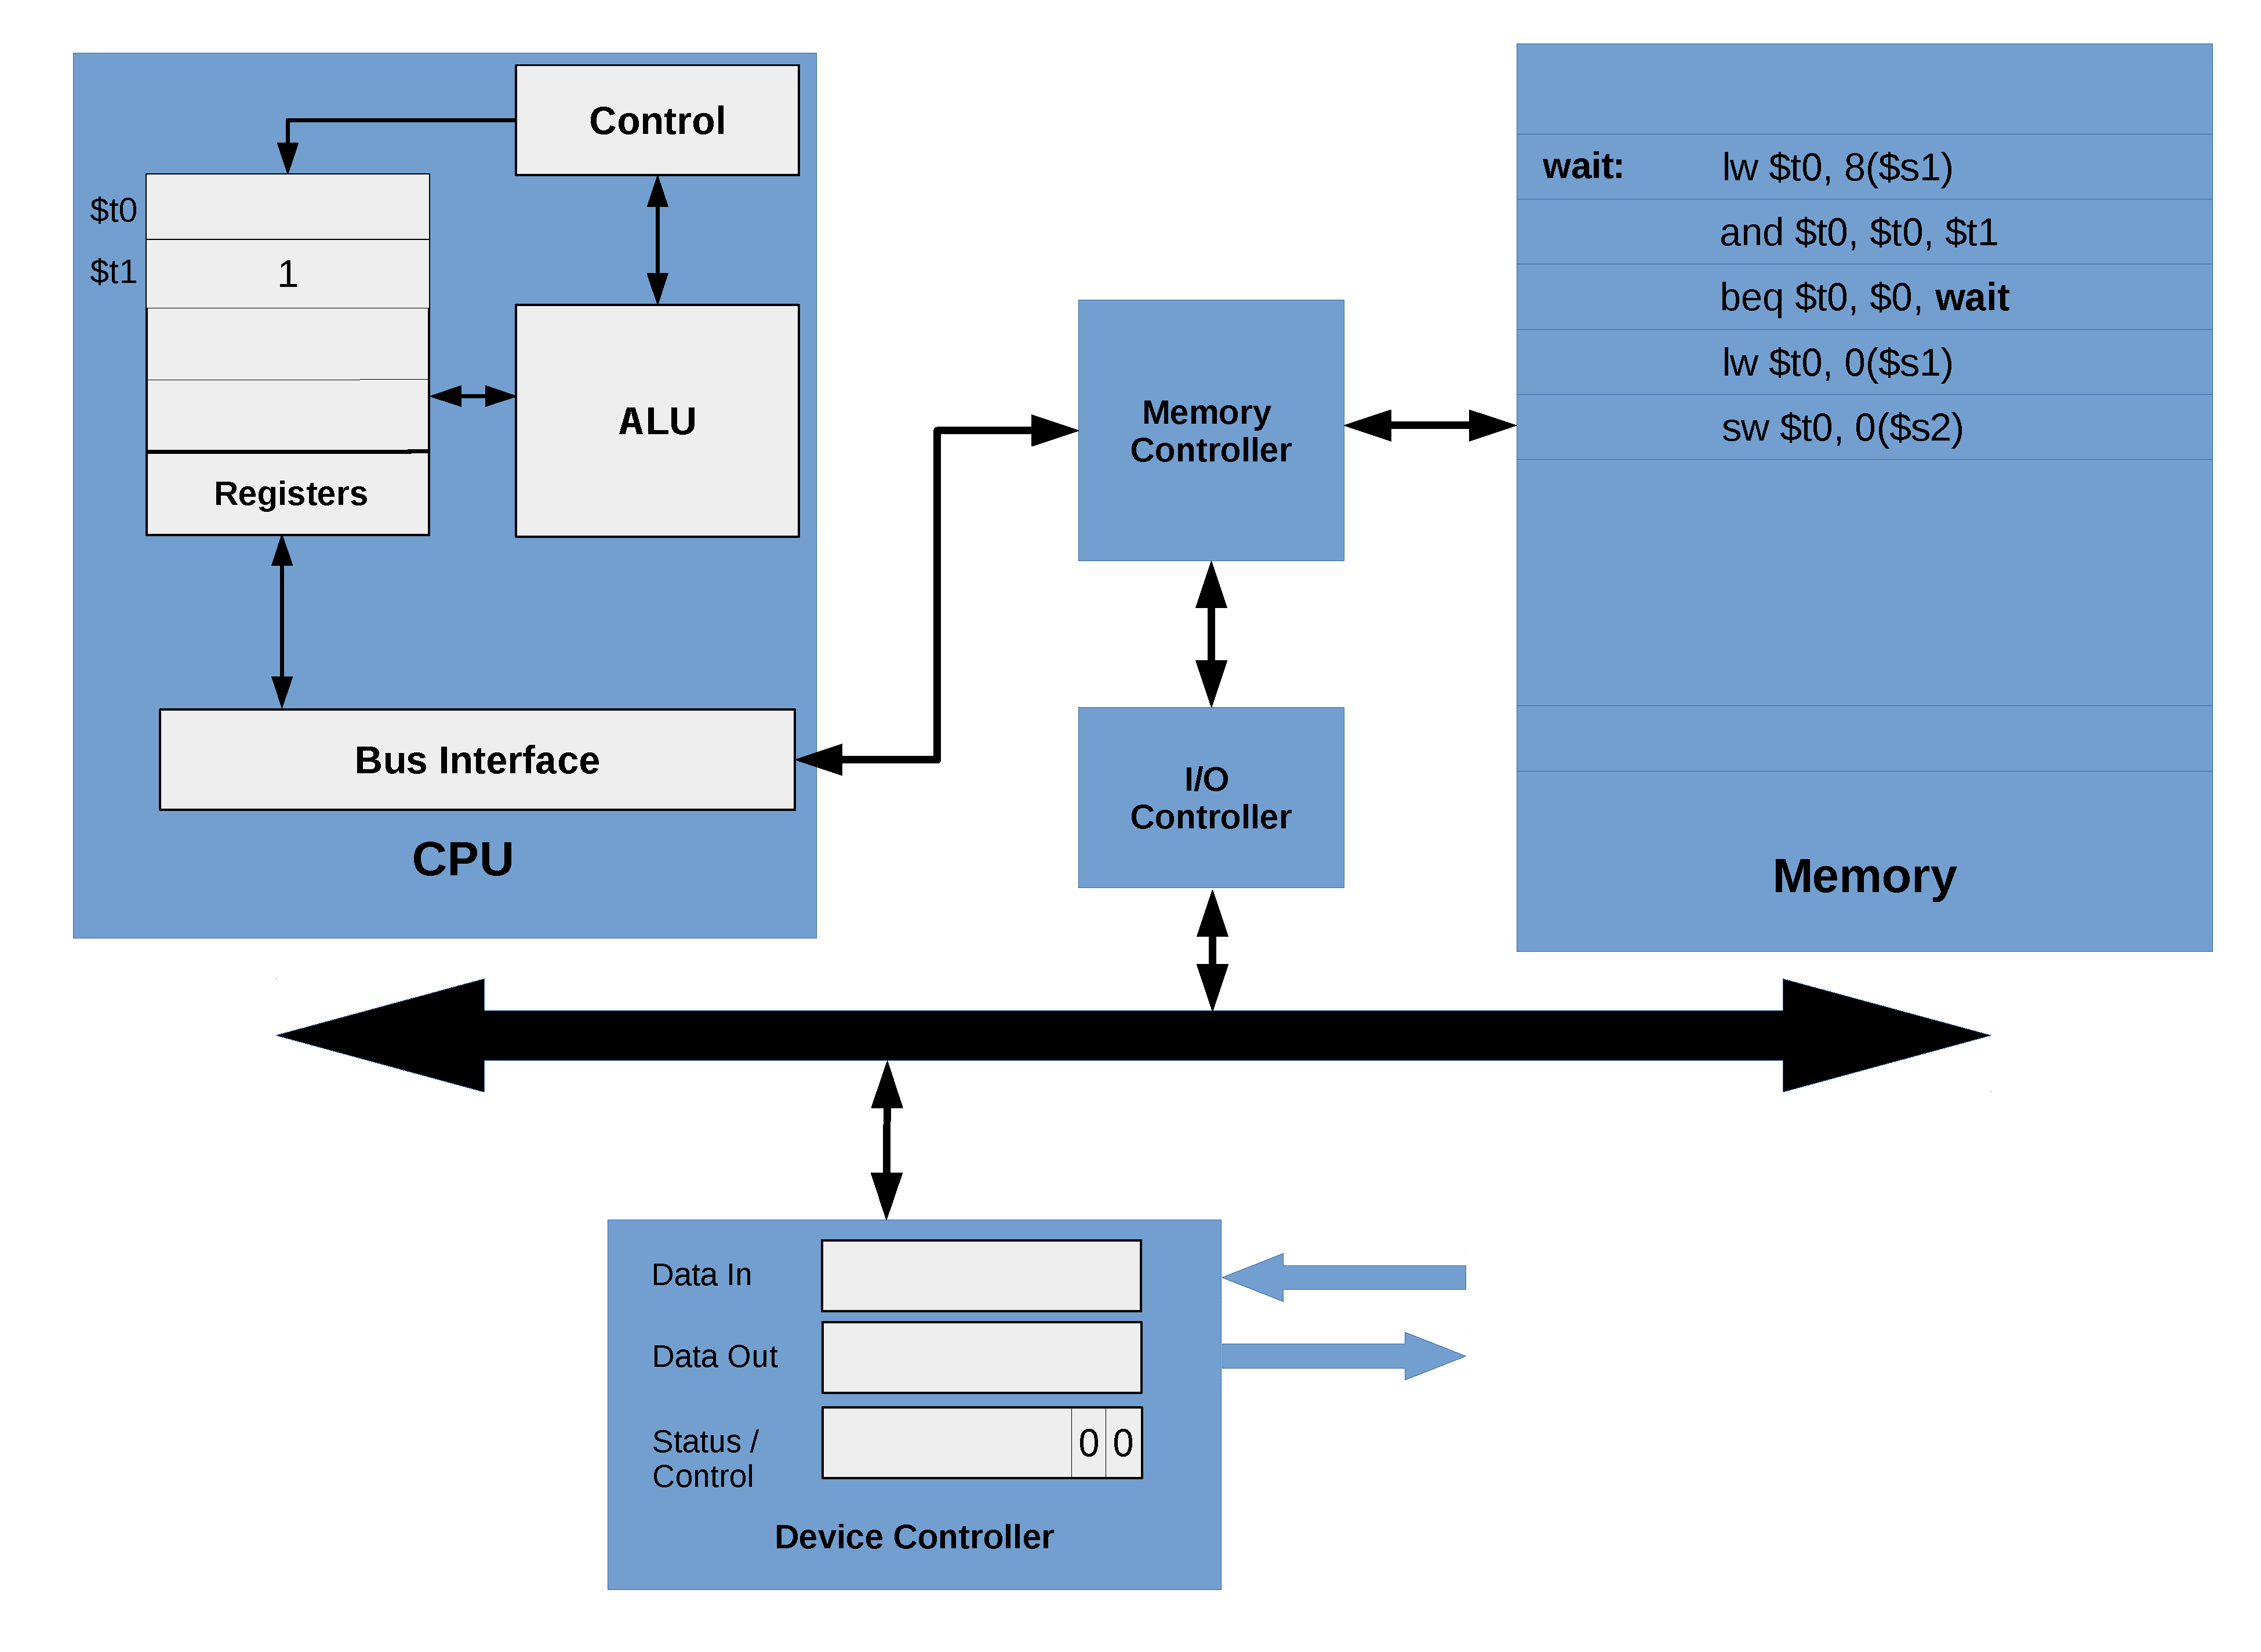
\includegraphics[width=10cm]{busy_waiting1.pdf}
\end{center}

\end{frame}

\begin{frame}%[fragile]
\frametitle{Busy Waiting}

\vspace*{-0.2cm}
\begin{center}
\hspace*{-1cm}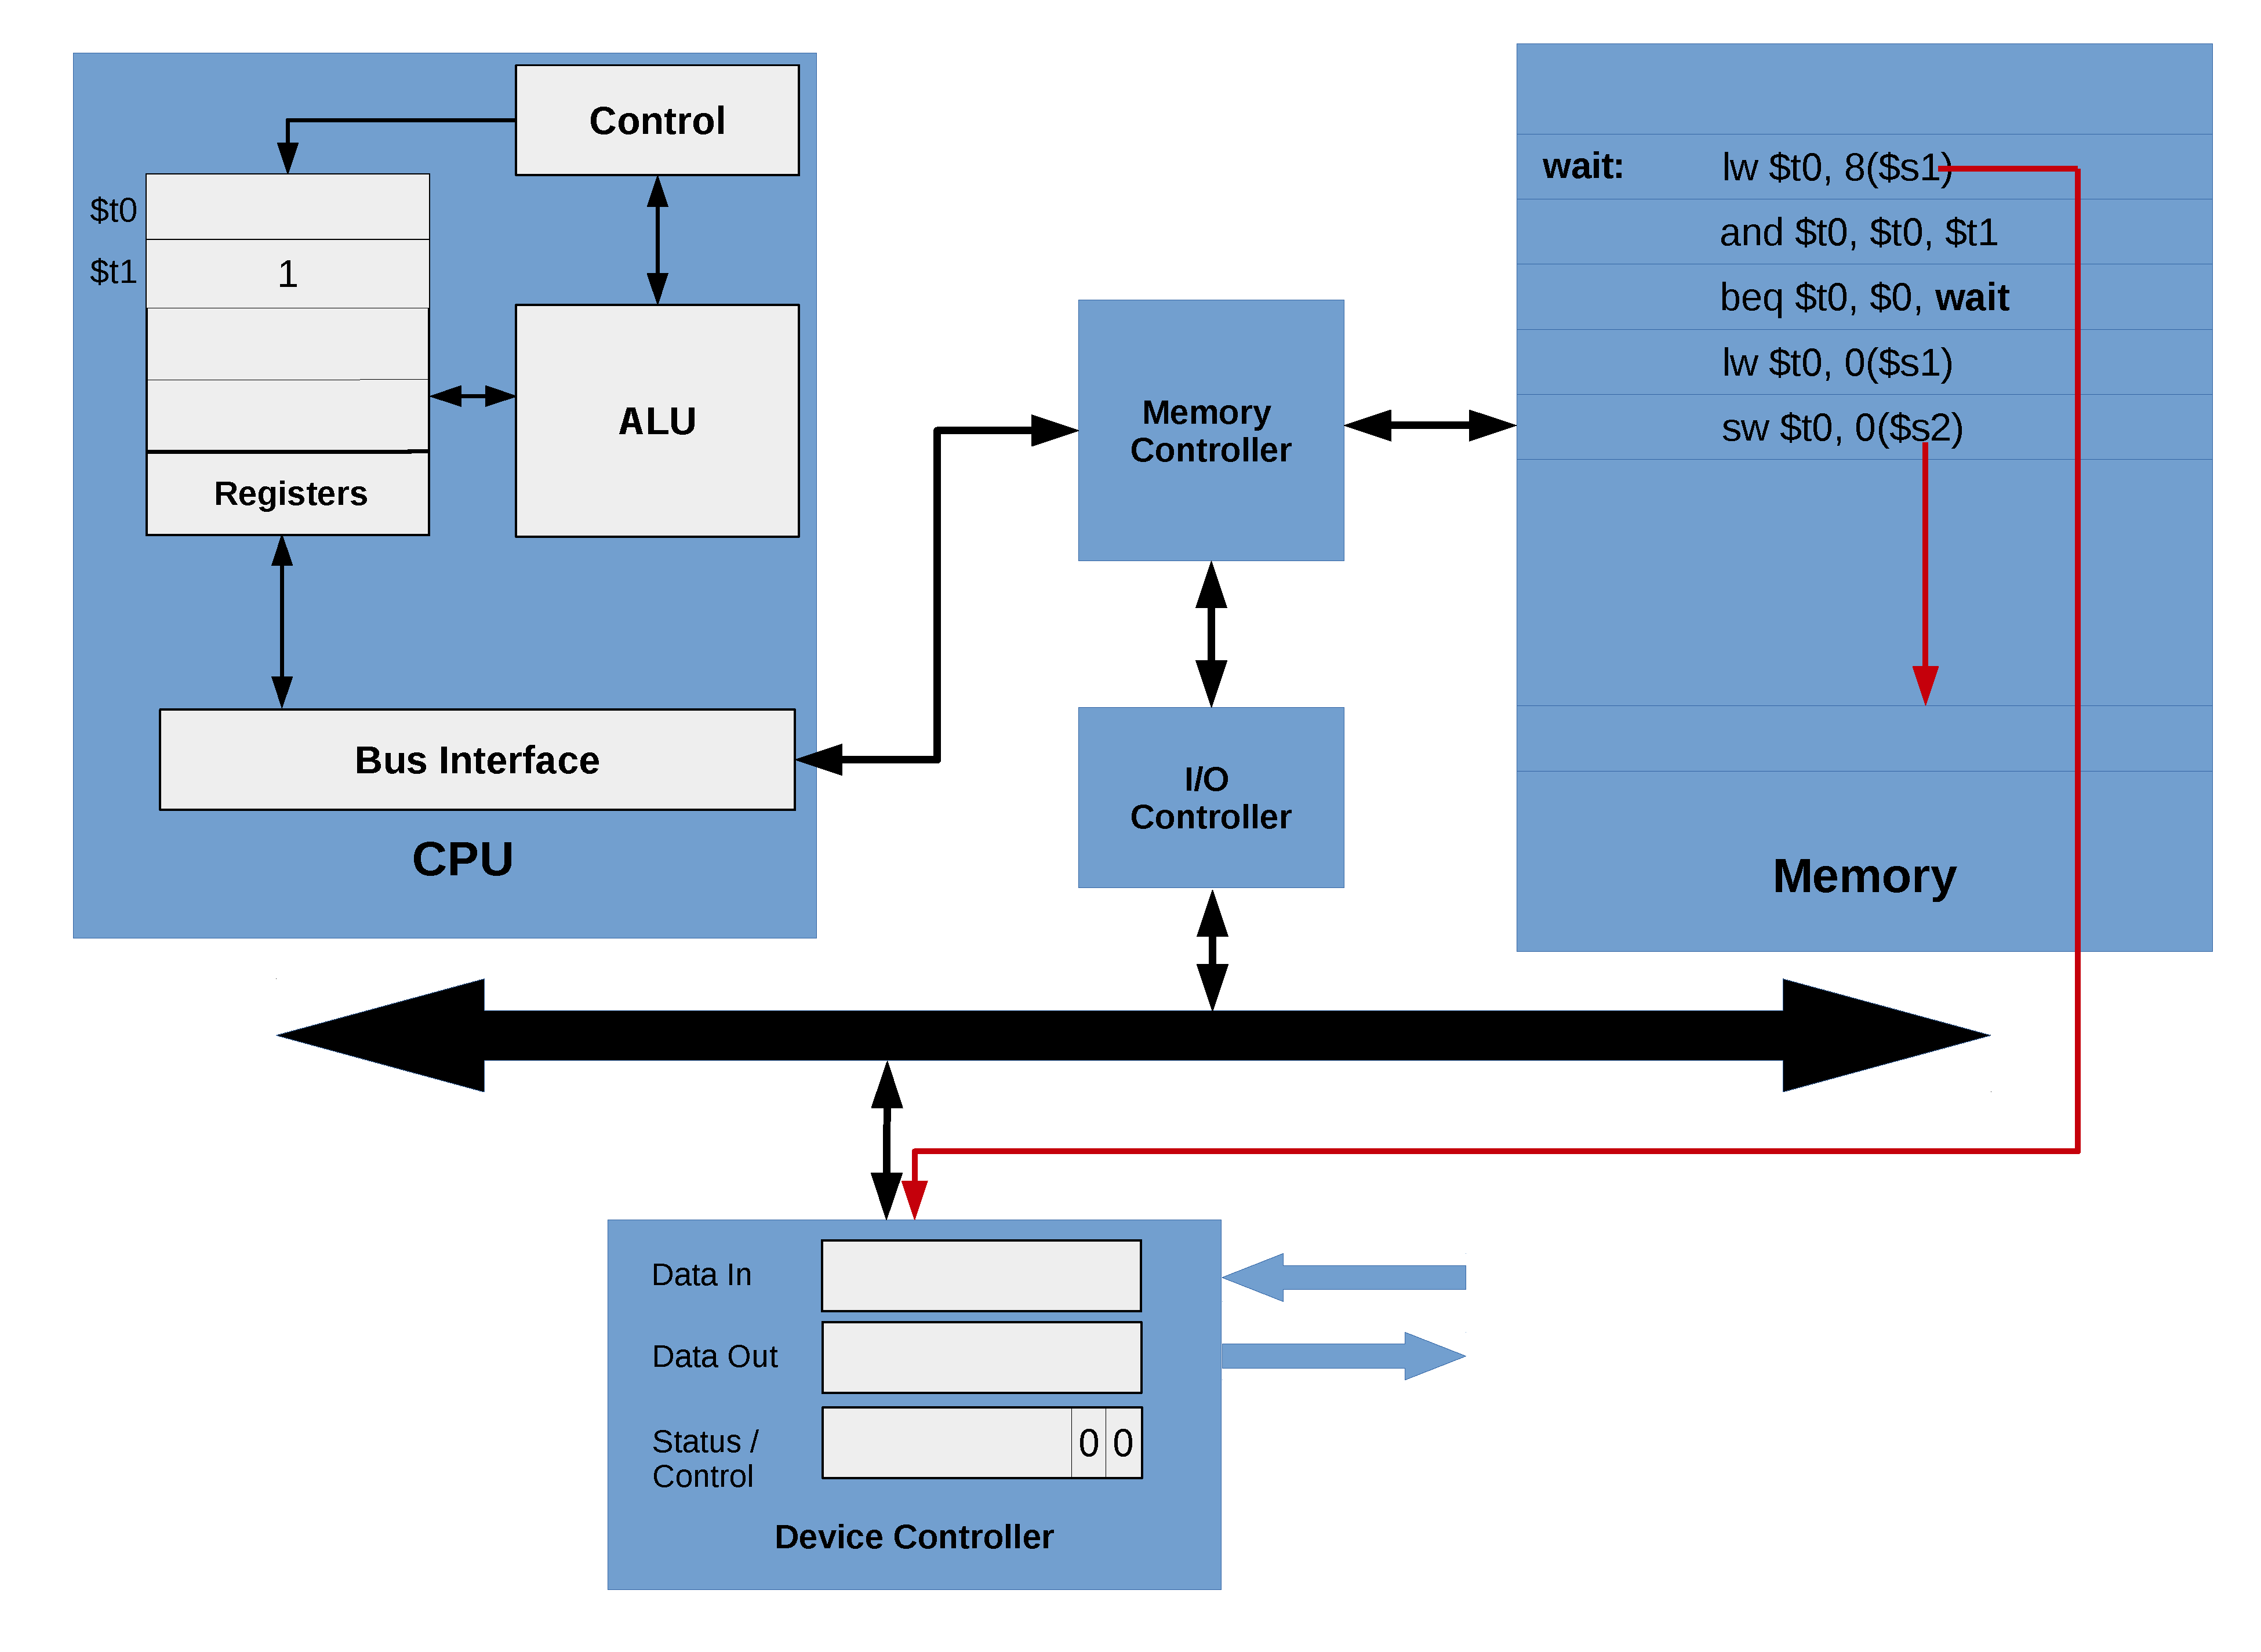
\includegraphics[width=10cm]{busy_waiting2.pdf}
\end{center}

\end{frame}

\begin{frame}%[fragile]
\frametitle{Busy Waiting}

\vspace*{-0.2cm}
\begin{center}
\hspace*{-1cm}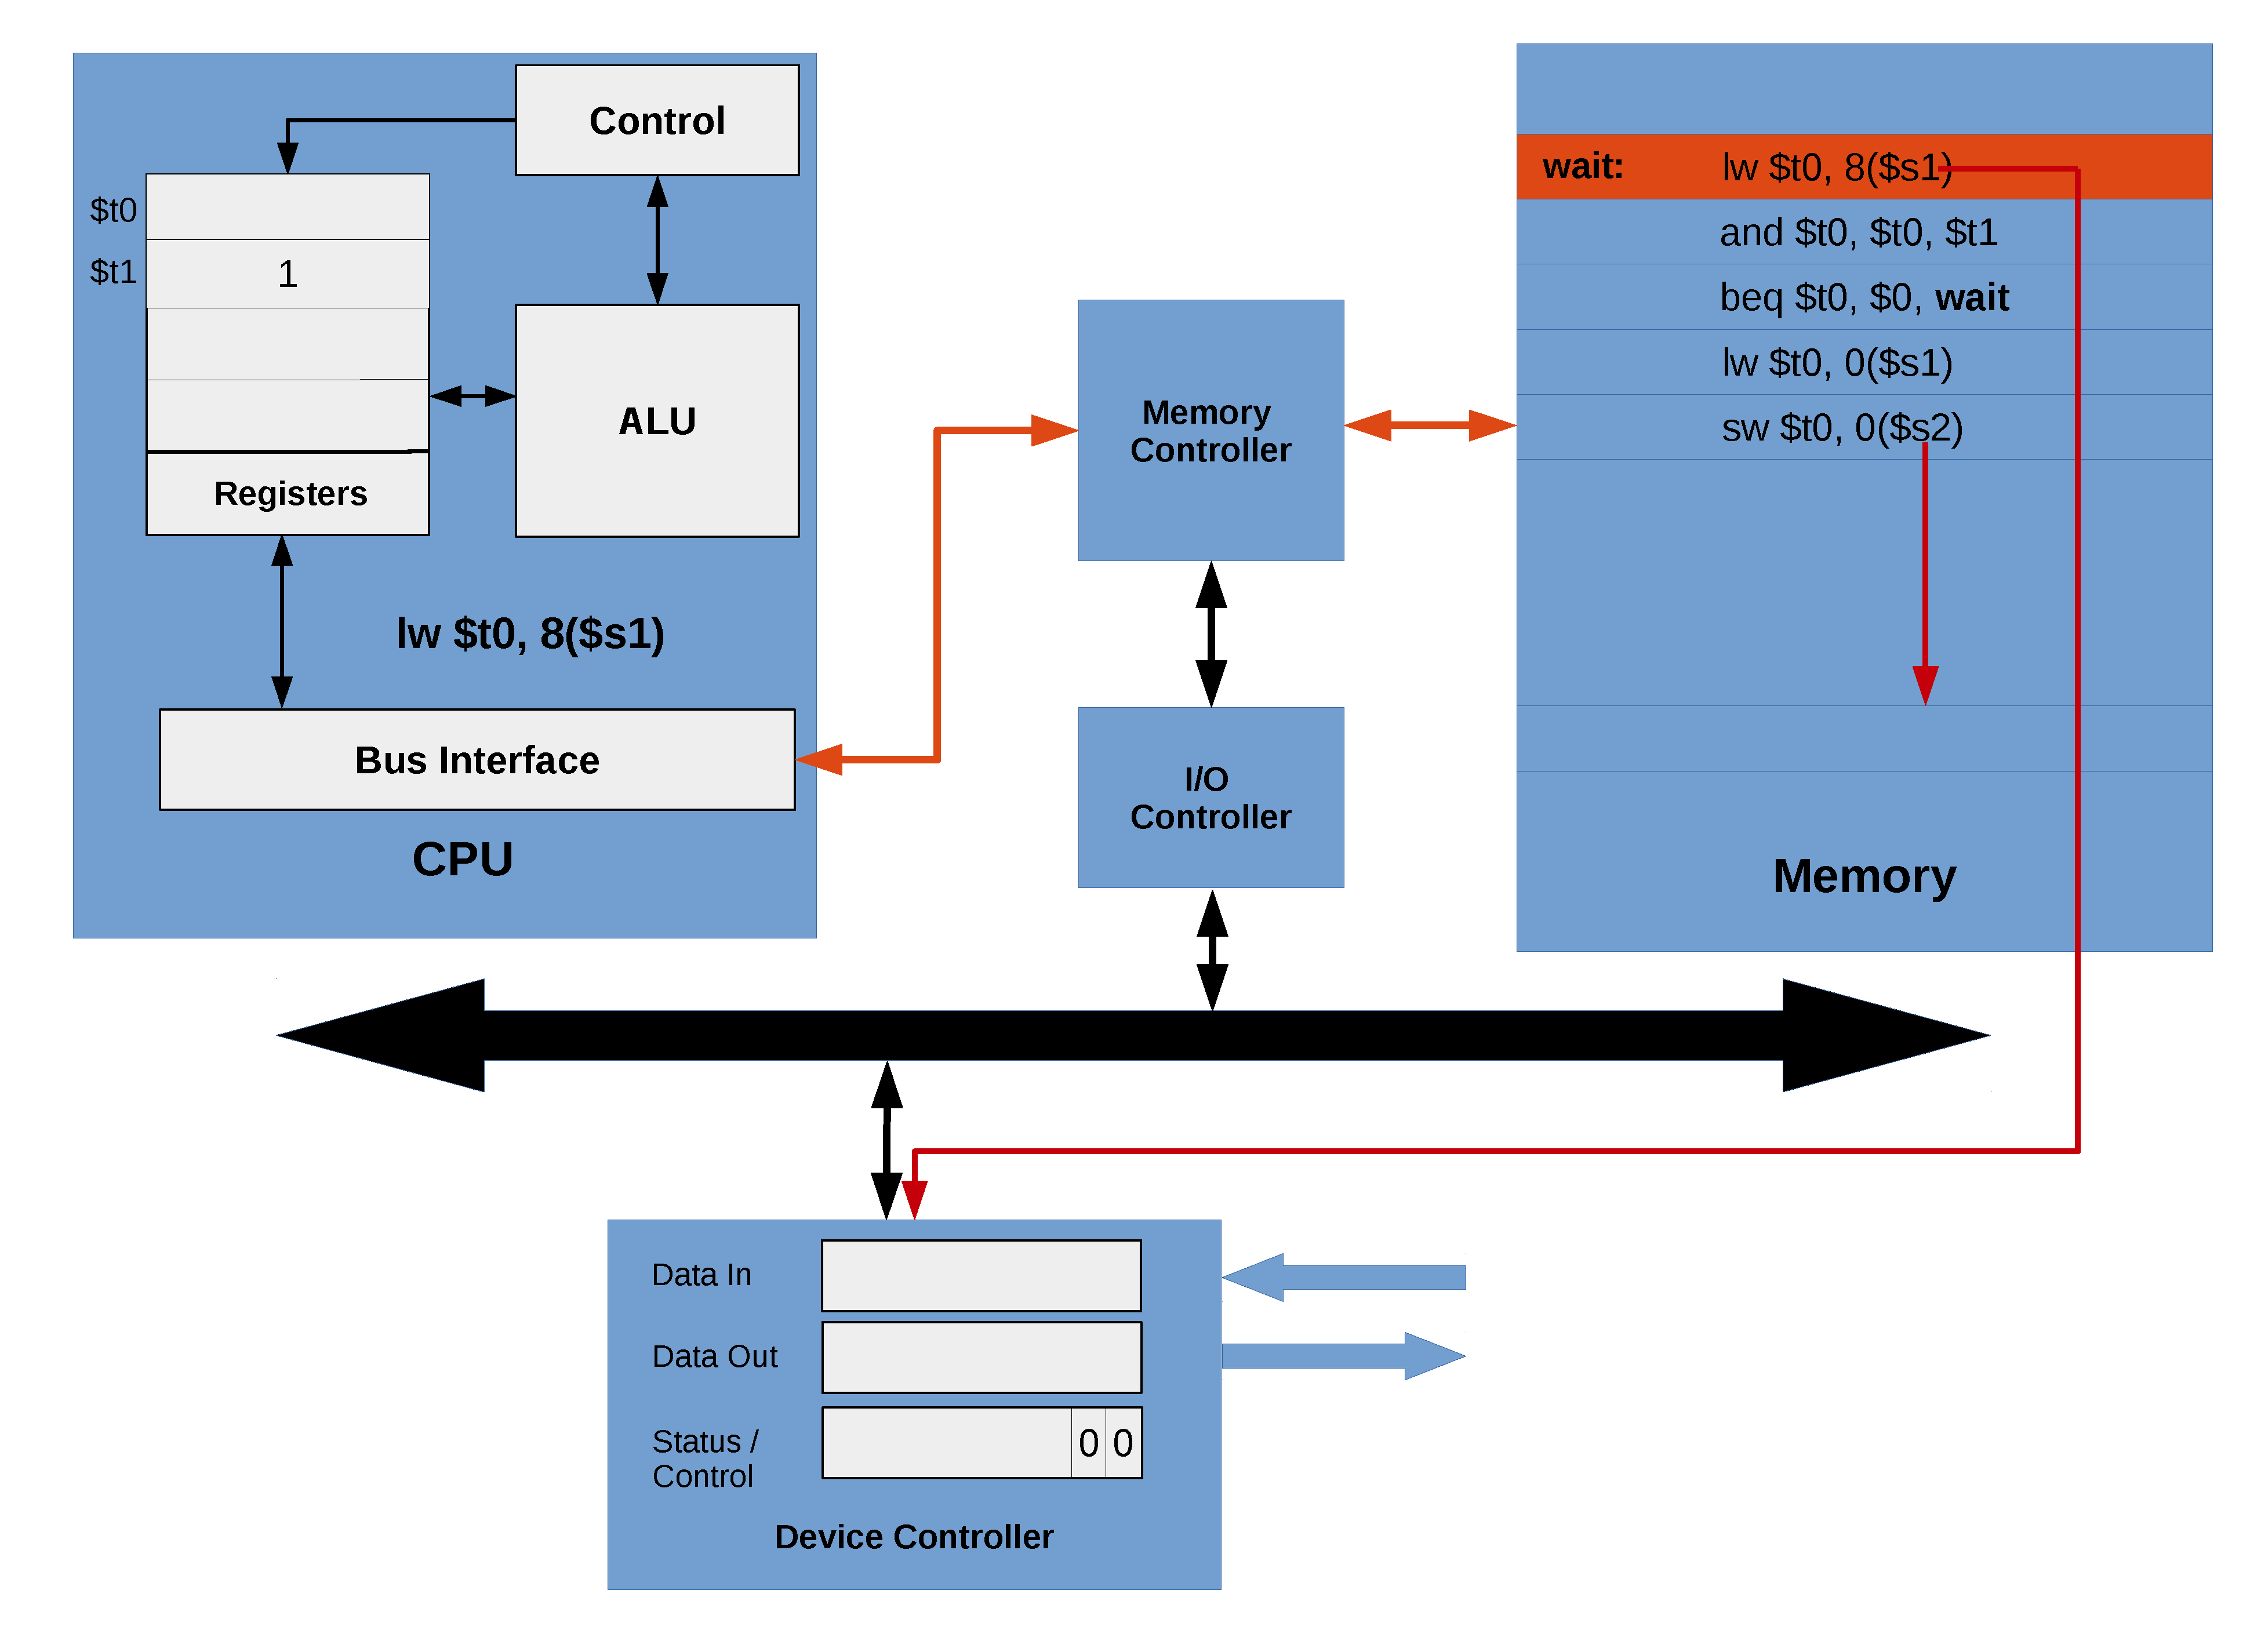
\includegraphics[width=10cm]{busy_waiting3.pdf}
\end{center}

\end{frame}

\begin{frame}%[fragile]
\frametitle{Busy Waiting}

\vspace*{-0.2cm}
\begin{center}
\hspace*{-1cm}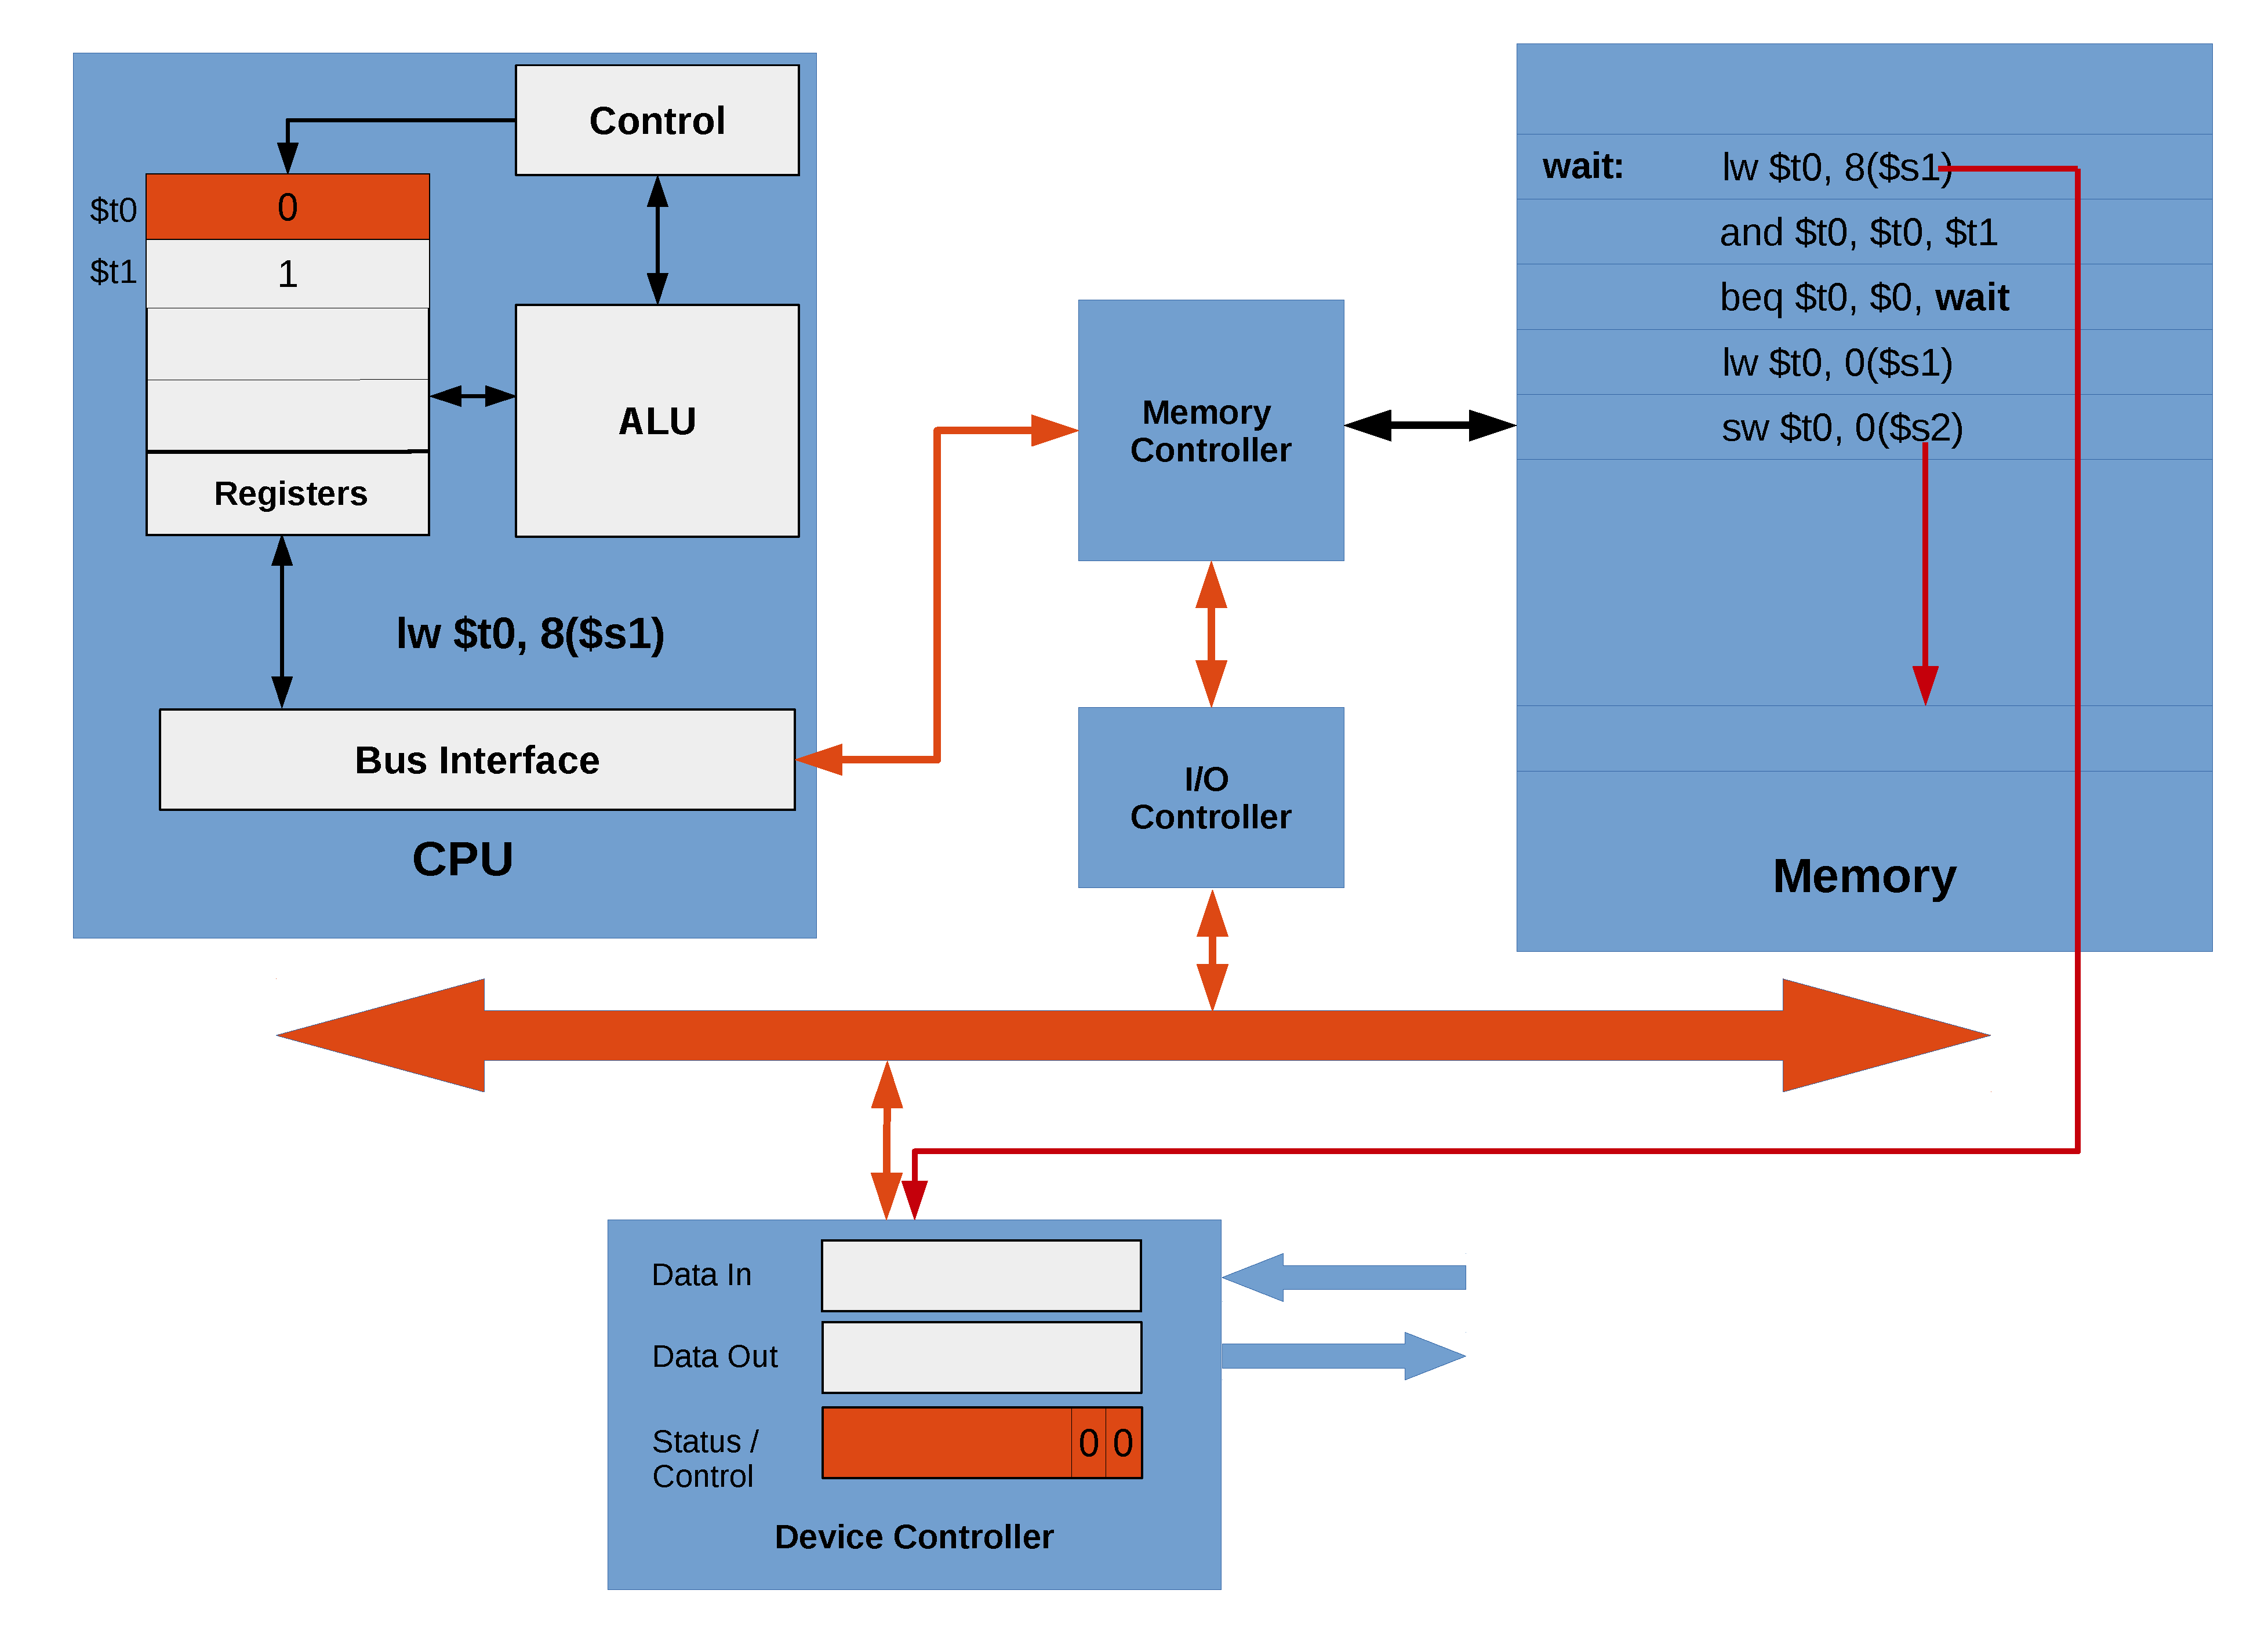
\includegraphics[width=10cm]{busy_waiting4.pdf}
\end{center}

\end{frame}

\begin{frame}%[fragile]
\frametitle{Busy Waiting}

\vspace*{-0.2cm}
\begin{center}
\hspace*{-1cm}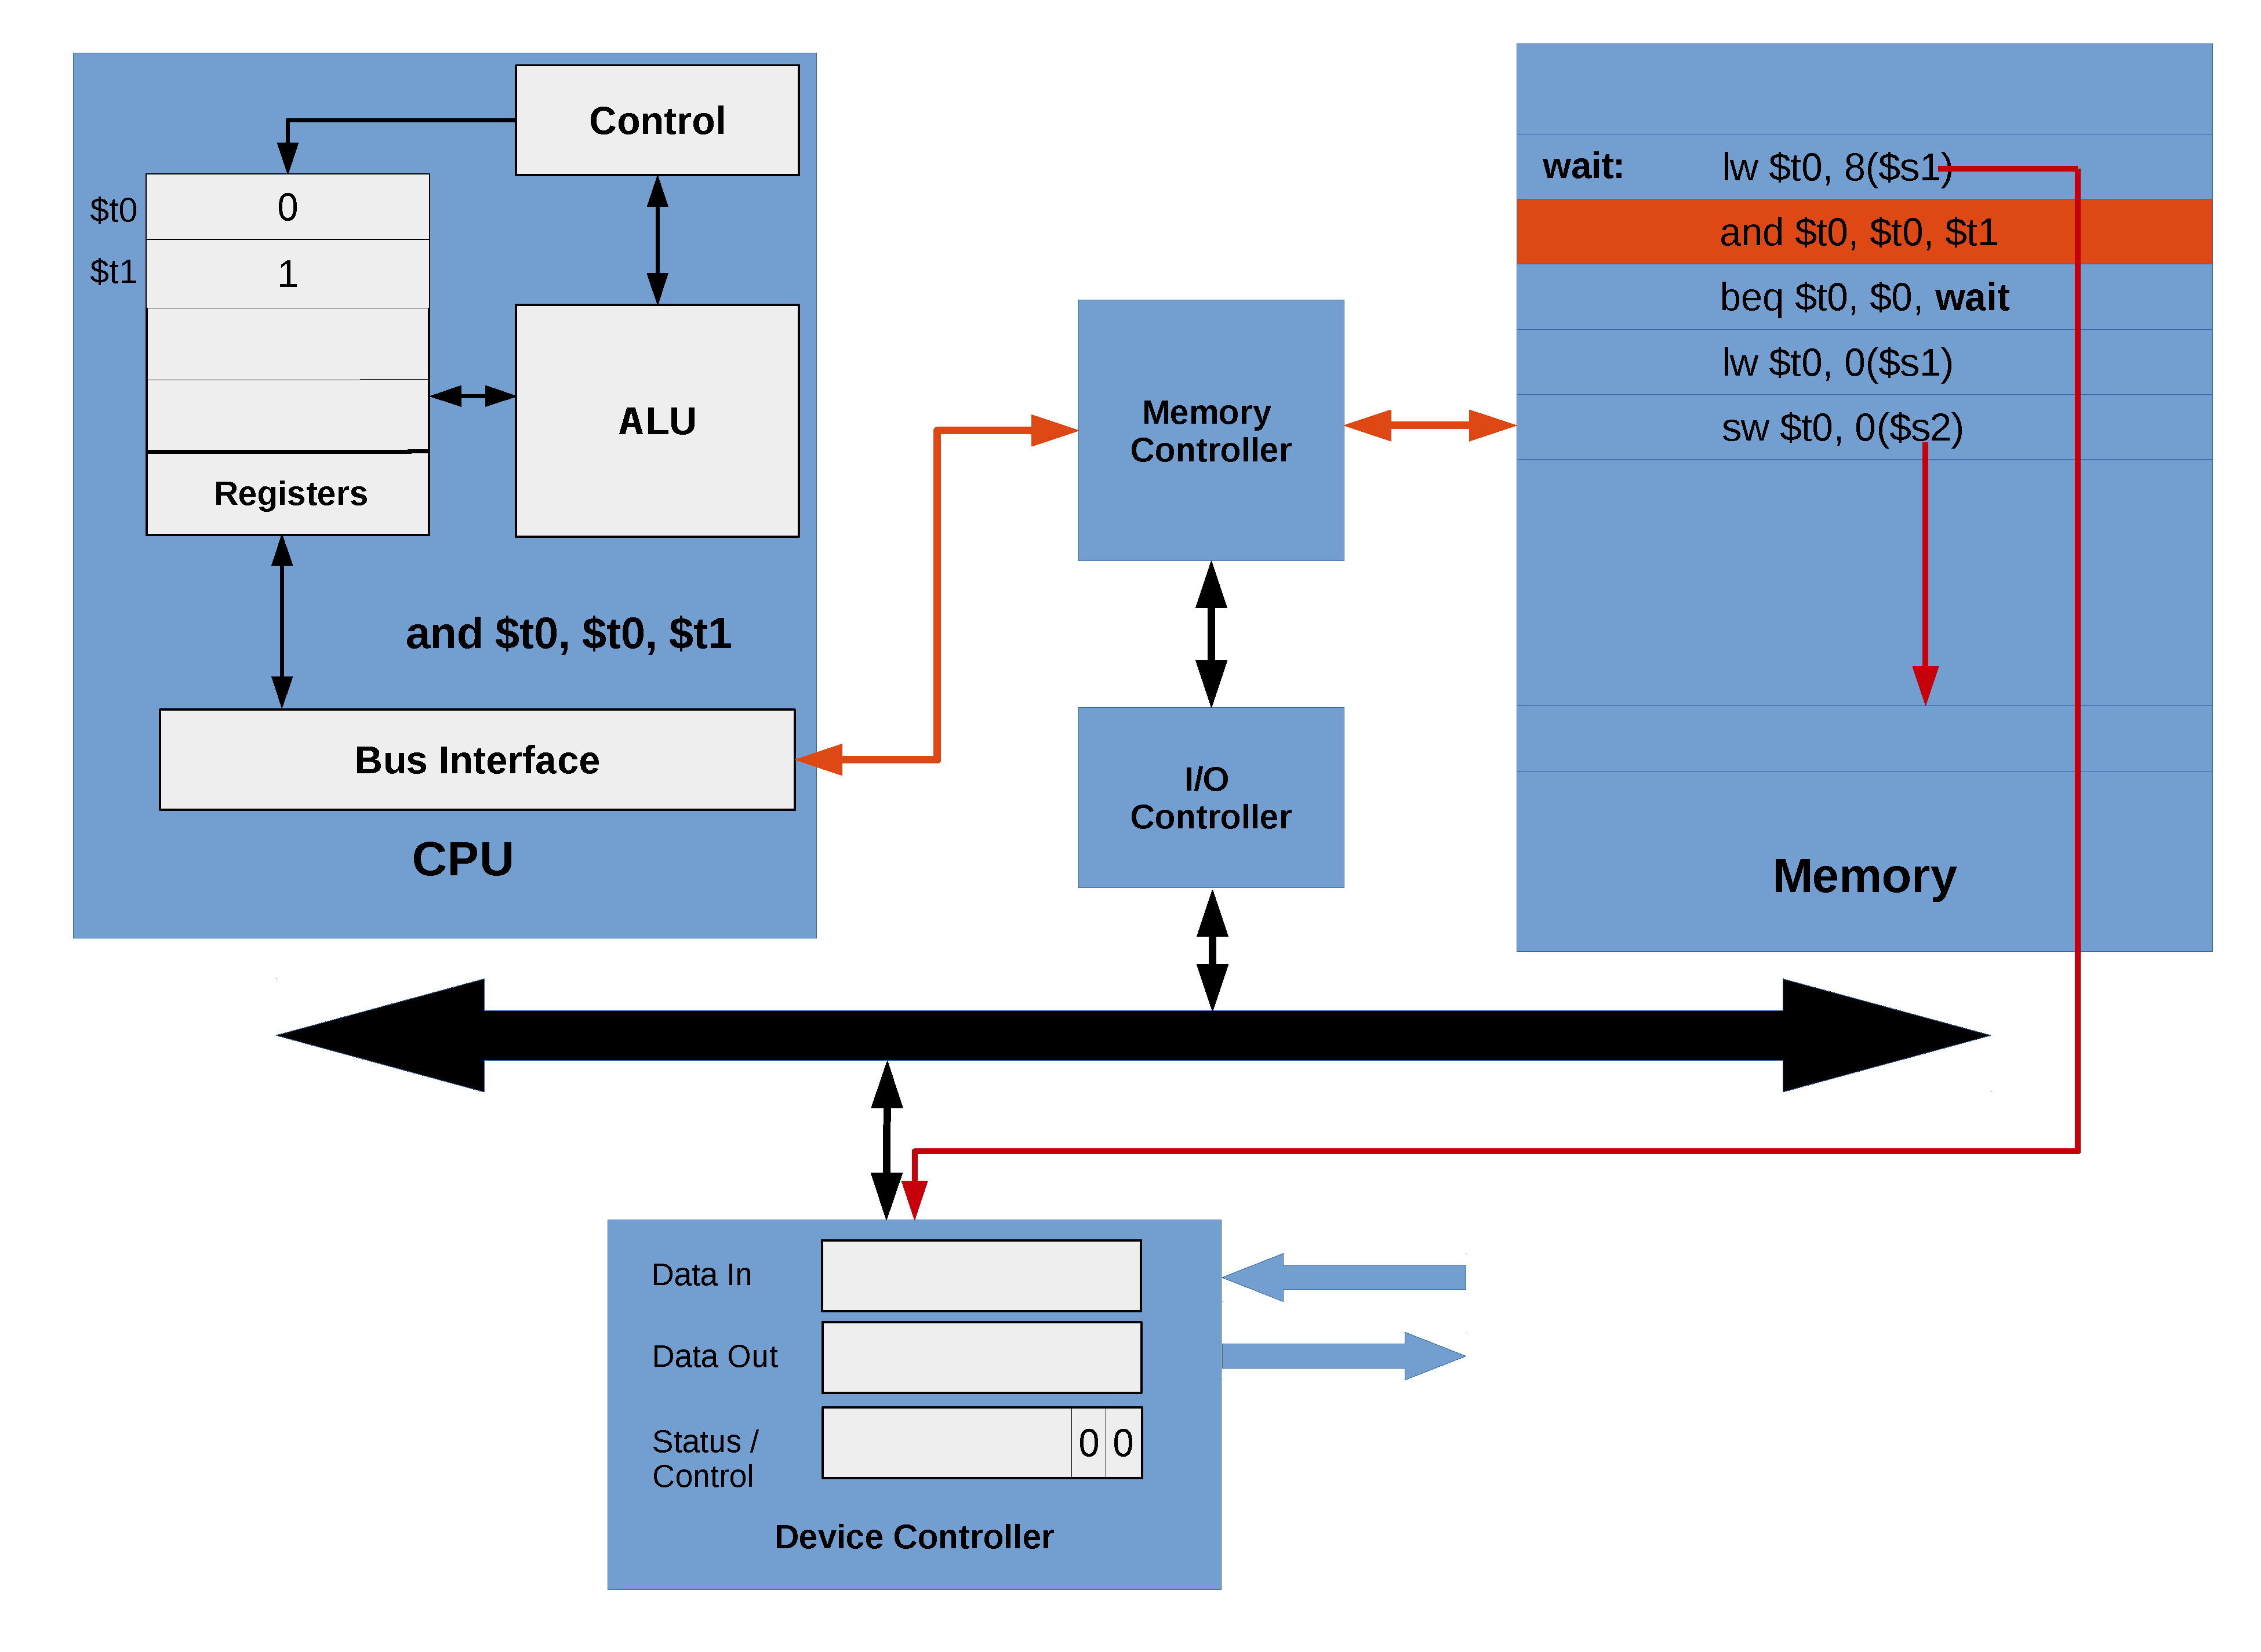
\includegraphics[width=10cm]{busy_waiting5.pdf}
\end{center}

\end{frame}

\begin{frame}%[fragile]
\frametitle{Busy Waiting}

\vspace*{-0.2cm}
\begin{center}
\hspace*{-1cm}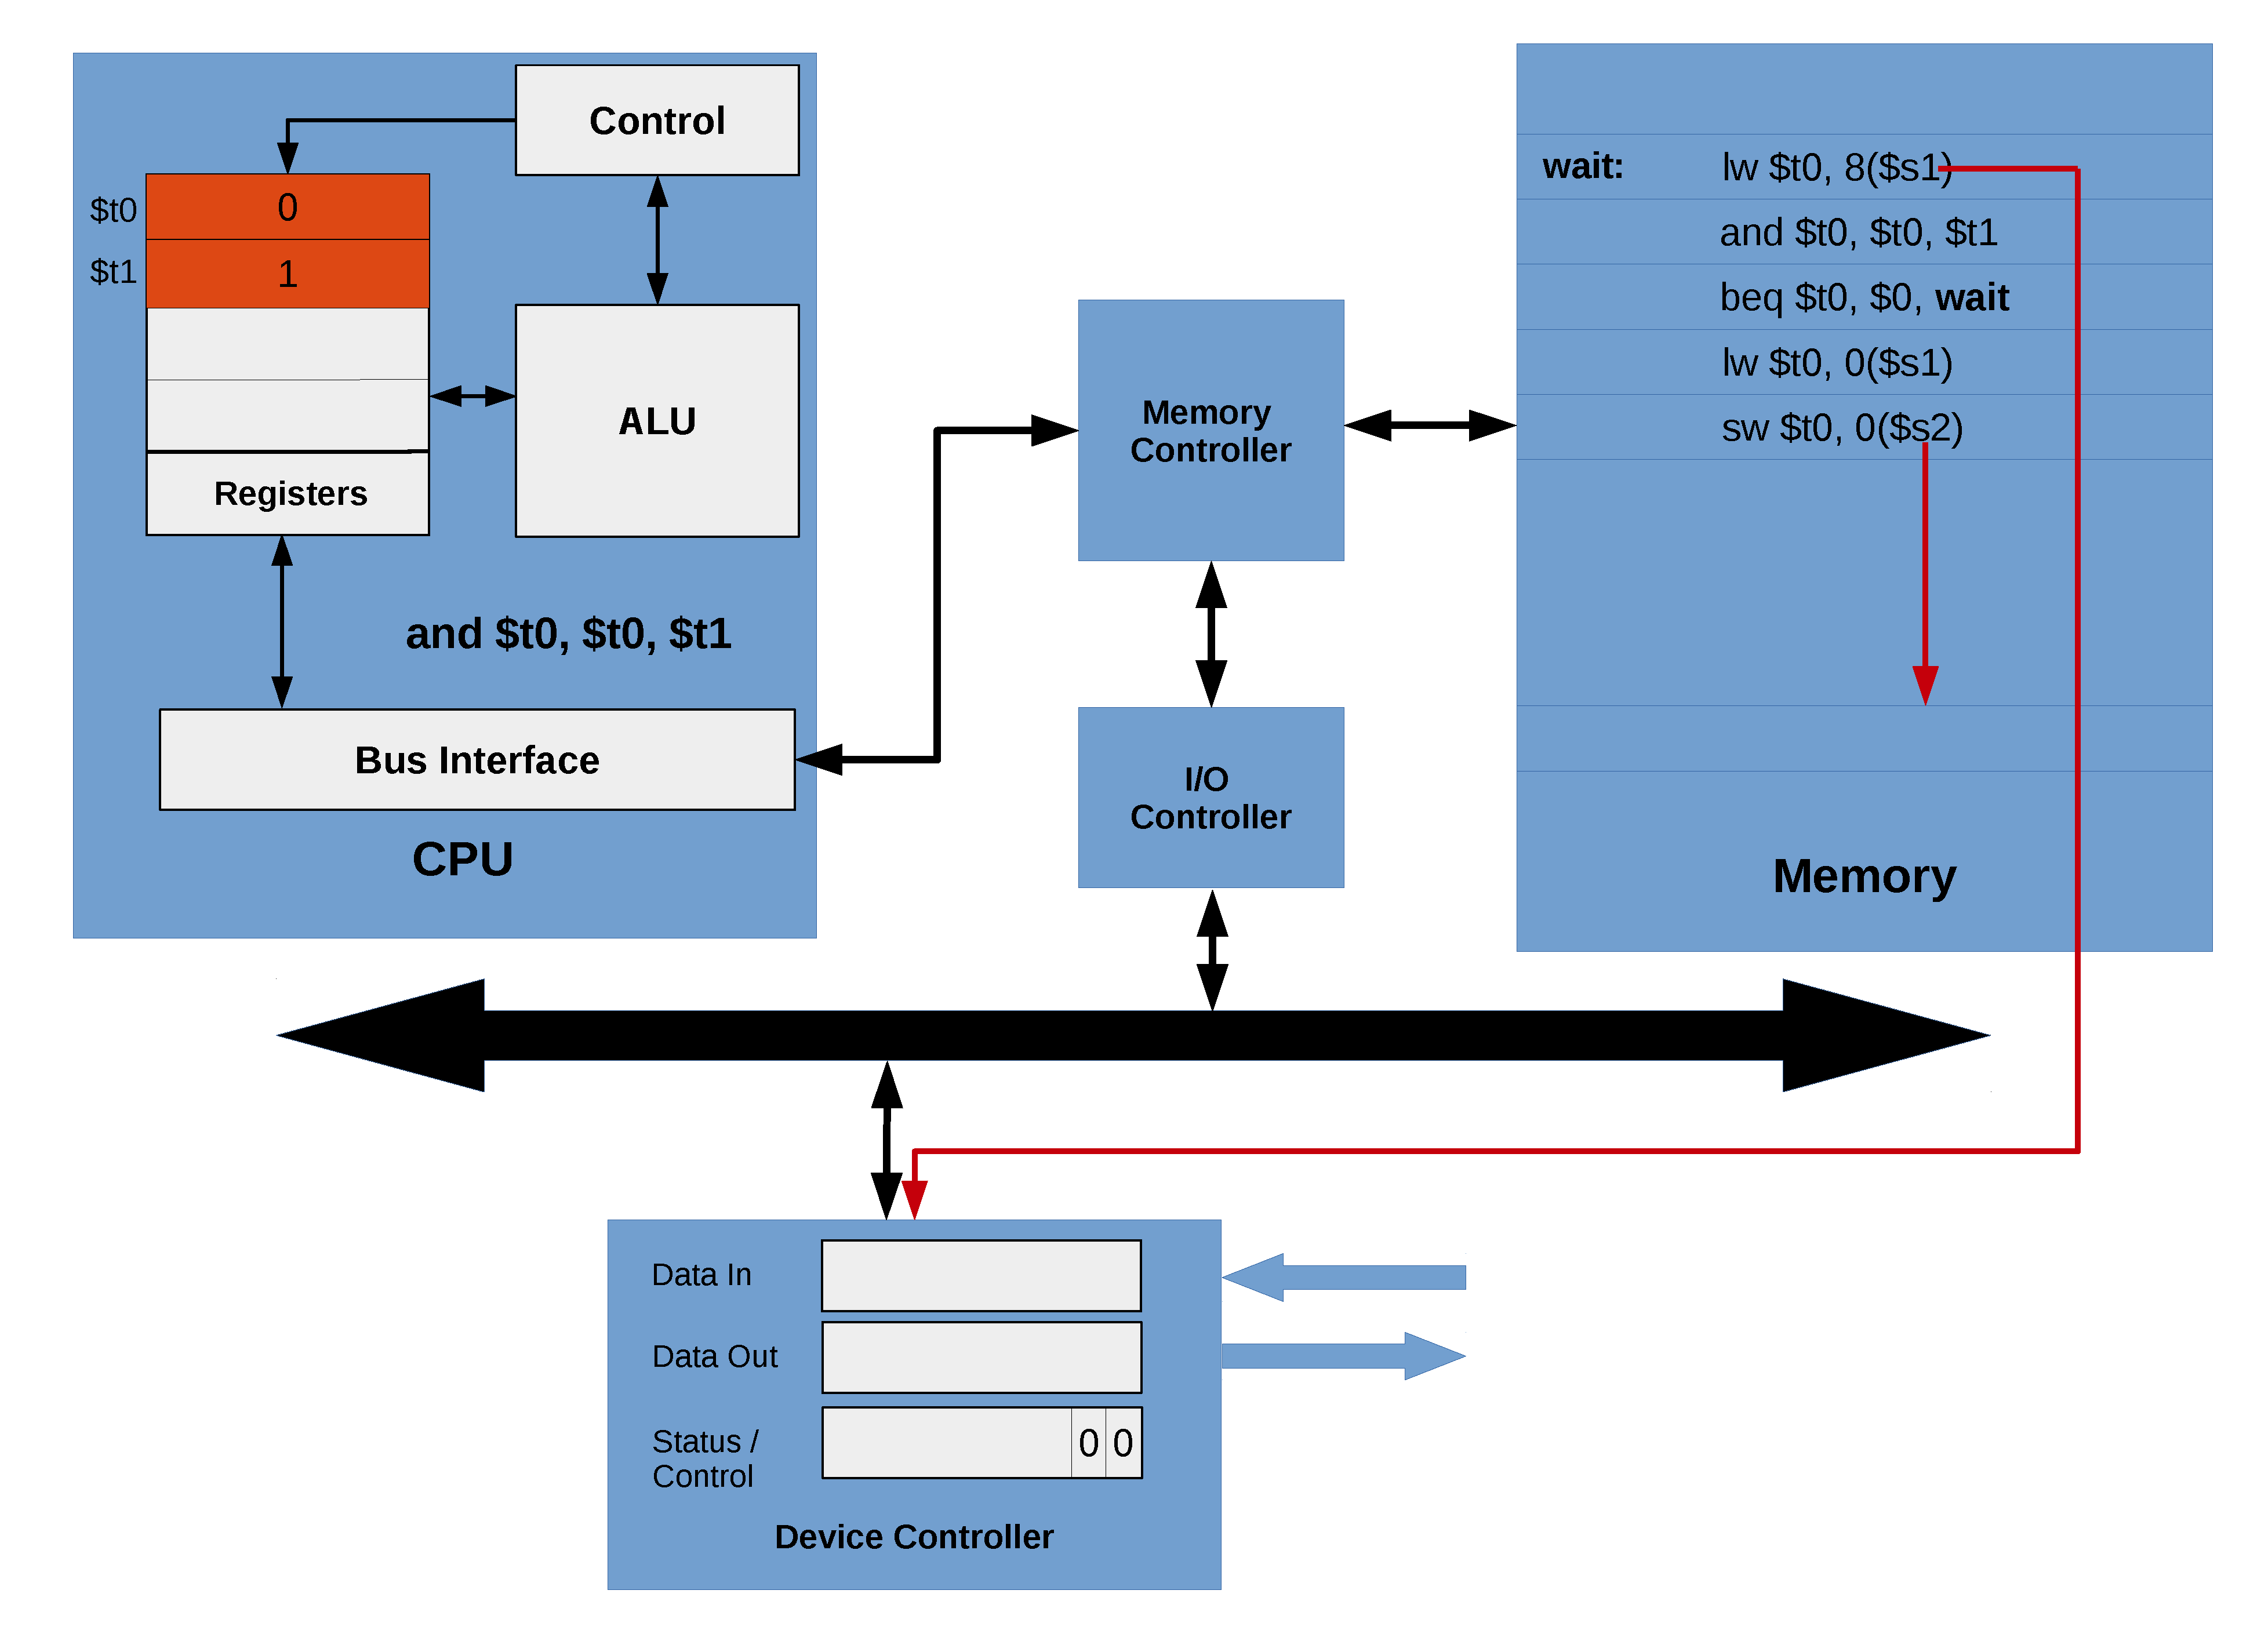
\includegraphics[width=10cm]{busy_waiting6.pdf}
\end{center}

\end{frame}

\begin{frame}%[fragile]
\frametitle{Busy Waiting}

\vspace*{-0.2cm}
\begin{center}
\hspace*{-1cm}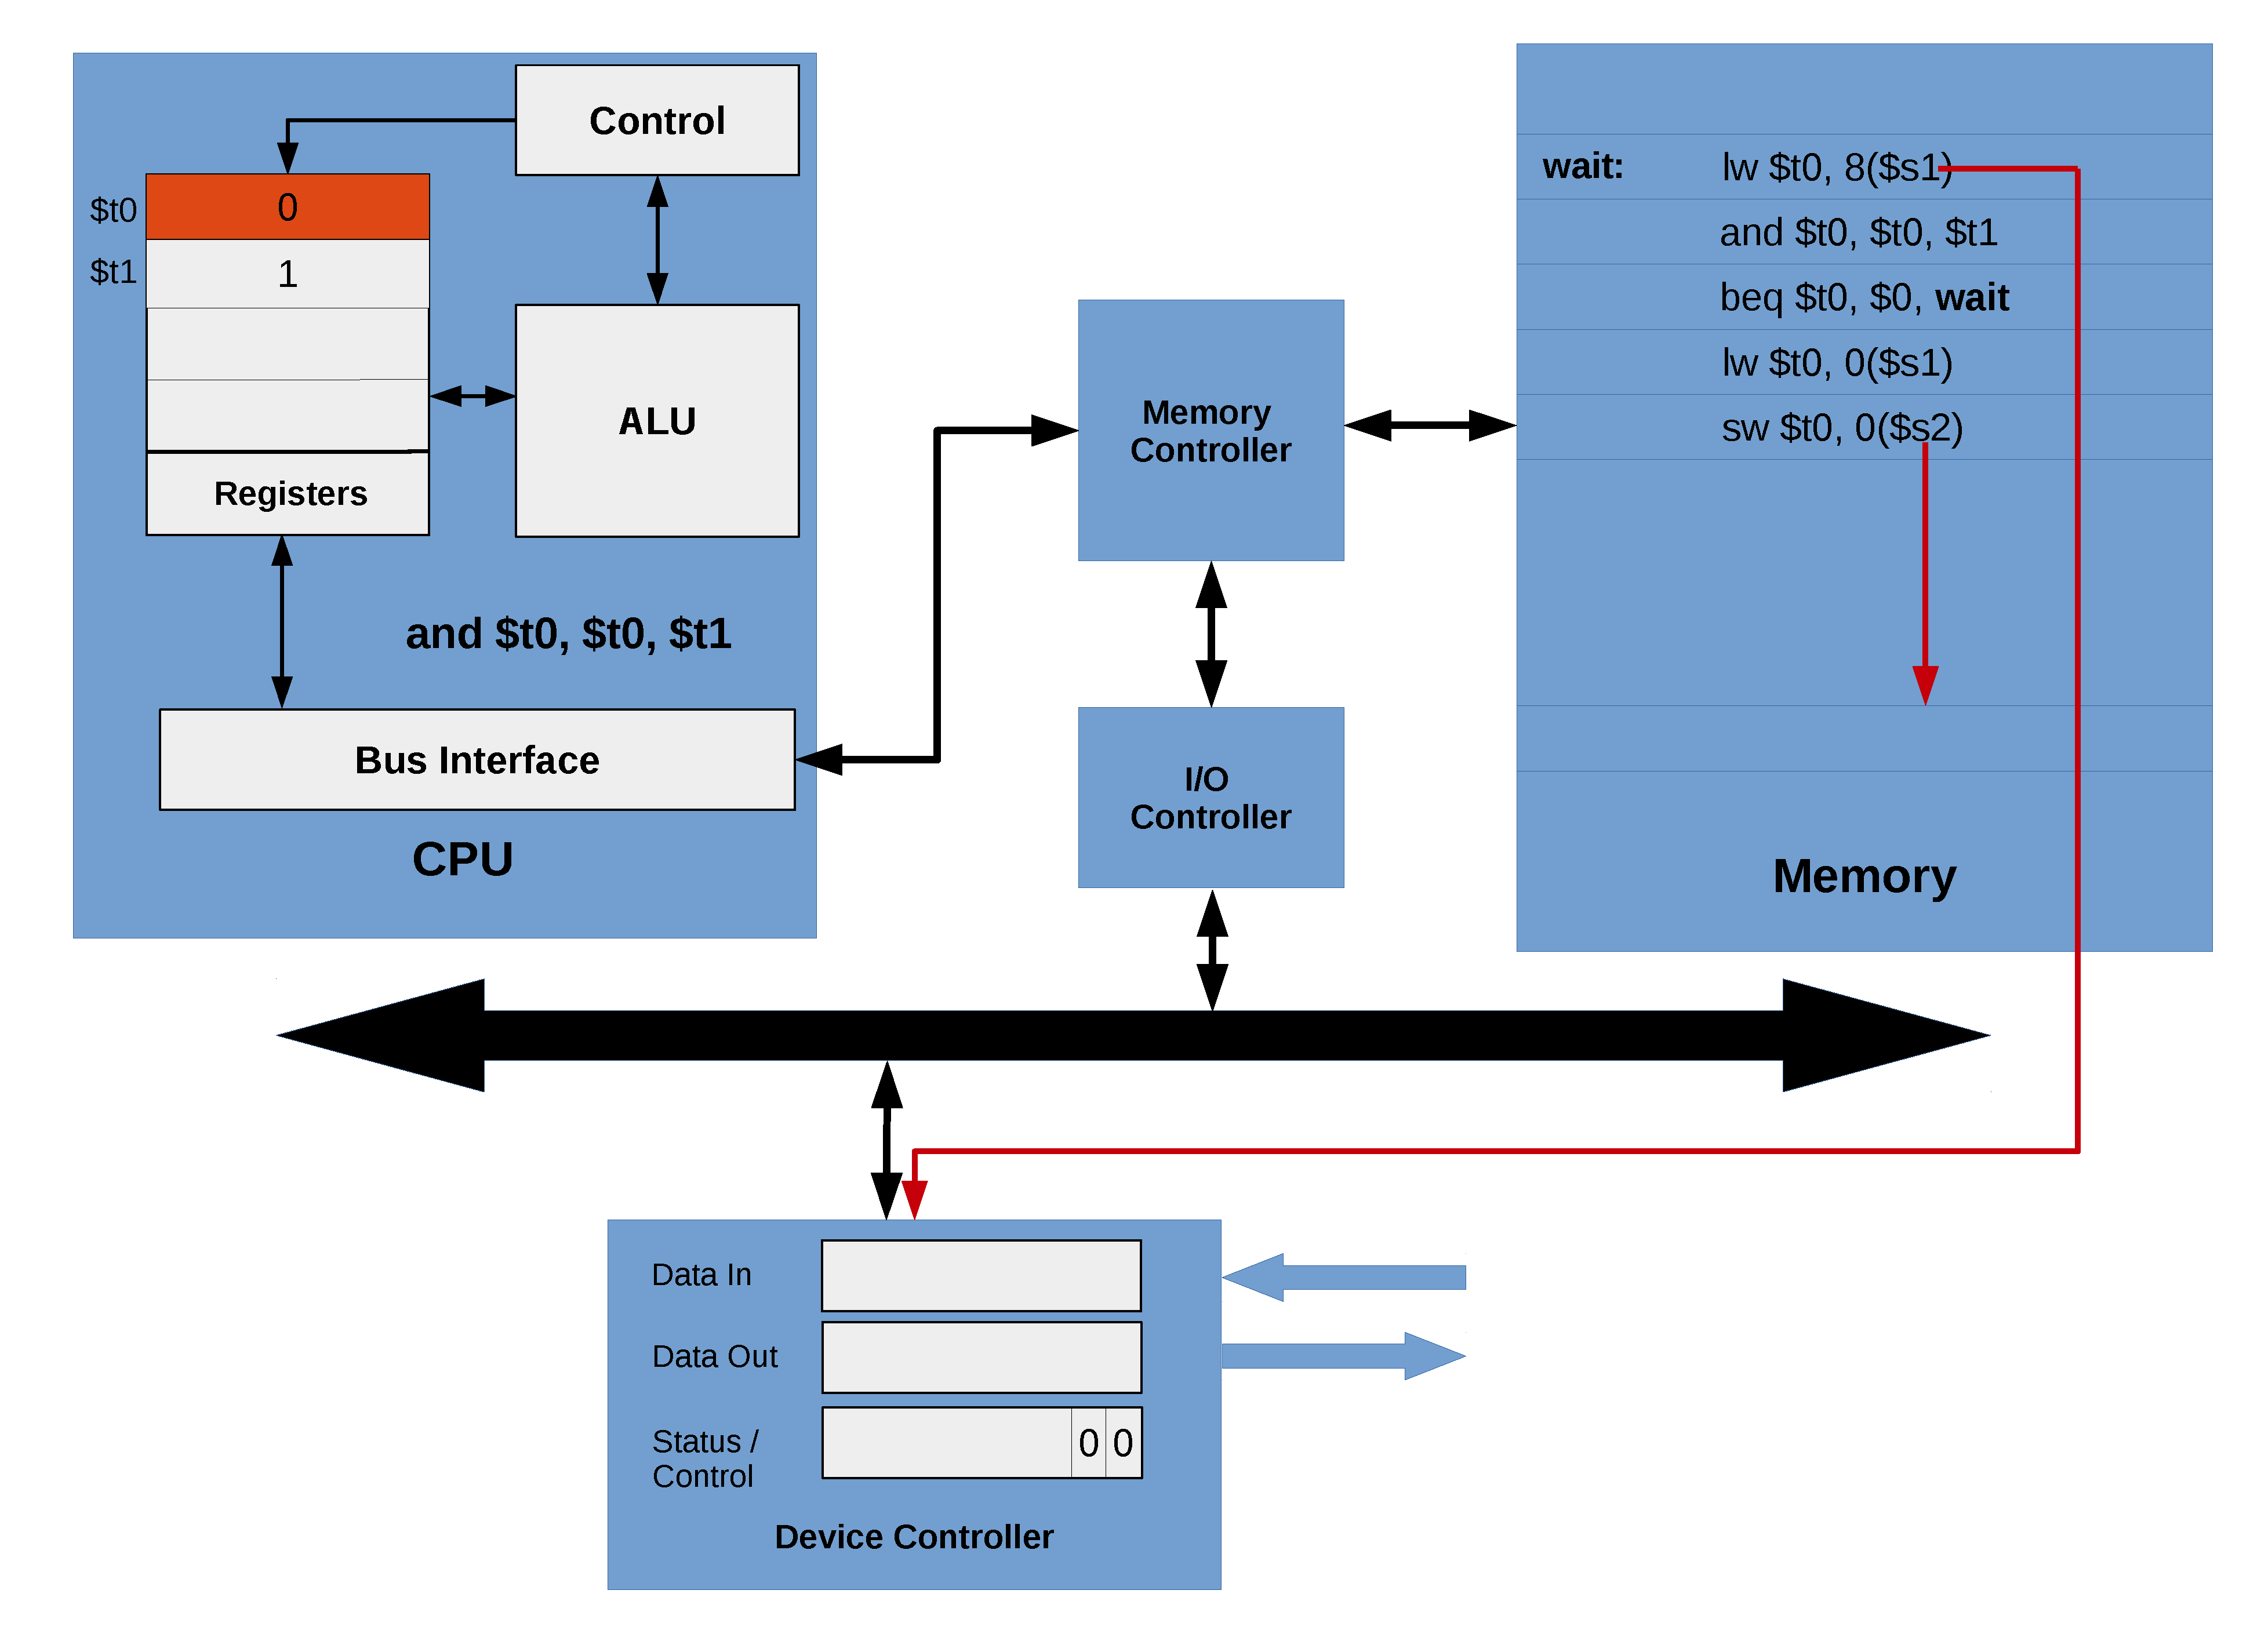
\includegraphics[width=10cm]{busy_waiting7.pdf}
\end{center}

\end{frame}

\begin{frame}%[fragile]
\frametitle{Busy Waiting}

\vspace*{-0.2cm}
\begin{center}
\hspace*{-1cm}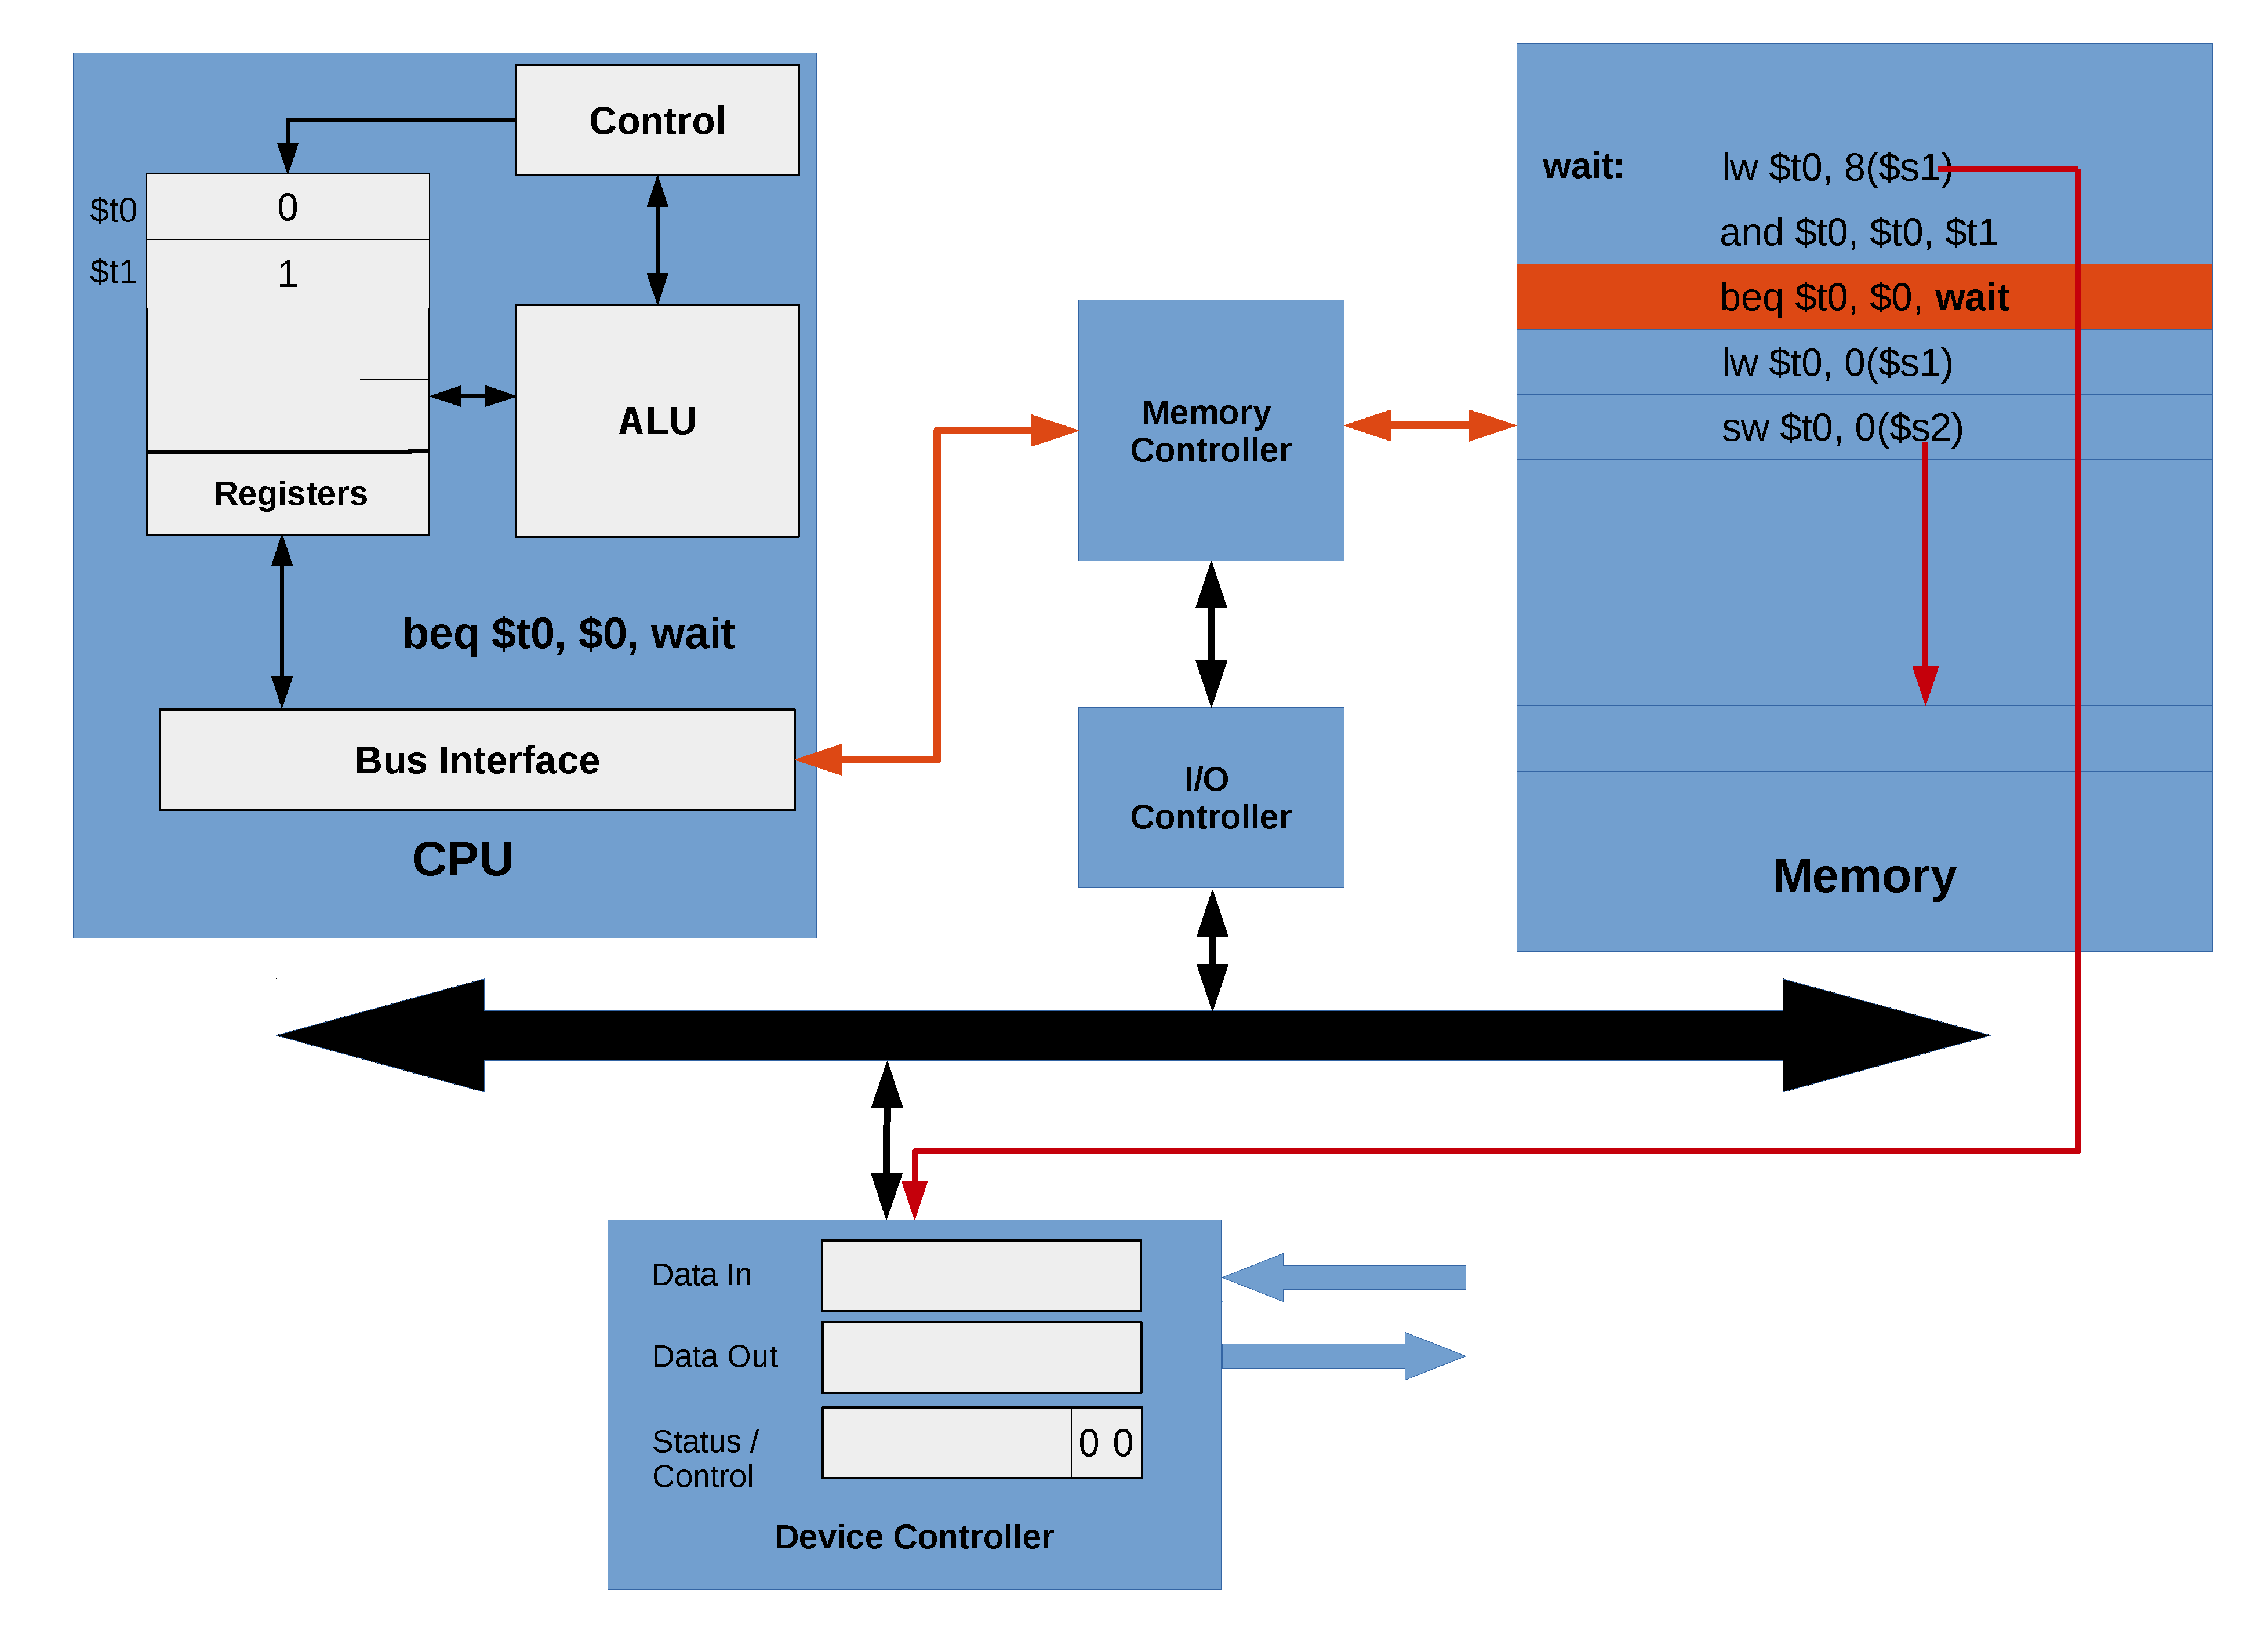
\includegraphics[width=10cm]{busy_waiting8.pdf}
\end{center}

\end{frame}

\begin{frame}%[fragile]
\frametitle{Busy Waiting}

\vspace*{-0.2cm}
\begin{center}
\hspace*{-1cm}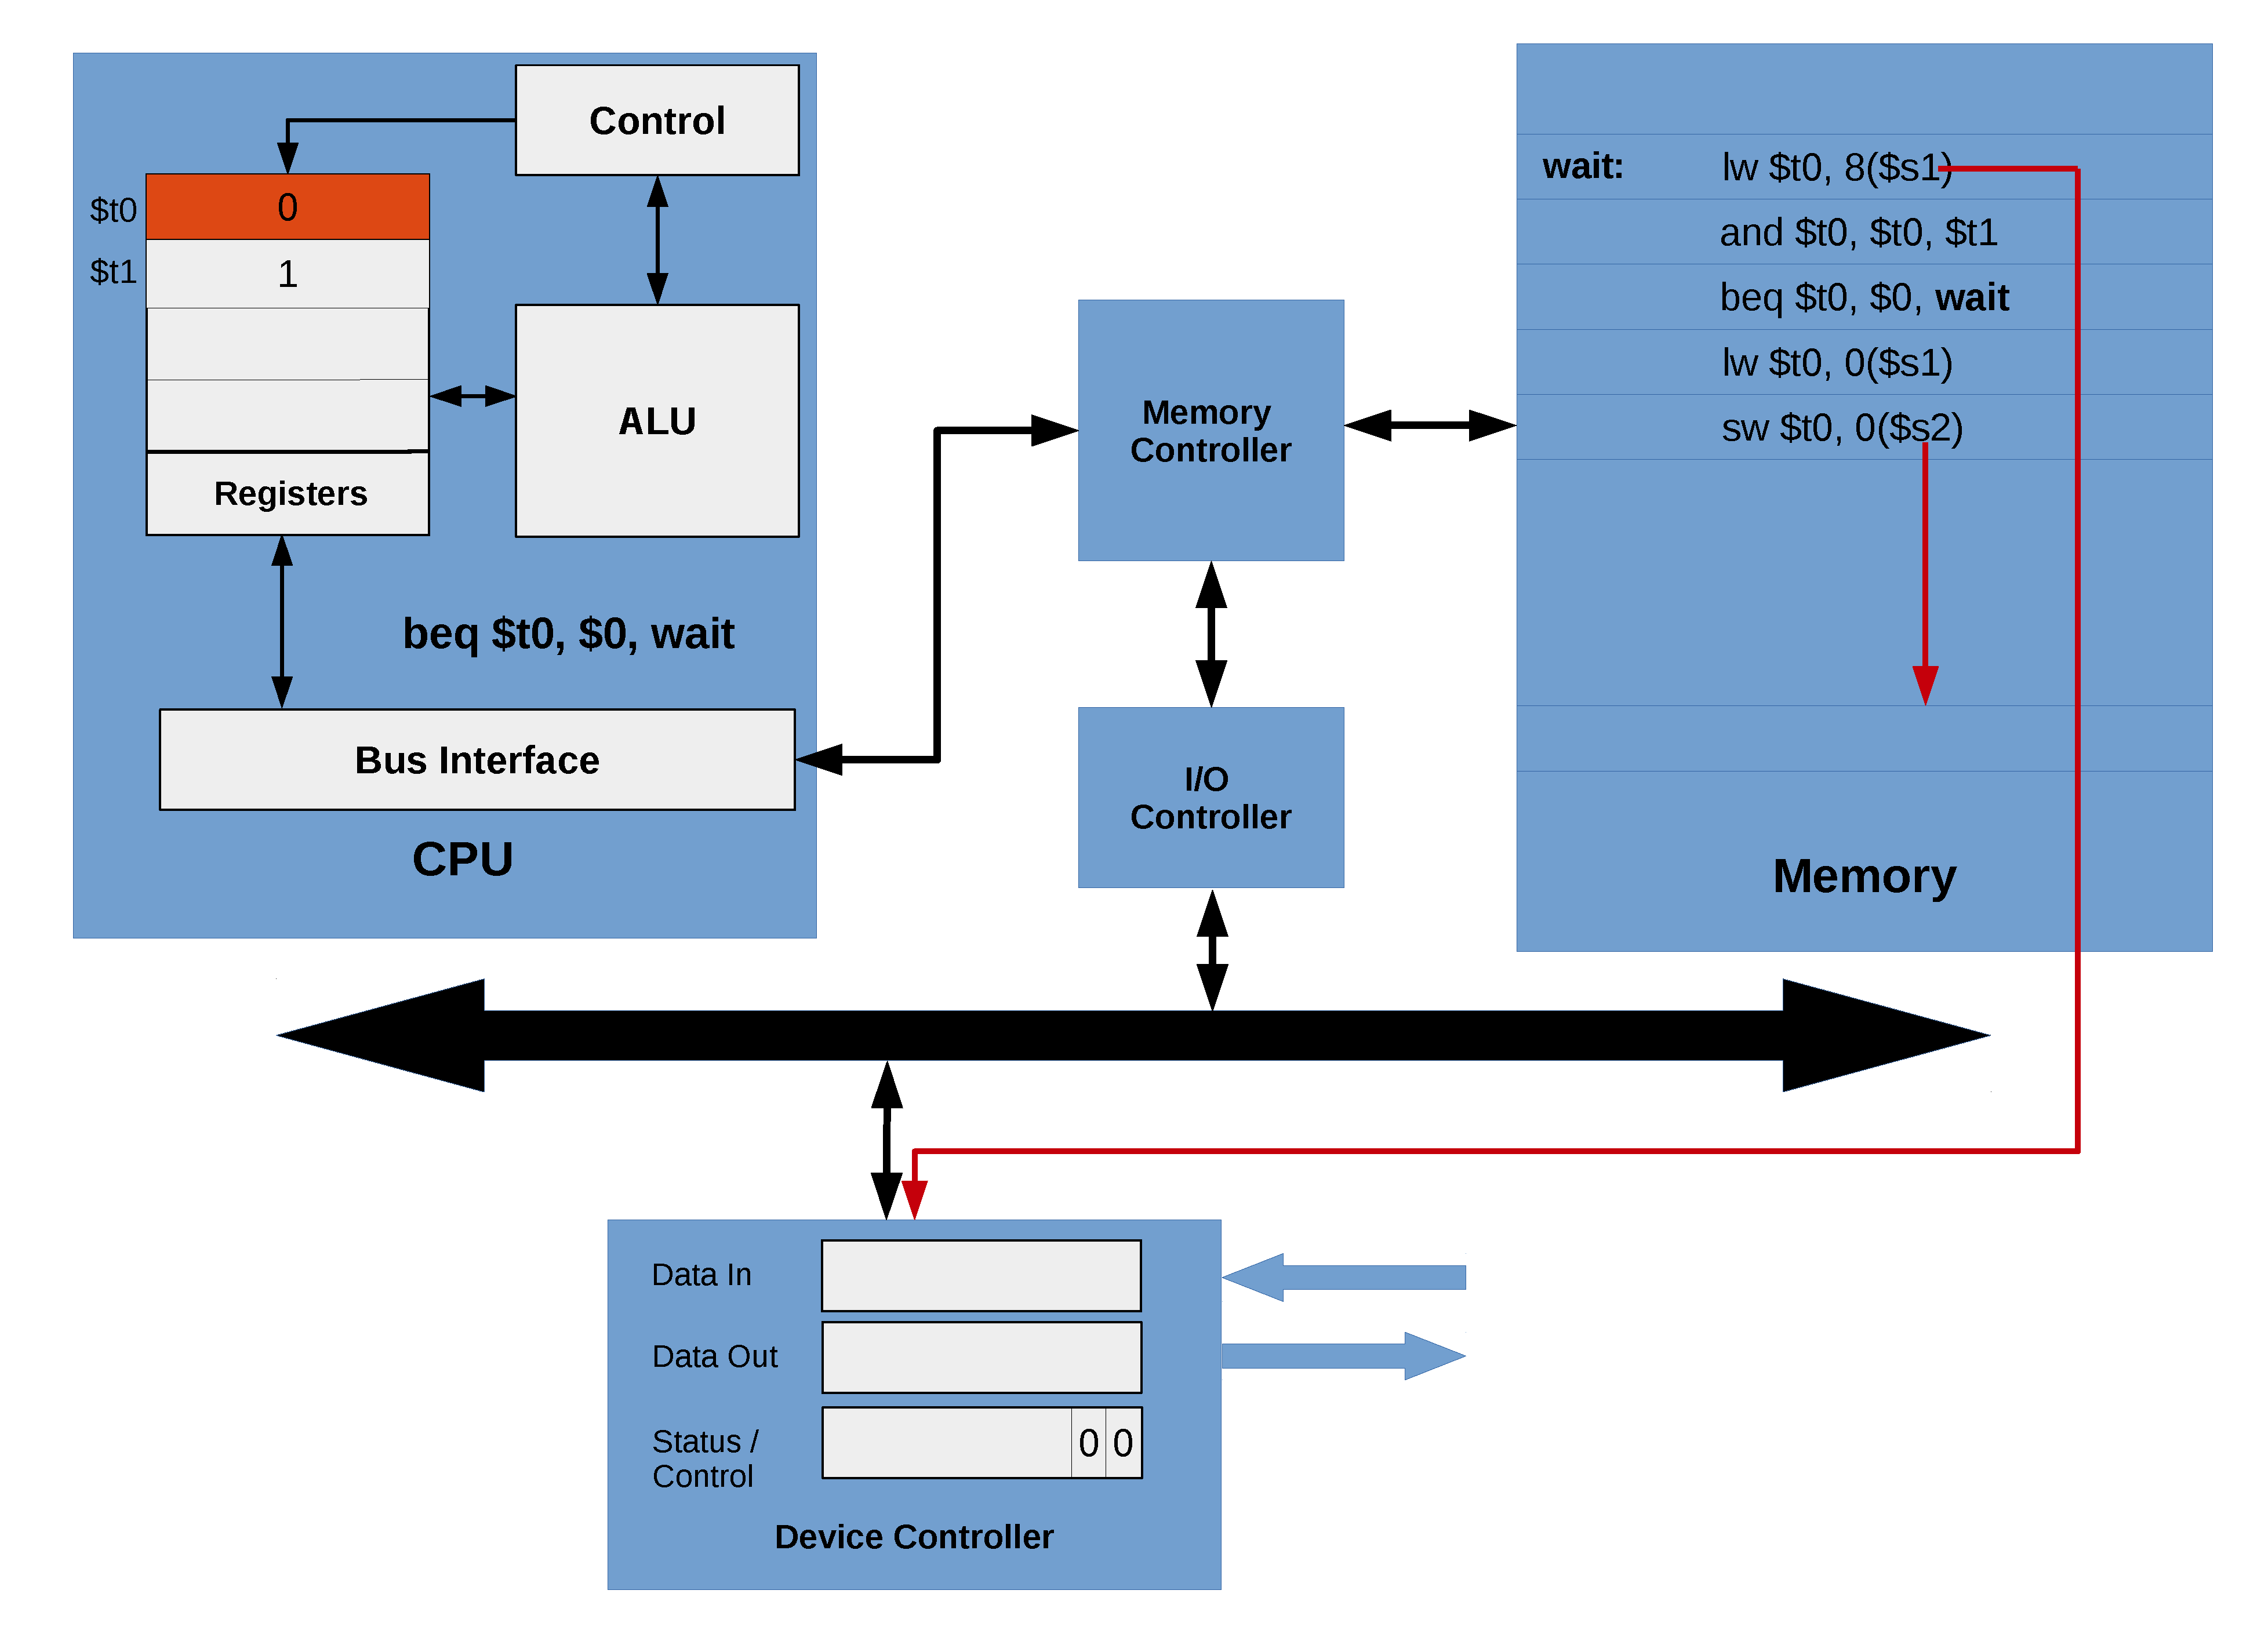
\includegraphics[width=10cm]{busy_waiting8bis.pdf}
\end{center}

\end{frame}

\begin{frame}%[fragile]
\frametitle{Busy Waiting}

\vspace*{-0.2cm}
\begin{center}
\hspace*{-1cm}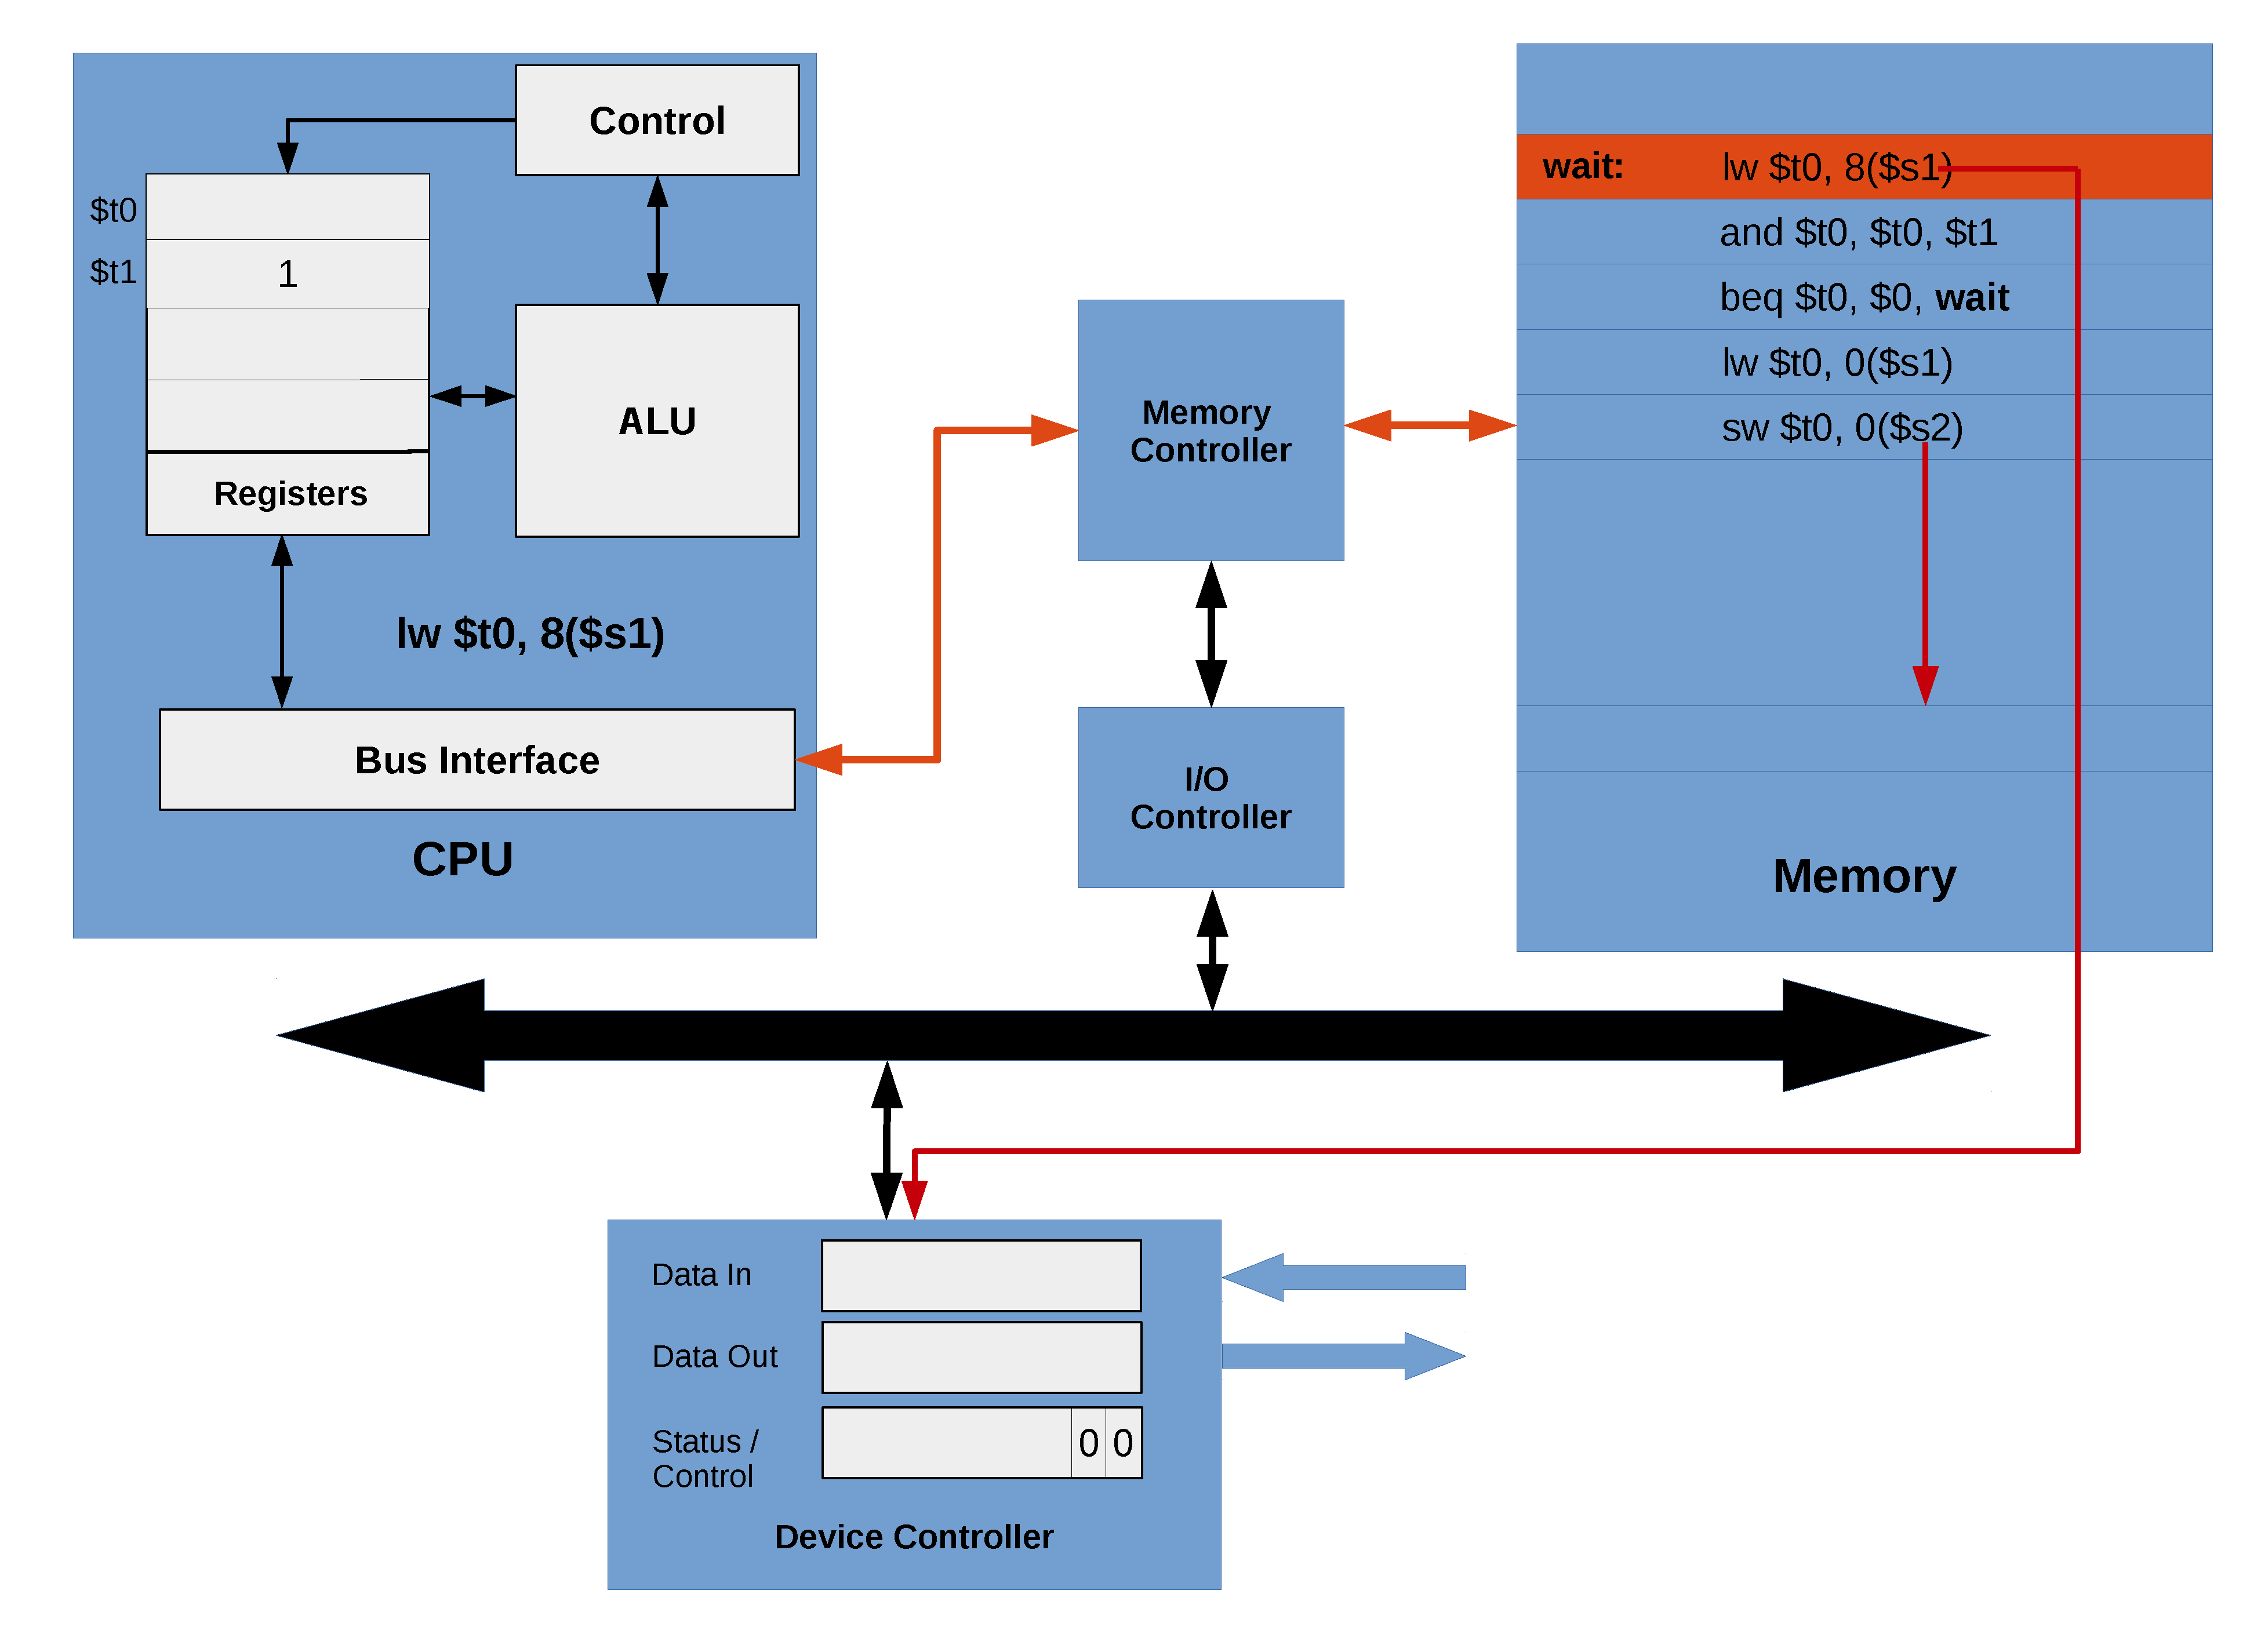
\includegraphics[width=10cm]{busy_waiting3.pdf}
\end{center}

\end{frame}

\begin{frame}%[fragile]
\frametitle{Busy Waiting}

\vspace*{-0.2cm}
\begin{center}
\hspace*{-1cm}\includegraphics[width=10cm]{busy_waiting4.pdf}
\end{center}

\end{frame}

\begin{frame}%[fragile]
\frametitle{Busy Waiting}

\vspace*{-0.2cm}
\begin{center}
\hspace*{-1cm}\includegraphics[width=10cm]{busy_waiting5.pdf}
\end{center}

\end{frame}

\begin{frame}%[fragile]
\frametitle{Busy Waiting}

\vspace*{-0.2cm}
\begin{center}
\hspace*{-1cm}\includegraphics[width=10cm]{busy_waiting6.pdf}
\end{center}

\end{frame}

\begin{frame}%[fragile]
\frametitle{Busy Waiting}

\vspace*{-0.2cm}
\begin{center}
\hspace*{-1cm}\includegraphics[width=10cm]{busy_waiting7.pdf}
\end{center}

\end{frame}

\begin{frame}%[fragile]
\frametitle{Busy Waiting}

\vspace*{-0.2cm}
\begin{center}
\hspace*{-1cm}\includegraphics[width=10cm]{busy_waiting9.pdf}
\end{center}

\end{frame}

\begin{frame}%[fragile]
\frametitle{Busy Waiting}

\vspace*{-0.2cm}
\begin{center}
\hspace*{-1cm}\includegraphics[width=10cm]{busy_waiting10.pdf}
\end{center}

\end{frame}

\begin{frame}%[fragile]
\frametitle{Busy Waiting}

\vspace*{-0.2cm}
\begin{center}
\hspace*{-1cm}\includegraphics[width=10cm]{busy_waiting11.pdf}
\end{center}

\end{frame}

\begin{frame}%[fragile]
\frametitle{Busy Waiting}

\vspace*{-0.2cm}
\begin{center}
\hspace*{-1cm}\includegraphics[width=10cm]{busy_waiting12.pdf}
\end{center}

\end{frame}

\begin{frame}%[fragile]
\frametitle{Busy Waiting}

\vspace*{-0.2cm}
\begin{center}
\hspace*{-1cm}\includegraphics[width=10cm]{busy_waiting13.pdf}
\end{center}

\end{frame}

\begin{frame}%[fragile]
\frametitle{Busy Waiting}

\vspace*{-0.2cm}
\begin{center}
\hspace*{-1cm}\includegraphics[width=10cm]{busy_waiting14.pdf}
\end{center}

\end{frame}

\begin{frame}%[fragile]
\frametitle{Busy Waiting}

\vspace*{-0.2cm}
\begin{center}
\hspace*{-1cm}\includegraphics[width=10cm]{busy_waiting15.pdf}
\end{center}

\end{frame}

\begin{frame}%[fragile]
\frametitle{Busy Waiting}

\vspace*{-0.2cm}
\begin{center}
\hspace*{-1cm}\includegraphics[width=10cm]{busy_waiting16.pdf}
\end{center}

\end{frame}

\begin{frame}%[fragile]
\frametitle{Busy Waiting}

\vspace*{-0.2cm}
\begin{center}
\hspace*{-1cm}\includegraphics[width=10cm]{busy_waiting17.pdf}
\end{center}

\end{frame}

\begin{frame}%[fragile]
\frametitle{Busy Waiting}

\vspace*{-0.2cm}
\begin{center}
\hspace*{-1cm}\includegraphics[width=10cm]{busy_waiting18.pdf}
\end{center}

\end{frame}

\begin{frame}%[fragile]
\frametitle{Busy Waiting}

\vspace*{-0.2cm}
\begin{center}
\hspace*{-1cm}\includegraphics[width=10cm]{busy_waiting19.pdf}
\end{center}

\end{frame}

\begin{frame}%[fragile]
\frametitle{Busy Waiting}

\vspace*{-0.2cm}
\begin{center}
\hspace*{-1cm}\includegraphics[width=10cm]{busy_waiting20.pdf}
\end{center}

\end{frame}

\begin{frame}%[fragile]
\frametitle{Busy Waiting}

\vspace*{-0.2cm}
\begin{center}
\hspace*{-1cm}\includegraphics[width=10cm]{busy_waiting21.pdf}
\end{center}

\end{frame}


\begin{frame}[fragile]
\frametitle{Busy Waiting Problems}

  \scriptsize

\begin{itemize}

\item We waste CPU time to continually check the status register of the device controller.

\vspace{0.2cm}

\item We can miss some data if we apply a long computation to the retrieved data.

  \vspace{0.2cm}

\begin{lstlisting}
# ...
# $t1 = 1
# $t2 = 0xfffffffe
# $s1 = address of device controller
wait:
      lw  $t0, 8($s1)   # get status register
      and $t3, $t0, $t1 # mask receive flag
      beq $t3, $0, wait
      and $t3, $t0, $t2 # reset receive flag
      lw  $a0, 0($s1)   # get data
      sw  $t3, 8($s1)   # set status register
      jal data_handler  # call handler
      j   wait
\end{lstlisting}

\end{itemize}

\end{frame}

\begin{frame}[fragile]
\frametitle{Busy Waiting Problems}

\begin{center}
\vspace*{-0.2cm}
\hspace*{-1cm}\includegraphics[width=13cm]{busy_waiting_problem1.pdf}
\end{center}

\end{frame}

\begin{frame}[fragile]
\frametitle{Getting Notified by Interrupts}


\end{frame}

\begin{frame}[fragile]
\frametitle{Getting Notified by Interrupts}

\begin{center}
\vspace*{-0.23cm}
\hspace*{-1cm}\includegraphics[width=8.7cm]{interrupt_waiting1.pdf}
\end{center}

\end{frame}

\begin{frame}[fragile]
\frametitle{Getting Notified by Interrupts}

\begin{center}
\vspace*{-0.23cm}
\hspace*{-1cm}\includegraphics[width=8.7cm]{interrupt_waiting2.pdf}
\end{center}

\end{frame}

\begin{frame}[fragile]
\frametitle{Getting Notified by Interrupts}

\begin{center}
\vspace*{-0.23cm}
\hspace*{-1cm}\includegraphics[width=8.7cm]{interrupt_waiting3.pdf}
\end{center}

\end{frame}

\begin{frame}[fragile]
\frametitle{Getting Notified by Interrupts}

\begin{center}
\vspace*{-0.23cm}
\hspace*{-1cm}\includegraphics[width=8.7cm]{interrupt_waiting4.pdf}
\end{center}

\end{frame}

\begin{frame}[fragile]
\frametitle{Getting Notified by Interrupts}

\begin{center}
\vspace*{-0.23cm}
\hspace*{-1cm}\includegraphics[width=8.7cm]{interrupt_waiting5.pdf}
\end{center}

\end{frame}

\begin{frame}[fragile]
\frametitle{Getting Notified by Interrupts}

\begin{center}
\vspace*{-0.23cm}
\hspace*{-1cm}\includegraphics[width=8.7cm]{interrupt_waiting6.pdf}
\end{center}

\end{frame}

\begin{frame}[fragile]
\frametitle{Getting Notified by Interrupts}

\begin{center}
\vspace*{-0.23cm}
\hspace*{-1cm}\includegraphics[width=8.7cm]{interrupt_waiting7.pdf}
\end{center}

\end{frame}

\begin{frame}[fragile]
\frametitle{Getting Notified by Interrupts}

\begin{center}
\vspace*{-0.23cm}
\hspace*{-1cm}\includegraphics[width=8.7cm]{interrupt_waiting8.pdf}
\end{center}

\end{frame}

\begin{frame}[fragile]
\frametitle{Getting Notified by Interrupts}

\begin{center}
\vspace*{-0.23cm}
\hspace*{-1cm}\includegraphics[width=8.7cm]{interrupt_waiting9.pdf}
\end{center}

\end{frame}

\begin{frame}[fragile]
\frametitle{Getting Notified by Interrupts}

\begin{center}
\vspace*{-0.23cm}
\hspace*{-1cm}\includegraphics[width=8.7cm]{interrupt_waiting10.pdf}
\end{center}

\end{frame}

\begin{frame}[fragile]
\frametitle{Getting Notified by Interrupts}

\begin{center}
\vspace*{-0.23cm}
\hspace*{-1cm}\includegraphics[width=8.7cm]{interrupt_waiting11.pdf}
\end{center}

\end{frame}

\begin{frame}[fragile]
\frametitle{Getting Notified by Interrupts}

\begin{center}
\vspace*{-0.23cm}
\hspace*{-1cm}\includegraphics[width=8.7cm]{interrupt_waiting12.pdf}
\end{center}

\end{frame}

\begin{frame}[fragile]
\frametitle{Getting Notified by Interrupts}

\begin{center}
\vspace*{-0.23cm}
\hspace*{-1cm}\includegraphics[width=8.7cm]{interrupt_waiting13.pdf}
\end{center}

\end{frame}

\begin{frame}[fragile]
\frametitle{Getting Notified by Interrupts}

\begin{center}
\vspace*{-0.23cm}
\hspace*{-1cm}\includegraphics[width=8.7cm]{interrupt_waiting14.pdf}
\end{center}

\end{frame}

\begin{frame}[fragile]
\frametitle{Getting Notified by Interrupts}

\begin{center}
\vspace*{-0.23cm}
\hspace*{-1cm}\includegraphics[width=8.7cm]{interrupt_waiting15.pdf}
\end{center}

\end{frame}

\begin{frame}[fragile]
\frametitle{Getting Notified by Interrupts}

\begin{center}
\vspace*{-0.23cm}
\hspace*{-1cm}\includegraphics[width=8.7cm]{interrupt_waiting16.pdf}
\end{center}

\end{frame}

\begin{frame}[fragile]
\frametitle{Getting Notified by Interrupts}

\begin{center}
\vspace*{-0.23cm}
\hspace*{-1cm}\includegraphics[width=8.7cm]{interrupt_waiting17.pdf}
\end{center}

\end{frame}

\begin{frame}[fragile]
\frametitle{Getting Notified by Interrupts}

\begin{center}
\vspace*{-0.23cm}
\hspace*{-1cm}\includegraphics[width=8.7cm]{interrupt_waiting18.pdf}
\end{center}

\end{frame}

\begin{frame}[fragile]
\frametitle{Getting Notified by Interrupts}

\begin{center}
\vspace*{-0.23cm}
\hspace*{-1cm}\includegraphics[width=8.7cm]{interrupt_waiting19.pdf}
\end{center}

\end{frame}

\begin{frame}[fragile]
\frametitle{Getting Notified by Interrupts}

\begin{center}
\vspace*{-0.23cm}
\hspace*{-1cm}\includegraphics[width=8.7cm]{interrupt_waiting20.pdf}
\end{center}

\end{frame}

\begin{frame}[fragile]
\frametitle{Getting Notified by Interrupts}

\begin{center}
\vspace*{-0.23cm}
\hspace*{-1cm}\includegraphics[width=8.7cm]{interrupt_waiting21.pdf}
\end{center}

\end{frame}

\begin{frame}[fragile]
\frametitle{Getting Notified by Interrupts}

\begin{center}
\vspace*{-0.23cm}
\hspace*{-1cm}\includegraphics[width=8.7cm]{interrupt_waiting22.pdf}
\end{center}

\end{frame}

\begin{frame}[fragile]
\frametitle{Getting Notified by Interrupts}

\begin{center}
\vspace*{-0.23cm}
\hspace*{-1cm}\includegraphics[width=8.7cm]{interrupt_waiting23.pdf}
\end{center}

\end{frame}

\begin{frame}[fragile]
\frametitle{Getting Notified by Interrupts}

\begin{center}
\vspace*{-0.23cm}
\hspace*{-1cm}\includegraphics[width=8.7cm]{interrupt_waiting24.pdf}
\end{center}

\end{frame}

\begin{frame}[fragile]
\frametitle{Getting Notified by Interrupts}

\begin{center}
\vspace*{-0.23cm}
\hspace*{-1cm}\includegraphics[width=8.7cm]{interrupt_waiting25.pdf}
\end{center}

\end{frame}

\begin{frame}[fragile]
\frametitle{Getting Notified by Interrupts}

\begin{center}
\vspace*{-0.23cm}
\hspace*{-1cm}\includegraphics[width=8.7cm]{interrupt_waiting26.pdf}
\end{center}

\end{frame}

\subsection{Ints and Exceptions on MIPS}

\begin{frame}%[fragile]
\frametitle{MIPS Interrupts and Exceptions}

\begin{itemize}

\item Integer arithmetic and logical operations are executed directly by the CPU
  \vspace{0.3cm}
\item Floating point operations are executed by Coprocessor 1
  \vspace{0.3cm}
\item Coprocessor 0 is used to manage exceptions and interrupts
  \begin{itemize}
    \scriptsize
\item Normal user level code doesn't have access to Coprocessor 0. This is restricted to privileged level code
\item But interrupt and exception aware code has to use it
\item Coprocessor 0 has several registers which controls exceptions and interrupts
  \begin{itemize}
    \scriptsize
  \item The \textcolor{red}{Status} register (number $12$) which manages the exceptions and interrupts behaviour and user or privileged
    level code
  \item The \textcolor{red}{Cause} register (number $13$) which gives information about the cause of the exception or interrupt
  \item The \textcolor{red}{EPC} register (number $14$) which saves the old value of the PC
  \end{itemize}
\end{itemize}

\end{itemize}

\end{frame}

\begin{frame}%[fragile]
\frametitle{Status Register}

\begin{center}
  \includegraphics[width=11cm]{status_register.pdf}
\end{center}

\end{frame}

\begin{frame}%[fragile]
\frametitle{Status Register}

\scriptsize

\begin{itemize}

\item The \textcolor{red}{interrupt mask} field contains a bit for each
  of the six hardware and two software interrupt levels
  \begin{itemize}
    \scriptsize
  \item A mask bit that is \texttt{1} allows interrupts or exceptions at that level to interrupt the processor
  \item A mask bit that is \texttt{0} disallows interrupts or exceptions at that level
  \item When an interrupt or exception arrive, it sets its interrupt pending bit in the Cause register, even if the mask bit is disabled
  \end{itemize}

\vspace{0.2cm}

\item The \textcolor{red}{user mode} bit is \texttt{0} if the processor is running in kernel mode and \texttt{1} if it is
  running in user mode

  \vspace{0.2cm}

\item The \textcolor{red}{exception level} bit is normally \texttt{0}, but is set to
\texttt{1} after an exception or interrupt occur. When this bit is \texttt{1}, interrupts or exceptions are disabled and the
\texttt{EPC} is not updated if another interrupt or exception occur

\vspace{0.2cm}

\item If the \textcolor{red}{interrupt enable} bit is \texttt{1}, interrupts are
allowed. If it is \texttt{0}, they are disabled

\end{itemize}

\end{frame}

\begin{frame}%[fragile]
\frametitle{Cause Register}

\begin{center}
  \includegraphics[width=11cm]{cause_register.pdf}
\end{center}

\end{frame}

\begin{frame}%[fragile]
\frametitle{Cause Register}

\scriptsize

\begin{itemize}

\item The \textcolor{red}{Pending interrupt} bit is set to \texttt{1} when an exception or interrupt is raised at that
  given hardware or software level

\item The \textcolor{red}{Exception code} register describes the cause of an exception through the following codes:

\scriptsize

\begin{center}
\begin{tabular}{|c|c|p{7cm}|}
\hline
Number & Name & Cause\\
\hline
\hline
$0$ & \texttt{Int} & Interrupt (Hardware)\\
\hline
$4$ & \texttt{AdEL} & Address error exception (load or instruction fetch)\\
\hline
$5$ & \texttt{AdES} & Address error exception (store)\\
\hline
$6$ & \texttt{IBE} & Bus error on instructin fetch\\
\hline
$7$ & \texttt{DBE} & Bus error on data load or store\\
\hline
$8$ & \texttt{Sys} & Syscall exception\\
\hline
$9$ & \texttt{Bp} & Breakpoint exception\\
\hline
$10$ & \texttt{RI} & Reserved instruction exception\\
\hline
$11$ & \texttt{CpU} & Coprocessor unimplemented\\
\hline
$12$ & \texttt{Ov} & Arithmetic overflow exception\\
\hline
$13$ & \texttt{Tr} & Trap\\
\hline
$15$ & \texttt{FPE} & Floating point\\
\hline
\end{tabular}
\end{center}

\end{itemize}

\end{frame}

\begin{frame}%[fragile]
\frametitle{Instructions Related to Interrupts and Exceptions}

\begin{itemize}
\item \lstinline{mtc0 reg, dst}: Move the register \lstinline+reg+ to coprocessor 0 register \lstinline+dst+. This instruction can only be used in privileged
  level mode
 \vspace{0.2cm}

\item \lstinline{mfc0 dst, reg}: Move the register \lstinline+reg+ of coprocessor 0 to register \lstinline+dst+. This instruction can only be used in privileged
  level mode
  \vspace{0.2cm}

\item \lstinline{syscall}: Launch the \texttt{Sys} exception. This instruction allows the user to ask service to the operating system
  \vspace{0.2cm}

\item \lstinline{eret}: Set the \texttt{EXL} bit in coprocessor 0's \texttt{Status} register to $0$ and return to the instruction pointed to by
  coprocessor 0's \texttt{EPC} register
\end{itemize}


\end{frame}

\begin{frame}%[fragile]
\frametitle{Interrupt and Exception Sequence}

\begin{itemize}

\item An interrupt is not ignored if the \textcolor{red}{IE} bit is set, the corresponding
  bit in the \textcolor{red}{Interrupt mask} is set and the \textcolor{red}{EXL} bit is unset

\item An exception is not ignored if the corresponding
  bit in the \textcolor{red}{Interrupt mask} is set and the \textcolor{red}{EXL} bit is unset

\item If an interrupt or exception has to be processed, the \texttt{CPU} does the following:
  \begin{itemize}
    \scriptsize

  \item It sets up \textcolor{red}{EPC} to point to the restart location
    \begin{itemize}
      \scriptsize
    \item The current instruction for an exception
    \item The next instruction for an interrupt
  \end{itemize}

\item It sets \textcolor{red}{EXL}, which forces the CPU into kernel (privileged) mode
and disables interrupts and exceptions

\item \textcolor{red}{Cause} is set up so that software can see the reason for the interrupt or exception

\item The CPU then starts fetching instructions from the exception entry point at \texttt{0x80000180}
and everything else is up to software
\end{itemize}

\end{itemize}

\end{frame}


\begin{frame}%[fragile]
\frametitle{Memory Layout of a Program}
\tiny
(From Uppsala university)

\begin{center}
  \includegraphics[width=7cm]{mips_memory_layout.png}
\end{center}

\end{frame}


\begin{frame}%[fragile]
\frametitle{Memory Mapped Console}

\begin{itemize}
\item We will describe one I/O device: A memory-mapped console
  on which a program can read and write characters

\vspace{0.3cm}

\item The terminal device consists of two independent units: A receiver and a transmitter
  \begin{itemize}
  \item The receiver reads characters typed on the keyboard
  \item The transmitter display  characters  on  the  console
  \end{itemize}

  \vspace{0.3cm}

\item The receiver and transmitter are independent. For example, the characters typed at the keyboard are not automatically
echoed on the display

\vspace{0.3cm}

\item A program controls the terminal with four memory-mapped device registers
\end{itemize}

\end{frame}


\begin{frame}%[fragile]
\frametitle{Memory Mapped Registers}

\scriptsize

\begin{center}
  \includegraphics[width=10cm]{terminal.pdf}
\end{center}

\end{frame}

\begin{frame}%[fragile]
  \frametitle{Receiver Control and Status}

  \begin{itemize}
  \item \texttt{Bit 0} is the \texttt{ready} bit
    \begin{itemize}
    \item If it is set to 1, it means that a character has arrived from the keyboard but has not yet been read from the \texttt{Receiver Data} register
    \item It changes from 0 to 1 when a character is typed at the keyboard, and it changes from 1 to 0 when the character is read from the \texttt{Receiver Data} register
    \end{itemize}
    \vspace{0.4cm}
  \item \texttt{Bit 1} is the \texttt{interrupt enable} bit
    \begin{itemize}
    \item If it is set to 1 by a program, the terminal requests an interrupt at hardware level 1 whenever a character is typed and the ready bit becomes 1.
    \item Note that for the interrupt to affect the processor, interrupts must also be enabled in the Status register
    \end{itemize}
  \end{itemize}

\end{frame}

\begin{frame}%[fragile]
  \frametitle{Receiver Data}

  \begin{itemize}
  \item The low-order 8 bits of this register contain the last character typed at the keyboard. All other bits contain 0s
    \vspace{0.2cm}
  \item This register is read-only and changes only when a new character is typed at the keyboard
    \vspace{0.2cm}
  \item Reading the \texttt{Receiver Data} register resets the \texttt{ready} bit in the \texttt{Receiver Control} register to 0
    \vspace{0.2cm}
  \item The value in this register is undefined if the \texttt{Receiver Control} register is 0
  \end{itemize}

\end{frame}

\begin{frame}%[fragile]
  \frametitle{Transmitter Control and Status}

  \begin{itemize}
  \item \texttt{Bit 0} is the \texttt{ready} bit
    \begin{itemize}
    \item If this bit is 1, the transmitter is ready to accept a new character for output
    \item If it is 0, the transmitter is still busy writing the previous character
    \end{itemize}
    \vspace{0.4cm}
  \item \texttt{Bit 1} is the \texttt{interrupt enable} bit
    \begin{itemize}
    \item If this bit is set to 1, then the terminal requests an interrupt at hardware level 0 whenever the transmitter
      is ready for a new character and the ready bit becomes 1
    \end{itemize}
  \end{itemize}

\end{frame}

\begin{frame}%[fragile]
  \frametitle{Transmitter Data}

  \begin{itemize}
  \item When a value is written into this location, its low-order 8 bits (i.e., an ASCII character) are sent to the console

  \item When the \texttt{Transmitter Data} register is written, the \texttt{ready} bit in the \texttt{Transmitter Control} register is reset to 0.\\
    This bit stays 0 until enough time has elapsed to transmit the character to the terminal; then the \texttt{ready} bit becomes 1 again

  \item Reading the \texttt{Receiver Data} register resets the \texttt{ready} bit in the \texttt{Receiver Control} register to 0

  \item The \texttt{Transmitter Data} register should only be written when the ready bit of the
    \texttt{Transmitter Control} register is 1. If the transmitter is not ready, writes to the \texttt{Transmitter Data} register are ignored
  \end{itemize}

\end{frame}


\lstset{language=[mips]Assembler}
\begin{frame}[fragile]
\frametitle{Program Echoing Characters}

\scriptsize

The following program echoes characters from keyboard to screen.

\begin{lstlisting}
###############################################################
# User text
# MARS start to execute at label main in the user .text segment
###############################################################
  .globl main
  .text
main:
  # Enable keyboard interrupts
  lw $s0, 0xffff0000
  ori $s1, $s0, 2
  sw $s1, 0xffff0000
loop:
  # This infinite loop simulates the CPU doing something useful such as
  # executing another job while waiting for user keyboard input
  addi $s0, $s0, 1
  j loop
\end{lstlisting}

\end{frame}

\begin{frame}[fragile]
\frametitle{Program Echoing Characters}

\scriptsize

\begin{lstlisting}[firstnumber=17]
###############################################################
# Kernel data and code
###############################################################
  .kdata
__save0: .word 0
__save1: .word 0
  .ktext 0x80000180 # The handler address for MIPS32
__handler:
  sw   $at, __save0
  mfc0 $k0, $13 # Get value in cause register
  andi $k1, $k0, 0x00007c # Mask all but the exception code to zero
  srl  $k1, $k1, 2 # Shift to get the exception code
  # Now $k0 = value of cause register
  #     $k1 = exception code
  # The exception code is zero for an interrupt
  beqz $k1, __interrupt
__unhandled_exception:
  j __resume_exception
\end{lstlisting}

\end{frame}

\begin{frame}[fragile]
\frametitle{Program Echoing Characters}

\scriptsize

\begin{lstlisting}[firstnumber=35]
__interrupt:
  andi $k1, $k0, 0x00000100 # Reset interrupt pending bit
  # Shift the interrupt pending bit as the least significant bit
  srl  $k1, $k1, 8
  beq  $k1, 1, __keyboard_interrupt # Branch on the interrupt pending
  j __resume
__keyboard_interrupt:
  # Get ASCII value of pressed key from the receiver data register
  # Store content of the memory mapped receiver data register in $k1
  lw $k1, 0xffff0004
  sw $k0, __save1
__wait:
  lw $k0, 0xffff0008 # Busy wait for console ready to accept data
  andi $k0, 1
  beqz $k0, __wait
  sw $k1, 0xffff000c
  lw $k0, __save1
  j __resume
\end{lstlisting}

\end{frame}

\begin{frame}[fragile]
\frametitle{Program Echoing Characters}

\scriptsize

\begin{lstlisting}[firstnumber=53]
__resume_exception:
  # When an exception or interrupt occurs, the value of the program
  # counter ($pc) of the user level program is automatically stored
  # in the exception program counter (ECP), the register $14 in
  # Coprocessor 0
  # Get value of EPC (Address of instruction causing the exception)
  mfc0 $k0, $14
  # Skip offending instruction by adding 4 to the value stored in EPC
  # Otherwise the same instruction would be executed again causing the
  # same exception again
  addi $k0, $k0, 4
  mtc0 $k0, $14 # Update EPC in coprocessor 0
  __resume:
  mtc0 $0, $13 # Clear cause register
  lw $at, __save0
  eret
\end{lstlisting}

\end{frame}

\begin{frame}%[fragile]
\frametitle{Simplified MIPS Interrupts and Exceptions}

TO DO

\end{frame}

\subsection{Single-Cycle with Ints and Exs}

\begin{frame}%[fragile]
\frametitle{Single-Cycle Datapath with Interrupts and Exceptions}

\begin{center}
\vspace*{-0.2cm}
\hspace*{-1cm}\includegraphics[width=11.1cm]{complete_single_cycle_int.pdf}
\end{center}

\end{frame}

\subsection{Ints and Exceptions on x86\_64}

\begin{frame}%[fragile]
\frametitle{x86\_64 Interrupts and Exceptions}


\end{frame}


\subsection{Linux Signals}

\begin{frame}%[fragile]
\frametitle{Linux Signals}


\end{frame}

\lstset{language = c++, frameround = fttt, frame=trBL}

\begin{frame}[fragile]
\frametitle{Find the Bug}
\scriptsize

\begin{lstlisting}
#include <stdio.h>
#include <stdlib.h>
#include <signal.h>
#include <sys/time.h>

#define BUFFER_SIZE 1024
int buffer[BUFFER_SIZE];
volatile int head  = 0;
volatile int size  = 0;
volatile int counter = 0;

void producer(int signo)
{
  if (size < BUFFER_SIZE)
    {
      buffer[(head + size) % BUFFER_SIZE] = counter++;
      ++size;
    }
}
\end{lstlisting}

\end{frame}

\begin{frame}[fragile]
\frametitle{Find the Bug}
\scriptsize

\begin{lstlisting}[firstnumber=20]
void consumer()
{
  static int last_data = -1;
  if (size == 0) return;
  int data = buffer[head];
  head = (head + 1) % BUFFER_SIZE;
  --size;
  if (last_data != data)
    {
      printf("%d\n", data);
      last_data = data;
    }
}
\end{lstlisting}

\end{frame}

\begin{frame}[fragile]
\frametitle{Find the Bug}
\scriptsize

\begin{lstlisting}[firstnumber=33]
int check_consistency()
{
  for (int i = head; i < head + size - 1; ++i)
    {
      if (buffer[i % BUFFER_SIZE] + 1 !=
          buffer[(i + 1) % BUFFER_SIZE])
        return 0;
    }
  return 1;
}
\end{lstlisting}

\end{frame}

\begin{frame}[fragile]
\frametitle{Find the Bug}
\scriptsize

\begin{lstlisting}[firstnumber=43]
int main() {
  struct itimerval delay;
  signal(SIGALRM, producer);
  delay.it_value.tv_sec = 0;
  delay.it_value.tv_usec = 10;
  delay.it_interval.tv_sec = 0;
  delay.it_interval.tv_usec = 10;
  if (setitimer(ITIMER_REAL, &delay, NULL))
    {
      perror("setitimer");
      return EXIT_FAILURE;
    }
  while (check_consistency())
    {
      consumer();
    }
  printf("Something has gone wrong\n");
  return EXIT_SUCCESS;
}
\end{lstlisting}

\end{frame}

\begin{frame}[fragile]
\frametitle{Find the Bug}
\scriptsize

\begin{lstlisting}
// gcc -O3 signal.c -o signal && ./signal

// ...
// 58051
// 58052
// 58053
// 58054
// 58055
// 58056
// 58057
// 58058
// 58059
// 58060
// 58061
// 58062
// 58063
// 58064
// 58065
// Something has gone wrong
\end{lstlisting}

\end{frame}

\ifanswers

\begin{frame}[fragile]
\frametitle{Solution}
\scriptsize

\begin{lstlisting}[linebackgroundcolor={\lstcolorlines{6, 9}}]
void consumer()
{
  static int last_data = -1;
  if (size == 0) return;
  int data = buffer[head];
  mask_signal();
  head = (head + 1) % BUFFER_SIZE;
  --size;
  unmask_signal();
  if (last_data != data)
    {
      printf("%d\n", data);
      last_data = data;
    }
}
\end{lstlisting}

\end{frame}

\begin{frame}[fragile]
\frametitle{Solution}
\scriptsize

\begin{lstlisting}
void mask_signal()
{
  sigset_t set;
  sigset_t old;
  sigemptyset(&set);
  sigaddset(&set, SIGALRM);
  sigprocmask(SIG_SETMASK, &set, &old);
}

void unmask_signal()
{
  sigset_t set;
  sigemptyset(&set);
  sigprocmask(SIG_SETMASK, &set, NULL);
}
\end{lstlisting}

\end{frame}

\fi

\section{Out of Order}

\begin{frame}%[fragile]
\frametitle{Out of Order}

\end{frame}

\section{Memory Hierarchy}

\subsection{Overview}

\begin{frame}%[fragile]
\frametitle{Memory Hierarchy}

\scriptsize

\begin{itemize}

\item Problem: Large memory access time is way bigger than the clock cycle time of the processor

%\vspace{0.5cm}

\item Problem: Fast memory technology is more expensive per bit than slower memory

 % \vspace{0.5cm}

\item What we want: A big fast and cheap memory!

%\vspace{0.5cm}

\item Because of locality of memory references, we can build a memory hierarchy to obtain the illusion
  of a fast, big and cheap memory

  \vspace{0.25cm}

\begin{center}
\includegraphics[width=6cm]{memhier.pdf}
\end{center}


\end{itemize}

\end{frame}

\begin{frame}%[fragile]
\frametitle{Memory Latency}
\tiny
(From \emph{Computer Systems: A Programmer's Perspective})

\begin{center}
\includegraphics[width=11cm]{cpumemgap.pdf}
\end{center}

\end{frame}

\begin{frame}[fragile]
\frametitle{Hierarchy of Memories}
\tiny
(From \emph{Computer Architecture: A Quantitative Approach})

\begin{center}
\includegraphics[width=6cm]{hierarchy.png}
\end{center}

\end{frame}

\begin{frame}[fragile]
\frametitle{Hierarchy of Memories}
\tiny
(From \emph{Computer Systems: A Programmer's Perspective})

\begin{center}
\includegraphics[width=8cm]{corei7caches.pdf}
\end{center}

\end{frame}

\subsection{Locality}

\begin{frame}%[fragile]
\frametitle{Locality}

\begin{itemize}

\item \textcolor{red}{Temporal Locality:} If a location is referenced, it is likely to be referenced again in
  the near future

\vspace{0.75cm}

\item \textcolor{red}{Spatial Locality:} If a location is referenced, it is likely that locations near it will
  be referenced in the future

\end{itemize}

\end{frame}

\begin{frame}[fragile]
\frametitle{Code With Good Locality}

\scriptsize

\begin{lstlisting}[linebackgroundcolor={\lstcolorlines{16}}]
const int N = 1200;

double A[N][N];
double B[N][N];
double C[N][N];

void mm_kij()
{
  double r;
  for (int k = 0; k < N; k++)
    {
      for (int i = 0; i < N; i++)
        {
          r = a[i][k];
          for (int j = 0; j < N; j++)
            c[i][j] += r * b[k][j];
        }
    }
}
\end{lstlisting}


\end{frame}

\begin{frame}[fragile]
\frametitle{Code With Bad Locality}

\scriptsize

\begin{lstlisting}[linebackgroundcolor={\lstcolorlines{10}}]
void mm_jki()
{
  double r;
  for (int j = 0; j < N; j++)
    {
      for (int k = 0; k < N; k++)
        {
          r = B[k][j];
          for (int i = 0; i < N; i++)
            C[i][j] += A[i][k] * r;
        }
    }
}
\end{lstlisting}


\end{frame}

\subsection{Cache}

\begin{frame}%[fragile]
\frametitle{Cache Principle}

\begin{itemize}

\item Cache memories are small and fast (\emph{SRAM}-based) memories managed automatically in hardware

  \vspace{0.5cm}

\item Cache memories hold frequently accessed blocks of memory

  \vspace{0.5cm}

\item When a word is not found in the cache, a miss occurs:
  \begin{itemize}
  \item Fetch word from lower level in hierarchy, requiring a higher latency reference and save it into the cache
      \vspace{0.2cm}
    \item Lower level may be another cache or the main memory
        \vspace{0.2cm}
      \item Also fetch the other words around this word
  \end{itemize}

\end{itemize}

\end{frame}


\begin{frame}%[fragile]
\frametitle{Caches Exploit Locality}

\begin{itemize}

\item Caches exploit \textcolor{red}{temporal Locality} by remembering the contents of recently accessed locations

\vspace{0.75cm}

\item Caches exploit \textcolor{red}{spatial Locality} by fetching blocks of data around recently accessed locations

\end{itemize}

\end{frame}

\begin{frame}[fragile]
\frametitle{Cache Big Picture}
\scriptsize

We will use the following program (translated in mips assembly on next slides) to illustrate
the cache behaviour.\\
\vspace{0.4cm}
\begin{lstlisting}
int m1[2][3];
int m2[3][2];
int res[2][2];

void matmult() {
  for (int i = 0; i < 2; i++)
  {
    for (int j = 0; j < 2; j++)
    {
      int sum = 0;
      for (int k = 0; k < 3; k++)
        sum += m1[i][k] * m2[k][j];
      res[i][j] = sum;
    }
  }
}
\end{lstlisting}

\end{frame}

\lstset{language=[mips]Assembler}

\begin{frame}[fragile]
\frametitle{Cache Big Picture}
\tiny
\begin{lstlisting}[linebackgroundcolor={\lstcolorlines{27}}]
        .data

m1:     .word 1, 2, 3, 4, 5, 6     # 2 x 3
m2:     .word 7, 8, 9, 10, 11, 12  # 3 x 2
res:    .word 0, 0, 0, 0           # 2 x 2

        .text

main:
        addi $s0, $0, 2            # number of lines m1, number of columns of m2
        addi $s1, $0, 3            # number of columns of m1, number of lines of m2

        addi $t0, $0, 0            # i = 0
loop1:
        beq  $t0, $s0, end_loop1
        addi $t1, $0, 0            # j = 0
loop2:
        beq  $t1, $s0, end_loop2
        addi $t2, $0, 0            # k = 0
        addi $t3, $0, 0            # sum = 0
loop3:
        beq  $t2, $s1, end_loop3

        mul  $t4, $t0, 3           # $t4 = i * 3
        add  $t4, $t4, $t2         # $t4 = i * 3 + k
        sll  $t4, $t4, 2           # $t4 = (i * 3 + k) * 4
        lw   $t4, m1($t4)          # $t4 = m1[i][k]
\end{lstlisting}

\end{frame}

\begin{frame}[fragile]
\frametitle{Cache Big Picture}
\tiny
\begin{lstlisting}[firstnumber=28, linebackgroundcolor={\lstcolorlines{31, 42}}]
        sll  $t5, $t2, 1           # $t5 = k * 2
        add  $t5, $t5, $t1         # $t5 = k * 2 + j
        sll  $t5, $t5, 2           # $t5 = (k * 2 + j) * 4
        lw   $t5, m2($t5)          # $t5 = m2[k][j]

        mul  $t5, $t4, $t5         # $t5 = m1[i][k] * m2[k][j]
        add  $t3, $t3, $t5         # sum += m1[i][k] * m2[k][j]

        addi $t2, $t2, 1           # k++
        j    loop3
end_loop3:
        sll  $t5, $t0, 1           # $t5 = i * 2
        add  $t5, $t5, $t1         # $t5 = i * 2 + j
        sll  $t5, $t5, 2           # $t5 = (i * 2 + j) * 4
        sw   $t3, res($t5)         # res[i][j] = sum

        addi $t1, $t1, 1           # j++
        j    loop2
end_loop2:
        addi $t0, $t0, 1           # i++
        j    loop1
end_loop1:
\end{lstlisting}

\end{frame}

\begin{frame}[fragile]
\frametitle{Cache Big Picture}
\tiny
\begin{lstlisting}[firstnumber=50]
        add  $t0, $0, $0
        addi $t1, $t0, 16          # number of bytes in res
print_matrix:
        lw   $a0, res($t0)
        addi $v0, $0, 1
        syscall                    # print_int(*(res + $t0))
        addi $a0, $0, 10
        addi $v0, $0, 11
        syscall                    # print newline
        addi $t0, $t0, 4
        bne  $t0, $t1, print_matrix
        addi $v0, $0, 10
        syscall                    # exit

# spim -f matmult.s
# 58
# 64
# 139
# 154
\end{lstlisting}

\end{frame}

\begin{frame}[fragile]
\frametitle{Cache Big Picture}

\begin{center}
\vspace*{-0.23cm}
\hspace*{-1cm}\includegraphics[width=9cm]{cache1.pdf}
\end{center}

\end{frame}

\begin{frame}[fragile]
\frametitle{Cache Big Picture}

\begin{center}
\vspace*{-0.23cm}
\hspace*{-1cm}\includegraphics[width=9cm]{cache2.pdf}
\end{center}

\end{frame}

\begin{frame}[fragile]
\frametitle{Cache Big Picture}

\begin{center}
\vspace*{-0.23cm}
\hspace*{-1cm}\includegraphics[width=9cm]{cache3.pdf}
\end{center}

\end{frame}

\begin{frame}[fragile]
\frametitle{Cache Big Picture}

\begin{center}
\vspace*{-0.23cm}
\hspace*{-1cm}\includegraphics[width=9cm]{cache4.pdf}
\end{center}

\end{frame}

\begin{frame}[fragile]
\frametitle{Cache Big Picture}

\begin{center}
\vspace*{-0.23cm}
\hspace*{-1cm}\includegraphics[width=9cm]{cache5.pdf}
\end{center}

\end{frame}

\begin{frame}[fragile]
\frametitle{Cache Big Picture}

\begin{center}
\vspace*{-0.23cm}
\hspace*{-1cm}\includegraphics[width=9cm]{cache6.pdf}
\end{center}

\end{frame}

\begin{frame}[fragile]
\frametitle{Cache Big Picture}

\begin{center}
\vspace*{-0.23cm}
\hspace*{-1cm}\includegraphics[width=9cm]{cache7.pdf}
\end{center}

\end{frame}

\begin{frame}[fragile]
\frametitle{Cache Big Picture}

\begin{center}
\vspace*{-0.23cm}
\hspace*{-1cm}\includegraphics[width=9cm]{cache8.pdf}
\end{center}

\end{frame}

\begin{frame}[fragile]
\frametitle{Cache Big Picture}

\begin{center}
\vspace*{-0.23cm}
\hspace*{-1cm}\includegraphics[width=9cm]{cache9.pdf}
\end{center}

\end{frame}

\begin{frame}[fragile]
\frametitle{Cache Big Picture}

\begin{center}
\vspace*{-0.23cm}
\hspace*{-1cm}\includegraphics[width=9cm]{cache10.pdf}
\end{center}

\end{frame}

\begin{frame}[fragile]
\frametitle{Cache Big Picture}

\begin{center}
\vspace*{-0.23cm}
\hspace*{-1cm}\includegraphics[width=9cm]{cache11.pdf}
\end{center}

\end{frame}

\begin{frame}[fragile]
\frametitle{Cache Big Picture}

\begin{center}
\vspace*{-0.23cm}
\hspace*{-1cm}\includegraphics[width=9cm]{cache12.pdf}
\end{center}

\end{frame}

\begin{frame}[fragile]
\frametitle{Cache Big Picture}

\begin{center}
\vspace*{-0.23cm}
\hspace*{-1cm}\includegraphics[width=9cm]{cache13.pdf}
\end{center}

\end{frame}

\begin{frame}[fragile]
\frametitle{Cache Big Picture}

\begin{center}
\vspace*{-0.23cm}
\hspace*{-1cm}\includegraphics[width=9cm]{cache14.pdf}
\end{center}

\end{frame}

\begin{frame}[fragile]
\frametitle{Cache Big Picture}

\begin{center}
\vspace*{-0.23cm}
\hspace*{-1cm}\includegraphics[width=9cm]{cache15.pdf}
\end{center}

\end{frame}

\begin{frame}[fragile]
\frametitle{Cache Big Picture}

\begin{center}
\vspace*{-0.23cm}
\hspace*{-1cm}\includegraphics[width=9cm]{cache16.pdf}
\end{center}

\end{frame}

\begin{frame}[fragile]
\frametitle{Cache Big Picture}

\begin{center}
\vspace*{-0.23cm}
\hspace*{-1cm}\includegraphics[width=9cm]{cache17.pdf}
\end{center}

\end{frame}

\begin{frame}[fragile]
\frametitle{Cache Big Picture}

\begin{center}
\vspace*{-0.23cm}
\hspace*{-1cm}\includegraphics[width=9cm]{cache18.pdf}
\end{center}

\end{frame}

\begin{frame}[fragile]
\frametitle{Cache Big Picture}

\begin{center}
\vspace*{-0.23cm}
\hspace*{-1cm}\includegraphics[width=9cm]{cache19.pdf}
\end{center}

\end{frame}

\begin{frame}[fragile]
\frametitle{Cache Big Picture}

\begin{center}
\vspace*{-0.23cm}
\hspace*{-1cm}\includegraphics[width=9cm]{cache20.pdf}
\end{center}

\end{frame}

\begin{frame}[fragile]
\frametitle{Cache Big Picture}

\begin{center}
\vspace*{-0.23cm}
\hspace*{-1cm}\includegraphics[width=9cm]{cache21.pdf}
\end{center}

\end{frame}

\begin{frame}[fragile]
\frametitle{Cache Big Picture}

\begin{center}
\vspace*{-0.23cm}
\hspace*{-1cm}\includegraphics[width=9cm]{cache22.pdf}
\end{center}

\end{frame}

\begin{frame}[fragile]
\frametitle{Cache Big Picture}

\begin{center}
\vspace*{-0.23cm}
\hspace*{-1cm}\includegraphics[width=9cm]{cache23.pdf}
\end{center}

\end{frame}

\begin{frame}[fragile]
\frametitle{Cache Big Picture}

\begin{center}
\vspace*{-0.23cm}
\hspace*{-1cm}\includegraphics[width=9cm]{cache24.pdf}
\end{center}

\end{frame}

\begin{frame}[fragile]
\frametitle{Cache Big Picture}

\begin{center}
\vspace*{-0.23cm}
\hspace*{-1cm}\includegraphics[width=9cm]{cache25.pdf}
\end{center}

\end{frame}

\begin{frame}[fragile]
\frametitle{Cache Big Picture}

\begin{center}
\vspace*{-0.23cm}
\hspace*{-1cm}\includegraphics[width=9cm]{cache26.pdf}
\end{center}

\end{frame}

\begin{frame}[fragile]
\frametitle{Cache Big Picture}

\begin{center}
\vspace*{-0.23cm}
\hspace*{-1cm}\includegraphics[width=9cm]{cache27.pdf}
\end{center}

\end{frame}

\begin{frame}[fragile]
\frametitle{Cache Big Picture}

\begin{center}
\vspace*{-0.23cm}
\hspace*{-1cm}\includegraphics[width=9cm]{cache28.pdf}
\end{center}

\end{frame}

\begin{frame}[fragile]
\frametitle{Cache Big Picture}

\begin{center}
\vspace*{-0.23cm}
\hspace*{-1cm}\includegraphics[width=9cm]{cache29.pdf}
\end{center}

\end{frame}

\begin{frame}[fragile]
\frametitle{Cache Big Picture}

\begin{center}
\vspace*{-0.23cm}
\hspace*{-1cm}\includegraphics[width=9cm]{cache30.pdf}
\end{center}

\end{frame}

\begin{frame}[fragile]
\frametitle{Cache Big Picture}

\begin{center}
\vspace*{-0.23cm}
\hspace*{-1cm}\includegraphics[width=9cm]{cache31.pdf}
\end{center}

\end{frame}

\begin{frame}[fragile]
\frametitle{Cache Big Picture}

\begin{center}
\vspace*{-0.23cm}
\hspace*{-1cm}\includegraphics[width=9cm]{cache32.pdf}
\end{center}

\end{frame}

\begin{frame}[fragile]
\frametitle{Cache Big Picture}

\begin{center}
\vspace*{-0.23cm}
\hspace*{-1cm}\includegraphics[width=9cm]{cache33.pdf}
\end{center}

\end{frame}

\begin{frame}[fragile]
\frametitle{Cache Big Picture}

\begin{center}
\vspace*{-0.23cm}
\hspace*{-1cm}\includegraphics[width=9cm]{cache34.pdf}
\end{center}

\end{frame}

\begin{frame}[fragile]
\frametitle{Cache Big Picture}

\begin{center}
\vspace*{-0.23cm}
\hspace*{-1cm}\includegraphics[width=9cm]{cache35.pdf}
\end{center}

\end{frame}

\begin{frame}[fragile]
\frametitle{Cache Big Picture}

\begin{center}
\vspace*{-0.23cm}
\hspace*{-1cm}\includegraphics[width=9cm]{cache36.pdf}
\end{center}

\end{frame}

\begin{frame}[fragile]
\frametitle{Cache Big Picture}

\begin{center}
\vspace*{-0.23cm}
\hspace*{-1cm}\includegraphics[width=9cm]{cache37.pdf}
\end{center}

\end{frame}

\begin{frame}[fragile]
\frametitle{Cache Big Picture}

\begin{center}
\vspace*{-0.23cm}
\hspace*{-1cm}\includegraphics[width=9cm]{cache38.pdf}
\end{center}

\end{frame}

\begin{frame}[fragile]
\frametitle{Cache Big Picture}

\begin{center}
\vspace*{-0.23cm}
\hspace*{-1cm}\includegraphics[width=9cm]{cache39.pdf}
\end{center}

\end{frame}

\begin{frame}[fragile]
\frametitle{Cache Big Picture}

\begin{center}
\vspace*{-0.23cm}
\hspace*{-1cm}\includegraphics[width=9cm]{cache40.pdf}
\end{center}

\end{frame}

\begin{frame}[fragile]
\frametitle{Cache Big Picture}

\begin{center}
\vspace*{-0.23cm}
\hspace*{-1cm}\includegraphics[width=9cm]{cache41.pdf}
\end{center}

\end{frame}

\begin{frame}[fragile]
\frametitle{Cache Big Picture}

\begin{center}
\vspace*{-0.23cm}
\hspace*{-1cm}\includegraphics[width=9cm]{cache42.pdf}
\end{center}

\end{frame}

\subsection{Cache Organisation}

\begin{frame}[fragile]
\frametitle{Cache Hit and Miss}

\begin{itemize}

\item Cache organisation will have an impact on hit time and
  miss rate

\vspace{0.25cm}

\item Simple designs will reduce hit time and more sophisticated ones will reduce miss rate
  but increase hit time

\vspace{0.25cm}

\item Causes of misses
  \begin{itemize}
    \scriptsize
  \item \textbf{Compulsory}: The very first access to a block cannot be in the cache, so the
    block must be brought into the cache
    \vspace{0.1cm}
  \item \textbf{Capacity}: If the cache cannot contain all the blocks needed during execution,
    some blocks will be discarded and later retreived
        \vspace{0.1cm}
\item \textbf{Conflict}: Due to the organisation of the cache, a block must be discarded to make
  room to another one, even if there is still room in the cache
      \vspace{0.1cm}
\item \textbf{Coherence}: To keep different caches coherent in multicore environment, some blocks can
  be invalidated if another core write to the same block
  \end{itemize}

\end{itemize}

\end{frame}

\begin{frame}[fragile]
\frametitle{Average Memory Access Time}

\begin{itemize}

\item Average memory access time is
  \begin{itemize}
  \item Hit time + Miss rate $\times$ Miss penalty
  \end{itemize}

  \vspace{0.5cm}

\item Example
  \begin{itemize}
  \item Suppose cache hit time is $1$ cycle and miss penalty is $100$ cycles
    \vspace{0.2cm}
  \item If miss rate is $10\%$ then average memory access time is
    $$
    1 + 0.1 \times 100 = 11 \ \text{cycles}
    $$
  \item If miss rate is $3\%$ then average memory access time is
    $$
    1 + 0.03 \times 100 = 4 \ \text{cycles}
    $$
    \end{itemize}
\end{itemize}

\end{frame}

\begin{frame}[fragile]
\frametitle{\exo}

We add a second level of cache with a hit time of $5$ cycles and a miss rate of $1\%$.
The first level cache has a miss rate of $5\%$ and a hit time of $1$ cycle. The memory access time
is $100$ cycles.

\vspace{0.2cm}

\begin{itemize}
\item What is the average memory access time?

\vspace{0.2cm}

\item What is the speed-up compare to only having the first level of cache?
\end{itemize}

\end{frame}

\begin{frame}[fragile]
\frametitle{Solution}

\begin{itemize}
\item Average memory access time with two caches
  $$
  1 + 0.05 \times (5 + 0.01 \times 100) = 1.3\ \text{cycles}
  $$

  \vspace{0.5cm}

\item Average memory access time with one cache
  $$
  1 + 0.05 \times 100 = 6\ \text{cycles}
  $$

  \vspace{0.5cm}

\item Speed-up
  $$
  \frac{6}{1.3} = 4.6
  $$

\end{itemize}

\end{frame}

\begin{frame}[fragile]
\frametitle{General Cache Organisation}

\begin{center}
\vspace*{-0.23cm}
\hspace*{-1cm}\includegraphics[width=11cm]{cacheorg.pdf}
\end{center}

\end{frame}

\begin{frame}[fragile]
\frametitle{Eviction Policy}

\end{frame}

\begin{frame}[fragile]
\frametitle{Writes}

\end{frame}

\lstset{language = c++, frameround = fttt, frame=trBL}

\begin{frame}[fragile]
\frametitle{Memory Mountain}

\scriptsize

\begin{lstlisting}
// From Computer Systems: A Programmer's Perspective
long data[MAXELEMS]; // The global array we'll be traversing
/* test - Iterate over first "elems" elements of array "data" with
 *        stride of "stride", using 4x4 loop unrolling. */
int test(int elems, int stride) {
    long i, sx2 = stride*2, sx3 = stride*3, sx4 = stride*4;
    long acc0 = 0, acc1 = 0, acc2 = 0, acc3 = 0;
    long length = elems;
    long limit = length - sx4;
    for (i = 0; i < limit; i += sx4) { // Combine 4 elements at a time
        acc0 = acc0 + data[i];
        acc1 = acc1 + data[i+stride];
        acc2 = acc2 + data[i+sx2];
        acc3 = acc3 + data[i+sx3];
    }
    for (; i < length; i += stride) { // Finish any remaining elements
        acc0 = acc0 + data[i];
    }
    return ((acc0 + acc1) + (acc2 + acc3));
}
\end{lstlisting}

\end{frame}

\begin{frame}[fragile]
\frametitle{Memory Mountain}
\tiny
(From \emph{Computer Systems: A Programmer's Perspective})

\begin{center}
  \includegraphics[width=11cm]{corei7mountain4x4.pdf}
\end{center}

\end{frame}


\subsection{Code Optimization for Cache}

\begin{frame}%[fragile]
\frametitle{Code Optimization for Cache}

\begin{itemize}
\item Make the common case fast, where most of the time is spent in your program
  \vspace{0.4cm}
\item Write code that exhibit good local and spatial locality
  \vspace{0.4cm}
\item Repeated references to variables are good (\textcolor{red}{temporal locality})
    \begin{itemize}
  \item Re-order data accesses to improve temporal locality
  \end{itemize}
  \vspace{0.4cm}
\item Stride-$1$ reference patterns are good (\textcolor{red}{spatial locality})
  \begin{itemize}
  \item Group data accesses together to improve spatial locality
  \end{itemize}
\end{itemize}

\end{frame}

\begin{frame}[fragile]
\frametitle{Loop Interchange}

\scriptsize

\begin{lstlisting}[linebackgroundcolor={\lstcolorlines{5,6,8}}]
long long test(int nb)
{
  long long sum = 0;
  for (int i = 0; i < nb; ++i)
    for (int k = 0; k < SIZE; ++k)
      for (int j = 0; j < SIZE; ++j)
        {
          sum += data[j][k];
        }
  return sum;
}
\end{lstlisting}

\end{frame}

\begin{frame}[fragile]
\frametitle{Loop Interchange}

\scriptsize

\begin{lstlisting}[linebackgroundcolor={\lstcolorlines{5,6,8}}]
long long test(int nb)
{
  long long sum = 0;
  for (int i = 0; i < nb; ++i)
    for (int j = 0; j < SIZE; ++j)
      for (int k = 0; k < SIZE; ++k)
        {
          sum += data[j][k];
        }
  return sum;
}
\end{lstlisting}

\end{frame}

\begin{frame}[fragile]
\frametitle{Loop Fusion}

\scriptsize

\begin{lstlisting}[linebackgroundcolor={\lstcolorlines{9,10,11,12,13,14,15,16,17,18}}]
#define N 8000
#define M 6000
long A[N][M], B[N][M], C[N][M], D[N][M];

void no_fusion(int nb)
{
  for (int k = 0; k < nb; k++)
    {
      for (int i = 0; i < N; i++)
        for (int j = 0; j < M; j++)
          {
            A[i][j] = B[i][j] * C[i][j];
          }
      for (int i = 0; i < N; i++)
        for (int j = 0; j < M; j++)
          {
            D[i][j] = A[i][j] * C[i][j];
          }
    }
}
\end{lstlisting}

\end{frame}

\begin{frame}[fragile]
\frametitle{Loop Fusion}

\scriptsize

\begin{lstlisting}[linebackgroundcolor={\lstcolorlines{9,10,11,12,13,14}}]
#define N 8000
#define M 6000
long A[N][M], B[N][M], C[N][M], D[N][M];

void fusion(int nb)
{
  for (int k = 0; k < nb; k++)
    {
      for (int i = 0; i < N; i++)
        for (int j = 0; j < M; j++)
          {
            A[i][j] = B[i][j] * C[i][j];
            D[i][j] = A[i][j] * C[i][j];
          }
    }
}
\end{lstlisting}

\end{frame}

\begin{frame}[fragile]
\frametitle{Blocking}
\scriptsize

\begin{lstlisting}
#define N 2000
int A[N][N], B[N][N], C[N][N];
void matmult()
{
  for (int i = 0; i < N; ++i)
    {
      for (int j = 0; j < N; ++j)
        {
          int sum = 0;
          for (int k = 0; k < N; ++k)
            {
              sum += A[i][k] * B[k][j];
            }
          C[i][j] = sum;
        }
    }
}
// gcc -O3 blocking.c -o blocking
// ./blocking
// @\textcolor{red}{16.705886 seconds}@
\end{lstlisting}

\end{frame}

\begin{frame}[fragile]
\frametitle{Blocking}
\scriptsize

\begin{lstlisting}
#define BLOCK 32
#define MIN(X,Y) ((X) < (Y) ? (X) : (Y))
void matmult_blocking()
{
  for (int jj = 0; jj < N; jj += BLOCK)
    for (int kk = 0; kk < N; kk += BLOCK)
      for (int i = 0; i < N; ++i)
        for (int j = jj; j < MIN(jj + BLOCK, N); ++j)
          {
            int sum = 0;
            for (int k = kk; k < MIN(kk + BLOCK, N); ++k)
              {
                sum += A[i][k] * B[k][j];
              }
            C[i][j] += sum;
          }
}
// gcc -O3 blocking.c -o blocking
// ./blocking
// @\textcolor{red}{3.761188 seconds}@
\end{lstlisting}

\end{frame}

\begin{frame}[fragile]
\frametitle{Prefetching}
\scriptsize

\begin{lstlisting}[linebackgroundcolor={\lstcolorlines{11,12}}]
#include <time.h>
#include <stdio.h>
#include <stdlib.h>

#define SIZE 1000000000
// from Zhirkov
int binary_search(int *array, size_t number_of_elements, int key) {
  size_t low = 0, high = number_of_elements-1, mid;
  while (low <= high) {
    mid = low + (high - low) / 2;
    __builtin_prefetch(&array[(mid + 1 + high) / 2], 0, 1);
    __builtin_prefetch(&array[(low + mid - 1) / 2 ], 0, 1);
    if (array[mid] < key)       low = mid + 1;
    else if (array[mid] == key) return mid;
    else if (array[mid] > key)  high = mid-1;
  }
  return -1;
}
\end{lstlisting}

\end{frame}

\lstdefinelanguage
   [x64]{Assembler}     % add a "x64" dialect of Assembler
   [x86masm]{Assembler} % based on the "x86masm" dialect
   {morekeywords={CDQE,CQO,CMPSQ,CMPXCHG16B,JRCXZ,LODSQ,MOVSXD, %
       POPFQ,PUSHFQ,SCASQ,STOSQ,IRETQ,RDTSCP,SWAPGS, %
       nopl, prefetcht2, cmovg, retq, unsigned, long,
       rax,rdx,rcx,rbx,rsi,rdi,rsp,rbp, %
       r8,r8d,r8w,r8b,r9,r9d,r9w,r9b, %
       r10,r10d,r10w,r10b,r11,r11d,r11w,r11b, %
       r12,r12d,r12w,r12b,r13,r13d,r13w,r13b, %
       r14,r14d,r14w,r14b,r15,r15d,r15w,r15b}} %

\lstset{language=[x64]Assembler}

\begin{frame}[fragile]
\frametitle{Prefetching}
\tiny

\begin{lstlisting}[linebackgroundcolor={\lstcolorlines{14, 17}}]
 sub    $0x1,%rsi
 xor    %ecx,%ecx
 jmp    4004e9 <binary_search(int*, unsigned long, int)+0x19>
 nopl   0x0(%rax,%rax,1)
 lea    0x1(%rax),%rcx
 cmp    %rsi,%rcx
 ja     40052a <binary_search(int*, unsigned long, int)+0x5a>
 mov    %rsi,%rax
 sub    %rcx,%rax
 shr    %rax
 add    %rcx,%rax
 lea    0x1(%rsi,%rax,1),%r8
 shr    %r8
 prefetcht2 (%rdi,%r8,4)
 lea    -0x1(%rcx,%rax,1),%r8
 shr    %r8
 prefetcht2 (%rdi,%r8,4)
 mov    (%rdi,%rax,4),%r8d
 cmp    %edx,%r8d
 jl     4004e0 <binary_search(int*, unsigned long, int)+0x10>
 je     40052f <binary_search(int*, unsigned long, int)+0x5f>
 sub    $0x1,%rax
 cmp    %edx,%r8d
 cmovg  %rax,%rsi
 cmp    %rsi,%rcx
 jbe    4004e9 <binary_search(int*, unsigned long, int)+0x19>
 mov    $0xffffffff,%eax
 retq
\end{lstlisting}

\end{frame}

\begin{frame}%[fragile]
\frametitle{\exo}

In this exercice we will compute the miss rate of different code for
matrix multiplication. We assume that
\begin{itemize}
\item Block size is $32$ bytes.
\item The elements in the matrix are \lstinline{double}, so a block can hold
  $4$ elements
\item Matrix dimension $N$ is very large
\item Cache can hold only one row
\item No conflict misses\\
\end{itemize}

We have to compute the miss rate for each code on the next three slides, considering only the inner most loop.

\end{frame}

\lstset{language = c++, frameround = fttt, frame=trBL}

\begin{frame}[fragile]
\frametitle{Matrix Multiplication 1}
\scriptsize

\begin{lstlisting}
void mm_ijk()
{
  double sum;
  for (int i = 0; i < N; i++)
    {
      for (int j = 0; j < N; j++)
        {
          sum = 0.0;
          for (int k = 0; k < N; k++)
            @\textcolor{red}{sum += a[i][k] * b[k][j];}@
          c[i][j] = sum;
        }
    }
}
\end{lstlisting}

\end{frame}

\begin{frame}[fragile]
\frametitle{Matrix Multiplication 2}
\scriptsize

\begin{lstlisting}
void mm_kij()
{
  double r;
  for (int k = 0; k < N; k++)
    {
      for (int i = 0; i < N; i++)
        {
          r = a[i][k];
          for (int j = 0; j < N; j++)
            @\textcolor{red}{c[i][j] += r * b[k][j];}@
        }
    }
}
\end{lstlisting}

\end{frame}

\begin{frame}[fragile]
\frametitle{Matrix Multiplication 3}
\scriptsize

\begin{lstlisting}
void mm_jki()
{
  double r;
  for (int j = 0; j < N; j++)
    {
      for (int k = 0; k < N; k++)
        {
          r = b[k][j];
          for (int i = 0; i < N; i++)
            @\textcolor{red}{c[i][j] += a[i][k] * r;}@
        }
    }
}
\end{lstlisting}

\end{frame}

\section{Multicore}

\begin{frame}%[fragile]
\frametitle{Multicore}

\end{frame}

\end{document}
